% Options for packages loaded elsewhere
\PassOptionsToPackage{unicode}{hyperref}
\PassOptionsToPackage{hyphens}{url}
\PassOptionsToPackage{dvipsnames,svgnames*,x11names*}{xcolor}
%
\documentclass[
  11pt,
a4paper
]{article}

% Set up fonts

\usepackage{setspace}
\usepackage{fontspec}

\usepackage{amssymb,amsmath} % Need to load before unicode-math

\usepackage{unicode-math}

\defaultfontfeatures{Ligatures={TeX}}

\setmainfont{texgyrepagella}[
  Extension      = .otf,
  UprightFont    = *-regular,
  BoldFont       = *-bold,
  ItalicFont     = *-italic,
  BoldItalicFont = *-bolditalic,
  Numbers        = {OldStyle, Proportional}
]

\setmathfont{texgyrepagella-math.otf}

\linespread{1.05} % Palatino needs more leading


\setmonofont{FiraMono}[
  Scale          = MatchLowercase,
  Extension      = .otf,
  UprightFont    = *-Regular,
  BoldFont       = *-Bold,
  Numbers        = {Lining, Monospaced}
]


% Figures are typeset in Fira but nothing is supposed to be in sans
% here. But just in case, use Fira here as well. This requires the
% same package as dependency the Mono variant anyway.
\setsansfont{FiraSans}[
  Scale          = MatchLowercase,
  Extension      = .otf,
  UprightFont    = *-Regular,
  BoldFont       = *-Bold,
  ItalicFont     = *-Italic,
  BoldItalicFont = *-BoldItalic,
  Numbers        = {Lining, Monospaced}
]

% Define font family for tabulars at a smaller size with monospaced
% lining in numbers.
\newfontfamily{\tf}{texgyrepagella}[
  Extension      = .otf,
  UprightFont    = *-regular,
  BoldFont       = *-bold,
  ItalicFont     = *-italic,
  BoldItalicFont = *-bolditalic,
  Numbers        = {Lining, Monospaced}
]

% Customize floats: always put captions at the top and use the
% afore-defined typeface in tables. This packages also provides the
% `\floatfoot' environment for notes in floats.
\usepackage{floatrow}
\DeclareFloatFont{tablefont}{\tf}
\floatsetup{capposition=top, font={small, tablefont}}

% Make float numbers and labels stand out
\usepackage[labelfont=bf]{caption}

\usepackage{upquote}
\usepackage[]{microtype}
\UseMicrotypeSet[protrusion]{basicmath} % disable protrusion for tt fonts
\usepackage{xcolor}
\usepackage{xurl} % add URL line breaks
\usepackage{bookmark}
\hypersetup{
  pdftitle={Lost in Transition},
  pdfauthor={Bart Kudrzycki},
  pdfkeywords={Informal labor markets, Dual training, Apprenticeship},
  colorlinks=true,
  linkcolor=black,
  filecolor=Maroon,
  citecolor=Blue,
  urlcolor=Blue,
  pdfcreator={LaTeX via pandoc}}
\urlstyle{same} % disable monospaced font for URLs
\usepackage[a4paper]{geometry}
\usepackage{longtable,booktabs,dcolumn}
\usepackage{calc} % for calculating minipage widths
% Correct order of tables after \paragraph or \subparagraph
\usepackage{etoolbox}
\makeatletter
\patchcmd\longtable{\par}{\if@noskipsec\mbox{}\fi\par}{}{}
\makeatother
% Allow footnotes in longtable head/foot
\usepackage{footnotehyper}
\makesavenoteenv{longtable}
\usepackage{graphicx,subcaption}
\makeatletter
\def\maxwidth{\ifdim\Gin@nat@width>\linewidth\linewidth\else\Gin@nat@width\fi}
\def\maxheight{\ifdim\Gin@nat@height>\textheight\textheight\else\Gin@nat@height\fi}
\makeatother
% Scale images if necessary, so that they will not overflow the page
% margins by default, and it is still possible to overwrite the defaults
% using explicit options in \includegraphics[width, height, ...]{}
\setkeys{Gin}{width=\maxwidth,height=\maxheight,keepaspectratio}
\setlength{\emergencystretch}{3em} % prevent overfull lines
\providecommand{\tightlist}{%
  \setlength{\itemsep}{0pt}\setlength{\parskip}{0pt}}
\setcounter{secnumdepth}{3}
\usepackage{flafter}
\usepackage{placeins}
\usepackage{booktabs}
\usepackage{longtable}
\usepackage{array}
\usepackage{multirow}
\usepackage{wrapfig}
\usepackage{float}
\usepackage{colortbl}
\usepackage{pdflscape}
\usepackage{tabu}
\usepackage{threeparttable}
\usepackage{threeparttablex}
\usepackage[normalem]{ulem}
\usepackage{makecell}
\usepackage{xcolor}
\usepackage{hhline}
\newlength{\cslhangindent}
\setlength{\cslhangindent}{1.5em}
\newlength{\csllabelwidth}
\setlength{\csllabelwidth}{3em}
\newenvironment{CSLReferences}[2] % #1 hanging-ident, #2 entry spacing
 {% don't indent paragraphs
  \setlength{\parindent}{0pt}
  % turn on hanging indent if param 1 is 1
  \ifodd #1 \everypar{\setlength{\hangindent}{\cslhangindent}}\ignorespaces\fi
  % set entry spacing
  \ifnum #2 > 0
  \setlength{\parskip}{#2\baselineskip}
  \fi
 }%!TEX encoding = UTF-8 Unicode
 {}
\usepackage{calc}
\newcommand{\CSLBlock}[1]{#1\hfill\break}
\newcommand{\CSLLeftMargin}[1]{\parbox[t]{\csllabelwidth}{#1}}
\newcommand{\CSLRightInline}[1]{\parbox[t]{\linewidth - \csllabelwidth}{#1}\break}
\newcommand{\CSLIndent}[1]{\hspace{\cslhangindent}#1}

\title{Lost in Transition\thanks{Thanks to Dario for the Markdown template.}}
\author{
  Bart Kudrzycki\thanks{
    Development Economics Group, ETH Zurich, Switzerland, \href{mailto:bartlomiej.kudrzycki@nadel.ethz.ch}{\nolinkurl{bartlomiej.kudrzycki@nadel.ethz.ch}}
  }
}
\date{\today}

\begin{document}
% Create a fake title page because no reasonably long abstract will
% leave enough space at the bottom. And narrow the bottom margin to
% slide footnotes down. See Section 6.4 of the `geometry' package how
% they calculate the default 5.346cm.
\newgeometry{bottom=3cm}
\maketitle
\thispagestyle{empty} % Need to put after \maketitle
\begin{abstract}
  \noindent This paper uses a novel longitudinal dataset of 752 youth living in Cotonou, Benin, collected over 2 years, to analyze the school-to-work transition in a highly informal, urban environment. We conduct five waves of in-person and mobile phone surveys over three years with youth aged 20-29. We find evidence of queuing for wage jobs: relatively well-educated youth endure long periods of inactivity waiting for wage employment. Even wage jobs are informal and low-paying, and almost none fulfill the ILO formality criteria. Quantifying the transition, we find that the average youth in our sample needs between 5 and 18 months to find their first employment after graduation and between 23 and 27 months to find steady employment. Transition propensities show that casual, but full-time work following a spell of inactivity is the most common path taken; it is more likely to occur directly after graduation for men than from women. Finally, we find that youth who have transitioned to the labor market experience more life satisfaction, though no effect is detected for particular types of transitions.\\
  
  \noindent \textbf{JEL codes}: I26
    
  \noindent \textbf{Keywords}: Informal labor markets, Dual training, Apprenticeship
  \end{abstract}
\restoregeometry

\tableofcontents
\listoffigures
\listoftables
\newpage

\doublespacing

\hypertarget{survey-intro}{%
\section{Introduction}\label{survey-intro}}

The youth population in Sub-Saharan Africa (SSA) is rapidly growing, and is expected to continue to do so for the foreseeable future. This presents both challenges and opportunities for the region. Despite recent increases in educational levels in sub-Saharan Africa, which have increased young people's potential to become gainfully employed, youth continue to face many challenges when leaving school and seeking work: they are less likely to find quality jobs and more likely to remain unemployed than adults. Youth in low-income countries (LICs) are more likely to work informally than adults (Quintini and Martin, 2014).

The transition to the labor market marks a critical point in the productive and social development of young individuals. Delayed entry into formal employment has been shown to depress future earnings in high-income and developing countries alike (Bridges et al., 2017), while a semi-permanent state of ``waithood'' is commonly reported among youth (particularly males) in Sub-Saharan Africa, impeding their social integration and reducing the self-worth of those unable to find employment (Honwana, 2012; Mains, 2011).

Understanding the factors that influence the transition of young people into the labor market can help policymakers and other stakeholders to identify and implement interventions that can improve employment prospects and economic outcomes for young people in adulthood. Moreover, youth constitute a significant proportion of the population in the region, and their ability to find employment and enter the labor market has significant implications for economic growth and development. Finally, the study of youth labor market transitions can provide insights into the broader economic and social challenges facing the region, such as poverty, inequality, and gender discrimination. Additionally, studying youth labor market transitions can provide insight into the broader socioeconomic dynamics of the region and can help to inform policy decisions in other areas, such as education and training.

The dynamic process of the school-to-work transition (SWT), including all the activities of young people between full-time schooling and stable employment, is best studied with detailed, longitudinal data; as a result, most studies of the SWT have been conducted in high-income countries (Nilsson, 2019). In addition to data scarcity, the informality inherent to most youth labor markets in the low- and middle-income countries render traditional data sources insufficient for capturing all the details of the SWT. While the path from formal education to formal employment is sequential and quantifiable, the SWT in informal labor markets tends to be more complicated, often leading through halting periods of formal education and informal training, stints at the family household enterprise, prolonged school absences or repeated years, and periods of complete economic inactivity. Official labor market data in developing countries is too infrequent and unreliable to capture such dynamics.

In this paper, we use a novel, longitudinal dataset from a survey conducted with 752 youth from Cotonou, Benin in five waves over three years to map the school-to-work transition in an urban, highly informal economy. In order to better understand the dynamics of the SWT, we use panel data to track young people's movements between school and work as well as between different employment states.

We find that young women face longer transitions to the labor market, and many do not transition at all. Similar to findings from Latin America, we find that youth often enter casual or informal work earlier in their career, following a transitive period in formal employment, and finishing in self-employment. Urban youth transitions can thus be characterized tending towards self-employment in the informal sector, following a period of instability, with the exception of a proportion of young women, who immediately enter domestic work.

The next section describes existing work on youth SWT across the world, including transition age and duration and work on characterizing different SWT typologies. Section \ref{survey-datamethods} presents the data and methodology. Section \ref{survey-results} contains analysis and results. Section \ref{survey-conclusion} concludes.

\hypertarget{survey-background}{%
\section{Background}\label{survey-background}}

Both the age of graduation and the speed of transition to the labor market upon graduation are of interest to policy makers. A delayed entry into the labor force can reduce youths' lifetime potential for labor market participation and contribution to the economy, while a slow transition can result in ``scarring''; that is, early periods of underemployment and unemployment that lead to wage losses and reduce the likelihood of ever returning to work. Evidence from high-income countries suggests that protracted unemployment spells, including extended school-to-work transitions, negatively affect future earnings and employment prospects (Arulampalam, 2001; Cockx and Picchio, 2012; Emmenegger et al., 2017; Möller and Umkehrer, 2015; Mroz and Savage, 2006; Nordström Skans, 2011; Schmillen and Umkehrer, 2017). Policy makers aim to optimize factors that foster short and smooth SWTs in order to support a healthy and productive economy and ensure gainful, fulfilling employment for its youth.

The age of graduation and SWT duration is of particular interest in SSA, with its high rates of informal work and underemployment among its growing youth population. Young people aged 15-24 in SSA suffer over twice the unemployment rate of adults, albeit with high variation across countries (African Development Bank, 2016). Those youth that are employed tend to be underemployed and in informal work, leading to youth poverty, exacerbating inequality and fostering unrest and conflict, raising the scepter of youth unrest observed elsewhere in the world (Mains, 2011; Urdal, 2006). Compared to HICs, out-of-school youth in LICs are more likely to become NEET upon leaving school, and under-employment is more widespread (Quintini and Martin, 2014). Moreover, competition for limited formal jobs is intensified in the presence of rapid population growth: Manacorda et al. (2017) find that a one standard deviation increase in the rate of population growth leads to an increase in average transition duration of ∼17 months. One standard deviation increase the poverty rate leads to a reduction in transition duration of ∼17 months and an increase in probability of never attaining employment of 14 percentage points (Manacorda et al., 2017).

Two counteracting factors affect SWT duration in SSA: poverty and lack of unemployment insurance forces youth into working sooner, while increasing education and decreasing number of public sector jobs has driven up expectations without matching wage job growth (Manacorda et al., 2017). Many youth are left with no choice but to create their own employment in the face of underdeveloped private sectors. The need for savings to start a business, whether from family networks or personal saving, often lead to youth taking short stints in transitory employment in order to save up for their own business (Bridges et al., 2017; Frazer, 2006). Meanwhile, rising education rates in SSA mechanically delay the transition: as increasing numbers of youth stay in school for longer, they enter the labor market at a more advanced age {[}calves2013{]}. More educated youth in SSA, especially university graduates, have been shown to be reluctant to work in the informal sector, preferring to wait for formal or public sector employment {[}serneels2007{]}. The reduction of public sector employment and increase in access to education in recent years are reversing the labor market conditions of the past, in which the educated had a relatively easy path to public employment.

Moreover, if education systems are not aligned with the demands of the labor market, students may graduate with skills that are not in high demand, slowing the SWT and increasing unemployment and underemployment for the most educated youth. Bandara (2019), using eight SWTS surveys from SSA, including Benin, report that about 47 and 28 percent of employed youth in their sample are overqualified and underqualified for their jobs, respectively.

First labor market experience has also been emphasized as an important component of a successful SWT in the literature. Bridges et al. (2017) use the Tanzania Household Urban Panel Survey to study how first experiences in the labor market effects future earnings, and find that school-leavers who immediately find a wage job, experience a future wage premium -- particularly in the formal sector. Youth who attend private schooling in Ouagadougou, Burkina Faso were shown to be 9 percentage point more likely to find wage work as first employment (Calvès et al., 2013). The first work experience may even take place while youth are in school, though work-study statistics are often not captured in the data: using the School-to-Work Transition Surveys (SWTS), Dedehouanou et al. (2019) find that working while studying accelerates the SWT in Benin.

Another strand of literature has focused on the paths youths take in their formative years on the labor market. According to the official definition, the SWT ends with the first labor market experience. However, particularly in more informal economies, the paths taken by youth have been shown to be more turbulent than those of adults. The OECD literature suggests that there is frequent job turnover among younger workers who engage in a search process of ``shopping around'' temporary jobs until they find a career path, whereas the informal sector may play a similar, transitory role in developing countries, rather than being a dead-end career path. Moreover, what is deemed a successful labor market state may change as workers gain experience and age. Cunningham and Salvagno (2011) study panel labor force surveys from Argentina, Brazil, and Mexico and find that youth tend to enter the labor market through the informal sector, where they remain for a limited time before finding a formal job; as they age, however, they leave formal wage employment to pursue a self-employed career. Looking at different income groups, the authors find that the poor experience a higher rate of entry to work upon leaving school, the same duration in jobs, and equal entry rates to formal wage employment, but are more likely to transition between states. Egel and Salehi-Isfahani (2010) find frequent transitions between formal and informal sector in Iran, independent of the level of education. Nordman and Pasquier-Doumer (2014) collect work histories from working-age individuals in Ouagadougou and find that family networks increase the probability of transition from unemployment to employment and from self-employment to wage employment (but not from wage employment to self-employment). However, the authors report that this may reflect an increasing prevalence of short-term positions in the public sector, particularly for labor market entrants.

Though not the focus of this paper, the comparative literature has also pointed to several institutional factors that may influence the age at which youth transition to the labor market, and how long this transition lasts. Nilsson (2019) discusses institutional factors such as the minimum wage, UI and wage subsidies, though studies do not point in a single direction. Local labor market conditions appear to be stronger drivers of duration than GDP, trade openness, or income distribution. Active labor market policies (ALMP) have shown promise in isolated settings: skills training and entrepreneurship promotion appear more successful than facilitation programs like job fairs or subsidies.

Though there is much heterogeneity in the data, youth from the highest-income and lowest-income countries tend to have relatively short school-to-work transitions, though youth in HICs still stay in school longer and have lower rates of inactivity after graduation Quintini and Martin (2014). It is in middle-income countries in LAC and MENA, and southern Europe where the transition duration is most prolonged. In SSA, two counteracting factors likely influence transition speed: overarching youth poverty and a lack of unemployment insurance forces youth into working sooner, while increasing education and decreasing number of public sector jobs has driven up expectations without matching wage job growth. The effect of education on SWT duration differs across studies, though it seems that it may speed up transition in MENA and central Asian countries and lengthen it in SSA, especially at higher levels of attainment (Manacorda et al., 2017). Elsewhere, Matsumoto et al. (2010) find a strictly decreasing relationship between educational attainment and SWT duration in Egypt and Mongolia.

In sum, the literature suggests that the school-to-work transition in LICs is not that different from HICs, though there is a large variation between countries, and at the individual level can be influenced by a variety of factors, including schooling, gender, and network size. Studies of the particular paths taken by youth indicate that, at least in a sample of European and Latin American countries, many youth alternate between short stints of formal and informal employment upon graduation, transitioning to self-employment as they age. In this paper, we map out the paths for youth in an urban, highly informal labor market in SSA, which, to our knowledge, has not been attempted to date.

\hypertarget{survey-datamethods}{%
\section{Data and Methodology}\label{survey-datamethods}}

\hypertarget{survey-data}{%
\subsection*{Data}\label{survey-data}}

In this paper, we use novel longitudinal survey data tracking 752 youth from the city of Cotonou, Benin's economic center and de facto administrative capital, over the course of three years. The survey was conducted by the authors with the collaboration of researchers from the University of Abomey-Calavi and the Institut National de la Statistique et de l'Analyse Économique (INSAE).

Youth were selected for the survey using a two-step sampling process. First, a census of quasi-representative administrative zones covering 4,905 households in the metropolitan area of Cotonou was conducted and served as a sample frame. Second, a sample of youth aged 20 to 29 selected randomly from the sample frame to take part in the panel survey. Because school attendance rates among younger respondents were found to be very high --- more than 70\% of the 15- to 19-year-olds covered by the census --- the 20-29 age range was chosen in place of the 15-29 range used by the International Labour Organization (ILO) to define youth. This was done to shift the focus of the study from schooling to labor market outcomes. Following the baseline survey in August 2019, three follow-up surveys were conducted by mobile phone in November 2019, April 2020, and September 2020 respectively. An in-person endline was conducted in the summer of 2021 for five survey waves in total.

Table \ref{tab:tbl-attrition} in the Appendix depicts sample attrition over the five survy waves. The panel suffers an attrition rate of between 9\% and 19\% per survey round, with an overall attrition rate of 34\% over the course of the first year of the survey (i.e.~through survey four of five). This is high but in line with other remote longitudinal surveys in developing countries (Demombynes et al., 2013, p. ballivian2015). However, a large proportion of non-respondents were recovered for the face-to-face endline, resulting in a final attrition of just 24\%. The largest drop in response rate, between the first and second follow-up surveys, is likely related to the timing of the second phone-based survey, which took place in the early phases of Benin's response to the global Covid-19 pandemic. To test for biased respondent attrition, we test for equality in time-invariant characteristics across survey waves. Table \ref{tab:tbl-attrition} in the Appendix indicates that attrition is neither associated with respondent activity at baseline, nor with their sex, age, or education. Thus, we proceed with the analysis assuming random dropout.

\hypertarget{survey-summary}{%
\subsection*{Summary Statistics}\label{survey-summary}}

\singlespacing
\begin{table}[H]

\caption{\label{tab:tbl-desc}Descriptive Statistics by Baseline Activity}
\centering
\begin{threeparttable}
\resizebox{\linewidth}{!}{
\begin{tabular}[t]{l>{\centering\arraybackslash}p{5em}>{\centering\arraybackslash}p{5em}>{\centering\arraybackslash}p{5em}>{\centering\arraybackslash}p{5em}>{\centering\arraybackslash}p{5em}>{\centering\arraybackslash}p{5em}c}
\toprule
\multicolumn{2}{c}{ } & \multicolumn{5}{c}{\textbf{Baseline Activity}} & \multicolumn{1}{c}{ } \\
\cmidrule(l{3pt}r{3pt}){3-7}
\textbf{Characteristic} & \textbf{Overall} & \textbf{In School}\newline (22\%) & \textbf{NEET}\newline (32\%) & \textbf{Self-}\newline \textbf{Employed}\newline (16\%) & \textbf{Employed}\newline (22\%) & \textbf{Apprentice}\newline (8\%) & \textbf{p-value}\\
\midrule
N & 752 & 169 & 238 & 119 & 168 & 58 & \\
Male (=1) & 47\% & 56\% & 34\% & 49\% & 54\% & 55\% & <0.001\\
Age at baseline & 24.15 (24) & 22.82 (23) & 24.30 (24) & 24.84 (25) & 25.06 (25) & 23.36 (23) & <0.001\\
Nationality: Beninese (=1) & 97\% & 98\% & 97\% & 97\% & 98\% & 98\% & 0.9\\
Ethnicity: Fon (=1) & 69\% & 62\% & 69\% & 71\% & 71\% & 83\% & 0.050\\
Religion: Christian (=1) & 84\% & 83\% & 83\% & 83\% & 85\% & 90\% & 0.8\\
Grew up in a city (=1) & 64\% & 66\% & 66\% & 65\% & 63\% & 57\% & 0.8\\
\addlinespace[0.3em]
\multicolumn{8}{l}{\textbf{Employment Status}}\\
\hspace{1em}Graduation age & 22.62 (23) & 23.67 (24) & 22.35 (22) & 21.74 (22) & 22.28 (22) & 23.65 (23) & <0.001\\
\hspace{1em}Age at first employment & 23.65 (24) & 24.56 (24) & 23.62 (24) & 22.82 (22) & 23.43 (23) & 24.24 (24) & <0.001\\
\hspace{1em}Duration of transition in years¹ & 1.06 (1) & 0.64 (1) & 1.37 (1) & 1.08 (1) & 1.17 (1) & 0.72 (1) & <0.001\\
\addlinespace[0.3em]
\multicolumn{8}{l}{\textbf{Education}}\\
\hspace{1em}Years of schooling & 12.42 (14) & 15.03 (15) & 11.97 (13) & 9.52 (10) & 13.24 (14) & 10.22 (11) & <0.001\\
\hspace{1em}Completed apprenticeship (=1) & 20\% & 4.1\% & 18\% & 39\% & 20\% & 36\% & <0.001\\
\hspace{1em}Vocational certificate: CAP (=1) & 4.4\% & 5.9\% & 4.6\% & 2.5\% & 4.8\% & 1.7\% & 0.6\\
\hspace{1em}Primary diploma: CEP (=1) & 85\% & 98\% & 82\% & 70\% & 92\% & 69\% & <0.001\\
\hspace{1em}Junior high diploma: BEPC (=1) & 67\% & 96\% & 60\% & 41\% & 73\% & 45\% & <0.001\\
\hspace{1em}Baccalauréat: BAC (=1) & 40\% & 72\% & 34\% & 18\% & 38\% & 19\% & <0.001\\
\hspace{1em}2nd cycle university: Licence (=1) & 15\% & 11\% & 19\% & 11\% & 20\% & 6.9\% & 0.014\\
\hspace{1em}3rd cycle university: Maîtrise (=1) & 2.3\% & 1.8\% & 2.5\% & 2.5\% & 3.0\% & 0\% & 0.8\\
\addlinespace[0.3em]
\multicolumn{8}{l}{\textbf{Parents' Education}}\\
\hspace{1em}Father was an apprentice (=1) & 33\% & 27\% & 32\% & 33\% & 35\% & 47\% & 0.075\\
\hspace{1em}Father completed primary (=1) & 53\% & 60\% & 52\% & 42\% & 52\% & 60\% & 0.028\\
\hspace{1em}Father completed secondary (=1) & 20\% & 25\% & 23\% & 13\% & 18\% & 10\% & 0.015\\
\hspace{1em}Mother was an apprentice (=1) & 17\% & 20\% & 18\% & 14\% & 14\% & 19\% & 0.6\\
\hspace{1em}Mother completed primary (=1) & 27\% & 30\% & 28\% & 24\% & 27\% & 28\% & 0.9\\
\hspace{1em}Mother completed secondary (=1) & 6.0\% & 4.7\% & 9.7\% & 1.7\% & 7.1\% & 0\% & 0.004\\
\addlinespace[0.3em]
\multicolumn{8}{l}{\textbf{Household Characteristics and Assets}}\\
\hspace{1em}Married (=1) & 20\% & 4.7\% & 28\% & 34\% & 16\% & 10\% & <0.001\\
\hspace{1em}Living with parents (=1) & 45\% & 60\% & 42\% & 37\% & 39\% & 47\% & <0.001\\
\hspace{1em}No. of children & 0.61 (0) & 0.13 (0) & 0.86 (0) & 1.11 (1) & 0.51 (0) & 0.24 (0) & <0.001\\
\hspace{1em}People in household & 5.45 (5) & 5.96 (6) & 5.55 (5) & 5.04 (4) & 5.40 (5) & 4.48 (3) & 0.027\\
\hspace{1em}Wealth index quintile & 2.91 (3) & 2.60 (2) & 2.90 (3) & 3.19 (3) & 3.02 (3) & 2.93 (3) & 0.002\\
\hspace{1em}Home electrified (=1) & 92\% & 94\% & 92\% & 92\% & 93\% & 88\% & 0.6\\
\hspace{1em}Cell Phone (=1) & 76\% & 69\% & 76\% & 82\% & 76\% & 83\% & 0.060\\
\hspace{1em}Smartphone (=1) & 54\% & 63\% & 49\% & 44\% & 61\% & 45\% & <0.001\\
\hspace{1em}Motorcycle (=1) & 27\% & 20\% & 23\% & 42\% & 36\% & 14\% & <0.001\\
\hspace{1em}Television (=1) & 39\% & 28\% & 40\% & 50\% & 43\% & 38\% & 0.003\\
\bottomrule
\end{tabular}}
\begin{tablenotes}
\item \scriptsize{Mean (median); \%. Calculated using responses from baseline survey.}
\item[1] To first employment.
\end{tablenotes}
\end{threeparttable}
\end{table}
\doublespacing

Youth characteristics at baseline are presented for each activity in Table \ref{tab:tbl-desc} above. The reported p-value reported compare the equality of means under the null hypothesis that means are equal for all activities. The average age of the youth in our sample is 24.15 years at baseline, with apprentices and youth in schooling being on average younger than the rest of the sample. Self-employed youth have less schooling than those who are employed or NEET, and at 39 percent have the highest rate of apprenticeship completion, in line with the notion that apprenticeship is a pathway to self-employment in the crafts sector as opposed to formal wage employment. The wage employed, on the other hand, are more likely than NEET youth to hold a primary and junior high diploma, but hold baccalauréate and university diplomas at essentially the same rate: this suggests that the NEET are comprised of both under qualified youth (lacking the necessary qualifications for the most formal wage jobs) and overqualified youth (who are unable to find employment despite qualifications comparable to the wage employed.) 45 percent of youth report living with their parents, and 20 percent are married. Thus, the sample can be broadly described as urban and well-educated but still transitioning to a state of independence and financial stability.

In Table \ref{tab:tbl-descgender} in the Appendix, we compare the baseline characteristics of young men and women in the sample. Young women are almost twice as likely to be NEET at baseline as their male counterparts, and appear to take on the responsibilities of parenthood earlier than young men: they are more than twice as likely to be married and to have at least one child, and have 41 percent more children on average. They are also less likely than men to have a certificate or diploma at each stage of education, from primary schooling (80 percent vs 90 percent) to baccalauréat (32 percent vs 48 percent) to 2nd cycle university (11 percent vs 20 percent). There are also indications of spousal dependency: young women are much more likely to report residing in the home of their spouse or partner --- virtually all respondents (99 percent) who reported ``living with their spouse'' were women --- and less likely to own a smartphone or motorcycle, a critical means of communication and transportation in Cotonou. The difference in material wealth as captured by the wealth index is not statistically significant, however.

Many youth in Cotonou are still in school in their 20s --- representing almost a third of 20-29 year-old youth in the census, and 22 percent of our sample. Even youth who have already left the education system (and thus have both less schooling on average and are less likely to continue accruing it) report having completed a mean of 11.2 years of school --- much higher than the 5.7 years for 20- to 24-year-olds and the 4.4 years for 25- to 29-year-olds in Benin estimated for the year 2010 by Barro and Lee (2013)\footnote{This likely reflects both rising education rates across SSA and longer schooling prevalent in urban areas relative to national figures.}. Among students in the sample, about 20 percent attend a private university, and 75 percent have to pay tuition fees. School fees vary: 30 percent of university students pay negligible fees (less than 30 CHF per year), while nearly 20 percent report paying over 300,000 FCFA (490 CHF) annually. The overwhelming majority are supported financially by their parents. Few students supplement their studies with external practical training, with only 13 percent of student having participated in a (generally unpaid) internship at private firm in the year prior to the survey.

\hypertarget{survey-method}{%
\subsection*{Method}\label{survey-method}}

Three methods are used to analyze the dynamics of youth employment in Cotonou.

First, we follow Manacorda et al. (2017) and calculate the duration of transition to first employment. Second, we estimate transition intensity matrices to calculate the rate of turnover, or the share of people that move out of or into a certain state of employment in each period under observation. Using this approach we can, for instance, determine whether youth move from self- to wage employment at a higher rate than from wage to self-employment. Third, we use optimal matching analysis to create a taxonomy of transition sequences, which we compare along individual characteristics. We also identify the most common sequences observable in the data. Finally, we discuss the impact of certain transitions on the life satisfaction of youth, the aspirations expressed by youth at different employment states, and self-reported obstacles on the SWT.

\hypertarget{survey-results}{%
\section{Results and Drivers}\label{survey-results}}

\hypertarget{survey-entry}{%
\subsection{Labour Market Entry}\label{survey-entry}}

We begin by quantifying three aspects of the SWT commonly reproduced in the literature: age at graduation or school-leaving, age at first employment, and transition duration to first employment. To do this, we combine retrospective employment history data, which was obtained by asking youth what their main economic activity was over the course of the past seven years, with the observed economic activity from the panel survey.

The start of the SWT is often considered the point at which youth permanently leave school Nilsson (2019). Other definitions stipulate that only youth looking for work upon graduation are considered, to exclude youth, for instance young women predisposed to domestic work, from skewing the unemployment numbers (Matsumoto et al., 2010). The ILO's \emph{Work4Youth} program takes school-leaving age to be the of the onset of the school-to-work transition, as do several studies of the school-to-work transition in OECD countries (e.g. Bowers (1998), Quintini et al. (2007)). We take the age of youth at the time of their last observed period in school to be their graduation age. If youth are still in school at the time of our last interview with them, we assume that we have not observed their SWT and they are excluded from these calculations. Similarly, the first employment age is the age of youth at the time of their first employment experience, provided that they do not go back to school in subsequent observations. The trasition duration is the graduation age subtracted from the age at first employment.

The second panel of Table \ref{tab:tbl-desc} shows that the mean graduation age of the sample is 22.62 years, the age at first employment 23.65 years, and the resulting duration just over one year. Table \ref{tab:tbl-descgender} in the Appendix shows that young men leave school about 7.5 months later than women, but are not faster to find their first employment.

School-to-work transitions are longer in LICs. Chile, Turkey and South Africa have the longest time needed for 50 percent of a cohort to find work, at 5.9, 7.6 and 8.3 years, respectively (shortest times are Australia, Canada, and France at 1.0, 1.7, and 1.8). Spain and Italy have worryingly long transitions by this measure - on par with Chile. The average duration of completed transitions is also generally longer in emerging economies, though the contrast is not as stark - 2.7 for South Africa, and around 1 for most LMICs, compared to 0.3-1.0 for HICs (except Spain and Italy). Quintini and Martin (2014) report that the median school-leaving age in a sample of advanced economies was between 21 and 22 years, compared to 17-18 in LMICs such as Brazil, India, Indonesia, Mexico and Turkey and 19-20 in selected Latin American countries (Argentina, Chile and South Africa).

that when both retroactive job data and panel data is considered, 512 youth (or 68 percent) of youth finish school or training between 2013 and the penultimate survey wave, with a mean graduation age of 22 years and 7 months. Youth who secured wage employment as their first labour market experience entered the labour market at the age of 22.57 on average, compared with age 22.64 for those who entered into self-employment and 22.66 for those whose first recorded status was NEET; however, this difference is not statistically significant.

We find that the majority of youth (over 60\%) find wage or self-employment immediately after finishing their schooling or training. Youth who find wage employment immediately after entering the labour market are more likely to be male and less likely to be married with fewer children (though only the difference for sex is significant). Youth who enter the labour market as either wage employed or unemployed have 14.7 years of schooling on average, while those who enter as self-employed have approximately one year less. The NEET and wage employed also appear to have more educated parents, in contrast to the findings of Bridges et al. (2017), who find that youth who enter the labor market as self-employed in Tanzania tend to have more educated parents. The self-employed also report the highest rate of completed apprenticeship and are generally less educated - with the exception, interestingly, of 3rd cycle (master's level) university graduates, which are equally represented across the three groups. NEET youth have parents with slightly higher educational attainment, consistent with the hypothesis that wealthy families are better able to support youth through extended periods of unemployment.

Both cross-sectional and longitudinal data have been used to quantify the SWT in other studies. Cross-sectional data can be used to estimate the transition duration by subtracting the age at which 50 percent of the population has left school from the age at which 50 percent of the population has found work. Quintini et al. (2007) and Quintini and Martin (2014) use this approach to report transition duration, along with mean school-leaving and first employment ages (see Table 1). For longitudinal studies, the mean transition duration, reported for example in Quintini et al. (2007), the non-inclusion of youth still in transition will bias results. Survival analysis is often used to account for this right-censored nature of the data (Nordman and Pasquier-Doumer (2015); Manacorda et al. (2017), and several other studies in developing countries, albeit of lower quality). Manacorda et al. (2017) does this with 23 SWTS countries and reports similar transition times to the first job as Quintini, but much longer waits until permanent employment (11 year average for five countries in SSA, including Benin).

We start by considering the differences between youth who enter the labour market in three different employment states: wage employed, self-employed, and NEET. Table \ref{tab:tbl-entry} compares the baseline characteristics of a total of 512 youth whose transition to the labour market was observed, or 68\% of the sample\footnote{The remainder were either in apprenticeship or schooling in the final observed period (and thus never transitioned to the labour market according to our definition) or were never in schooling or apprenticeship during the entirety of the period under observation (and to whom the school-to-work transition does not apply, as in Manacorda (2017)).}.

The start can, however, be conditioned by those who are unwilling to seek work while they are in school (Matsumoto \& Elder, 2010), which means that it can exclude those who will not seek work after they finish their schooling.

Methodologically, both cross-sectional and longitudinal data have been used to quantify the school-to-work transition. Cross-sectional data can be used to estimate the transition duration by subtracting the age at which 50 percent of the population has left school from the age at which 50 percent of the population has found work. Quintini et al. (2007) and Quintini and Martin (2014) use this approach to report transition duration in advanced economies, along with mean school-leaving and first employment ages. For longitudinal studies, the mean transition duration, reported for example in Quintini et al. (2007), the non-inclusion of youth still in transition will bias results. Survival analysis is often used to account for this right-censored nature of the data {[}Nordman and Pasquier-Doumer (2015); manacorda2017{]}. Manacorda et al. (2017) apply survival analysis to SWTS data from 23 lower-middle and lower income countries and report similar transition times to first employment as Quintini and Martin (2014), but considerably longer transitions to permanent employment (11 year average for five countries in SSA, including Benin).

Next, we examine the first employment age, defined as the age at which youth first report being employed or self-employed, conditional on being in education for at least one year since 2013 and not returning to school in subsequent periods. Again combining employment history data the panel survey, we estimate a first employment age of 23 years and 8 months - almost precisely one year after the mean graduation age. Half of the sample reports having found their first employment experience by the age of 24, and 90\% by the age of 27.

Finally, using measures from the combined event history and panel data, we define the transition duration as the difference between the age at graduation and the age of both first employment. The average duration of the transition to first employment is just over one year. Youth who enter as wage employed take about a month and a half longer to find a job. Those who enter the labour market as inactive (NEET), on the other hand, experience a longer transition that those who enter as wage or self-employed; however, the length of this period of inactivity is less than one year, on average.

\textbf{After the age of 28 all those who start off as unemployed become self-employed. This finding provides support for the idea of `waiting and searching', that is, individuals prefer to work in wage employment, but as the probability of getting such employment decreases, they move into self-employment. This evidence is further strengthened by the fact that the majority of the self-employed (87 percent) state their main reason for starting their own business as being because they `could not find salaried work' (Bridges et al., 2017)}

As mentioned above, the estimates provided in \ref{tab:tbl-entry} may be biased, as transition age and duration can only be calculated for youth for whom we recorded a graduation age (at least one year of schooling in the observed period) and at least on subsequent period of employment. Youth who are still in apprenticeship or schooling in the last period in which they are observed are considered to be right censored (Nilsson, 2019) -- as nearly one sixth of our sample is still in school or training at endline, the data is right-censored and we expect the mean age of school-leaving to be downward biased. To address this issue, we follow and apply survival analysis to the retrospective history data, following Nordman and Pasquier-Doumer (2015) and Manacorda et al. (2017). Figure \ref{fig:fig-survival} in the Appendix plots the estimated survival probability, i.e.~the probability that a youth needs an additional year year to transition to the labor market after completing their schooling or training. About 83 percent of youth report at least a year to transition to the labour market, while only about 18 percent require two years or more. Only about one percent of youth who transition report being unemployed for a period of four years or longer.

The adjustment for right-censored data does not significantly alter the estimated mean transition duration: on average, young men take a year and a month to find their first employment experience, while young women require about a month longer. This estimated transition duration is considerably shorter than the one calculated for five countries in SSA by Manacorda et al. (2017), namely 25.7 months to first employment and 129.7 months to steady employment\footnote{Based on SWTS surveys from five countries in SSA: Benin, Madagascar, Tanzania, Togo, Uganda.}. Comparison with the estimated mean transition rates from Manacorda et al. (2017), however, shows Benin to be somewhat of an outlier in SSA as well, with the lowest mean time to a first and to a permanent job among the five countries in SSA for which transition duration could be estimated.

\singlespacing

\begin{table}[H] \centering 
  \caption{Transition Into First Employment} 
  \label{tab:tbl-firstempreg} 
\scriptsize 
\begin{tabular}{@{\extracolsep{3pt}}lccccc} 
\\[-1.8ex]\hline 
\hline \\[-1.8ex] 
\\[-1.8ex] & \multicolumn{2}{c}{} & \multicolumn{3}{c}{\underline{Labor market status at entry}} \\ 
 & \shortstack{Transition  \\ Age} & \shortstack{Transition \\ Duration} & \shortstack{Wage vs \\ NEET} & \shortstack{Self vs \\ NEET} & \shortstack{Wage vs \\ Self} \\ 
\\[-1.8ex] & (1) & (2) & (3) & (4) & (5)\\ 
\hline \\[-1.8ex] 
 Male (=1) & 0.55$^{**}$ & $-$0.08 & $-$0.29 & 0.39 & $-$0.09 \\ 
  & (0.26) & (0.08) & (0.22) & (0.26) & (0.26) \\ 
  Years of Schooling & $-$0.002 & $-$0.02 & 0.01 & $-$0.004 & 0.04 \\ 
  & (0.06) & (0.02) & (0.05) & (0.06) & (0.06) \\ 
  Completed apprenticeship (=1) & 0.30 & $-$0.13 & $-$0.43 & 0.77$^{**}$ & $-$0.05 \\ 
  & (0.35) & (0.10) & (0.31) & (0.36) & (0.33) \\ 
  Primary school diploma: CEP (=1) & $-$0.74 & 0.27 & $-$0.46 & 0.23 & 0.34 \\ 
  & (0.58) & (0.17) & (0.59) & (0.60) & (0.51) \\ 
  Junior high diploma: BEPC (=1) & 1.00$^{**}$ & 0.18 & 0.19 & $-$0.52 & 0.05 \\ 
  & (0.43) & (0.13) & (0.37) & (0.44) & (0.39) \\ 
  Baccalauréat: BAC (=1) & 0.66$^{*}$ & $-$0.18$^{*}$ & $-$0.44 & 0.29 & 0.19 \\ 
  & (0.36) & (0.11) & (0.30) & (0.37) & (0.35) \\ 
  Lower vocational: CAP (=1) & $-$0.23 & $-$0.05 & $-$0.48 & $-$0.003 & 0.47 \\ 
  & (0.57) & (0.17) & (0.48) & (0.63) & (0.56) \\ 
  2nd cycle university: Licence (=1) & 0.47 & 0.19$^{*}$ & 0.26 & $-$0.13 & $-$0.07 \\ 
  & (0.38) & (0.11) & (0.31) & (0.40) & (0.38) \\ 
  3rd cycle university: Maîtrise (=1) & 0.75 & 0.57$^{***}$ & $-$0.02 & 0.26 & $-$0.58 \\ 
  & (0.71) & (0.21) & (0.63) & (0.75) & (0.73) \\ 
  Father was apprentice (=1) & $-$0.24 & 0.07 & 0.05 & $-$0.70$^{**}$ & 0.42 \\ 
  & (0.28) & (0.08) & (0.24) & (0.29) & (0.26) \\ 
  Father completed primary (=1) & 0.65$^{**}$ & $-$0.03 & 0.005 & $-$0.06 & 0.22 \\ 
  & (0.29) & (0.09) & (0.25) & (0.29) & (0.27) \\ 
  Father completed secondary (=1) & $-$0.78$^{**}$ & 0.12 & 0.33 & $-$1.20$^{***}$ & 0.56 \\ 
  & (0.39) & (0.12) & (0.31) & (0.43) & (0.40) \\ 
  Mother was apprentice (=1) & 0.18 & $-$0.10 & 0.28 & $-$0.15 & $-$0.20 \\ 
  & (0.34) & (0.10) & (0.28) & (0.34) & (0.34) \\ 
  Mother completed primary (=1) & $-$0.36 & $-$0.005 & 0.15 & $-$0.03 & $-$0.25 \\ 
  & (0.34) & (0.10) & (0.27) & (0.33) & (0.33) \\ 
  Mother completed secondary (=1) & $-$0.35 & $-$0.26 & $-$0.22 & 0.01 & 0.49 \\ 
  & (0.59) & (0.17) & (0.44) & (0.62) & (0.64) \\ 
  Married (=1) & 0.29 & 0.36$^{***}$ & 0.01 & $-$0.08 & 0.01 \\ 
  & (0.37) & (0.11) & (0.33) & (0.39) & (0.38) \\ 
  Beninese (=1) & $-$0.86 & 0.04 & 0.55 & $-$1.50 & $-$0.24 \\ 
  & (1.00) & (0.30) & (0.99) & (1.10) & (0.98) \\ 
  Ethnicity: Fon (=1) & $-$0.28 & 0.01 & $-$0.13 & 0.78$^{**}$ & $-$0.33 \\ 
  & (0.29) & (0.09) & (0.25) & (0.31) & (0.29) \\ 
  Religion: Christian (=1) & 0.90$^{**}$ & 0.05 & 0.22 & $-$0.55 & 0.07 \\ 
  & (0.36) & (0.11) & (0.32) & (0.37) & (0.35) \\ 
  Grew up in a city (=1) & $-$0.03 & 0.09 & $-$0.03 & 0.44 & $-$0.41 \\ 
  & (0.26) & (0.08) & (0.23) & (0.27) & (0.26) \\ 
  Constant & 23.00$^{***}$ & 0.92$^{***}$ & $-$0.25 & 0.98 & $-$0.09 \\ 
  & (1.10) & (0.34) & (1.10) & (1.20) & (1.10) \\ 
 \hline \\[-1.8ex] 
Observations & 417 & 417 & 386 & 322 & 322 \\ 
R$^{2}$ & 0.10 & 0.09 &  &  &  \\ 
Akaike Inf. Crit. &  &  & 564.00 & 432.00 & 453.00 \\ 
F Statistic & 2.30$^{***}$ & 1.90$^{**}$ &  &  &  \\ 
\hline 
\hline \\[-1.8ex] 
\textit{Note:}  & \multicolumn{5}{r}{$^{*}$p$<$0.1; $^{**}$p$<$0.05; $^{***}$p$<$0.01} \\ 
\end{tabular} 
\end{table} 
\doublespacing

\noindent In Table \ref{tab:tbl-firstempreg}, we estimate the effect of the educational attainment of youth and their parents on the age at transition to first employment and the duration of the transition using the following specification:

\[y_i = \alpha + E_i + X_i + \mu_i,\]
where \(y_i\) is the outcome of interest for youth \(i\), \(E_i\) is the status at labour market entry, \(X_i\) is a vector capturing educational characteristics of youth and parents, including diplomas held, as well as time-invariant youth characteristics, and \(\mu_i\) is the error term.

Columns (1) and (2) of Table \ref{tab:tbl-firstempreg} examine potential drivers of youth age at transition to first employment, while columns (3) and (4) report the determinants of the duration of this transition (in years).

Youth who enter as employed or self-employed are on average almost a year younger when they enter the labour market, and take between 9 and 10 months less time to transition, than youth whose first labour market experience is inactivity. Men enter the labor market about half a year later than women. Secondary schooling delays the transition to the labor market on average, but does not affect the transition duration. Extended university education (master's level or higher), on the other hand, is associated with a longer transition, by about six months. Youth with more educated fathers have their first employment experience at a younger age: a possible rationale for this result is that better-educated fathers have better business connections and are able to facilitate a more effective job search for their sons and daughters. Finally, we find that marriage (at baseline) is associated with a longer transition duration.

\hypertarget{survey-paths}{%
\subsection{Transition Paths}\label{survey-paths}}

\hypertarget{transition-intensity-matrices}{%
\subsubsection*{transition intensity matrices}\label{transition-intensity-matrices}}

Transitions between activity states can be depicted for any pair of survey rounds using transition intensity matrices. transition intensity matrices can be interpreted as flows of youth between activities from the earlier time period (left-hand column) to the later time period (top row). Shown is the rate of youth at time \(t\) flowing into a column activity \(j\) from a row activity \(i\), as a percentage of all youth in row activity \(i\) at time \(t-1\). The number in parentheses shows the rate flowing from activity \(i\) into \(j\) as a percentage of all youth in column activity \(j\) at time \(t\). For instance, the first row, second column entry of Table \ref{tab:tbl-historymatrix} shows two flow rates corresponding to transition ``from school to NEET'': 3.72 percent of youth in school transitioned to NEET the next year, while on average 21.95 percent of NEET youth had been in school the year before over the observed employment histories. Entries on the diagonal indicate that youth stayed in the same activity from one period to the next.

An examination of the pooled transitions between past activities using the event history data (Table \ref{tab:tbl-historymatrix} in Appendix B) summarizes a total of six transitions. It shows that schooling was still the predominant activity of youth in the seven years prior to being interviewed, accounting for over half of all observations. The most frequent transitions in relative terms (accounting for the number of youth starting from a given activity) are from NEET status into wage employment (14.97 percent) and into self-employment (10.55 percent) and from apprenticeship into wage employment (10.22 percent of apprentices) and into self-employment (9.32 percent). While we observe similar rates of transition out of school (14.14 percent each year, on average), self-employment (11.19), and wage employment (15.24), the flow of youth out of school naturally increase over time (as youth approach graduation age), while the rates out of self- and wage employment remain relatively constant over time. The activities of youth as they age are shown by gender in Figure \ref{fig:fig-ageplot} below.

\begin{figure}
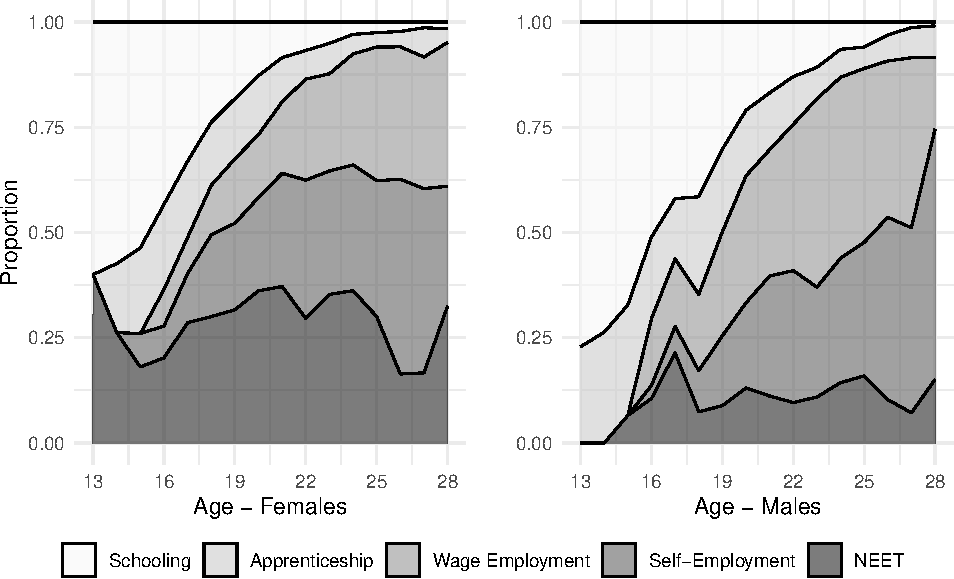
\includegraphics{figures/fig-ageplot-1} \caption{Occupation by age (recall data)}\label{fig:fig-ageplot}
\end{figure}

Table \ref{tab:tbl-pooledmatrix} depicts the rates of transition between activities pooled across the five detailed survey rounds, resulting in average transition rates over four transitions between the years of 2019 and 2021. As expected, the rate of graduation (transition out of school) is even higher than the last period of the event history. On average, 39.7 percent of youth changed activities between each survey round, a significantly higher rate than the 17 percent observed in the event history data, reflecting both the higher instability associated with the transition phase (compared to school-age years) and, potentially, more frequent variation in youth activity, particularly after graduation, than can be captured by annual data. The most stable activity is wage employment, with a 68\% retention rate across all survey rounds. The most common transitions are NEET to wage employment (128 transitions), NEET to self-employment (97), wage employed to NEET (93), self-employment to NEET (75) and school to NEET (66). School to wage employment (51) as well as self-employed to employed (48) and employed to self-employed (51) are also common. In terms of rates, the most likely transitions overall are from NEET to wage employment (22.18 percent of NEET youth transition to wage employment in the next period) and self-employment to NEET (20.78 percent). The most common transition for youth in school is NEET in the following period (16.22 percent); for the wage employed it is NEET (16.49 percent) and for apprentices it is NEET (19.44 percent). Other frequent transitions are NEET to self-employment (16.81 percent), self-employment to wage employment (13.3 percent), and employed to NEET (16.49 percent).

\newpage
\singlespacing

\providecommand{\docline}[3]{\noalign{\global\setlength{\arrayrulewidth}{#1}}\arrayrulecolor[HTML]{#2}\cline{#3}}

\setlength{\tabcolsep}{0pt}

\renewcommand*{\arraystretch}{1.15}

\begin{longtable}[c]{|p{1.20in}|p{0.80in}|p{0.80in}|p{0.80in}|p{0.80in}|p{0.80in}}

\caption{\textcolor[HTML]{000000}{\fontsize{11}{13}\selectfont{\global\setmainfont{Palatino}{Activity\ transition\ matrix:\ Combined\ data,\ 2013-2021}}}}\label{tab:tbl-matrix}\\

\hhline{~~~~~~}

\multicolumn{3}{!{\color[HTML]{000000}\vrule width 0pt}>{\raggedright}p{\dimexpr 2.8in+4\tabcolsep+2\arrayrulewidth}}{\textcolor[HTML]{000000}{\fontsize{9}{9}\selectfont{\global\setmainfont{Palatino}{}}}} & \multicolumn{3}{!{\color[HTML]{000000}\vrule width 0pt}>{\raggedright}p{\dimexpr 2.4in+4\tabcolsep+2\arrayrulewidth}!{\color[HTML]{000000}\vrule width 0pt}}{\textcolor[HTML]{000000}{\fontsize{9}{9}\selectfont{\global\setmainfont{Palatino}{To}}}} \\

\hhline{>{\arrayrulecolor[HTML]{666666}\global\arrayrulewidth=2pt}->{\arrayrulecolor[HTML]{666666}\global\arrayrulewidth=2pt}->{\arrayrulecolor[HTML]{666666}\global\arrayrulewidth=2pt}->{\arrayrulecolor[HTML]{666666}\global\arrayrulewidth=2pt}->{\arrayrulecolor[HTML]{666666}\global\arrayrulewidth=2pt}->{\arrayrulecolor[HTML]{666666}\global\arrayrulewidth=2pt}-}



\multicolumn{1}{!{\color[HTML]{000000}\vrule width 0pt}>{\raggedright}p{\dimexpr 1.2in+0\tabcolsep+0\arrayrulewidth}}{\textcolor[HTML]{000000}{\fontsize{9}{9}\selectfont{\global\setmainfont{Palatino}{From}}}} & \multicolumn{1}{!{\color[HTML]{000000}\vrule width 0pt}>{\raggedright}p{\dimexpr 0.8in+0\tabcolsep+0\arrayrulewidth}}{\textcolor[HTML]{000000}{\fontsize{9}{9}\selectfont{\global\setmainfont{Palatino}{In\ School}}}} & \multicolumn{1}{!{\color[HTML]{000000}\vrule width 0pt}>{\raggedright}p{\dimexpr 0.8in+0\tabcolsep+0\arrayrulewidth}}{\textcolor[HTML]{000000}{\fontsize{9}{9}\selectfont{\global\setmainfont{Palatino}{NEET}}}} & \multicolumn{1}{!{\color[HTML]{000000}\vrule width 0pt}>{\raggedright}p{\dimexpr 0.8in+0\tabcolsep+0\arrayrulewidth}}{\textcolor[HTML]{000000}{\fontsize{9}{9}\selectfont{\global\setmainfont{Palatino}{Self-Employed}}}} & \multicolumn{1}{!{\color[HTML]{000000}\vrule width 0pt}>{\raggedright}p{\dimexpr 0.8in+0\tabcolsep+0\arrayrulewidth}}{\textcolor[HTML]{000000}{\fontsize{9}{9}\selectfont{\global\setmainfont{Palatino}{Employed}}}} & \multicolumn{1}{!{\color[HTML]{000000}\vrule width 0pt}>{\raggedright}p{\dimexpr 0.8in+0\tabcolsep+0\arrayrulewidth}!{\color[HTML]{000000}\vrule width 0pt}}{\textcolor[HTML]{000000}{\fontsize{9}{9}\selectfont{\global\setmainfont{Palatino}{Apprentice}}}} \\

\hhline{>{\arrayrulecolor[HTML]{666666}\global\arrayrulewidth=2pt}->{\arrayrulecolor[HTML]{666666}\global\arrayrulewidth=2pt}->{\arrayrulecolor[HTML]{666666}\global\arrayrulewidth=2pt}->{\arrayrulecolor[HTML]{666666}\global\arrayrulewidth=2pt}->{\arrayrulecolor[HTML]{666666}\global\arrayrulewidth=2pt}->{\arrayrulecolor[HTML]{666666}\global\arrayrulewidth=2pt}-}\endhead



\multicolumn{6}{!{\color[HTML]{FFFFFF}\vrule width 0pt}>{\raggedright}p{\dimexpr 5.2in+10\tabcolsep+5\arrayrulewidth}!{\color[HTML]{FFFFFF}\vrule width 0pt}}{\textcolor[HTML]{000000}{\fontsize{9}{9}\selectfont{\global\setmainfont{Palatino}{Row\ \%.\ First\ row\ for\ each\ activity\ refers\ to\ unconditional\ transition\ rate;\ remaining\ rates\ are\ conditional.}}}} \\

\endfoot



\multicolumn{1}{!{\color[HTML]{000000}\vrule width 0pt}>{\raggedright}p{\dimexpr 1.2in+0\tabcolsep+0\arrayrulewidth}}{\textcolor[HTML]{000000}{\fontsize{9}{9}\selectfont{\global\setmainfont{Palatino}{\textbf{In\ School}}}}} & \multicolumn{1}{!{\color[HTML]{000000}\vrule width 0pt}>{\centering}p{\dimexpr 0.8in+0\tabcolsep+0\arrayrulewidth}}{\textcolor[HTML]{000000}{\fontsize{9}{9}\selectfont{\global\setmainfont{Palatino}{\textbf{85.68\%}}}}} & \multicolumn{1}{!{\color[HTML]{000000}\vrule width 0pt}>{\centering}p{\dimexpr 0.8in+0\tabcolsep+0\arrayrulewidth}}{\textcolor[HTML]{000000}{\fontsize{9}{9}\selectfont{\global\setmainfont{Palatino}{\textbf{3.85\%}}}}} & \multicolumn{1}{!{\color[HTML]{000000}\vrule width 0pt}>{\centering}p{\dimexpr 0.8in+0\tabcolsep+0\arrayrulewidth}}{\textcolor[HTML]{000000}{\fontsize{9}{9}\selectfont{\global\setmainfont{Palatino}{\textbf{2.61\%}}}}} & \multicolumn{1}{!{\color[HTML]{000000}\vrule width 0pt}>{\centering}p{\dimexpr 0.8in+0\tabcolsep+0\arrayrulewidth}}{\textcolor[HTML]{000000}{\fontsize{9}{9}\selectfont{\global\setmainfont{Palatino}{\textbf{4.92\%}}}}} & \multicolumn{1}{!{\color[HTML]{000000}\vrule width 0pt}>{\centering}p{\dimexpr 0.8in+0\tabcolsep+0\arrayrulewidth}!{\color[HTML]{000000}\vrule width 0pt}}{\textcolor[HTML]{000000}{\fontsize{9}{9}\selectfont{\global\setmainfont{Palatino}{\textbf{2.95\%}}}}} \\





\multicolumn{1}{!{\color[HTML]{000000}\vrule width 0pt}>{\raggedright}p{\dimexpr 1.2in+0\tabcolsep+0\arrayrulewidth}}{\textcolor[HTML]{000000}{\fontsize{9}{9}\selectfont{\global\setmainfont{Palatino}{Conditional}}}} & \multicolumn{1}{!{\color[HTML]{000000}\vrule width 0pt}>{\centering}p{\dimexpr 0.8in+0\tabcolsep+0\arrayrulewidth}}{\textcolor[HTML]{000000}{\fontsize{9}{9}\selectfont{\global\setmainfont{Palatino}{-}}}} & \multicolumn{1}{!{\color[HTML]{000000}\vrule width 0pt}>{\centering}p{\dimexpr 0.8in+0\tabcolsep+0\arrayrulewidth}}{\textcolor[HTML]{000000}{\fontsize{9}{9}\selectfont{\global\setmainfont{Palatino}{4.49\%}}}} & \multicolumn{1}{!{\color[HTML]{000000}\vrule width 0pt}>{\centering}p{\dimexpr 0.8in+0\tabcolsep+0\arrayrulewidth}}{\textcolor[HTML]{000000}{\fontsize{9}{9}\selectfont{\global\setmainfont{Palatino}{3.04\%}}}} & \multicolumn{1}{!{\color[HTML]{000000}\vrule width 0pt}>{\centering}p{\dimexpr 0.8in+0\tabcolsep+0\arrayrulewidth}}{\textcolor[HTML]{000000}{\fontsize{9}{9}\selectfont{\global\setmainfont{Palatino}{5.74\%}}}} & \multicolumn{1}{!{\color[HTML]{000000}\vrule width 0pt}>{\centering}p{\dimexpr 0.8in+0\tabcolsep+0\arrayrulewidth}!{\color[HTML]{000000}\vrule width 0pt}}{\textcolor[HTML]{000000}{\fontsize{9}{9}\selectfont{\global\setmainfont{Palatino}{3.44\%}}}} \\





\multicolumn{1}{!{\color[HTML]{000000}\vrule width 0pt}>{\raggedright}p{\dimexpr 1.2in+0\tabcolsep+0\arrayrulewidth}}{\textcolor[HTML]{000000}{\fontsize{9}{9}\selectfont{\global\setmainfont{Palatino}{Female}}}} & \multicolumn{1}{!{\color[HTML]{000000}\vrule width 0pt}>{\centering}p{\dimexpr 0.8in+0\tabcolsep+0\arrayrulewidth}}{\textcolor[HTML]{000000}{\fontsize{9}{9}\selectfont{\global\setmainfont{Palatino}{-}}}} & \multicolumn{1}{!{\color[HTML]{000000}\vrule width 0pt}>{\centering}p{\dimexpr 0.8in+0\tabcolsep+0\arrayrulewidth}}{\textcolor[HTML]{000000}{\fontsize{9}{9}\selectfont{\global\setmainfont{Palatino}{5.02\%}}}} & \multicolumn{1}{!{\color[HTML]{000000}\vrule width 0pt}>{\centering}p{\dimexpr 0.8in+0\tabcolsep+0\arrayrulewidth}}{\textcolor[HTML]{000000}{\fontsize{9}{9}\selectfont{\global\setmainfont{Palatino}{2.74\%}}}} & \multicolumn{1}{!{\color[HTML]{000000}\vrule width 0pt}>{\centering}p{\dimexpr 0.8in+0\tabcolsep+0\arrayrulewidth}}{\textcolor[HTML]{000000}{\fontsize{9}{9}\selectfont{\global\setmainfont{Palatino}{6.04\%}}}} & \multicolumn{1}{!{\color[HTML]{000000}\vrule width 0pt}>{\centering}p{\dimexpr 0.8in+0\tabcolsep+0\arrayrulewidth}!{\color[HTML]{000000}\vrule width 0pt}}{\textcolor[HTML]{000000}{\fontsize{9}{9}\selectfont{\global\setmainfont{Palatino}{4.45\%}}}} \\





\multicolumn{1}{!{\color[HTML]{000000}\vrule width 0pt}>{\raggedright}p{\dimexpr 1.2in+0\tabcolsep+0\arrayrulewidth}}{\textcolor[HTML]{000000}{\fontsize{9}{9}\selectfont{\global\setmainfont{Palatino}{Male}}}} & \multicolumn{1}{!{\color[HTML]{000000}\vrule width 0pt}>{\centering}p{\dimexpr 0.8in+0\tabcolsep+0\arrayrulewidth}}{\textcolor[HTML]{000000}{\fontsize{9}{9}\selectfont{\global\setmainfont{Palatino}{-}}}} & \multicolumn{1}{!{\color[HTML]{000000}\vrule width 0pt}>{\centering}p{\dimexpr 0.8in+0\tabcolsep+0\arrayrulewidth}}{\textcolor[HTML]{000000}{\fontsize{9}{9}\selectfont{\global\setmainfont{Palatino}{4.08\%}}}} & \multicolumn{1}{!{\color[HTML]{000000}\vrule width 0pt}>{\centering}p{\dimexpr 0.8in+0\tabcolsep+0\arrayrulewidth}}{\textcolor[HTML]{000000}{\fontsize{9}{9}\selectfont{\global\setmainfont{Palatino}{3.28\%}}}} & \multicolumn{1}{!{\color[HTML]{000000}\vrule width 0pt}>{\centering}p{\dimexpr 0.8in+0\tabcolsep+0\arrayrulewidth}}{\textcolor[HTML]{000000}{\fontsize{9}{9}\selectfont{\global\setmainfont{Palatino}{5.50\%}}}} & \multicolumn{1}{!{\color[HTML]{000000}\vrule width 0pt}>{\centering}p{\dimexpr 0.8in+0\tabcolsep+0\arrayrulewidth}!{\color[HTML]{000000}\vrule width 0pt}}{\textcolor[HTML]{000000}{\fontsize{9}{9}\selectfont{\global\setmainfont{Palatino}{2.66\%}}}} \\





\multicolumn{1}{!{\color[HTML]{000000}\vrule width 0pt}>{\raggedright}p{\dimexpr 1.2in+0\tabcolsep+0\arrayrulewidth}}{\textcolor[HTML]{000000}{\fontsize{9}{9}\selectfont{\global\setmainfont{Palatino}{14-18}}}} & \multicolumn{1}{!{\color[HTML]{000000}\vrule width 0pt}>{\centering}p{\dimexpr 0.8in+0\tabcolsep+0\arrayrulewidth}}{\textcolor[HTML]{000000}{\fontsize{9}{9}\selectfont{\global\setmainfont{Palatino}{-}}}} & \multicolumn{1}{!{\color[HTML]{000000}\vrule width 0pt}>{\centering}p{\dimexpr 0.8in+0\tabcolsep+0\arrayrulewidth}}{\textcolor[HTML]{000000}{\fontsize{9}{9}\selectfont{\global\setmainfont{Palatino}{1.32\%}}}} & \multicolumn{1}{!{\color[HTML]{000000}\vrule width 0pt}>{\centering}p{\dimexpr 0.8in+0\tabcolsep+0\arrayrulewidth}}{\textcolor[HTML]{000000}{\fontsize{9}{9}\selectfont{\global\setmainfont{Palatino}{1.08\%}}}} & \multicolumn{1}{!{\color[HTML]{000000}\vrule width 0pt}>{\centering}p{\dimexpr 0.8in+0\tabcolsep+0\arrayrulewidth}}{\textcolor[HTML]{000000}{\fontsize{9}{9}\selectfont{\global\setmainfont{Palatino}{0.96\%}}}} & \multicolumn{1}{!{\color[HTML]{000000}\vrule width 0pt}>{\centering}p{\dimexpr 0.8in+0\tabcolsep+0\arrayrulewidth}!{\color[HTML]{000000}\vrule width 0pt}}{\textcolor[HTML]{000000}{\fontsize{9}{9}\selectfont{\global\setmainfont{Palatino}{2.15\%}}}} \\





\multicolumn{1}{!{\color[HTML]{000000}\vrule width 0pt}>{\raggedright}p{\dimexpr 1.2in+0\tabcolsep+0\arrayrulewidth}}{\textcolor[HTML]{000000}{\fontsize{9}{9}\selectfont{\global\setmainfont{Palatino}{19-24}}}} & \multicolumn{1}{!{\color[HTML]{000000}\vrule width 0pt}>{\centering}p{\dimexpr 0.8in+0\tabcolsep+0\arrayrulewidth}}{\textcolor[HTML]{000000}{\fontsize{9}{9}\selectfont{\global\setmainfont{Palatino}{-}}}} & \multicolumn{1}{!{\color[HTML]{000000}\vrule width 0pt}>{\centering}p{\dimexpr 0.8in+0\tabcolsep+0\arrayrulewidth}}{\textcolor[HTML]{000000}{\fontsize{9}{9}\selectfont{\global\setmainfont{Palatino}{6.23\%}}}} & \multicolumn{1}{!{\color[HTML]{000000}\vrule width 0pt}>{\centering}p{\dimexpr 0.8in+0\tabcolsep+0\arrayrulewidth}}{\textcolor[HTML]{000000}{\fontsize{9}{9}\selectfont{\global\setmainfont{Palatino}{3.94\%}}}} & \multicolumn{1}{!{\color[HTML]{000000}\vrule width 0pt}>{\centering}p{\dimexpr 0.8in+0\tabcolsep+0\arrayrulewidth}}{\textcolor[HTML]{000000}{\fontsize{9}{9}\selectfont{\global\setmainfont{Palatino}{8.42\%}}}} & \multicolumn{1}{!{\color[HTML]{000000}\vrule width 0pt}>{\centering}p{\dimexpr 0.8in+0\tabcolsep+0\arrayrulewidth}!{\color[HTML]{000000}\vrule width 0pt}}{\textcolor[HTML]{000000}{\fontsize{9}{9}\selectfont{\global\setmainfont{Palatino}{4.40\%}}}} \\





\multicolumn{1}{!{\color[HTML]{000000}\vrule width 0pt}>{\raggedright}p{\dimexpr 1.2in+0\tabcolsep+0\arrayrulewidth}}{\textcolor[HTML]{000000}{\fontsize{9}{9}\selectfont{\global\setmainfont{Palatino}{25-30}}}} & \multicolumn{1}{!{\color[HTML]{000000}\vrule width 0pt}>{\centering}p{\dimexpr 0.8in+0\tabcolsep+0\arrayrulewidth}}{\textcolor[HTML]{000000}{\fontsize{9}{9}\selectfont{\global\setmainfont{Palatino}{-}}}} & \multicolumn{1}{!{\color[HTML]{000000}\vrule width 0pt}>{\centering}p{\dimexpr 0.8in+0\tabcolsep+0\arrayrulewidth}}{\textcolor[HTML]{000000}{\fontsize{9}{9}\selectfont{\global\setmainfont{Palatino}{14.47\%}}}} & \multicolumn{1}{!{\color[HTML]{000000}\vrule width 0pt}>{\centering}p{\dimexpr 0.8in+0\tabcolsep+0\arrayrulewidth}}{\textcolor[HTML]{000000}{\fontsize{9}{9}\selectfont{\global\setmainfont{Palatino}{11.84\%}}}} & \multicolumn{1}{!{\color[HTML]{000000}\vrule width 0pt}>{\centering}p{\dimexpr 0.8in+0\tabcolsep+0\arrayrulewidth}}{\textcolor[HTML]{000000}{\fontsize{9}{9}\selectfont{\global\setmainfont{Palatino}{19.74\%}}}} & \multicolumn{1}{!{\color[HTML]{000000}\vrule width 0pt}>{\centering}p{\dimexpr 0.8in+0\tabcolsep+0\arrayrulewidth}!{\color[HTML]{000000}\vrule width 0pt}}{\textcolor[HTML]{000000}{\fontsize{9}{9}\selectfont{\global\setmainfont{Palatino}{3.95\%}}}} \\





\multicolumn{1}{!{\color[HTML]{000000}\vrule width 0pt}>{\raggedright}p{\dimexpr 1.2in+0\tabcolsep+0\arrayrulewidth}}{\textcolor[HTML]{000000}{\fontsize{9}{9}\selectfont{\global\setmainfont{Palatino}{\textbf{NEET}}}}} & \multicolumn{1}{!{\color[HTML]{000000}\vrule width 0pt}>{\centering}p{\dimexpr 0.8in+0\tabcolsep+0\arrayrulewidth}}{\textcolor[HTML]{000000}{\fontsize{9}{9}\selectfont{\global\setmainfont{Palatino}{\textbf{1.82\%}}}}} & \multicolumn{1}{!{\color[HTML]{000000}\vrule width 0pt}>{\centering}p{\dimexpr 0.8in+0\tabcolsep+0\arrayrulewidth}}{\textcolor[HTML]{000000}{\fontsize{9}{9}\selectfont{\global\setmainfont{Palatino}{\textbf{64.94\%}}}}} & \multicolumn{1}{!{\color[HTML]{000000}\vrule width 0pt}>{\centering}p{\dimexpr 0.8in+0\tabcolsep+0\arrayrulewidth}}{\textcolor[HTML]{000000}{\fontsize{9}{9}\selectfont{\global\setmainfont{Palatino}{\textbf{11.17\%}}}}} & \multicolumn{1}{!{\color[HTML]{000000}\vrule width 0pt}>{\centering}p{\dimexpr 0.8in+0\tabcolsep+0\arrayrulewidth}}{\textcolor[HTML]{000000}{\fontsize{9}{9}\selectfont{\global\setmainfont{Palatino}{\textbf{14.29\%}}}}} & \multicolumn{1}{!{\color[HTML]{000000}\vrule width 0pt}>{\centering}p{\dimexpr 0.8in+0\tabcolsep+0\arrayrulewidth}!{\color[HTML]{000000}\vrule width 0pt}}{\textcolor[HTML]{000000}{\fontsize{9}{9}\selectfont{\global\setmainfont{Palatino}{\textbf{7.79\%}}}}} \\





\multicolumn{1}{!{\color[HTML]{000000}\vrule width 0pt}>{\raggedright}p{\dimexpr 1.2in+0\tabcolsep+0\arrayrulewidth}}{\textcolor[HTML]{000000}{\fontsize{9}{9}\selectfont{\global\setmainfont{Palatino}{Conditional}}}} & \multicolumn{1}{!{\color[HTML]{000000}\vrule width 0pt}>{\centering}p{\dimexpr 0.8in+0\tabcolsep+0\arrayrulewidth}}{\textcolor[HTML]{000000}{\fontsize{9}{9}\selectfont{\global\setmainfont{Palatino}{2.80\%}}}} & \multicolumn{1}{!{\color[HTML]{000000}\vrule width 0pt}>{\centering}p{\dimexpr 0.8in+0\tabcolsep+0\arrayrulewidth}}{\textcolor[HTML]{000000}{\fontsize{9}{9}\selectfont{\global\setmainfont{Palatino}{-}}}} & \multicolumn{1}{!{\color[HTML]{000000}\vrule width 0pt}>{\centering}p{\dimexpr 0.8in+0\tabcolsep+0\arrayrulewidth}}{\textcolor[HTML]{000000}{\fontsize{9}{9}\selectfont{\global\setmainfont{Palatino}{17.20\%}}}} & \multicolumn{1}{!{\color[HTML]{000000}\vrule width 0pt}>{\centering}p{\dimexpr 0.8in+0\tabcolsep+0\arrayrulewidth}}{\textcolor[HTML]{000000}{\fontsize{9}{9}\selectfont{\global\setmainfont{Palatino}{22.00\%}}}} & \multicolumn{1}{!{\color[HTML]{000000}\vrule width 0pt}>{\centering}p{\dimexpr 0.8in+0\tabcolsep+0\arrayrulewidth}!{\color[HTML]{000000}\vrule width 0pt}}{\textcolor[HTML]{000000}{\fontsize{9}{9}\selectfont{\global\setmainfont{Palatino}{12.00\%}}}} \\





\multicolumn{1}{!{\color[HTML]{000000}\vrule width 0pt}>{\raggedright}p{\dimexpr 1.2in+0\tabcolsep+0\arrayrulewidth}}{\textcolor[HTML]{000000}{\fontsize{9}{9}\selectfont{\global\setmainfont{Palatino}{Female}}}} & \multicolumn{1}{!{\color[HTML]{000000}\vrule width 0pt}>{\centering}p{\dimexpr 0.8in+0\tabcolsep+0\arrayrulewidth}}{\textcolor[HTML]{000000}{\fontsize{9}{9}\selectfont{\global\setmainfont{Palatino}{2.33\%}}}} & \multicolumn{1}{!{\color[HTML]{000000}\vrule width 0pt}>{\centering}p{\dimexpr 0.8in+0\tabcolsep+0\arrayrulewidth}}{\textcolor[HTML]{000000}{\fontsize{9}{9}\selectfont{\global\setmainfont{Palatino}{-}}}} & \multicolumn{1}{!{\color[HTML]{000000}\vrule width 0pt}>{\centering}p{\dimexpr 0.8in+0\tabcolsep+0\arrayrulewidth}}{\textcolor[HTML]{000000}{\fontsize{9}{9}\selectfont{\global\setmainfont{Palatino}{13.95\%}}}} & \multicolumn{1}{!{\color[HTML]{000000}\vrule width 0pt}>{\centering}p{\dimexpr 0.8in+0\tabcolsep+0\arrayrulewidth}}{\textcolor[HTML]{000000}{\fontsize{9}{9}\selectfont{\global\setmainfont{Palatino}{15.35\%}}}} & \multicolumn{1}{!{\color[HTML]{000000}\vrule width 0pt}>{\centering}p{\dimexpr 0.8in+0\tabcolsep+0\arrayrulewidth}!{\color[HTML]{000000}\vrule width 0pt}}{\textcolor[HTML]{000000}{\fontsize{9}{9}\selectfont{\global\setmainfont{Palatino}{7.91\%}}}} \\





\multicolumn{1}{!{\color[HTML]{000000}\vrule width 0pt}>{\raggedright}p{\dimexpr 1.2in+0\tabcolsep+0\arrayrulewidth}}{\textcolor[HTML]{000000}{\fontsize{9}{9}\selectfont{\global\setmainfont{Palatino}{Male}}}} & \multicolumn{1}{!{\color[HTML]{000000}\vrule width 0pt}>{\centering}p{\dimexpr 0.8in+0\tabcolsep+0\arrayrulewidth}}{\textcolor[HTML]{000000}{\fontsize{9}{9}\selectfont{\global\setmainfont{Palatino}{5.71\%}}}} & \multicolumn{1}{!{\color[HTML]{000000}\vrule width 0pt}>{\centering}p{\dimexpr 0.8in+0\tabcolsep+0\arrayrulewidth}}{\textcolor[HTML]{000000}{\fontsize{9}{9}\selectfont{\global\setmainfont{Palatino}{-}}}} & \multicolumn{1}{!{\color[HTML]{000000}\vrule width 0pt}>{\centering}p{\dimexpr 0.8in+0\tabcolsep+0\arrayrulewidth}}{\textcolor[HTML]{000000}{\fontsize{9}{9}\selectfont{\global\setmainfont{Palatino}{37.14\%}}}} & \multicolumn{1}{!{\color[HTML]{000000}\vrule width 0pt}>{\centering}p{\dimexpr 0.8in+0\tabcolsep+0\arrayrulewidth}}{\textcolor[HTML]{000000}{\fontsize{9}{9}\selectfont{\global\setmainfont{Palatino}{62.86\%}}}} & \multicolumn{1}{!{\color[HTML]{000000}\vrule width 0pt}>{\centering}p{\dimexpr 0.8in+0\tabcolsep+0\arrayrulewidth}!{\color[HTML]{000000}\vrule width 0pt}}{\textcolor[HTML]{000000}{\fontsize{9}{9}\selectfont{\global\setmainfont{Palatino}{37.14\%}}}} \\





\multicolumn{1}{!{\color[HTML]{000000}\vrule width 0pt}>{\raggedright}p{\dimexpr 1.2in+0\tabcolsep+0\arrayrulewidth}}{\textcolor[HTML]{000000}{\fontsize{9}{9}\selectfont{\global\setmainfont{Palatino}{14-18}}}} & \multicolumn{1}{!{\color[HTML]{000000}\vrule width 0pt}>{\centering}p{\dimexpr 0.8in+0\tabcolsep+0\arrayrulewidth}}{\textcolor[HTML]{000000}{\fontsize{9}{9}\selectfont{\global\setmainfont{Palatino}{4.76\%}}}} & \multicolumn{1}{!{\color[HTML]{000000}\vrule width 0pt}>{\centering}p{\dimexpr 0.8in+0\tabcolsep+0\arrayrulewidth}}{\textcolor[HTML]{000000}{\fontsize{9}{9}\selectfont{\global\setmainfont{Palatino}{-}}}} & \multicolumn{1}{!{\color[HTML]{000000}\vrule width 0pt}>{\centering}p{\dimexpr 0.8in+0\tabcolsep+0\arrayrulewidth}}{\textcolor[HTML]{000000}{\fontsize{9}{9}\selectfont{\global\setmainfont{Palatino}{7.14\%}}}} & \multicolumn{1}{!{\color[HTML]{000000}\vrule width 0pt}>{\centering}p{\dimexpr 0.8in+0\tabcolsep+0\arrayrulewidth}}{\textcolor[HTML]{000000}{\fontsize{9}{9}\selectfont{\global\setmainfont{Palatino}{11.90\%}}}} & \multicolumn{1}{!{\color[HTML]{000000}\vrule width 0pt}>{\centering}p{\dimexpr 0.8in+0\tabcolsep+0\arrayrulewidth}!{\color[HTML]{000000}\vrule width 0pt}}{\textcolor[HTML]{000000}{\fontsize{9}{9}\selectfont{\global\setmainfont{Palatino}{21.43\%}}}} \\





\multicolumn{1}{!{\color[HTML]{000000}\vrule width 0pt}>{\raggedright}p{\dimexpr 1.2in+0\tabcolsep+0\arrayrulewidth}}{\textcolor[HTML]{000000}{\fontsize{9}{9}\selectfont{\global\setmainfont{Palatino}{19-24}}}} & \multicolumn{1}{!{\color[HTML]{000000}\vrule width 0pt}>{\centering}p{\dimexpr 0.8in+0\tabcolsep+0\arrayrulewidth}}{\textcolor[HTML]{000000}{\fontsize{9}{9}\selectfont{\global\setmainfont{Palatino}{2.31\%}}}} & \multicolumn{1}{!{\color[HTML]{000000}\vrule width 0pt}>{\centering}p{\dimexpr 0.8in+0\tabcolsep+0\arrayrulewidth}}{\textcolor[HTML]{000000}{\fontsize{9}{9}\selectfont{\global\setmainfont{Palatino}{-}}}} & \multicolumn{1}{!{\color[HTML]{000000}\vrule width 0pt}>{\centering}p{\dimexpr 0.8in+0\tabcolsep+0\arrayrulewidth}}{\textcolor[HTML]{000000}{\fontsize{9}{9}\selectfont{\global\setmainfont{Palatino}{16.18\%}}}} & \multicolumn{1}{!{\color[HTML]{000000}\vrule width 0pt}>{\centering}p{\dimexpr 0.8in+0\tabcolsep+0\arrayrulewidth}}{\textcolor[HTML]{000000}{\fontsize{9}{9}\selectfont{\global\setmainfont{Palatino}{18.50\%}}}} & \multicolumn{1}{!{\color[HTML]{000000}\vrule width 0pt}>{\centering}p{\dimexpr 0.8in+0\tabcolsep+0\arrayrulewidth}!{\color[HTML]{000000}\vrule width 0pt}}{\textcolor[HTML]{000000}{\fontsize{9}{9}\selectfont{\global\setmainfont{Palatino}{9.83\%}}}} \\





\multicolumn{1}{!{\color[HTML]{000000}\vrule width 0pt}>{\raggedright}p{\dimexpr 1.2in+0\tabcolsep+0\arrayrulewidth}}{\textcolor[HTML]{000000}{\fontsize{9}{9}\selectfont{\global\setmainfont{Palatino}{25-30}}}} & \multicolumn{1}{!{\color[HTML]{000000}\vrule width 0pt}>{\centering}p{\dimexpr 0.8in+0\tabcolsep+0\arrayrulewidth}}{\textcolor[HTML]{000000}{\fontsize{9}{9}\selectfont{\global\setmainfont{Palatino}{2.86\%}}}} & \multicolumn{1}{!{\color[HTML]{000000}\vrule width 0pt}>{\centering}p{\dimexpr 0.8in+0\tabcolsep+0\arrayrulewidth}}{\textcolor[HTML]{000000}{\fontsize{9}{9}\selectfont{\global\setmainfont{Palatino}{-}}}} & \multicolumn{1}{!{\color[HTML]{000000}\vrule width 0pt}>{\centering}p{\dimexpr 0.8in+0\tabcolsep+0\arrayrulewidth}}{\textcolor[HTML]{000000}{\fontsize{9}{9}\selectfont{\global\setmainfont{Palatino}{34.29\%}}}} & \multicolumn{1}{!{\color[HTML]{000000}\vrule width 0pt}>{\centering}p{\dimexpr 0.8in+0\tabcolsep+0\arrayrulewidth}}{\textcolor[HTML]{000000}{\fontsize{9}{9}\selectfont{\global\setmainfont{Palatino}{51.43\%}}}} & \multicolumn{1}{!{\color[HTML]{000000}\vrule width 0pt}>{\centering}p{\dimexpr 0.8in+0\tabcolsep+0\arrayrulewidth}!{\color[HTML]{000000}\vrule width 0pt}}{\textcolor[HTML]{000000}{\fontsize{9}{9}\selectfont{\global\setmainfont{Palatino}{11.43\%}}}} \\





\multicolumn{1}{!{\color[HTML]{000000}\vrule width 0pt}>{\raggedright}p{\dimexpr 1.2in+0\tabcolsep+0\arrayrulewidth}}{\textcolor[HTML]{000000}{\fontsize{9}{9}\selectfont{\global\setmainfont{Palatino}{\textbf{Self-Employed}}}}} & \multicolumn{1}{!{\color[HTML]{000000}\vrule width 0pt}>{\centering}p{\dimexpr 0.8in+0\tabcolsep+0\arrayrulewidth}}{\textcolor[HTML]{000000}{\fontsize{9}{9}\selectfont{\global\setmainfont{Palatino}{\textbf{1.87\%}}}}} & \multicolumn{1}{!{\color[HTML]{000000}\vrule width 0pt}>{\centering}p{\dimexpr 0.8in+0\tabcolsep+0\arrayrulewidth}}{\textcolor[HTML]{000000}{\fontsize{9}{9}\selectfont{\global\setmainfont{Palatino}{\textbf{4.68\%}}}}} & \multicolumn{1}{!{\color[HTML]{000000}\vrule width 0pt}>{\centering}p{\dimexpr 0.8in+0\tabcolsep+0\arrayrulewidth}}{\textcolor[HTML]{000000}{\fontsize{9}{9}\selectfont{\global\setmainfont{Palatino}{\textbf{87.82\%}}}}} & \multicolumn{1}{!{\color[HTML]{000000}\vrule width 0pt}>{\centering}p{\dimexpr 0.8in+0\tabcolsep+0\arrayrulewidth}}{\textcolor[HTML]{000000}{\fontsize{9}{9}\selectfont{\global\setmainfont{Palatino}{\textbf{3.75\%}}}}} & \multicolumn{1}{!{\color[HTML]{000000}\vrule width 0pt}>{\centering}p{\dimexpr 0.8in+0\tabcolsep+0\arrayrulewidth}!{\color[HTML]{000000}\vrule width 0pt}}{\textcolor[HTML]{000000}{\fontsize{9}{9}\selectfont{\global\setmainfont{Palatino}{\textbf{1.87\%}}}}} \\





\multicolumn{1}{!{\color[HTML]{000000}\vrule width 0pt}>{\raggedright}p{\dimexpr 1.2in+0\tabcolsep+0\arrayrulewidth}}{\textcolor[HTML]{000000}{\fontsize{9}{9}\selectfont{\global\setmainfont{Palatino}{Conditional}}}} & \multicolumn{1}{!{\color[HTML]{000000}\vrule width 0pt}>{\centering}p{\dimexpr 0.8in+0\tabcolsep+0\arrayrulewidth}}{\textcolor[HTML]{000000}{\fontsize{9}{9}\selectfont{\global\setmainfont{Palatino}{2.13\%}}}} & \multicolumn{1}{!{\color[HTML]{000000}\vrule width 0pt}>{\centering}p{\dimexpr 0.8in+0\tabcolsep+0\arrayrulewidth}}{\textcolor[HTML]{000000}{\fontsize{9}{9}\selectfont{\global\setmainfont{Palatino}{5.33\%}}}} & \multicolumn{1}{!{\color[HTML]{000000}\vrule width 0pt}>{\centering}p{\dimexpr 0.8in+0\tabcolsep+0\arrayrulewidth}}{\textcolor[HTML]{000000}{\fontsize{9}{9}\selectfont{\global\setmainfont{Palatino}{-}}}} & \multicolumn{1}{!{\color[HTML]{000000}\vrule width 0pt}>{\centering}p{\dimexpr 0.8in+0\tabcolsep+0\arrayrulewidth}}{\textcolor[HTML]{000000}{\fontsize{9}{9}\selectfont{\global\setmainfont{Palatino}{4.27\%}}}} & \multicolumn{1}{!{\color[HTML]{000000}\vrule width 0pt}>{\centering}p{\dimexpr 0.8in+0\tabcolsep+0\arrayrulewidth}!{\color[HTML]{000000}\vrule width 0pt}}{\textcolor[HTML]{000000}{\fontsize{9}{9}\selectfont{\global\setmainfont{Palatino}{2.13\%}}}} \\





\multicolumn{1}{!{\color[HTML]{000000}\vrule width 0pt}>{\raggedright}p{\dimexpr 1.2in+0\tabcolsep+0\arrayrulewidth}}{\textcolor[HTML]{000000}{\fontsize{9}{9}\selectfont{\global\setmainfont{Palatino}{Female}}}} & \multicolumn{1}{!{\color[HTML]{000000}\vrule width 0pt}>{\centering}p{\dimexpr 0.8in+0\tabcolsep+0\arrayrulewidth}}{\textcolor[HTML]{000000}{\fontsize{9}{9}\selectfont{\global\setmainfont{Palatino}{0.96\%}}}} & \multicolumn{1}{!{\color[HTML]{000000}\vrule width 0pt}>{\centering}p{\dimexpr 0.8in+0\tabcolsep+0\arrayrulewidth}}{\textcolor[HTML]{000000}{\fontsize{9}{9}\selectfont{\global\setmainfont{Palatino}{6.22\%}}}} & \multicolumn{1}{!{\color[HTML]{000000}\vrule width 0pt}>{\centering}p{\dimexpr 0.8in+0\tabcolsep+0\arrayrulewidth}}{\textcolor[HTML]{000000}{\fontsize{9}{9}\selectfont{\global\setmainfont{Palatino}{-}}}} & \multicolumn{1}{!{\color[HTML]{000000}\vrule width 0pt}>{\centering}p{\dimexpr 0.8in+0\tabcolsep+0\arrayrulewidth}}{\textcolor[HTML]{000000}{\fontsize{9}{9}\selectfont{\global\setmainfont{Palatino}{4.31\%}}}} & \multicolumn{1}{!{\color[HTML]{000000}\vrule width 0pt}>{\centering}p{\dimexpr 0.8in+0\tabcolsep+0\arrayrulewidth}!{\color[HTML]{000000}\vrule width 0pt}}{\textcolor[HTML]{000000}{\fontsize{9}{9}\selectfont{\global\setmainfont{Palatino}{2.87\%}}}} \\





\multicolumn{1}{!{\color[HTML]{000000}\vrule width 0pt}>{\raggedright}p{\dimexpr 1.2in+0\tabcolsep+0\arrayrulewidth}}{\textcolor[HTML]{000000}{\fontsize{9}{9}\selectfont{\global\setmainfont{Palatino}{Male}}}} & \multicolumn{1}{!{\color[HTML]{000000}\vrule width 0pt}>{\centering}p{\dimexpr 0.8in+0\tabcolsep+0\arrayrulewidth}}{\textcolor[HTML]{000000}{\fontsize{9}{9}\selectfont{\global\setmainfont{Palatino}{3.61\%}}}} & \multicolumn{1}{!{\color[HTML]{000000}\vrule width 0pt}>{\centering}p{\dimexpr 0.8in+0\tabcolsep+0\arrayrulewidth}}{\textcolor[HTML]{000000}{\fontsize{9}{9}\selectfont{\global\setmainfont{Palatino}{4.22\%}}}} & \multicolumn{1}{!{\color[HTML]{000000}\vrule width 0pt}>{\centering}p{\dimexpr 0.8in+0\tabcolsep+0\arrayrulewidth}}{\textcolor[HTML]{000000}{\fontsize{9}{9}\selectfont{\global\setmainfont{Palatino}{-}}}} & \multicolumn{1}{!{\color[HTML]{000000}\vrule width 0pt}>{\centering}p{\dimexpr 0.8in+0\tabcolsep+0\arrayrulewidth}}{\textcolor[HTML]{000000}{\fontsize{9}{9}\selectfont{\global\setmainfont{Palatino}{4.22\%}}}} & \multicolumn{1}{!{\color[HTML]{000000}\vrule width 0pt}>{\centering}p{\dimexpr 0.8in+0\tabcolsep+0\arrayrulewidth}!{\color[HTML]{000000}\vrule width 0pt}}{\textcolor[HTML]{000000}{\fontsize{9}{9}\selectfont{\global\setmainfont{Palatino}{1.20\%}}}} \\





\multicolumn{1}{!{\color[HTML]{000000}\vrule width 0pt}>{\raggedright}p{\dimexpr 1.2in+0\tabcolsep+0\arrayrulewidth}}{\textcolor[HTML]{000000}{\fontsize{9}{9}\selectfont{\global\setmainfont{Palatino}{14-18}}}} & \multicolumn{1}{!{\color[HTML]{000000}\vrule width 0pt}>{\centering}p{\dimexpr 0.8in+0\tabcolsep+0\arrayrulewidth}}{\textcolor[HTML]{000000}{\fontsize{9}{9}\selectfont{\global\setmainfont{Palatino}{0.00\%}}}} & \multicolumn{1}{!{\color[HTML]{000000}\vrule width 0pt}>{\centering}p{\dimexpr 0.8in+0\tabcolsep+0\arrayrulewidth}}{\textcolor[HTML]{000000}{\fontsize{9}{9}\selectfont{\global\setmainfont{Palatino}{0.00\%}}}} & \multicolumn{1}{!{\color[HTML]{000000}\vrule width 0pt}>{\centering}p{\dimexpr 0.8in+0\tabcolsep+0\arrayrulewidth}}{\textcolor[HTML]{000000}{\fontsize{9}{9}\selectfont{\global\setmainfont{Palatino}{-}}}} & \multicolumn{1}{!{\color[HTML]{000000}\vrule width 0pt}>{\centering}p{\dimexpr 0.8in+0\tabcolsep+0\arrayrulewidth}}{\textcolor[HTML]{000000}{\fontsize{9}{9}\selectfont{\global\setmainfont{Palatino}{0.00\%}}}} & \multicolumn{1}{!{\color[HTML]{000000}\vrule width 0pt}>{\centering}p{\dimexpr 0.8in+0\tabcolsep+0\arrayrulewidth}!{\color[HTML]{000000}\vrule width 0pt}}{\textcolor[HTML]{000000}{\fontsize{9}{9}\selectfont{\global\setmainfont{Palatino}{14.29\%}}}} \\





\multicolumn{1}{!{\color[HTML]{000000}\vrule width 0pt}>{\raggedright}p{\dimexpr 1.2in+0\tabcolsep+0\arrayrulewidth}}{\textcolor[HTML]{000000}{\fontsize{9}{9}\selectfont{\global\setmainfont{Palatino}{19-24}}}} & \multicolumn{1}{!{\color[HTML]{000000}\vrule width 0pt}>{\centering}p{\dimexpr 0.8in+0\tabcolsep+0\arrayrulewidth}}{\textcolor[HTML]{000000}{\fontsize{9}{9}\selectfont{\global\setmainfont{Palatino}{2.90\%}}}} & \multicolumn{1}{!{\color[HTML]{000000}\vrule width 0pt}>{\centering}p{\dimexpr 0.8in+0\tabcolsep+0\arrayrulewidth}}{\textcolor[HTML]{000000}{\fontsize{9}{9}\selectfont{\global\setmainfont{Palatino}{6.22\%}}}} & \multicolumn{1}{!{\color[HTML]{000000}\vrule width 0pt}>{\centering}p{\dimexpr 0.8in+0\tabcolsep+0\arrayrulewidth}}{\textcolor[HTML]{000000}{\fontsize{9}{9}\selectfont{\global\setmainfont{Palatino}{-}}}} & \multicolumn{1}{!{\color[HTML]{000000}\vrule width 0pt}>{\centering}p{\dimexpr 0.8in+0\tabcolsep+0\arrayrulewidth}}{\textcolor[HTML]{000000}{\fontsize{9}{9}\selectfont{\global\setmainfont{Palatino}{5.39\%}}}} & \multicolumn{1}{!{\color[HTML]{000000}\vrule width 0pt}>{\centering}p{\dimexpr 0.8in+0\tabcolsep+0\arrayrulewidth}!{\color[HTML]{000000}\vrule width 0pt}}{\textcolor[HTML]{000000}{\fontsize{9}{9}\selectfont{\global\setmainfont{Palatino}{1.66\%}}}} \\





\multicolumn{1}{!{\color[HTML]{000000}\vrule width 0pt}>{\raggedright}p{\dimexpr 1.2in+0\tabcolsep+0\arrayrulewidth}}{\textcolor[HTML]{000000}{\fontsize{9}{9}\selectfont{\global\setmainfont{Palatino}{25-30}}}} & \multicolumn{1}{!{\color[HTML]{000000}\vrule width 0pt}>{\centering}p{\dimexpr 0.8in+0\tabcolsep+0\arrayrulewidth}}{\textcolor[HTML]{000000}{\fontsize{9}{9}\selectfont{\global\setmainfont{Palatino}{0.83\%}}}} & \multicolumn{1}{!{\color[HTML]{000000}\vrule width 0pt}>{\centering}p{\dimexpr 0.8in+0\tabcolsep+0\arrayrulewidth}}{\textcolor[HTML]{000000}{\fontsize{9}{9}\selectfont{\global\setmainfont{Palatino}{4.17\%}}}} & \multicolumn{1}{!{\color[HTML]{000000}\vrule width 0pt}>{\centering}p{\dimexpr 0.8in+0\tabcolsep+0\arrayrulewidth}}{\textcolor[HTML]{000000}{\fontsize{9}{9}\selectfont{\global\setmainfont{Palatino}{-}}}} & \multicolumn{1}{!{\color[HTML]{000000}\vrule width 0pt}>{\centering}p{\dimexpr 0.8in+0\tabcolsep+0\arrayrulewidth}}{\textcolor[HTML]{000000}{\fontsize{9}{9}\selectfont{\global\setmainfont{Palatino}{2.50\%}}}} & \multicolumn{1}{!{\color[HTML]{000000}\vrule width 0pt}>{\centering}p{\dimexpr 0.8in+0\tabcolsep+0\arrayrulewidth}!{\color[HTML]{000000}\vrule width 0pt}}{\textcolor[HTML]{000000}{\fontsize{9}{9}\selectfont{\global\setmainfont{Palatino}{1.67\%}}}} \\





\multicolumn{1}{!{\color[HTML]{000000}\vrule width 0pt}>{\raggedright}p{\dimexpr 1.2in+0\tabcolsep+0\arrayrulewidth}}{\textcolor[HTML]{000000}{\fontsize{9}{9}\selectfont{\global\setmainfont{Palatino}{\textbf{Employed}}}}} & \multicolumn{1}{!{\color[HTML]{000000}\vrule width 0pt}>{\centering}p{\dimexpr 0.8in+0\tabcolsep+0\arrayrulewidth}}{\textcolor[HTML]{000000}{\fontsize{9}{9}\selectfont{\global\setmainfont{Palatino}{\textbf{1.28\%}}}}} & \multicolumn{1}{!{\color[HTML]{000000}\vrule width 0pt}>{\centering}p{\dimexpr 0.8in+0\tabcolsep+0\arrayrulewidth}}{\textcolor[HTML]{000000}{\fontsize{9}{9}\selectfont{\global\setmainfont{Palatino}{\textbf{7.23\%}}}}} & \multicolumn{1}{!{\color[HTML]{000000}\vrule width 0pt}>{\centering}p{\dimexpr 0.8in+0\tabcolsep+0\arrayrulewidth}}{\textcolor[HTML]{000000}{\fontsize{9}{9}\selectfont{\global\setmainfont{Palatino}{\textbf{4.68\%}}}}} & \multicolumn{1}{!{\color[HTML]{000000}\vrule width 0pt}>{\centering}p{\dimexpr 0.8in+0\tabcolsep+0\arrayrulewidth}}{\textcolor[HTML]{000000}{\fontsize{9}{9}\selectfont{\global\setmainfont{Palatino}{\textbf{84.89\%}}}}} & \multicolumn{1}{!{\color[HTML]{000000}\vrule width 0pt}>{\centering}p{\dimexpr 0.8in+0\tabcolsep+0\arrayrulewidth}!{\color[HTML]{000000}\vrule width 0pt}}{\textcolor[HTML]{000000}{\fontsize{9}{9}\selectfont{\global\setmainfont{Palatino}{\textbf{1.91\%}}}}} \\





\multicolumn{1}{!{\color[HTML]{000000}\vrule width 0pt}>{\raggedright}p{\dimexpr 1.2in+0\tabcolsep+0\arrayrulewidth}}{\textcolor[HTML]{000000}{\fontsize{9}{9}\selectfont{\global\setmainfont{Palatino}{Conditional}}}} & \multicolumn{1}{!{\color[HTML]{000000}\vrule width 0pt}>{\centering}p{\dimexpr 0.8in+0\tabcolsep+0\arrayrulewidth}}{\textcolor[HTML]{000000}{\fontsize{9}{9}\selectfont{\global\setmainfont{Palatino}{1.50\%}}}} & \multicolumn{1}{!{\color[HTML]{000000}\vrule width 0pt}>{\centering}p{\dimexpr 0.8in+0\tabcolsep+0\arrayrulewidth}}{\textcolor[HTML]{000000}{\fontsize{9}{9}\selectfont{\global\setmainfont{Palatino}{8.52\%}}}} & \multicolumn{1}{!{\color[HTML]{000000}\vrule width 0pt}>{\centering}p{\dimexpr 0.8in+0\tabcolsep+0\arrayrulewidth}}{\textcolor[HTML]{000000}{\fontsize{9}{9}\selectfont{\global\setmainfont{Palatino}{5.51\%}}}} & \multicolumn{1}{!{\color[HTML]{000000}\vrule width 0pt}>{\centering}p{\dimexpr 0.8in+0\tabcolsep+0\arrayrulewidth}}{\textcolor[HTML]{000000}{\fontsize{9}{9}\selectfont{\global\setmainfont{Palatino}{-}}}} & \multicolumn{1}{!{\color[HTML]{000000}\vrule width 0pt}>{\centering}p{\dimexpr 0.8in+0\tabcolsep+0\arrayrulewidth}!{\color[HTML]{000000}\vrule width 0pt}}{\textcolor[HTML]{000000}{\fontsize{9}{9}\selectfont{\global\setmainfont{Palatino}{2.26\%}}}} \\





\multicolumn{1}{!{\color[HTML]{000000}\vrule width 0pt}>{\raggedright}p{\dimexpr 1.2in+0\tabcolsep+0\arrayrulewidth}}{\textcolor[HTML]{000000}{\fontsize{9}{9}\selectfont{\global\setmainfont{Palatino}{Female}}}} & \multicolumn{1}{!{\color[HTML]{000000}\vrule width 0pt}>{\centering}p{\dimexpr 0.8in+0\tabcolsep+0\arrayrulewidth}}{\textcolor[HTML]{000000}{\fontsize{9}{9}\selectfont{\global\setmainfont{Palatino}{2.00\%}}}} & \multicolumn{1}{!{\color[HTML]{000000}\vrule width 0pt}>{\centering}p{\dimexpr 0.8in+0\tabcolsep+0\arrayrulewidth}}{\textcolor[HTML]{000000}{\fontsize{9}{9}\selectfont{\global\setmainfont{Palatino}{18.00\%}}}} & \multicolumn{1}{!{\color[HTML]{000000}\vrule width 0pt}>{\centering}p{\dimexpr 0.8in+0\tabcolsep+0\arrayrulewidth}}{\textcolor[HTML]{000000}{\fontsize{9}{9}\selectfont{\global\setmainfont{Palatino}{5.33\%}}}} & \multicolumn{1}{!{\color[HTML]{000000}\vrule width 0pt}>{\centering}p{\dimexpr 0.8in+0\tabcolsep+0\arrayrulewidth}}{\textcolor[HTML]{000000}{\fontsize{9}{9}\selectfont{\global\setmainfont{Palatino}{-}}}} & \multicolumn{1}{!{\color[HTML]{000000}\vrule width 0pt}>{\centering}p{\dimexpr 0.8in+0\tabcolsep+0\arrayrulewidth}!{\color[HTML]{000000}\vrule width 0pt}}{\textcolor[HTML]{000000}{\fontsize{9}{9}\selectfont{\global\setmainfont{Palatino}{2.67\%}}}} \\





\multicolumn{1}{!{\color[HTML]{000000}\vrule width 0pt}>{\raggedright}p{\dimexpr 1.2in+0\tabcolsep+0\arrayrulewidth}}{\textcolor[HTML]{000000}{\fontsize{9}{9}\selectfont{\global\setmainfont{Palatino}{Male}}}} & \multicolumn{1}{!{\color[HTML]{000000}\vrule width 0pt}>{\centering}p{\dimexpr 0.8in+0\tabcolsep+0\arrayrulewidth}}{\textcolor[HTML]{000000}{\fontsize{9}{9}\selectfont{\global\setmainfont{Palatino}{1.20\%}}}} & \multicolumn{1}{!{\color[HTML]{000000}\vrule width 0pt}>{\centering}p{\dimexpr 0.8in+0\tabcolsep+0\arrayrulewidth}}{\textcolor[HTML]{000000}{\fontsize{9}{9}\selectfont{\global\setmainfont{Palatino}{2.81\%}}}} & \multicolumn{1}{!{\color[HTML]{000000}\vrule width 0pt}>{\centering}p{\dimexpr 0.8in+0\tabcolsep+0\arrayrulewidth}}{\textcolor[HTML]{000000}{\fontsize{9}{9}\selectfont{\global\setmainfont{Palatino}{5.62\%}}}} & \multicolumn{1}{!{\color[HTML]{000000}\vrule width 0pt}>{\centering}p{\dimexpr 0.8in+0\tabcolsep+0\arrayrulewidth}}{\textcolor[HTML]{000000}{\fontsize{9}{9}\selectfont{\global\setmainfont{Palatino}{-}}}} & \multicolumn{1}{!{\color[HTML]{000000}\vrule width 0pt}>{\centering}p{\dimexpr 0.8in+0\tabcolsep+0\arrayrulewidth}!{\color[HTML]{000000}\vrule width 0pt}}{\textcolor[HTML]{000000}{\fontsize{9}{9}\selectfont{\global\setmainfont{Palatino}{2.01\%}}}} \\





\multicolumn{1}{!{\color[HTML]{000000}\vrule width 0pt}>{\raggedright}p{\dimexpr 1.2in+0\tabcolsep+0\arrayrulewidth}}{\textcolor[HTML]{000000}{\fontsize{9}{9}\selectfont{\global\setmainfont{Palatino}{14-18}}}} & \multicolumn{1}{!{\color[HTML]{000000}\vrule width 0pt}>{\centering}p{\dimexpr 0.8in+0\tabcolsep+0\arrayrulewidth}}{\textcolor[HTML]{000000}{\fontsize{9}{9}\selectfont{\global\setmainfont{Palatino}{5.00\%}}}} & \multicolumn{1}{!{\color[HTML]{000000}\vrule width 0pt}>{\centering}p{\dimexpr 0.8in+0\tabcolsep+0\arrayrulewidth}}{\textcolor[HTML]{000000}{\fontsize{9}{9}\selectfont{\global\setmainfont{Palatino}{10.00\%}}}} & \multicolumn{1}{!{\color[HTML]{000000}\vrule width 0pt}>{\centering}p{\dimexpr 0.8in+0\tabcolsep+0\arrayrulewidth}}{\textcolor[HTML]{000000}{\fontsize{9}{9}\selectfont{\global\setmainfont{Palatino}{10.00\%}}}} & \multicolumn{1}{!{\color[HTML]{000000}\vrule width 0pt}>{\centering}p{\dimexpr 0.8in+0\tabcolsep+0\arrayrulewidth}}{\textcolor[HTML]{000000}{\fontsize{9}{9}\selectfont{\global\setmainfont{Palatino}{-}}}} & \multicolumn{1}{!{\color[HTML]{000000}\vrule width 0pt}>{\centering}p{\dimexpr 0.8in+0\tabcolsep+0\arrayrulewidth}!{\color[HTML]{000000}\vrule width 0pt}}{\textcolor[HTML]{000000}{\fontsize{9}{9}\selectfont{\global\setmainfont{Palatino}{0.00\%}}}} \\





\multicolumn{1}{!{\color[HTML]{000000}\vrule width 0pt}>{\raggedright}p{\dimexpr 1.2in+0\tabcolsep+0\arrayrulewidth}}{\textcolor[HTML]{000000}{\fontsize{9}{9}\selectfont{\global\setmainfont{Palatino}{19-24}}}} & \multicolumn{1}{!{\color[HTML]{000000}\vrule width 0pt}>{\centering}p{\dimexpr 0.8in+0\tabcolsep+0\arrayrulewidth}}{\textcolor[HTML]{000000}{\fontsize{9}{9}\selectfont{\global\setmainfont{Palatino}{1.53\%}}}} & \multicolumn{1}{!{\color[HTML]{000000}\vrule width 0pt}>{\centering}p{\dimexpr 0.8in+0\tabcolsep+0\arrayrulewidth}}{\textcolor[HTML]{000000}{\fontsize{9}{9}\selectfont{\global\setmainfont{Palatino}{8.78\%}}}} & \multicolumn{1}{!{\color[HTML]{000000}\vrule width 0pt}>{\centering}p{\dimexpr 0.8in+0\tabcolsep+0\arrayrulewidth}}{\textcolor[HTML]{000000}{\fontsize{9}{9}\selectfont{\global\setmainfont{Palatino}{6.49\%}}}} & \multicolumn{1}{!{\color[HTML]{000000}\vrule width 0pt}>{\centering}p{\dimexpr 0.8in+0\tabcolsep+0\arrayrulewidth}}{\textcolor[HTML]{000000}{\fontsize{9}{9}\selectfont{\global\setmainfont{Palatino}{-}}}} & \multicolumn{1}{!{\color[HTML]{000000}\vrule width 0pt}>{\centering}p{\dimexpr 0.8in+0\tabcolsep+0\arrayrulewidth}!{\color[HTML]{000000}\vrule width 0pt}}{\textcolor[HTML]{000000}{\fontsize{9}{9}\selectfont{\global\setmainfont{Palatino}{3.05\%}}}} \\





\multicolumn{1}{!{\color[HTML]{000000}\vrule width 0pt}>{\raggedright}p{\dimexpr 1.2in+0\tabcolsep+0\arrayrulewidth}}{\textcolor[HTML]{000000}{\fontsize{9}{9}\selectfont{\global\setmainfont{Palatino}{25-30}}}} & \multicolumn{1}{!{\color[HTML]{000000}\vrule width 0pt}>{\centering}p{\dimexpr 0.8in+0\tabcolsep+0\arrayrulewidth}}{\textcolor[HTML]{000000}{\fontsize{9}{9}\selectfont{\global\setmainfont{Palatino}{0.85\%}}}} & \multicolumn{1}{!{\color[HTML]{000000}\vrule width 0pt}>{\centering}p{\dimexpr 0.8in+0\tabcolsep+0\arrayrulewidth}}{\textcolor[HTML]{000000}{\fontsize{9}{9}\selectfont{\global\setmainfont{Palatino}{7.69\%}}}} & \multicolumn{1}{!{\color[HTML]{000000}\vrule width 0pt}>{\centering}p{\dimexpr 0.8in+0\tabcolsep+0\arrayrulewidth}}{\textcolor[HTML]{000000}{\fontsize{9}{9}\selectfont{\global\setmainfont{Palatino}{2.56\%}}}} & \multicolumn{1}{!{\color[HTML]{000000}\vrule width 0pt}>{\centering}p{\dimexpr 0.8in+0\tabcolsep+0\arrayrulewidth}}{\textcolor[HTML]{000000}{\fontsize{9}{9}\selectfont{\global\setmainfont{Palatino}{-}}}} & \multicolumn{1}{!{\color[HTML]{000000}\vrule width 0pt}>{\centering}p{\dimexpr 0.8in+0\tabcolsep+0\arrayrulewidth}!{\color[HTML]{000000}\vrule width 0pt}}{\textcolor[HTML]{000000}{\fontsize{9}{9}\selectfont{\global\setmainfont{Palatino}{0.85\%}}}} \\





\multicolumn{1}{!{\color[HTML]{000000}\vrule width 0pt}>{\raggedright}p{\dimexpr 1.2in+0\tabcolsep+0\arrayrulewidth}}{\textcolor[HTML]{000000}{\fontsize{9}{9}\selectfont{\global\setmainfont{Palatino}{\textbf{Apprentice}}}}} & \multicolumn{1}{!{\color[HTML]{000000}\vrule width 0pt}>{\centering}p{\dimexpr 0.8in+0\tabcolsep+0\arrayrulewidth}}{\textcolor[HTML]{000000}{\fontsize{9}{9}\selectfont{\global\setmainfont{Palatino}{\textbf{0.26\%}}}}} & \multicolumn{1}{!{\color[HTML]{000000}\vrule width 0pt}>{\centering}p{\dimexpr 0.8in+0\tabcolsep+0\arrayrulewidth}}{\textcolor[HTML]{000000}{\fontsize{9}{9}\selectfont{\global\setmainfont{Palatino}{\textbf{5.25\%}}}}} & \multicolumn{1}{!{\color[HTML]{000000}\vrule width 0pt}>{\centering}p{\dimexpr 0.8in+0\tabcolsep+0\arrayrulewidth}}{\textcolor[HTML]{000000}{\fontsize{9}{9}\selectfont{\global\setmainfont{Palatino}{\textbf{9.45\%}}}}} & \multicolumn{1}{!{\color[HTML]{000000}\vrule width 0pt}>{\centering}p{\dimexpr 0.8in+0\tabcolsep+0\arrayrulewidth}}{\textcolor[HTML]{000000}{\fontsize{9}{9}\selectfont{\global\setmainfont{Palatino}{\textbf{10.50\%}}}}} & \multicolumn{1}{!{\color[HTML]{000000}\vrule width 0pt}>{\centering}p{\dimexpr 0.8in+0\tabcolsep+0\arrayrulewidth}!{\color[HTML]{000000}\vrule width 0pt}}{\textcolor[HTML]{000000}{\fontsize{9}{9}\selectfont{\global\setmainfont{Palatino}{\textbf{74.54\%}}}}} \\





\multicolumn{1}{!{\color[HTML]{000000}\vrule width 0pt}>{\raggedright}p{\dimexpr 1.2in+0\tabcolsep+0\arrayrulewidth}}{\textcolor[HTML]{000000}{\fontsize{9}{9}\selectfont{\global\setmainfont{Palatino}{Conditional}}}} & \multicolumn{1}{!{\color[HTML]{000000}\vrule width 0pt}>{\centering}p{\dimexpr 0.8in+0\tabcolsep+0\arrayrulewidth}}{\textcolor[HTML]{000000}{\fontsize{9}{9}\selectfont{\global\setmainfont{Palatino}{0.35\%}}}} & \multicolumn{1}{!{\color[HTML]{000000}\vrule width 0pt}>{\centering}p{\dimexpr 0.8in+0\tabcolsep+0\arrayrulewidth}}{\textcolor[HTML]{000000}{\fontsize{9}{9}\selectfont{\global\setmainfont{Palatino}{7.04\%}}}} & \multicolumn{1}{!{\color[HTML]{000000}\vrule width 0pt}>{\centering}p{\dimexpr 0.8in+0\tabcolsep+0\arrayrulewidth}}{\textcolor[HTML]{000000}{\fontsize{9}{9}\selectfont{\global\setmainfont{Palatino}{12.68\%}}}} & \multicolumn{1}{!{\color[HTML]{000000}\vrule width 0pt}>{\centering}p{\dimexpr 0.8in+0\tabcolsep+0\arrayrulewidth}}{\textcolor[HTML]{000000}{\fontsize{9}{9}\selectfont{\global\setmainfont{Palatino}{14.08\%}}}} & \multicolumn{1}{!{\color[HTML]{000000}\vrule width 0pt}>{\centering}p{\dimexpr 0.8in+0\tabcolsep+0\arrayrulewidth}!{\color[HTML]{000000}\vrule width 0pt}}{\textcolor[HTML]{000000}{\fontsize{9}{9}\selectfont{\global\setmainfont{Palatino}{-}}}} \\





\multicolumn{1}{!{\color[HTML]{000000}\vrule width 0pt}>{\raggedright}p{\dimexpr 1.2in+0\tabcolsep+0\arrayrulewidth}}{\textcolor[HTML]{000000}{\fontsize{9}{9}\selectfont{\global\setmainfont{Palatino}{Female}}}} & \multicolumn{1}{!{\color[HTML]{000000}\vrule width 0pt}>{\centering}p{\dimexpr 0.8in+0\tabcolsep+0\arrayrulewidth}}{\textcolor[HTML]{000000}{\fontsize{9}{9}\selectfont{\global\setmainfont{Palatino}{0.00\%}}}} & \multicolumn{1}{!{\color[HTML]{000000}\vrule width 0pt}>{\centering}p{\dimexpr 0.8in+0\tabcolsep+0\arrayrulewidth}}{\textcolor[HTML]{000000}{\fontsize{9}{9}\selectfont{\global\setmainfont{Palatino}{11.36\%}}}} & \multicolumn{1}{!{\color[HTML]{000000}\vrule width 0pt}>{\centering}p{\dimexpr 0.8in+0\tabcolsep+0\arrayrulewidth}}{\textcolor[HTML]{000000}{\fontsize{9}{9}\selectfont{\global\setmainfont{Palatino}{13.64\%}}}} & \multicolumn{1}{!{\color[HTML]{000000}\vrule width 0pt}>{\centering}p{\dimexpr 0.8in+0\tabcolsep+0\arrayrulewidth}}{\textcolor[HTML]{000000}{\fontsize{9}{9}\selectfont{\global\setmainfont{Palatino}{12.88\%}}}} & \multicolumn{1}{!{\color[HTML]{000000}\vrule width 0pt}>{\centering}p{\dimexpr 0.8in+0\tabcolsep+0\arrayrulewidth}!{\color[HTML]{000000}\vrule width 0pt}}{\textcolor[HTML]{000000}{\fontsize{9}{9}\selectfont{\global\setmainfont{Palatino}{-}}}} \\





\multicolumn{1}{!{\color[HTML]{000000}\vrule width 0pt}>{\raggedright}p{\dimexpr 1.2in+0\tabcolsep+0\arrayrulewidth}}{\textcolor[HTML]{000000}{\fontsize{9}{9}\selectfont{\global\setmainfont{Palatino}{Male}}}} & \multicolumn{1}{!{\color[HTML]{000000}\vrule width 0pt}>{\centering}p{\dimexpr 0.8in+0\tabcolsep+0\arrayrulewidth}}{\textcolor[HTML]{000000}{\fontsize{9}{9}\selectfont{\global\setmainfont{Palatino}{0.66\%}}}} & \multicolumn{1}{!{\color[HTML]{000000}\vrule width 0pt}>{\centering}p{\dimexpr 0.8in+0\tabcolsep+0\arrayrulewidth}}{\textcolor[HTML]{000000}{\fontsize{9}{9}\selectfont{\global\setmainfont{Palatino}{3.29\%}}}} & \multicolumn{1}{!{\color[HTML]{000000}\vrule width 0pt}>{\centering}p{\dimexpr 0.8in+0\tabcolsep+0\arrayrulewidth}}{\textcolor[HTML]{000000}{\fontsize{9}{9}\selectfont{\global\setmainfont{Palatino}{11.84\%}}}} & \multicolumn{1}{!{\color[HTML]{000000}\vrule width 0pt}>{\centering}p{\dimexpr 0.8in+0\tabcolsep+0\arrayrulewidth}}{\textcolor[HTML]{000000}{\fontsize{9}{9}\selectfont{\global\setmainfont{Palatino}{15.13\%}}}} & \multicolumn{1}{!{\color[HTML]{000000}\vrule width 0pt}>{\centering}p{\dimexpr 0.8in+0\tabcolsep+0\arrayrulewidth}!{\color[HTML]{000000}\vrule width 0pt}}{\textcolor[HTML]{000000}{\fontsize{9}{9}\selectfont{\global\setmainfont{Palatino}{-}}}} \\





\multicolumn{1}{!{\color[HTML]{000000}\vrule width 0pt}>{\raggedright}p{\dimexpr 1.2in+0\tabcolsep+0\arrayrulewidth}}{\textcolor[HTML]{000000}{\fontsize{9}{9}\selectfont{\global\setmainfont{Palatino}{14-18}}}} & \multicolumn{1}{!{\color[HTML]{000000}\vrule width 0pt}>{\centering}p{\dimexpr 0.8in+0\tabcolsep+0\arrayrulewidth}}{\textcolor[HTML]{000000}{\fontsize{9}{9}\selectfont{\global\setmainfont{Palatino}{0.00\%}}}} & \multicolumn{1}{!{\color[HTML]{000000}\vrule width 0pt}>{\centering}p{\dimexpr 0.8in+0\tabcolsep+0\arrayrulewidth}}{\textcolor[HTML]{000000}{\fontsize{9}{9}\selectfont{\global\setmainfont{Palatino}{3.90\%}}}} & \multicolumn{1}{!{\color[HTML]{000000}\vrule width 0pt}>{\centering}p{\dimexpr 0.8in+0\tabcolsep+0\arrayrulewidth}}{\textcolor[HTML]{000000}{\fontsize{9}{9}\selectfont{\global\setmainfont{Palatino}{2.60\%}}}} & \multicolumn{1}{!{\color[HTML]{000000}\vrule width 0pt}>{\centering}p{\dimexpr 0.8in+0\tabcolsep+0\arrayrulewidth}}{\textcolor[HTML]{000000}{\fontsize{9}{9}\selectfont{\global\setmainfont{Palatino}{3.90\%}}}} & \multicolumn{1}{!{\color[HTML]{000000}\vrule width 0pt}>{\centering}p{\dimexpr 0.8in+0\tabcolsep+0\arrayrulewidth}!{\color[HTML]{000000}\vrule width 0pt}}{\textcolor[HTML]{000000}{\fontsize{9}{9}\selectfont{\global\setmainfont{Palatino}{-}}}} \\





\multicolumn{1}{!{\color[HTML]{000000}\vrule width 0pt}>{\raggedright}p{\dimexpr 1.2in+0\tabcolsep+0\arrayrulewidth}}{\textcolor[HTML]{000000}{\fontsize{9}{9}\selectfont{\global\setmainfont{Palatino}{19-24}}}} & \multicolumn{1}{!{\color[HTML]{000000}\vrule width 0pt}>{\centering}p{\dimexpr 0.8in+0\tabcolsep+0\arrayrulewidth}}{\textcolor[HTML]{000000}{\fontsize{9}{9}\selectfont{\global\setmainfont{Palatino}{0.00\%}}}} & \multicolumn{1}{!{\color[HTML]{000000}\vrule width 0pt}>{\centering}p{\dimexpr 0.8in+0\tabcolsep+0\arrayrulewidth}}{\textcolor[HTML]{000000}{\fontsize{9}{9}\selectfont{\global\setmainfont{Palatino}{8.20\%}}}} & \multicolumn{1}{!{\color[HTML]{000000}\vrule width 0pt}>{\centering}p{\dimexpr 0.8in+0\tabcolsep+0\arrayrulewidth}}{\textcolor[HTML]{000000}{\fontsize{9}{9}\selectfont{\global\setmainfont{Palatino}{14.75\%}}}} & \multicolumn{1}{!{\color[HTML]{000000}\vrule width 0pt}>{\centering}p{\dimexpr 0.8in+0\tabcolsep+0\arrayrulewidth}}{\textcolor[HTML]{000000}{\fontsize{9}{9}\selectfont{\global\setmainfont{Palatino}{18.58\%}}}} & \multicolumn{1}{!{\color[HTML]{000000}\vrule width 0pt}>{\centering}p{\dimexpr 0.8in+0\tabcolsep+0\arrayrulewidth}!{\color[HTML]{000000}\vrule width 0pt}}{\textcolor[HTML]{000000}{\fontsize{9}{9}\selectfont{\global\setmainfont{Palatino}{-}}}} \\





\multicolumn{1}{!{\color[HTML]{000000}\vrule width 0pt}>{\raggedright}p{\dimexpr 1.2in+0\tabcolsep+0\arrayrulewidth}}{\textcolor[HTML]{000000}{\fontsize{9}{9}\selectfont{\global\setmainfont{Palatino}{25-30}}}} & \multicolumn{1}{!{\color[HTML]{000000}\vrule width 0pt}>{\centering}p{\dimexpr 0.8in+0\tabcolsep+0\arrayrulewidth}}{\textcolor[HTML]{000000}{\fontsize{9}{9}\selectfont{\global\setmainfont{Palatino}{4.17\%}}}} & \multicolumn{1}{!{\color[HTML]{000000}\vrule width 0pt}>{\centering}p{\dimexpr 0.8in+0\tabcolsep+0\arrayrulewidth}}{\textcolor[HTML]{000000}{\fontsize{9}{9}\selectfont{\global\setmainfont{Palatino}{8.33\%}}}} & \multicolumn{1}{!{\color[HTML]{000000}\vrule width 0pt}>{\centering}p{\dimexpr 0.8in+0\tabcolsep+0\arrayrulewidth}}{\textcolor[HTML]{000000}{\fontsize{9}{9}\selectfont{\global\setmainfont{Palatino}{29.17\%}}}} & \multicolumn{1}{!{\color[HTML]{000000}\vrule width 0pt}>{\centering}p{\dimexpr 0.8in+0\tabcolsep+0\arrayrulewidth}}{\textcolor[HTML]{000000}{\fontsize{9}{9}\selectfont{\global\setmainfont{Palatino}{12.50\%}}}} & \multicolumn{1}{!{\color[HTML]{000000}\vrule width 0pt}>{\centering}p{\dimexpr 0.8in+0\tabcolsep+0\arrayrulewidth}!{\color[HTML]{000000}\vrule width 0pt}}{\textcolor[HTML]{000000}{\fontsize{9}{9}\selectfont{\global\setmainfont{Palatino}{-}}}} \\

\hhline{>{\arrayrulecolor[HTML]{666666}\global\arrayrulewidth=2pt}->{\arrayrulecolor[HTML]{666666}\global\arrayrulewidth=2pt}->{\arrayrulecolor[HTML]{666666}\global\arrayrulewidth=2pt}->{\arrayrulecolor[HTML]{666666}\global\arrayrulewidth=2pt}->{\arrayrulecolor[HTML]{666666}\global\arrayrulewidth=2pt}->{\arrayrulecolor[HTML]{666666}\global\arrayrulewidth=2pt}-}



\end{longtable}
\doublespacing

Table \ref{tab:tbl-fullmatrix} in the Appendix reports the combined event history and panel data, which we will use for subsequent analyses. Over the entire observation period, youth changed activities between periods 18.5 percent of the time. The most frequently-observed transitions overall were from school to wage employment (624), school to NEET (436) and school to apprenticeship (345), followed by inactivity to wage employment (319), school to self-employment, and apprenticeship to employment. In terms of transition rates, on the other hand, the most likely transitions appear to be NEET to employed (17.37 percent), apprentice to wage employed (12.38 percent), NEET to self-employed (10.24 percent), and apprentice to self-employed (9.8 percent). Thus, while we observe the most transitions from school in absolute terms, these are still represent only a small percentage of all youth in the school; in other words, schooling is a period relative stability for youth, whose status becomes more variable as once they enter the labour market. This variability can be interpreted as precariousness, especially for youth in self-employment and wage employment.

We note that transitions to wage employment (from either school or apprenticeship training) were more numerous than to self-employment. While this may be expected for schooling, which increases the likelihood of landing a wage job, it is less expected for apprentices, who often have their sights set on self-employment. One explanation may be that apprentices continue working for their former master trainer (or another employer) upon graduation in order to save up the capital needed to start their own business.

Flows between activity states do not capture transitions between employers. The baseline interview indicates that job turnover is indeed frequent among employed youth after graduation. Only about 50 percent of the wage employed had been working for the same employer(s) for more than a year at the time of the interview. Almost three quarters of employed youth claimed that they would like to work more hours, and 65\% were actively looking for a new job at the time of the survey. We find that personal networks are central to the job search, with over 60\% of working youth in our sample finding employment either through direct prior acquaintance with or family relation to the employer or through a mutual friend. Unlike Nordman and Pasquier-Doumer (2014), however, we cannot comment on the importance of these networks relative to other job search mechanisms with the data at hand.

Finally, we develop a more detailed taxonomy to capture various aspects of employment quality. To do this, we develop a new taxonomy of employment types that encompasses all wage and self-employed youth in the sample. The employment types are formal, informal, regular, casual and underemployed youth, as well as employers and independent workers. In contrast to the taxonomy used to this point (the five activity states), we now expand our analysis to states that are non-exclusive: in other words, a youth can be both formally employment and underemployed in the same period, for example\footnote{The following pairs of definitions are exclusive, however: formal and informal, regular and casual, employer and independent worker}.

Benin has a highly informal economy, with an estimated 70\% of GDP and 95\% of employment generated by the informal sector (Benhassine et al., 2018). As is the case in most of SSA, young workers are particularly likely to be employed in informal work. The ILO defines informal workers as all those employed by small, unincorporated firms (under five workers), the self-employed, and any wage worker not covered by social protection through their employer, including non-wage workers contributing to a family business (Sumberg et al., 2021). Indeed, of the 289 youth engaged in some income-generating activity at survey baseline (38\% of the sample), over 95\% would be considered informal workers by the ILO. Even using a less stringent definition of informality ---one that only considers family workers, the self-employed with under five employees, and wage workers with no contract as informal --- 74\% of employed youth in our sample work informally.

Thus, we use an adjusted definition of formal and informal work: formal wage workers have a verbal or written contract under a single regular employer, while self-employed youth are considered formal if they hire at least five employees. We use the underemployment threshold of 35 hours per week to determine which (wage or self-employed) youth are underemployed. Second, for wage employees, we differentiate between casual work -- defined as wage work with one or more employers on an irregular basis or with a single employer on an irregular/task-based payment basis - or ``regular'' work, i.e.~a single employer with regular wages. Finally, we differentiate between self-employed who also employ others (at least one wage worker) and those who work independently.

Table \ref{tab:tbl-propensities} in the Appendix shows the transition rates into these work states. As with the transition intensity matrices above, we consider transition rates from five mutually exclusive activity states; however, we only report column percentages (the percentage of youth in each column category that started from each of the five activity states). We also present these transition rates calculated separately by gender and age bracket.

In almost half the observed cases of formal work, the youth had been in wage employment in the previous period. Informal workers, on the other hand, were equally likely to have been employed or self-employed in the previous period. There are very few transitions into regular work from self-employment, school, or apprenticeship: almost three-quarters of youth with this job status were already wage employed in the previous period. This suggests that a period of casual employment is typical before youth settle into regular work; three quarters of youth with regular work were wage employed before, whereas only half of the casually employed were -- with almost a quarter entering casual work from a state inactivity. Youth transitioning from NEET represent a much higher proportion of casual and underpaid workers than regular and formal workers.

Regular employees and self-employed employers transition from inactivity (NEET) at a lower rate than the other states; informal workers were self-employed in the previous period at a much higher rate than the regular and casually employed; the wage employed generally stay in employment, whether formal, informal, regular, or casual: relatively few enter self-employment. Casual work draws transitions from school at the highest rate; meanwhile, apprenticeship represent a very small fraction of previous states for transitions into any of the employment types. We note the sparse transitions to formal work: while Cunningham and Salvagno (2011) use data collected every six months and find that between 11 and 32 percent of youth in Argentina, Brazil and Mexico move into the formal sector directly after leaving school, this is only true for 2.16 percent of youth in urban Benin.

We also observe a labor demand shortage among the employed, with 73\% of youth responding that they would like to work more hours than they currently do (not shown). These youth are also significantly more likely to be dissatisfied with their work. About half of the sample was working at least a year for their employer or employers at the time of the interview; 65\% of employed youth were actively looking for a new job at the time of the survey. Relatively high turnover supports the view that the issue facing African youth is a massive shortfall in labor demand, as opposed to human capital (Fox et al., 2020).

Finally, we find some striking differences in transition rates by gender: a higher percentage of males transition to formal work from school; however, this is also true for underemployment. This may indicate that males are more impatient to find work after graduation. Females are represented at higher rates than males when transitioning from NEET, which reflects the fact that many more young women are NEET than men. Males are more likely to transition from self-employment to formal work, while females are more likely to transition from self-employment to informal work and/or underemployment. Females who are formally employed, on the other hand, are less likely than males to have transitioned out of a different state than wage employment. Thus, employers appear more willing to grant formal contracts to entry-level or self-employed males than females.

\hypertarget{optimal-matching-analysis}{%
\subsubsection*{Optimal Matching Analysis}\label{optimal-matching-analysis}}

\begin{figure}
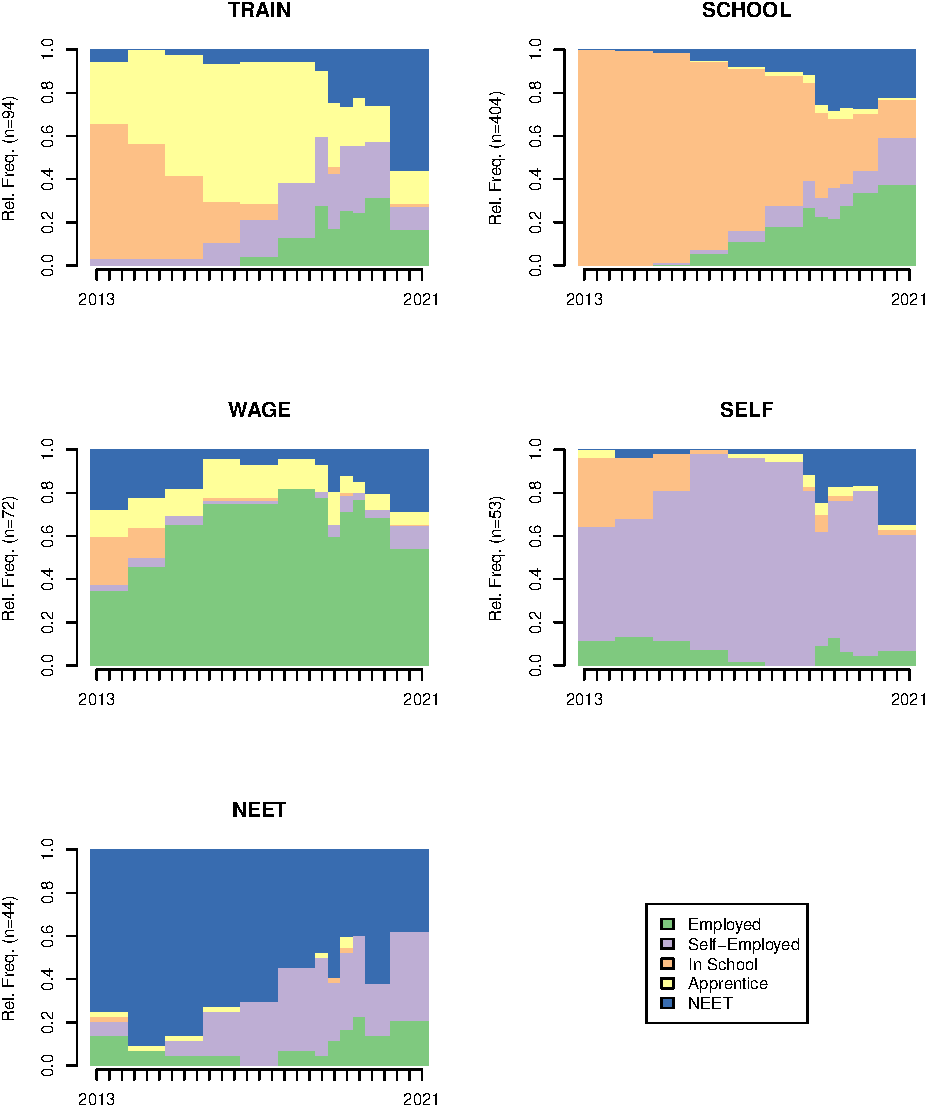
\includegraphics{figures/fig-clusters-1} \caption{Occupational status distribution plots by cluster}\label{fig:fig-clusters}
\end{figure}

Next, we employ Optimal Matching Analysis (OMA) to identify clusters of youth following similar paths during their school-to-work transition. OMA is a statistical technique that generates a measure of the similarity or difference between individual school-to-work transition sequences by comparing all pairs of sequences and performing insertions, deletions, or substitutions of single sequence elements to transform one sequence into the other (Elzinga, 2003). This method has been used to study early career patterns in Italy, Great Britain and West Germany (Scherer, 2001, 2005), the occupation career paths of Swedish women (Huang and Sverke, 2007), and the SWT of German youth (Achatz et al., 2022).

In optimal matching analysis, the cost of making a change to a sequence of states is typically measured using three types of costs: insertion, deletion, and substitution. Insertion/deletion cost is the cost of adding a new item to the sequence or removing an existing one, respectively. Substitution cost is the cost of replacing one item in the sequence with another item. Optimal matching algorithms seek to minimize the total cost of making changes to a sequence of items by choosing the combination of insertions, deletions, and substitutions that result in the lowest total cost, which serves as a measure of similarity between sequences. The distance matrix generated from this process is used in a hierarchical cluster analysis to group similar sequences into clusters. This is achieved by minimizing within-group differences and maximizing between-group differences, using Ward's fusion algorithm (Achatz et al., 2022; Dlouhy and Biemann, 2015). We use an insertion/deletion cost of 1 and a substitution cost matrix based on observed transition rates, which allows us to control for the likelihood of transitions occurring within the data {[}cite xx{]}. The TraMineR package in R (Gabadinho et al., 2011) was used to perform the analysis. We then use the R package WeightedCluster (Studer, 2013) to compute various clustering quality measures to determine the optimal number of clusters.

Descriptive statistics for each cluster are shown in Table \ref{tab:tbl-clustertbl} above, and Figure \ref{fig:fig-clusters} in the Appendix plots the status distribution by year for the five identified clusters. The first cluster, which we label ``TRAIN'', is primarily comprised of youth who participated in apprenticeship training in the years leading up to the baseline survey. Youth begin to transition into wage employment, self-employment, or inactivity in roughly equal proportions in around 2018, with a considerable proportion shifting to inactivity at endline. As apprenticeship training is generally considered to be a reliable route to (informal sector) employment, this shift to inactivity is concerning and may be of interest to policy makers. The youth in this cluster completed about 9 years of school, with the majority dropping out before completing junior high school.

The second cluster, which we call SCHOOL, accounts for about three-fifths of the sample with 404 youth, and is dominated by formal education, especially in the period leading up to the baseline survey. The state transition plot in Figure \ref{fig:fig-clusters} suggests that the extended schooling in this group (14.9 years on average, by far the most of any cluster) does increase the probability of finding employment, as this cluster exhibits the lowest rate of inactivity at endline. This cluster is characterised by the relatively low marriage and childbearing rates of the youth and the high educational level of the parents of the youth in the cluster.

\textbf{Table \ref{tab:tbl-clustertbl} indicates that this cluster completed their apprenticeships at a relatively advanced age -- around the age of 22 years and 6 months -- contradicting the intuitive assumption that apprentices enter the labor market sooner than youth who stay in formal schooling.}

The third cluster, WAGE, is comprised of 72 youth who are primarily engaged in wage employment over the observed period. Figure \ref{fig:fig-clusters} shows that most of these youth had completed their formal education by 2014 and enjoyed fairly stable employment throughout -- with a small proportion transitioning to inactivity at the tail end of the period, perhaps as a result of worsening economic conditions during the pandemic. The WAGE cluster contains a latent proportion of youth in apprenticeship training, possibly suggesting that completing an apprenticeship and finding wage employment is a solid predictor of job stability. We also note that there is very little transition between wage employment and self-employment in this cluster.

The fourth, SELF, is a relatively small cluster grouping together sequences of sustained self-employment from the beginning of the observed period or transitions from schooling to self-employment prior to 2016. This is the most homogeneous cluster, with essentially only two states observed after 2015: self-employment and NEET. In this cluster, youth only begin appearing as ``NEET'' at the start of the panel survey. As this data is more frequent and more granular than the event history data, we can infer that youth had described their past annual activity as self-employed may have in fact experienced stretches of inactivity within those years. This may be an important consideration when using a taxonomy that includes ``self-employment'' but relies on recall data for infrequent time intervals.

The final and smallest cluster, NEET, comprises youth who were inactive at the beginning of the observation period and began to transition into self-employment (and to a much smaller extend, wage employment) towards the endline. This cluster is the most unique in terms of its demographics: it contains almost exclusively young women (95\%) who dropped out very early (after only 6.7 years of schooling, on average -- compared to 12.8 for the sample), are married at a higher rate than the sample (59\% vs.~17\%) and have more children on average than the sample (1.73 vs.~0.53). These can be characterised as the ``stay-at-home-mothers'' - and the low educational attainment and low rates of transition to wage employment are concerning indicators for policy makers interested in gender equality in the region.

\hypertarget{labor-market-participants}{%
\subsubsection*{Labor Market Participants}\label{labor-market-participants}}

\singlespacing
\begin{table}[H]

\caption{\label{tab:tbl-employed}Youth Participating in Labor Market - Summary Statistics}
\centering
\begin{threeparttable}
\fontsize{8}{10}\selectfont
\begin{tabular}[t]{l>{\centering\arraybackslash}p{4em}>{\centering\arraybackslash}p{4em}>{\centering\arraybackslash}p{4em}>{\centering\arraybackslash}p{4em}>{\centering\arraybackslash}p{4em}>{\centering\arraybackslash}p{4em}>{\centering\arraybackslash}p{4em}}
\toprule
\textbf{Characteristic} & \textbf{Overall} & \textbf{Female} & \textbf{Male} & \textbf{19-21} & \textbf{22-24} & \textbf{25-27} & \textbf{28-30}\\
\midrule
N & 476 & 261 & 215 & 60 & 156 & 182 & 78\\
Formal employment & 11\% & 9.6\% & 13\% & 10\% & 7.1\% & 15\% & 13\%\\
Informal employment & 49\% & 43\% & 56\% & 43\% & 48\% & 49\% & 54\%\\
\cellcolor[HTML]{EEEEEE}{Working full time} & \cellcolor[HTML]{EEEEEE}{40\%} & \cellcolor[HTML]{EEEEEE}{35\%} & \cellcolor[HTML]{EEEEEE}{47\%} & \cellcolor[HTML]{EEEEEE}{28\%} & \cellcolor[HTML]{EEEEEE}{40\%} & \cellcolor[HTML]{EEEEEE}{42\%} & \cellcolor[HTML]{EEEEEE}{47\%}\\
\cellcolor[HTML]{EEEEEE}{Underemployed} & \cellcolor[HTML]{EEEEEE}{18\%} & \cellcolor[HTML]{EEEEEE}{17\%} & \cellcolor[HTML]{EEEEEE}{20\%} & \cellcolor[HTML]{EEEEEE}{22\%} & \cellcolor[HTML]{EEEEEE}{13\%} & \cellcolor[HTML]{EEEEEE}{20\%} & \cellcolor[HTML]{EEEEEE}{19\%}\\
Regular employment & 14\% & 15\% & 14\% & 13\% & 9.0\% & 18\% & 18\%\\
Casual worker & 19\% & 13\% & 27\% & 15\% & 20\% & 19\% & 19\%\\
\cellcolor[HTML]{EEEEEE}{Employer} & \cellcolor[HTML]{EEEEEE}{6.9\%} & \cellcolor[HTML]{EEEEEE}{3.8\%} & \cellcolor[HTML]{EEEEEE}{11\%} & \cellcolor[HTML]{EEEEEE}{5.0\%} & \cellcolor[HTML]{EEEEEE}{7.1\%} & \cellcolor[HTML]{EEEEEE}{7.1\%} & \cellcolor[HTML]{EEEEEE}{7.7\%}\\
\cellcolor[HTML]{EEEEEE}{Independent} & \cellcolor[HTML]{EEEEEE}{18\%} & \cellcolor[HTML]{EEEEEE}{20\%} & \cellcolor[HTML]{EEEEEE}{16\%} & \cellcolor[HTML]{EEEEEE}{18\%} & \cellcolor[HTML]{EEEEEE}{18\%} & \cellcolor[HTML]{EEEEEE}{18\%} & \cellcolor[HTML]{EEEEEE}{19\%}\\
Unemployed, looking for work & 40\% & 47\% & 31\% & 47\% & 45\% & 36\% & 33\%\\
Wage (of wage employed) &  &  &  &  &  &  & \\
\hspace{1em}<35,000 FCFA & 28\% & 32\% & 25\% & 40\% & 29\% & 29\% & 20\%\\
\hspace{1em}35,000-54,999 FCFA & 38\% & 39\% & 38\% & 30\% & 46\% & 38\% & 30\%\\
\hspace{1em}55,000-149.999 FCFA & 30\% & 26\% & 34\% & 30\% & 21\% & 29\% & 45\%\\
\hspace{1em}>150,000 FCFA & 3.6\% & 3.5\% & 3.8\% & 0\% & 3.6\% & 3.8\% & 5.0\%\\
Profits (of self-employed) &  &  &  &  &  &  & \\
\hspace{1em}<20,000 FCFA & 56\% & 67\% & 44\% & 71\% & 42\% & 61\% & 53\%\\
\hspace{1em}20,000-39,999 FCFA & 19\% & 20\% & 19\% & 21\% & 19\% & 14\% & 32\%\\
\hspace{1em}40,000-124.999 FCFA & 21\% & 13\% & 30\% & 7.1\% & 35\% & 18\% & 16\%\\
\hspace{1em}>125,000 FCFA & 3.7\% & 0\% & 7.4\% & 0\% & 3.2\% & 6.8\% & 0\%\\
Wealth index quintile & 3.05 & 2.97 & 3.16 &  &  &  & \\
Job Satisfaction (of wage and self-employed)¹ & 3.55 & 3.47 & 3.63 & 3.44 & 3.47 & 3.62 & 3.62\\
Life satisfaction¹ & 3.42 & 3.38 & 3.48 & 3.33 & 3.33 & 3.53 & 3.45\\
Where do you see yourself in five years? &  &  &  &  &  &  & \\
\hspace{1em}Still looking for work (NEET only) & 0.8\% & 1.1\% & 0.5\% & 0\% & 0.6\% & 1.1\% & 1.3\%\\
\hspace{1em}Working for same employer (wage employed only) & 4.0\% & 3.8\% & 4.2\% & 0\% & 2.6\% & 6.6\% & 3.8\%\\
\hspace{1em}Different/new employer & 28\% & 28\% & 29\% & 28\% & 35\% & 24\% & 23\%\\
\hspace{1em}(Still) self-employed & 57\% & 57\% & 56\% & 52\% & 51\% & 59\% & 67\%\\
\hspace{1em}In education/training & 5.5\% & 5.0\% & 6.1\% & 10\% & 7.7\% & 2.7\% & 3.8\%\\
\hspace{1em}Other & 5.1\% & 5.4\% & 4.7\% & 10\% & 3.2\% & 6.6\% & 1.3\%\\
\bottomrule
\end{tabular}
\begin{tablenotes}
\item Calculated using responses from baseline survey.
\item[1] Likert scale, 1 = Very dissatisfied, 5 = Very satisfied.
\end{tablenotes}
\end{threeparttable}
\end{table}
\doublespacing

Table \ref{tab:tbl-aspirations} tabulates the responses of self-employed, wage employed, and NEET youth to the question, ``What do you see yourself doing in five years?'' More employed youth envision themselves starting their own business than working for their current or a different employer. Moreover, wage workers reported the lowest levels of satisfaction with their current activity. Thus, despite its common characterization as the ``ideal'' employment situation, wage employment appears to be neither inherently stable nor particularly satisfactory --- at least in the early stages of a career. On the other hand, over a quarter of the self-employed expect to be working for an employer in five years, suggesting that many youth do not see self-employment as an absorbing state, either, but rather an intermediate step on the way to wage employment. In sum, youth expect to be in substantial flux between self- and wage employment, though a higher fraction of youth expect to be in self-employment in five years than to be employed for a wage.

When asked where they see themselves in 5 years, NEET youth were decidedly optimistic. Table \ref{tab:tbl-aspirations} shows that only 3 percent expected to still be searching for work and over 90 percent envisaged themselves working either for themselves or an employer. The majority (70 percent) of youth in this category saw themselves running their own business. The rate of NEET youth who foresee themselves working in a wage job (24 percent) is almost double the actual wage-employed rate observed in our regional census (11.7\%), however - despite this subgroup having completed less schooling than wage-employed youth on average. Within NEET, it is also possible to differentiate between active job-seekers and the inactive - those youth who have given up on looking for work. Four out of five NEET youth in the sample reported actively looking for a job at the time of the baseline survey; 74 percent of the inactive are young women who also dominated the INACTIVE cluster in the OMA analysis above. Over two thirds of youth who were NEET at baseline also reported never having been employed, and nearly half had been out of work for over six months at the time of the interview. Young job-seekers blame weak labor market demand and their own inadequate skills for their difficulties in securing employment. A shortage of employer demand and their own lack of work experience and training represent the most commonly listed difficulties: at least one of these being mentioned by 148 of 257 youth (58\%) in the subsample. 26\% said they did not know where to look, while 16\% cited unsatisfactory working conditions or unacceptably low wages offered at available jobs. Among those responding ``other'', many elaborated on the above categories (e.g., ``No jobs in political science''), pointed to their lack of means or connections, or were unable to identify any obstacles at all; three women listed maternity.

\hypertarget{survey-conclusion}{%
\section{Conclusion}\label{survey-conclusion}}

This paper studies the dynamics of the school-to-work transition for 752 youth aged 20-29 from urban Cotonou, Benin. A unique panel is created using mobile phone surveys; in each survey round, youth are classified into one of five groups reflecting their primary activity.

We combine reported activity history data with our panel to approximate the age of graduation and the duration of transition to the first job for each youth. In addition, we estimate transition intensity matrices and sequence analysis to describe common paths along the SWT. Finally, we discuss the impact of specific activity transitions on youth life satisfaction and the reported aspirations of youth, and the obstacles they face on the labor market.

The SWT is observed for about 68 percent of the sample, with the majority reporting a transition to wage work or self-employment in the period directly following their final year of schooling or training. Youth who enter the labor market as self-employed tend to be less educated and have parents with lower educational attainment than youth who enter the labor market as wage-employed or unemployed. Youth who do not find work in the first period after graduation wait less than a year, on average, before entering either wage or self-employment. Youth who complete university education (master's level or higher) take about six months longer to find their first job, though education up to secondary schooling does not appear to extend the duration.

Using a combination of retrospective employment history and panel data to calculate average ages of transition, we find that youth in Cotonou graduate at the age of 22 years, seven months, and find their first employment exactly a year later, on average. If the transition duration calculated for this sample were representative of the nation, it would rank Benin as a country with one of the shortest transitions to work in the world. However, given the higher availability of non-agricultural informal work in urban areas, one expects the transition speed to be shorter in urban Cotonou than in the rest of the country.

transition intensity matrices suggest that wage employment and self-employment are stable relative to inactivity, meaning youth in employment are more likely to stay in the same type of employment than NEET youth are likely to stay inactive. However, higher rates of transition are observed for the (approximately quarterly) panel data than in yearly historical data, suggesting that annual data often used for studying the SWT may hide significant turbulence in employment status. There are relatively few transitions into regular work (with a single employer) from self-employment, schooling or inactivity, suggesting that a period of casual employment usually precedes a more stable employment relationship.

We also use optimal matching analysis to identify clusters of youth following similar transition paths. The five identified clusters reflect the five activity types used, reflecting the relative stability of states. However, youth whose paths are dominated by inactivity are shown to be almost exclusively young women with lower educational attainment and larger families.

Finally, we find that youth expect to be self-employed, not employed, even when in wage employment. This stands in contrast to the high stability of wage employed observed in the panel data.

Panel data is a useful tool for examining the dynamics of the transition process, such as how quickly young people enter the labor market, what types of jobs they obtain, and how their employment prospects change over time. Panel data can also be used to analyze the impact of different factors on the transition process, such as the quality of education, the availability of job opportunities, or the effects of policy interventions. By using panel data, researchers can gain a more nuanced and detailed understanding of the school-to-work transition in Africa, and can identify potential areas for improvement in policy and practice.

We make a unique contribution to the literature by estimating the effects of transition on youth well-being. We find that while youth who have transitioned to steady employment are more satisfied with their lives, none of the specific transitions examined, e.g.~the transition from wage to self-employment, appear to have an effect on youth satisfaction. Finally, we show that mobile phone data collection are promising for tracking labor market performance, despite moderate attrition; however, we observed higher response to the in-person baseline and endline waves, despite these being more time-consuming than the follow-up surveys. Thus, while urban youth are an ideal subject for phone-based surveys due to their high literacy and relatively high phone ownership and high network coverage in cities, incentives for increasing response and reducing survey fatigue in longitudinal remote studies remains an important topic of research. On the balance, however, we agree that ``the cost savings of a phone survey are substantial, as long as the questions of interest call for high frequency panel data'' (Dillon 2012).

\newpage

\hypertarget{references}{%
\section*{References}\label{references}}
\addcontentsline{toc}{section}{References}

\noindent

\hypertarget{refs}{}
\begin{CSLReferences}{1}{0}
\leavevmode\vadjust pre{\hypertarget{ref-achatz2022}{}}%
Achatz, J., Jahn, K., and Schels, B. (2022). On the non-standard routes: Vocational training measures in the school-to-work transitions of lower-qualified youth in {Germany}. \emph{Journal of Vocational Education \& Training}, \emph{74}(2), 289--310. \url{https://doi.org/10.1080/13636820.2020.1760335}

\leavevmode\vadjust pre{\hypertarget{ref-africandevelopmentbank2016}{}}%
African Development Bank. (2016). \emph{Jobs for {Youth} in {Africa}: {Strategy} for {Creating} 25 {Million Jobs} and {Equipping} 50 {Million Youth} 2016-2025}. {African Development Bank}.

\leavevmode\vadjust pre{\hypertarget{ref-arulampalam2001}{}}%
Arulampalam, W. (2001). Is {Unemployment Really Scarring}? {Effects} of {Unemployment Experiences} on {Wages}. \emph{The Economic Journal}, \emph{111}(475), F585--F606. \url{https://doi.org/10.1111/1468-0297.00664}

\leavevmode\vadjust pre{\hypertarget{ref-bandara2019}{}}%
Bandara, A. (2019). Youth labor market expectations and job matching in sub-{Saharan Africa}: Evidence from school-to-work transition surveys. \emph{Applied Economics}, \emph{51}(8), 762--780. \url{https://doi.org/10.1080/00036846.2018.1512742}

\leavevmode\vadjust pre{\hypertarget{ref-barro2013}{}}%
Barro, R. J., and Lee, J. W. (2013). A {New Data Set} of {Educational Attainment} in the {World}, 1950\textendash{} 2010. \emph{Journal of Development Economics}, \emph{104}, 184--198. \url{https://doi.org/10.1016/j.jdeveco.2012.10.001}

\leavevmode\vadjust pre{\hypertarget{ref-benhassine2018}{}}%
Benhassine, N., McKenzie, D., Pouliquen, V., and Santini, M. (2018). Does {Inducing Informal Firms} to {Formalize Make Sense}? {Experimental Evidence} from {Benin}. \emph{Journal of Public Economics}, \emph{157}, 1--14. \url{https://doi.org/10.1016/j.jpubeco.2017.11.004}

\leavevmode\vadjust pre{\hypertarget{ref-bosch2007}{}}%
Bosch, M., and Maloney, W. (2007). \emph{Comparative {Analysis} of {Labor Market Dynamics Using Markov Processes}: {An Application} to {Informality}} (World \{\{Bank Policy Research Working Paper\}\} No. 4429). {World Bank}.

\leavevmode\vadjust pre{\hypertarget{ref-bosch2010}{}}%
Bosch, M., and Maloney, W. F. (2010). Comparative analysis of labor market dynamics using {Markov} processes: {An} application to informality. \emph{Labour Economics}, \emph{17}(4), 621--631. \url{https://doi.org/10.1016/j.labeco.2010.01.005}

\leavevmode\vadjust pre{\hypertarget{ref-bowers1998}{}}%
Bowers, N. (1998). Getting {Started}, {Settling} in: {The Transition} from {Education} to the {Labour Market}. In OECD (Ed.), \emph{1998 {Employment Outlook}}.

\leavevmode\vadjust pre{\hypertarget{ref-bridges2017}{}}%
Bridges, S., Fox, L., Gaggero, A., and Owens, T. (2017). Youth {Unemployment} and {Earnings} in {Africa}: {Evidence} from {Tanzanian Retrospective Data}. \emph{Journal of African Economies}, \emph{26}(2). \url{https://doi.org/10.1093/jae/ejw020}

\leavevmode\vadjust pre{\hypertarget{ref-calves2013}{}}%
Calvès, A. E., Kobiané, J.-F., and N'Bouké, A. (2013). Privatization of {Education} and {Labor Force Inequality} in {Urban Francophone Africa}: {The Transition} from {School} to {Work} in {Ouagadougou}. \emph{World Development}, \emph{47}, 136--148. \url{https://doi.org/10.1016/j.worlddev.2013.03.001}

\leavevmode\vadjust pre{\hypertarget{ref-cockx2012}{}}%
Cockx, B., and Picchio, M. (2012). Scarring effects of remaining unemployed for long-term unemployed school-leavers. \emph{Journal of the Royal Statistical Society: Series A (Statistics in Society)}, \emph{176}(4), 951--980. \url{https://doi.org/10.1111/j.1467-985x.2012.01086.x}

\leavevmode\vadjust pre{\hypertarget{ref-cunningham2011}{}}%
Cunningham, W., and Salvagno, J. B. (2011). \emph{Youth {Employment Transitions} in {Latin America}}. {The World Bank}. \url{https://doi.org/10.1596/1813-9450-5521}

\leavevmode\vadjust pre{\hypertarget{ref-dedehouanou2019}{}}%
Dedehouanou, S. F. A., Tiberti, L., Houeninvo, H., and Monwanou, D. I. (2019). Working while {Studying}: {Employment Premium} or {Penalty} for {Youth} in {Benin}? \emph{SSRN Electronic Journal}. \url{https://doi.org/10.2139/ssrn.3344584}

\leavevmode\vadjust pre{\hypertarget{ref-demombynes2013}{}}%
Demombynes, G., Gubbins, P., and Romeo, A. (2013). \emph{Challenges and {Opportunities} of {Mobile Phone-Based Data Collection}: {Evidence} from {South Sudan}} (World \{\{Bank Policy Research Working Paper\}\} No. 6321). {World Bank}. \url{https://doi.org/10.1596/1813-9450-6321}

\leavevmode\vadjust pre{\hypertarget{ref-dlouhy2015}{}}%
Dlouhy, K., and Biemann, T. (2015). Optimal matching analysis in career research: {A} review and some best-practice recommendations. \emph{Journal of Vocational Behavior}, \emph{90}, 163--173. \url{https://doi.org/10.1016/j.jvb.2015.04.005}

\leavevmode\vadjust pre{\hypertarget{ref-egel2010}{}}%
Egel, D., and Salehi-Isfahani, D. (2010). Youth {Transitions} to {Employment} and {Marriage} in {Iran}: {Evidence} from the {School} to {Work Transition Survey}. \emph{Middle East Development Journal}, \emph{2}(1), 89--120. \url{https://doi.org/10.1142/S1793812010000198}

\leavevmode\vadjust pre{\hypertarget{ref-elzinga2003}{}}%
Elzinga, C. H. (2003). Sequence {Similarity}: {A Nonaligning Technique}. \emph{Sociological Methods \& Research}, \emph{32}(1), 3--29. \url{https://doi.org/10.1177/0049124103253373}

\leavevmode\vadjust pre{\hypertarget{ref-emmenegger2017}{}}%
Emmenegger, P., Marx, P., and Schraff, D. (2017). Off to a {Bad Start}: {Unemployment} and {Political Interest} during {Early Adulthood}. \emph{The Journal of Politics}, \emph{79}(1), 315--328. \url{https://doi.org/10.1086/688226}

\leavevmode\vadjust pre{\hypertarget{ref-fox2020}{}}%
Fox, L., Mader, P., Sumberg, J., Flynn, J., and Oosterom, M. (2020). \emph{Africa's '{Youth Employment}' {Crisis Is Actually} a '{Missing Jobs}' {Crisis}}. {Brookings Institute}.

\leavevmode\vadjust pre{\hypertarget{ref-frazer2006}{}}%
Frazer, G. (2006). Learning the {Master}'s {Trade}: {Apprenticeship} and {Human Capital} in {Ghana}. \emph{Journal of Development Economics}, \emph{81}(2), 259--298.

\leavevmode\vadjust pre{\hypertarget{ref-gabadinho2011}{}}%
Gabadinho, A., Ritschard, G., Müller, N. S., and Studer, M. (2011). Analyzing and {Visualizing State Sequences} in {\emph{R}} with {\textbf{TraMineR}}. \emph{Journal of Statistical Software}, \emph{40}(4). \url{https://doi.org/10.18637/jss.v040.i04}

\leavevmode\vadjust pre{\hypertarget{ref-honwana2012}{}}%
Honwana, A. M. (2012). \emph{The {Time} of {Youth}: {Work}, {Social Change}, and {Politics} in {Africa}}. {Kumarian Press Pub}.

\leavevmode\vadjust pre{\hypertarget{ref-huang2007}{}}%
Huang, Q., and Sverke, M. (2007). Women's occupational career patterns over 27 years: {Relations} to family of origin, life careers, and wellness. \emph{Journal of Vocational Behavior}, \emph{70}(2), 369--397. \url{https://doi.org/10.1016/j.jvb.2006.12.003}

\leavevmode\vadjust pre{\hypertarget{ref-mains2011}{}}%
Mains, D. (2011). \emph{Hope {Is Cut}: {Youth}, {Unemployment}, and the {Future} in {Urban Ethiopia}}. {Temple University Press}.

\leavevmode\vadjust pre{\hypertarget{ref-manacorda2017}{}}%
Manacorda, M., Rosati, F. C., Ranzani, M., and Dachille, G. (2017). Pathways from {School} to {Work} in the {Developing World}. \emph{IZA Journal of Labor \& Development}, \emph{6}(1), 1. \url{https://doi.org/10.1186/s40175-016-0067-5}

\leavevmode\vadjust pre{\hypertarget{ref-matsumoto2010}{}}%
Matsumoto, M., Elder, S., International Labour Office, and Employment Policy Department. (2010). \emph{Characterizing the {School-to-Work Transitions} of {Young Men} and {Women}: {Evidence} from the {ILO School-to-Work Transition Surveys}}. {ILO}.

\leavevmode\vadjust pre{\hypertarget{ref-moller2015}{}}%
Möller, J., and Umkehrer, M. (2015). Are there {Long-Term Earnings Scars} from {Youth Unemployment} in {Germany}? \emph{Jahrbücher Für Nationalökonomie Und Statistik}, \emph{235}(4-5), 474--498. \url{https://doi.org/10.1515/jbnst-2015-4-509}

\leavevmode\vadjust pre{\hypertarget{ref-mroz2006}{}}%
Mroz, T. A., and Savage, T. H. (2006). The {Long-Term Effects} of {Youth Unemployment}. \emph{Journal of Human Resources}, \emph{XLI}(2), 259--293. \url{https://doi.org/10.3368/jhr.xli.2.259}

\leavevmode\vadjust pre{\hypertarget{ref-nilsson2019}{}}%
Nilsson, B. (2019). The {School-to-Work Transition} in {Developing Countries}. \emph{The Journal of Development Studies}, \emph{55}(5), 745--764. \url{https://doi.org/10.1080/00220388.2018.1475649}

\leavevmode\vadjust pre{\hypertarget{ref-nordman2015}{}}%
Nordman, C. J., and Pasquier-Doumer, L. (2015). Transitions in a {West African Labour Market}: {The Role} of {Family Networks}. \emph{Journal of Behavioral and Experimental Economics}, \emph{54}, 74--85. \url{https://doi.org/10.1016/j.socec.2014.11.008}

\leavevmode\vadjust pre{\hypertarget{ref-nordman2014}{}}%
Nordman, C. J., and Pasquier-Doumer, L. (2014). Vocational {Education}, on-the-{Job Training}, and {Labour Market Integration} of {Young Workers} in {Urban West Africa}. \emph{PROSPECTS}, \emph{44}(3), 445--462. \url{https://doi.org/10.1007/s11125-014-9320-3}

\leavevmode\vadjust pre{\hypertarget{ref-nordstromskans2011}{}}%
Nordström Skans, O. (2011). Scarring {Effects} of the {First Labor Market Experience}. \emph{SSRN Electronic Journal}. \url{https://doi.org/10.2139/ssrn.1790676}

\leavevmode\vadjust pre{\hypertarget{ref-quintini2007}{}}%
Quintini, G., Martin, J. P., and Martin, S. (2007). The {Changing Nature} of the {School-to-Work Transition Process} in {OECD Countries}. \emph{SSRN Electronic Journal}. \url{https://doi.org/10.2139/ssrn.1884070}

\leavevmode\vadjust pre{\hypertarget{ref-quintini2014}{}}%
Quintini, G., and Martin, S. (2014). \emph{Same {Same} but {Different}: {School-to-work Transitions} in {Emerging} and {Advanced Economies}} (\{\{OECD Social\}\}, \{\{Employment\}\} and \{\{Migration Working Papers\}\} No. 154; {OECD Social}, {Employment} and {Migration Working Papers}, Vol. 154). {OECD}. \url{https://doi.org/10.1787/5jzbb2t1rcwc-en}

\leavevmode\vadjust pre{\hypertarget{ref-scherer2001}{}}%
Scherer, S. (2001). Early {Career Patterns}: {A Comparison} of {Great Britain} and {West Germany}. \emph{European Sociological Review}, \emph{17}(2), 119--144. \url{https://doi.org/10.1093/esr/17.2.119}

\leavevmode\vadjust pre{\hypertarget{ref-scherer2005}{}}%
Scherer, S. (2005). Patterns of {Labour Market Entry} \textendash{} {Long Wait} or {Career Instability}? {An Empirical Comparison} of {Italy}, {Great Britain} and {West Germany}. \emph{European Sociological Review}, \emph{21}(5), 427--440. \url{https://doi.org/10.1093/esr/jci029}

\leavevmode\vadjust pre{\hypertarget{ref-schmillen2017}{}}%
Schmillen, A., and Umkehrer, M. (2017). The scars of youth: {Effects} of early-career unemployment on future unemployment experience. \emph{International Labour Review}, \emph{156}(3-4), 465--494. \url{https://doi.org/10.1111/ilr.12079}

\leavevmode\vadjust pre{\hypertarget{ref-studer2013}{}}%
Studer, M. (2013). \emph{{WeightedCluster Library Manual}: {A} practical guide to creating typologies of trajectories in the social sciences with {R}}. \url{https://doi.org/10.12682/LIVES.2296-1658.2013.24}

\leavevmode\vadjust pre{\hypertarget{ref-sumberg2021}{}}%
Sumberg, J., Fox, L., Flynn, J., Mader, P., and Oosterom, M. (2021). Africa's {``{Youth Employment}''} {Crisis Is Actually} a {``{Missing Jobs}''} {Crisis}. \emph{Development Policy Review}, \emph{39}(4), 621--643. \url{https://doi.org/10.1111/dpr.12528}

\leavevmode\vadjust pre{\hypertarget{ref-urdal2006}{}}%
Urdal, H. (2006). A {Clash} of {Generations}? {Youth Bulges} and {Political Violence}. \emph{International Studies Quarterly}, \emph{50}(3), 607--629. \url{https://doi.org/10.1111/j.1468-2478.2006.00416.x}

\end{CSLReferences}

\newpage

\hypertarget{survey-appendix-a}{%
\section*{Appendix A}\label{survey-appendix-a}}
\addcontentsline{toc}{section}{Appendix A}

\setcounter{figure}{0}
\renewcommand{\thefigure}{A\arabic{figure}}
\setcounter{table}{0}
\renewcommand{\thetable}{A\arabic{table}}

\hypertarget{survey-census}{%
\section*{Cotonou census}\label{survey-census}}

\begin{figure}[H] \caption{\label{fig:litt} Geographic Coverage of Survey}
\centering
\makebox[.8\textwidth][c]{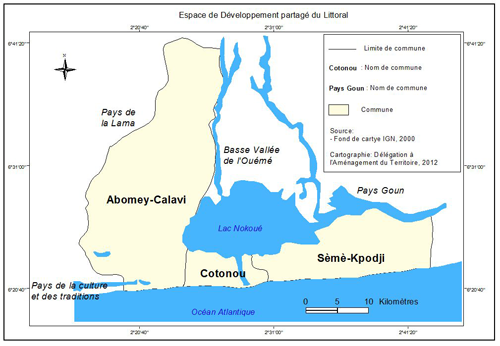
\includegraphics[width=.75\textwidth]{path/figures/littoral_carte}}
\end{figure}

\singlespacing

\providecommand{\docline}[3]{\noalign{\global\setlength{\arrayrulewidth}{#1}}\arrayrulecolor[HTML]{#2}\cline{#3}}

\setlength{\tabcolsep}{0pt}

\renewcommand*{\arraystretch}{1.5}

\begin{longtable}[c]{|p{1.00in}|p{0.80in}|p{0.80in}|p{0.80in}}

\caption{\textcolor[HTML]{000000}{\fontsize{11}{13}\selectfont{\global\setmainfont{Palatino}{Census\ of\ 13\ zones\ de\ dénombrement}}}}\label{tab:tbl-census}\\

\hhline{~~~~}

\multicolumn{1}{!{\color[HTML]{000000}\vrule width 0pt}>{\raggedright}p{\dimexpr 1in+0\tabcolsep+0\arrayrulewidth}}{\textcolor[HTML]{000000}{\fontsize{9}{9}\selectfont{\global\setmainfont{Palatino}{\ }}}} & \multicolumn{1}{!{\color[HTML]{000000}\vrule width 0pt}>{\raggedright}p{\dimexpr 0.8in+0\tabcolsep+0\arrayrulewidth}}{\textcolor[HTML]{000000}{\fontsize{9}{9}\selectfont{\global\setmainfont{Palatino}{Aged\ 15-19}}}} & \multicolumn{1}{!{\color[HTML]{000000}\vrule width 0pt}>{\raggedright}p{\dimexpr 0.8in+0\tabcolsep+0\arrayrulewidth}}{\textcolor[HTML]{000000}{\fontsize{9}{9}\selectfont{\global\setmainfont{Palatino}{Aged\ 20-29}}}} & \multicolumn{1}{!{\color[HTML]{000000}\vrule width 0pt}>{\raggedright}p{\dimexpr 0.8in+0\tabcolsep+0\arrayrulewidth}!{\color[HTML]{000000}\vrule width 0pt}}{\textcolor[HTML]{000000}{\fontsize{9}{9}\selectfont{\global\setmainfont{Palatino}{Aged\ 30\ and\ above}}}} \\

\hhline{>{\arrayrulecolor[HTML]{666666}\global\arrayrulewidth=2pt}->{\arrayrulecolor[HTML]{666666}\global\arrayrulewidth=2pt}->{\arrayrulecolor[HTML]{666666}\global\arrayrulewidth=2pt}->{\arrayrulecolor[HTML]{666666}\global\arrayrulewidth=2pt}-}\endhead



\multicolumn{4}{!{\color[HTML]{FFFFFF}\vrule width 0pt}>{\raggedright}p{\dimexpr 3.4in+6\tabcolsep+3\arrayrulewidth}!{\color[HTML]{FFFFFF}\vrule width 0pt}}{\textcolor[HTML]{000000}{\fontsize{9}{9}\selectfont{\global\setmainfont{Palatino}{n,\ \%.}}}} \\

\endfoot



\multicolumn{1}{!{\color[HTML]{000000}\vrule width 0pt}>{\raggedright}p{\dimexpr 1in+0\tabcolsep+0\arrayrulewidth}}{\textcolor[HTML]{000000}{\fontsize{9}{9}\selectfont{\global\setmainfont{Palatino}{}}}} & \multicolumn{1}{!{\color[HTML]{000000}\vrule width 0pt}>{\raggedright}p{\dimexpr 0.8in+0\tabcolsep+0\arrayrulewidth}}{\textcolor[HTML]{000000}{\fontsize{9}{9}\selectfont{\global\setmainfont{Palatino}{1417\ (71.64)}}}} & \multicolumn{1}{!{\color[HTML]{000000}\vrule width 0pt}>{\raggedright}p{\dimexpr 0.8in+0\tabcolsep+0\arrayrulewidth}}{\textcolor[HTML]{000000}{\fontsize{9}{9}\selectfont{\global\setmainfont{Palatino}{1144\ (31.07)}}}} & \multicolumn{1}{!{\color[HTML]{000000}\vrule width 0pt}>{\raggedright}p{\dimexpr 0.8in+0\tabcolsep+0\arrayrulewidth}!{\color[HTML]{000000}\vrule width 0pt}}{\textcolor[HTML]{000000}{\fontsize{9}{9}\selectfont{\global\setmainfont{Palatino}{87\ (1.35)}}}} \\





\multicolumn{1}{!{\color[HTML]{000000}\vrule width 0pt}>{\raggedright}p{\dimexpr 1in+0\tabcolsep+0\arrayrulewidth}}{\textcolor[HTML]{000000}{\fontsize{9}{9}\selectfont{\global\setmainfont{Palatino}{In\ School}}}} & \multicolumn{1}{!{\color[HTML]{000000}\vrule width 0pt}>{\raggedright}p{\dimexpr 0.8in+0\tabcolsep+0\arrayrulewidth}}{\textcolor[HTML]{000000}{\fontsize{9}{9}\selectfont{\global\setmainfont{Palatino}{125\ (6.32)}}}} & \multicolumn{1}{!{\color[HTML]{000000}\vrule width 0pt}>{\raggedright}p{\dimexpr 0.8in+0\tabcolsep+0\arrayrulewidth}}{\textcolor[HTML]{000000}{\fontsize{9}{9}\selectfont{\global\setmainfont{Palatino}{635\ (17.25)\ }}}} & \multicolumn{1}{!{\color[HTML]{000000}\vrule width 0pt}>{\raggedright}p{\dimexpr 0.8in+0\tabcolsep+0\arrayrulewidth}!{\color[HTML]{000000}\vrule width 0pt}}{\textcolor[HTML]{000000}{\fontsize{9}{9}\selectfont{\global\setmainfont{Palatino}{574\ (24.35)}}}} \\





\multicolumn{1}{!{\color[HTML]{000000}\vrule width 0pt}>{\raggedright}p{\dimexpr 1in+0\tabcolsep+0\arrayrulewidth}}{\textcolor[HTML]{000000}{\fontsize{9}{9}\selectfont{\global\setmainfont{Palatino}{Other}}}} & \multicolumn{1}{!{\color[HTML]{000000}\vrule width 0pt}>{\raggedright}p{\dimexpr 0.8in+0\tabcolsep+0\arrayrulewidth}}{\textcolor[HTML]{000000}{\fontsize{9}{9}\selectfont{\global\setmainfont{Palatino}{95\ (4.80)}}}} & \multicolumn{1}{!{\color[HTML]{000000}\vrule width 0pt}>{\raggedright}p{\dimexpr 0.8in+0\tabcolsep+0\arrayrulewidth}}{\textcolor[HTML]{000000}{\fontsize{9}{9}\selectfont{\global\setmainfont{Palatino}{1183\ (32.13)\ }}}} & \multicolumn{1}{!{\color[HTML]{000000}\vrule width 0pt}>{\raggedright}p{\dimexpr 0.8in+0\tabcolsep+0\arrayrulewidth}!{\color[HTML]{000000}\vrule width 0pt}}{\textcolor[HTML]{000000}{\fontsize{9}{9}\selectfont{\global\setmainfont{Palatino}{664\ (56.68)}}}} \\





\multicolumn{1}{!{\color[HTML]{000000}\vrule width 0pt}>{\raggedright}p{\dimexpr 1in+0\tabcolsep+0\arrayrulewidth}}{\textcolor[HTML]{000000}{\fontsize{9}{9}\selectfont{\global\setmainfont{Palatino}{Self-Employed}}}} & \multicolumn{1}{!{\color[HTML]{000000}\vrule width 0pt}>{\raggedright}p{\dimexpr 0.8in+0\tabcolsep+0\arrayrulewidth}}{\textcolor[HTML]{000000}{\fontsize{9}{9}\selectfont{\global\setmainfont{Palatino}{35\ (1.77)}}}} & \multicolumn{1}{!{\color[HTML]{000000}\vrule width 0pt}>{\raggedright}p{\dimexpr 0.8in+0\tabcolsep+0\arrayrulewidth}}{\textcolor[HTML]{000000}{\fontsize{9}{9}\selectfont{\global\setmainfont{Palatino}{33\ (11.76)}}}} & \multicolumn{1}{!{\color[HTML]{000000}\vrule width 0pt}>{\raggedright}p{\dimexpr 0.8in+0\tabcolsep+0\arrayrulewidth}!{\color[HTML]{000000}\vrule width 0pt}}{\textcolor[HTML]{000000}{\fontsize{9}{9}\selectfont{\global\setmainfont{Palatino}{117\ (17.28)}}}} \\





\multicolumn{1}{!{\color[HTML]{000000}\vrule width 0pt}>{\raggedright}p{\dimexpr 1in+0\tabcolsep+0\arrayrulewidth}}{\textcolor[HTML]{000000}{\fontsize{9}{9}\selectfont{\global\setmainfont{Palatino}{Employed}}}} & \multicolumn{1}{!{\color[HTML]{000000}\vrule width 0pt}>{\raggedright}p{\dimexpr 0.8in+0\tabcolsep+0\arrayrulewidth}}{\textcolor[HTML]{000000}{\fontsize{9}{9}\selectfont{\global\setmainfont{Palatino}{306\ (15.47)}}}} & \multicolumn{1}{!{\color[HTML]{000000}\vrule width 0pt}>{\raggedright}p{\dimexpr 0.8in+0\tabcolsep+0\arrayrulewidth}}{\textcolor[HTML]{000000}{\fontsize{9}{9}\selectfont{\global\setmainfont{Palatino}{\ 287\ (7.79)}}}} & \multicolumn{1}{!{\color[HTML]{000000}\vrule width 0pt}>{\raggedright}p{\dimexpr 0.8in+0\tabcolsep+0\arrayrulewidth}!{\color[HTML]{000000}\vrule width 0pt}}{\textcolor[HTML]{000000}{\fontsize{9}{9}\selectfont{\global\setmainfont{Palatino}{22\ (0.34)}}}} \\





\multicolumn{1}{!{\color[HTML]{000000}\vrule width 0pt}>{\raggedright}p{\dimexpr 1in+0\tabcolsep+0\arrayrulewidth}}{\textcolor[HTML]{000000}{\fontsize{9}{9}\selectfont{\global\setmainfont{Palatino}{Apprentice}}}} & \multicolumn{1}{!{\color[HTML]{000000}\vrule width 0pt}>{\raggedright}p{\dimexpr 0.8in+0\tabcolsep+0\arrayrulewidth}}{\textcolor[HTML]{000000}{\fontsize{9}{9}\selectfont{\global\setmainfont{Palatino}{1978\ (100.00)}}}} & \multicolumn{1}{!{\color[HTML]{000000}\vrule width 0pt}>{\raggedright}p{\dimexpr 0.8in+0\tabcolsep+0\arrayrulewidth}}{\textcolor[HTML]{000000}{\fontsize{9}{9}\selectfont{\global\setmainfont{Palatino}{3682\ (100.00)}}}} & \multicolumn{1}{!{\color[HTML]{000000}\vrule width 0pt}>{\raggedright}p{\dimexpr 0.8in+0\tabcolsep+0\arrayrulewidth}!{\color[HTML]{000000}\vrule width 0pt}}{\textcolor[HTML]{000000}{\fontsize{9}{9}\selectfont{\global\setmainfont{Palatino}{6464\ (100.00)}}}} \\

\hhline{>{\arrayrulecolor[HTML]{666666}\global\arrayrulewidth=2pt}->{\arrayrulecolor[HTML]{666666}\global\arrayrulewidth=2pt}->{\arrayrulecolor[HTML]{666666}\global\arrayrulewidth=2pt}->{\arrayrulecolor[HTML]{666666}\global\arrayrulewidth=2pt}-}



\end{longtable}

\doublespacing

\newpage

\hypertarget{survey-weighting}{%
\section*{Sampling and weighting}\label{survey-weighting}}

Cluster sampling was used to select the 752 youth interviewed in the face-to-face baseline survey. The twelve \emph{départements} of Benin are subdivided into 77 \emph{communes}, which are further subdivided into \emph{arrondissements}. To delimit the geographic area for the census, we first manually selected five \emph{arrondissements} from the three \emph{communes} which constitute the Cotonou metropolitan area (Figure \ref{fig:litt}). The five \emph{arrondissements} were chosen in consultation with survey partners experienced in data collection in the region to be as representative of urban Cotonou as possible.

In a second step, 15 Zones de dénombrement (ZDs) -- the smallest administrative divisions in Benin -- were selected from the five \emph{arrondissements} (or clusters) and constitute the primary sampling unit (PSU) of the sample. The number of ZDs chosen per cluster was proportional to the size of the youth population in each \emph{arrondissement} at the time of the 2016 census, such that each household in the five \emph{arrondissements} still had an equally likely chance of being sampled and no reweighting was necessary. Eight ZDs were thus drawn from the \emph{arrondissement} of Cotonou, two from Godomey, two from Calavi, one from Agbanglandan, and one from Ekpè.

All 4,905 households living in within the boundaries of these 15 ZDs were interviewed in person to ascertain the age and employment status (in school, in apprenticeship, employed, self-employed, or inactive) of all household members. Table \ref{tab:tbl-census} in the Appendix shows that a total of 19,032 individuals were covered by the census, with all individuals aged 20-29 in these households (excluding apprentices, due to overlap with a second study by the author\footnote{A number of apprentices appear in the final sample due to misreporting or a change in activity between the time of the census and the baseline interview.}) constituting the sample frame for the panel survey. Survey participants were selected randomly from this pool of 3,395 youth; the survey is thus representative of youth aged 20-29 in the metropolitan area of Cotonou whose primary economic activity is not apprenticeship training.

\newpage

\hypertarget{survey-transitions}{%
\section*{Studying transitions as a continuous Markov processes}\label{survey-transitions}}

In Appendix B, we depict transitions between \(K\) states employment states as transition intensity matrices. Each cell of the transition intensity matrix is given by the probability of transitioning from an initial employment state \(i\) to a subsequent employment state \(j\), which is simply given by \(p_{ij} = n_{ij}/n_i\), such that the matrices in Appendix B can be depicted as

\singlespacing

\[
Q= \begin{pmatrix}
p_{11} & \dots & p_{1k}\\
\vdots & \ddots & \vdots \\
p_{k1} &\dots & p_{kk} \\
\end{pmatrix}
\]
\doublespacing

where \(n_{ij}\) is the number of youth making the transition from state \(i\) to \(j\) and \(n_i\) is the number of youth in the initial state \(i\).

Transition intensity matrices alone do not allow us to make informative comparisons between subgroups, as we do not know if a higher \(p_{ij}\) indicates a preference of a subgroup for a certain transition, or simply higher turnover. To mitigate this issue, we follow Bosch and Maloney (2007) and Cunningham and Salvagno (2011) in decomposing the transition intensity matrices into two separate elements, which allow us to infer the propensity at which groups make certain transitions independent of that group's likelihood to change states.

``Since we have access to discrete panel data, rather than continuous time data, equation (1) can be interpreted as the transition probability if we assume that the discrete-time mobility process captured by our data is generated by a continuous-time homogenous Markov process. In other words, if we assume that transitions between states occur at random points in time, then a random draw of a transition in one point in time has the same probability (within a confidence interval) of a draw at any other point in time.''

This rate of transition, which can be referred to as intensities (Bosch and Maloney, 2007), make differences across different groups (age groups or gender) difficult because they do not account for the likelihood of separation (i.e.~changing states). For example, younger individuals are much less likely to transition out of school; thus, the rate of transition from school to, say, wage employment will be deflated relative to older youth around graduation age, and will tell us little about the preference of younger school-leavers for wage employment relative to other options.

The method proposed by Bosch and Maloney (2007) and Bosch and Maloney (2010) and applied to youth transitions by Cunningham and Salvagno (2011) controls for the likelihood of separation by
factoring \(Q\) into two elements, the rate of separation and the propensity to move, denoted by \(Q = \lambda(M-I)\):

\singlespacing

\[
Q= \begin{pmatrix}
-p_{11} &  &  &  \\
 & \ddots &  &  \\
 &   & -p_{kk} & \\
\end{pmatrix}
\begin{pmatrix} \begin{bmatrix}
0 &  r_{ij} & \\
 & \ddots &  \\
 &  & 0  \\
\end{bmatrix} - I
\end{pmatrix}
\]
\doublespacing

where \(r_{ij} = -p_{ij}/p_{ii}\) for \(i \neq j\) and \(i = 1, \dots, K\) and \(I\) is the identity matrix.

The first component represents the transition probabilities independent of the rate at which different age groups leave any sector, and is called the propensity matrix. The second is the rate of transition, and is referred to as the rate of separation matrix. By decomposing the transition intensity matrix into the propensity matrix and the rate of separation matrix, we can determine if movements to employment states observed in the transition intensity matrix are reflecting greater entry of certain age groups into certain employment states or if the observed transitions are simply due to greater turnover by certain age groups in general.

\singlespacing

\begin{table}[H]

\caption{\label{tab:tbl-attrition}Sample Composition and Attrition}
\centering
\begin{threeparttable}
\fontsize{8}{10}\selectfont
\begin{tabular}[t]{l>{\centering\arraybackslash}p{7em}>{\centering\arraybackslash}p{7em}>{\centering\arraybackslash}p{7em}>{\centering\arraybackslash}p{7em}>{\centering\arraybackslash}p{7em}>{\centering\arraybackslash}p{7em}}
\toprule
\textbf{Characteristic} & \textbf{Baseline}\newline N=752 & \textbf{Follow-up 1}\newline N=663 & \textbf{Follow-up 2}\newline N=536 & \textbf{Follow-up 3}\newline N=496 & \textbf{Endline}\newline N=574 & \textbf{p-value}\\
\midrule
Activity &  &  &  &  &  & <0.001\\
\hspace{1em}Apprentice & 58 (7.7\%) & 40 (6.0\%) & 39 (7.3\%) & 24 (4.8\%) & 21 (3.7\%) & \\
\hspace{1em}In School & 169 (22\%) & 124 (19\%) & 95 (18\%) & 74 (15\%) & 60 (10\%) & \\
\hspace{1em}Employed & 168 (22\%) & 176 (27\%) & 164 (31\%) & 165 (33\%) & 185 (32\%) & \\
\hspace{1em}Self-Employed & 119 (16\%) & 148 (22\%) & 106 (20\%) & 93 (19\%) & 135 (24\%) & \\
\hspace{1em}NEET & 238 (32\%) & 175 (26\%) & 132 (25\%) & 140 (28\%) & 173 (30\%) & \\
Baseline activity &  &  &  &  &  & 0.31\\
\hspace{1em}Apprentice & 58 (7.7\%) & 49 (7.4\%) & 45 (8.4\%) & 48 (9.7\%) & 51 (8.9\%) & \\
\hspace{1em}In School & 169 (22\%) & 151 (23\%) & 132 (25\%) & 124 (25\%) & 144 (25\%) & \\
\hspace{1em}Employed & 168 (22\%) & 153 (23\%) & 122 (23\%) & 107 (22\%) & 124 (22\%) & \\
\hspace{1em}Self-Employed & 119 (16\%) & 105 (16\%) & 74 (14\%) & 73 (15\%) & 94 (16\%) & \\
\hspace{1em}NEET & 238 (32\%) & 205 (31\%) & 163 (30\%) & 144 (29\%) & 161 (28\%) & \\
Male & 47\% & 48\% & 52\% & 52\% & 52\% & 0.26\\
Age & 24.15 (2.67) & 24.19 (2.67) & 23.99 (2.65) & 24.05 (2.67) & 24.09 (2.67) & 0.76\\
Years of Schooling & 13.5 (4.7) & 13.6 (4.6) & 13.9 (4.5) & 13.8 (4.5) & 13.7 (4.4) & 0.40\\
\bottomrule
\end{tabular}
\begin{tablenotes}
\small
\item \tiny{n (\%); \%; Mean (SD). Calculated using responses from baseline survey.}
\end{tablenotes}
\end{threeparttable}
\end{table}

\newpage

\renewcommand{\arraystretch}{1.2}

\begin{table}[H]

\caption{\label{tab:tbl-descgender}Summary Statistics - By Gender}
\centering
\begin{threeparttable}
\fontsize{8}{10}\selectfont
\begin{tabular}[t]{l>{\centering\arraybackslash}p{7em}>{\centering\arraybackslash}p{7em}>{\centering\arraybackslash}p{7em}>{\centering\arraybackslash}p{7em}}
\toprule
\multicolumn{2}{c}{ } & \multicolumn{2}{c}{\textbf{Gender}} & \multicolumn{1}{c}{ } \\
\cmidrule(l{3pt}r{3pt}){3-4}
\textbf{Characteristic} & \textbf{Overall} & \textbf{Female} (53\%) & \textbf{Male} (47\%) & \textbf{p-value}\\
\midrule
N & 752 & 396 & 356 & \\
Age at baseline & 24.15 (24.00) & 24.03 (24.00) & 24.29 (24.00) & 0.13\\
Nationality: Beninese (=1) & 97\% & 96\% & 99\% & 0.043\\
Ethnicity: Fon (=1) & 69\% & 69\% & 69\% & >0.9\\
Religion: Christian (=1) & 84\% & 89\% & 78\% & <0.001\\
Grew up in a city (=1) & 64\% & 65\% & 63\% & 0.6\\
\addlinespace[0.3em]
\multicolumn{5}{l}{\textbf{Employment Status}}\\
\hspace{1em}Activity at baseline &  &  &  & <0.001\\
\hspace{1em}\hspace{1em}In School & 22\% & 19\% & 27\% & \\
\hspace{1em}\hspace{1em}NEET & 32\% & 40\% & 22\% & \\
\hspace{1em}\hspace{1em}Self-Employed & 16\% & 15\% & 16\% & \\
\hspace{1em}\hspace{1em}Employed & 22\% & 19\% & 26\% & \\
\hspace{1em}\hspace{1em}Apprentice & 7.7\% & 6.6\% & 9.0\% & \\
\hspace{1em}Graduation age & 22.62 (23.00) & 22.27 (22.00) & 22.90 (23.00) & 0.004\\
\hspace{1em}Age at first employment & 23.65 (24.00) & 23.36 (23.00) & 23.88 (24.00) & 0.025\\
\hspace{1em}Duration of transition in years & 1.06 (1.00) & 1.13 (1.00) & 1.01 (1.00) & 0.2\\
\addlinespace[0.3em]
\multicolumn{5}{l}{\textbf{Education}}\\
\hspace{1em}Years of schooling & 13 (15) & 13 (14) & 14 (15) & <0.001\\
\hspace{1em}Completed apprenticeship (=1) & 20\% & 20\% & 20\% & 0.8\\
\hspace{1em}Vocational certificate: CAP (=1) & 4.4\% & 4.0\% & 4.8\% & 0.6\\
\hspace{1em}Primary diploma: CEP (=1) & 85\% & 80\% & 90\% & <0.001\\
\hspace{1em}Junior high diploma: BEPC (=1) & 67\% & 61\% & 74\% & <0.001\\
\hspace{1em}Baccalauréat: BAC (=1) & 40\% & 32\% & 48\% & <0.001\\
\hspace{1em}2nd cycle university: Licence (=1) & 15\% & 11\% & 20\% & 0.002\\
\hspace{1em}3rd cycle university: Maîtrise (=1) & 2.3\% & 0.5\% & 4.2\% & <0.001\\
\addlinespace[0.3em]
\multicolumn{5}{l}{\textbf{Parents' Education}}\\
\hspace{1em}Father was an apprentice (=1) & 33\% & 32\% & 33\% & 0.9\\
\hspace{1em}Father completed primary (=1) & 67\% & 67\% & 67\% & 0.9\\
\hspace{1em}Father completed secondary (=1) & 41\% & 43\% & 38\% & 0.11\\
\hspace{1em}Mother was an apprentice (=1) & 17\% & 18\% & 16\% & 0.5\\
\hspace{1em}Mother completed primary (=1) & 41\% & 41\% & 41\% & >0.9\\
\hspace{1em}Mother completed secondary (=1) & 20\% & 19\% & 20\% & 0.9\\
\addlinespace[0.3em]
\multicolumn{5}{l}{\textbf{Household Characteristics and Assets}}\\
\hspace{1em}Married (=1) & 20\% & 28\% & 10\% & <0.001\\
\hspace{1em}Living with parents (=1) & 45\% & 42\% & 49\% & 0.057\\
\hspace{1em}No. of children & 1.61 (1.00) & 1.87 (1.00) & 1.32 (1.00) & <0.001\\
\hspace{1em}People in household & 6.45 (6.00) & 6.67 (6.00) & 6.20 (6.00) & 0.034\\
\hspace{1em}Wealth index quintile & 2.91 (3.00) & 2.86 (3.00) & 2.96 (3.00) & 0.3\\
\hspace{1em}Home electrified (=1) & 92\% & 93\% & 92\% & 0.5\\
\hspace{1em}Cell Phone (=1) & 76\% & 75\% & 76\% & 0.7\\
\hspace{1em}Smartphone (=1) & 54\% & 47\% & 62\% & <0.001\\
\hspace{1em}Motorcycle (=1) & 27\% & 18\% & 38\% & <0.001\\
\hspace{1em}Television (=1) & 39\% & 39\% & 40\% & 0.9\\
\bottomrule
\end{tabular}
\begin{tablenotes}
\item \scriptsize{Mean (median); \%. Calculated using responses from baseline survey.}
\item[1] To first employment.
\end{tablenotes}
\end{threeparttable}
\end{table}

\newpage

\providecommand{\docline}[3]{\noalign{\global\setlength{\arrayrulewidth}{#1}}\arrayrulecolor[HTML]{#2}\cline{#3}}

\setlength{\tabcolsep}{0pt}

\renewcommand*{\arraystretch}{1.15}

\begin{longtable}[c]{|p{0.70in}|p{0.70in}|p{0.70in}|p{0.70in}|p{0.70in}|p{0.70in}|p{0.70in}|p{0.40in}}

\caption{\textcolor[HTML]{000000}{\fontsize{11}{13}\selectfont{\global\setmainfont{Palatino}{Transition\ Rates\ into\ Different\ Types\ of\ Work}}}}\label{tab:tbl-propensities}\\

\hhline{~~~~~~~~}

\multicolumn{4}{!{\color[HTML]{000000}\vrule width 0pt}>{\raggedright}p{\dimexpr 2.8in+6\tabcolsep+3\arrayrulewidth}}{\textcolor[HTML]{000000}{\fontsize{9}{9}\selectfont{\global\setmainfont{Palatino}{}}}} & \multicolumn{4}{!{\color[HTML]{000000}\vrule width 0pt}>{\raggedright}p{\dimexpr 2.5in+6\tabcolsep+3\arrayrulewidth}!{\color[HTML]{000000}\vrule width 0pt}}{\textcolor[HTML]{000000}{\fontsize{9}{9}\selectfont{\global\setmainfont{Palatino}{To}}}} \\

\hhline{>{\arrayrulecolor[HTML]{666666}\global\arrayrulewidth=2pt}->{\arrayrulecolor[HTML]{666666}\global\arrayrulewidth=2pt}->{\arrayrulecolor[HTML]{666666}\global\arrayrulewidth=2pt}->{\arrayrulecolor[HTML]{666666}\global\arrayrulewidth=2pt}->{\arrayrulecolor[HTML]{666666}\global\arrayrulewidth=2pt}->{\arrayrulecolor[HTML]{666666}\global\arrayrulewidth=2pt}->{\arrayrulecolor[HTML]{666666}\global\arrayrulewidth=2pt}->{\arrayrulecolor[HTML]{666666}\global\arrayrulewidth=2pt}-}



\multicolumn{1}{!{\color[HTML]{000000}\vrule width 0pt}>{\raggedright}p{\dimexpr 0.7in+0\tabcolsep+0\arrayrulewidth}}{\textcolor[HTML]{000000}{\fontsize{9}{9}\selectfont{\global\setmainfont{Palatino}{From}}}} & \multicolumn{1}{!{\color[HTML]{000000}\vrule width 0pt}>{\raggedright}p{\dimexpr 0.7in+0\tabcolsep+0\arrayrulewidth}}{\textcolor[HTML]{000000}{\fontsize{9}{9}\selectfont{\global\setmainfont{Palatino}{Formal}}}} & \multicolumn{1}{!{\color[HTML]{000000}\vrule width 0pt}>{\raggedright}p{\dimexpr 0.7in+0\tabcolsep+0\arrayrulewidth}}{\textcolor[HTML]{000000}{\fontsize{9}{9}\selectfont{\global\setmainfont{Palatino}{Informal}}}} & \multicolumn{1}{!{\color[HTML]{000000}\vrule width 0pt}>{\raggedright}p{\dimexpr 0.7in+0\tabcolsep+0\arrayrulewidth}}{\textcolor[HTML]{000000}{\fontsize{9}{9}\selectfont{\global\setmainfont{Palatino}{Regular}}}} & \multicolumn{1}{!{\color[HTML]{000000}\vrule width 0pt}>{\raggedright}p{\dimexpr 0.7in+0\tabcolsep+0\arrayrulewidth}}{\textcolor[HTML]{000000}{\fontsize{9}{9}\selectfont{\global\setmainfont{Palatino}{Casual}}}} & \multicolumn{1}{!{\color[HTML]{000000}\vrule width 0pt}>{\raggedright}p{\dimexpr 0.7in+0\tabcolsep+0\arrayrulewidth}}{\textcolor[HTML]{000000}{\fontsize{9}{9}\selectfont{\global\setmainfont{Palatino}{Under-}}}\textcolor[HTML]{000000}{\fontsize{9}{9}\selectfont{\global\setmainfont{Palatino}{\linebreak }}}\textcolor[HTML]{000000}{\fontsize{9}{9}\selectfont{\global\setmainfont{Palatino}{employed}}}} & \multicolumn{1}{!{\color[HTML]{000000}\vrule width 0pt}>{\raggedright}p{\dimexpr 0.7in+0\tabcolsep+0\arrayrulewidth}}{\textcolor[HTML]{000000}{\fontsize{9}{9}\selectfont{\global\setmainfont{Palatino}{Employer}}}} & \multicolumn{1}{!{\color[HTML]{000000}\vrule width 0pt}>{\raggedright}p{\dimexpr 0.4in+0\tabcolsep+0\arrayrulewidth}!{\color[HTML]{000000}\vrule width 0pt}}{\textcolor[HTML]{000000}{\fontsize{9}{9}\selectfont{\global\setmainfont{Palatino}{Indep.}}}} \\

\hhline{>{\arrayrulecolor[HTML]{666666}\global\arrayrulewidth=2pt}->{\arrayrulecolor[HTML]{666666}\global\arrayrulewidth=2pt}->{\arrayrulecolor[HTML]{666666}\global\arrayrulewidth=2pt}->{\arrayrulecolor[HTML]{666666}\global\arrayrulewidth=2pt}->{\arrayrulecolor[HTML]{666666}\global\arrayrulewidth=2pt}->{\arrayrulecolor[HTML]{666666}\global\arrayrulewidth=2pt}->{\arrayrulecolor[HTML]{666666}\global\arrayrulewidth=2pt}->{\arrayrulecolor[HTML]{666666}\global\arrayrulewidth=2pt}-}\endhead



\multicolumn{8}{!{\color[HTML]{FFFFFF}\vrule width 0pt}>{\raggedright}p{\dimexpr 5.3in+14\tabcolsep+7\arrayrulewidth}!{\color[HTML]{FFFFFF}\vrule width 0pt}}{\textcolor[HTML]{000000}{\fontsize{9}{9}\selectfont{\global\setmainfont{Palatino}{Row\ \%\ reported,\ but\ do\ not\ add\ up\ to\ 100\%\ as\ activities\ are\ not\ exclusive.}}}} \\

\endfoot



\multicolumn{1}{!{\color[HTML]{000000}\vrule width 0pt}>{\raggedright}p{\dimexpr 0.7in+0\tabcolsep+0\arrayrulewidth}}{\textcolor[HTML]{000000}{\fontsize{9}{9}\selectfont{\global\setmainfont{Palatino}{\textbf{In\ School}}}}} & \multicolumn{1}{!{\color[HTML]{000000}\vrule width 0pt}>{\raggedright}p{\dimexpr 0.7in+0\tabcolsep+0\arrayrulewidth}}{\textcolor[HTML]{000000}{\fontsize{9}{9}\selectfont{\global\setmainfont{Palatino}{\textbf{8.77\%}}}}} & \multicolumn{1}{!{\color[HTML]{000000}\vrule width 0pt}>{\raggedright}p{\dimexpr 0.7in+0\tabcolsep+0\arrayrulewidth}}{\textcolor[HTML]{000000}{\fontsize{9}{9}\selectfont{\global\setmainfont{Palatino}{\textbf{7.88\%}}}}} & \multicolumn{1}{!{\color[HTML]{000000}\vrule width 0pt}>{\raggedright}p{\dimexpr 0.7in+0\tabcolsep+0\arrayrulewidth}}{\textcolor[HTML]{000000}{\fontsize{9}{9}\selectfont{\global\setmainfont{Palatino}{\textbf{5.19\%}}}}} & \multicolumn{1}{!{\color[HTML]{000000}\vrule width 0pt}>{\raggedright}p{\dimexpr 0.7in+0\tabcolsep+0\arrayrulewidth}}{\textcolor[HTML]{000000}{\fontsize{9}{9}\selectfont{\global\setmainfont{Palatino}{\textbf{10.03\%}}}}} & \multicolumn{1}{!{\color[HTML]{000000}\vrule width 0pt}>{\raggedright}p{\dimexpr 0.7in+0\tabcolsep+0\arrayrulewidth}}{\textcolor[HTML]{000000}{\fontsize{9}{9}\selectfont{\global\setmainfont{Palatino}{\textbf{8.89\%}}}}} & \multicolumn{1}{!{\color[HTML]{000000}\vrule width 0pt}>{\raggedright}p{\dimexpr 0.7in+0\tabcolsep+0\arrayrulewidth}}{\textcolor[HTML]{000000}{\fontsize{9}{9}\selectfont{\global\setmainfont{Palatino}{\textbf{7.04\%}}}}} & \multicolumn{1}{!{\color[HTML]{000000}\vrule width 0pt}>{\raggedright}p{\dimexpr 0.4in+0\tabcolsep+0\arrayrulewidth}!{\color[HTML]{000000}\vrule width 0pt}}{\textcolor[HTML]{000000}{\fontsize{9}{9}\selectfont{\global\setmainfont{Palatino}{\textbf{5.24\%}}}}} \\





\multicolumn{1}{!{\color[HTML]{000000}\vrule width 0pt}>{\raggedright}p{\dimexpr 0.7in+0\tabcolsep+0\arrayrulewidth}}{\textcolor[HTML]{000000}{\fontsize{9}{9}\selectfont{\global\setmainfont{Palatino}{\ \ \ \ Female}}}} & \multicolumn{1}{!{\color[HTML]{000000}\vrule width 0pt}>{\raggedright}p{\dimexpr 0.7in+0\tabcolsep+0\arrayrulewidth}}{\textcolor[HTML]{000000}{\fontsize{9}{9}\selectfont{\global\setmainfont{Palatino}{6.25\%}}}} & \multicolumn{1}{!{\color[HTML]{000000}\vrule width 0pt}>{\raggedright}p{\dimexpr 0.7in+0\tabcolsep+0\arrayrulewidth}}{\textcolor[HTML]{000000}{\fontsize{9}{9}\selectfont{\global\setmainfont{Palatino}{6.86\%}}}} & \multicolumn{1}{!{\color[HTML]{000000}\vrule width 0pt}>{\raggedright}p{\dimexpr 0.7in+0\tabcolsep+0\arrayrulewidth}}{\textcolor[HTML]{000000}{\fontsize{9}{9}\selectfont{\global\setmainfont{Palatino}{5.56\%}}}} & \multicolumn{1}{!{\color[HTML]{000000}\vrule width 0pt}>{\raggedright}p{\dimexpr 0.7in+0\tabcolsep+0\arrayrulewidth}}{\textcolor[HTML]{000000}{\fontsize{9}{9}\selectfont{\global\setmainfont{Palatino}{8.87\%}}}} & \multicolumn{1}{!{\color[HTML]{000000}\vrule width 0pt}>{\raggedright}p{\dimexpr 0.7in+0\tabcolsep+0\arrayrulewidth}}{\textcolor[HTML]{000000}{\fontsize{9}{9}\selectfont{\global\setmainfont{Palatino}{7.28\%}}}} & \multicolumn{1}{!{\color[HTML]{000000}\vrule width 0pt}>{\raggedright}p{\dimexpr 0.7in+0\tabcolsep+0\arrayrulewidth}}{\textcolor[HTML]{000000}{\fontsize{9}{9}\selectfont{\global\setmainfont{Palatino}{6.12\%}}}} & \multicolumn{1}{!{\color[HTML]{000000}\vrule width 0pt}>{\raggedright}p{\dimexpr 0.4in+0\tabcolsep+0\arrayrulewidth}!{\color[HTML]{000000}\vrule width 0pt}}{\textcolor[HTML]{000000}{\fontsize{9}{9}\selectfont{\global\setmainfont{Palatino}{4.73\%}}}} \\





\multicolumn{1}{!{\color[HTML]{000000}\vrule width 0pt}>{\raggedright}p{\dimexpr 0.7in+0\tabcolsep+0\arrayrulewidth}}{\textcolor[HTML]{000000}{\fontsize{9}{9}\selectfont{\global\setmainfont{Palatino}{\ \ \ \ Male}}}} & \multicolumn{1}{!{\color[HTML]{000000}\vrule width 0pt}>{\raggedright}p{\dimexpr 0.7in+0\tabcolsep+0\arrayrulewidth}}{\textcolor[HTML]{000000}{\fontsize{9}{9}\selectfont{\global\setmainfont{Palatino}{10.61\%}}}} & \multicolumn{1}{!{\color[HTML]{000000}\vrule width 0pt}>{\raggedright}p{\dimexpr 0.7in+0\tabcolsep+0\arrayrulewidth}}{\textcolor[HTML]{000000}{\fontsize{9}{9}\selectfont{\global\setmainfont{Palatino}{8.76\%}}}} & \multicolumn{1}{!{\color[HTML]{000000}\vrule width 0pt}>{\raggedright}p{\dimexpr 0.7in+0\tabcolsep+0\arrayrulewidth}}{\textcolor[HTML]{000000}{\fontsize{9}{9}\selectfont{\global\setmainfont{Palatino}{4.86\%}}}} & \multicolumn{1}{!{\color[HTML]{000000}\vrule width 0pt}>{\raggedright}p{\dimexpr 0.7in+0\tabcolsep+0\arrayrulewidth}}{\textcolor[HTML]{000000}{\fontsize{9}{9}\selectfont{\global\setmainfont{Palatino}{10.67\%}}}} & \multicolumn{1}{!{\color[HTML]{000000}\vrule width 0pt}>{\raggedright}p{\dimexpr 0.7in+0\tabcolsep+0\arrayrulewidth}}{\textcolor[HTML]{000000}{\fontsize{9}{9}\selectfont{\global\setmainfont{Palatino}{10.00\%}}}} & \multicolumn{1}{!{\color[HTML]{000000}\vrule width 0pt}>{\raggedright}p{\dimexpr 0.7in+0\tabcolsep+0\arrayrulewidth}}{\textcolor[HTML]{000000}{\fontsize{9}{9}\selectfont{\global\setmainfont{Palatino}{7.53\%}}}} & \multicolumn{1}{!{\color[HTML]{000000}\vrule width 0pt}>{\raggedright}p{\dimexpr 0.4in+0\tabcolsep+0\arrayrulewidth}!{\color[HTML]{000000}\vrule width 0pt}}{\textcolor[HTML]{000000}{\fontsize{9}{9}\selectfont{\global\setmainfont{Palatino}{6.12\%}}}} \\





\multicolumn{1}{!{\color[HTML]{000000}\vrule width 0pt}>{\raggedright}p{\dimexpr 0.7in+0\tabcolsep+0\arrayrulewidth}}{\textcolor[HTML]{000000}{\fontsize{9}{9}\selectfont{\global\setmainfont{Palatino}{\ \ \ \ 19-21}}}} & \multicolumn{1}{!{\color[HTML]{000000}\vrule width 0pt}>{\raggedright}p{\dimexpr 0.7in+0\tabcolsep+0\arrayrulewidth}}{\textcolor[HTML]{000000}{\fontsize{9}{9}\selectfont{\global\setmainfont{Palatino}{28.57\%}}}} & \multicolumn{1}{!{\color[HTML]{000000}\vrule width 0pt}>{\raggedright}p{\dimexpr 0.7in+0\tabcolsep+0\arrayrulewidth}}{\textcolor[HTML]{000000}{\fontsize{9}{9}\selectfont{\global\setmainfont{Palatino}{26.19\%}}}} & \multicolumn{1}{!{\color[HTML]{000000}\vrule width 0pt}>{\raggedright}p{\dimexpr 0.7in+0\tabcolsep+0\arrayrulewidth}}{\textcolor[HTML]{000000}{\fontsize{9}{9}\selectfont{\global\setmainfont{Palatino}{18.75\%}}}} & \multicolumn{1}{!{\color[HTML]{000000}\vrule width 0pt}>{\raggedright}p{\dimexpr 0.7in+0\tabcolsep+0\arrayrulewidth}}{\textcolor[HTML]{000000}{\fontsize{9}{9}\selectfont{\global\setmainfont{Palatino}{17.65\%}}}} & \multicolumn{1}{!{\color[HTML]{000000}\vrule width 0pt}>{\raggedright}p{\dimexpr 0.7in+0\tabcolsep+0\arrayrulewidth}}{\textcolor[HTML]{000000}{\fontsize{9}{9}\selectfont{\global\setmainfont{Palatino}{29.17\%}}}} & \multicolumn{1}{!{\color[HTML]{000000}\vrule width 0pt}>{\raggedright}p{\dimexpr 0.7in+0\tabcolsep+0\arrayrulewidth}}{\textcolor[HTML]{000000}{\fontsize{9}{9}\selectfont{\global\setmainfont{Palatino}{37.50\%}}}} & \multicolumn{1}{!{\color[HTML]{000000}\vrule width 0pt}>{\raggedright}p{\dimexpr 0.4in+0\tabcolsep+0\arrayrulewidth}!{\color[HTML]{000000}\vrule width 0pt}}{\textcolor[HTML]{000000}{\fontsize{9}{9}\selectfont{\global\setmainfont{Palatino}{27.78\%}}}} \\





\multicolumn{1}{!{\color[HTML]{000000}\vrule width 0pt}>{\raggedright}p{\dimexpr 0.7in+0\tabcolsep+0\arrayrulewidth}}{\textcolor[HTML]{000000}{\fontsize{9}{9}\selectfont{\global\setmainfont{Palatino}{\ \ \ \ 22-24}}}} & \multicolumn{1}{!{\color[HTML]{000000}\vrule width 0pt}>{\raggedright}p{\dimexpr 0.7in+0\tabcolsep+0\arrayrulewidth}}{\textcolor[HTML]{000000}{\fontsize{9}{9}\selectfont{\global\setmainfont{Palatino}{13.89\%}}}} & \multicolumn{1}{!{\color[HTML]{000000}\vrule width 0pt}>{\raggedright}p{\dimexpr 0.7in+0\tabcolsep+0\arrayrulewidth}}{\textcolor[HTML]{000000}{\fontsize{9}{9}\selectfont{\global\setmainfont{Palatino}{10.59\%}}}} & \multicolumn{1}{!{\color[HTML]{000000}\vrule width 0pt}>{\raggedright}p{\dimexpr 0.7in+0\tabcolsep+0\arrayrulewidth}}{\textcolor[HTML]{000000}{\fontsize{9}{9}\selectfont{\global\setmainfont{Palatino}{8.45\%}}}} & \multicolumn{1}{!{\color[HTML]{000000}\vrule width 0pt}>{\raggedright}p{\dimexpr 0.7in+0\tabcolsep+0\arrayrulewidth}}{\textcolor[HTML]{000000}{\fontsize{9}{9}\selectfont{\global\setmainfont{Palatino}{14.29\%}}}} & \multicolumn{1}{!{\color[HTML]{000000}\vrule width 0pt}>{\raggedright}p{\dimexpr 0.7in+0\tabcolsep+0\arrayrulewidth}}{\textcolor[HTML]{000000}{\fontsize{9}{9}\selectfont{\global\setmainfont{Palatino}{11.00\%}}}} & \multicolumn{1}{!{\color[HTML]{000000}\vrule width 0pt}>{\raggedright}p{\dimexpr 0.7in+0\tabcolsep+0\arrayrulewidth}}{\textcolor[HTML]{000000}{\fontsize{9}{9}\selectfont{\global\setmainfont{Palatino}{6.98\%}}}} & \multicolumn{1}{!{\color[HTML]{000000}\vrule width 0pt}>{\raggedright}p{\dimexpr 0.4in+0\tabcolsep+0\arrayrulewidth}!{\color[HTML]{000000}\vrule width 0pt}}{\textcolor[HTML]{000000}{\fontsize{9}{9}\selectfont{\global\setmainfont{Palatino}{7.14\%}}}} \\





\multicolumn{1}{!{\color[HTML]{000000}\vrule width 0pt}>{\raggedright}p{\dimexpr 0.7in+0\tabcolsep+0\arrayrulewidth}}{\textcolor[HTML]{000000}{\fontsize{9}{9}\selectfont{\global\setmainfont{Palatino}{\ \ \ \ 25-27}}}} & \multicolumn{1}{!{\color[HTML]{000000}\vrule width 0pt}>{\raggedright}p{\dimexpr 0.7in+0\tabcolsep+0\arrayrulewidth}}{\textcolor[HTML]{000000}{\fontsize{9}{9}\selectfont{\global\setmainfont{Palatino}{5.41\%}}}} & \multicolumn{1}{!{\color[HTML]{000000}\vrule width 0pt}>{\raggedright}p{\dimexpr 0.7in+0\tabcolsep+0\arrayrulewidth}}{\textcolor[HTML]{000000}{\fontsize{9}{9}\selectfont{\global\setmainfont{Palatino}{6.71\%}}}} & \multicolumn{1}{!{\color[HTML]{000000}\vrule width 0pt}>{\raggedright}p{\dimexpr 0.7in+0\tabcolsep+0\arrayrulewidth}}{\textcolor[HTML]{000000}{\fontsize{9}{9}\selectfont{\global\setmainfont{Palatino}{2.00\%}}}} & \multicolumn{1}{!{\color[HTML]{000000}\vrule width 0pt}>{\raggedright}p{\dimexpr 0.7in+0\tabcolsep+0\arrayrulewidth}}{\textcolor[HTML]{000000}{\fontsize{9}{9}\selectfont{\global\setmainfont{Palatino}{10.37\%}}}} & \multicolumn{1}{!{\color[HTML]{000000}\vrule width 0pt}>{\raggedright}p{\dimexpr 0.7in+0\tabcolsep+0\arrayrulewidth}}{\textcolor[HTML]{000000}{\fontsize{9}{9}\selectfont{\global\setmainfont{Palatino}{7.86\%}}}} & \multicolumn{1}{!{\color[HTML]{000000}\vrule width 0pt}>{\raggedright}p{\dimexpr 0.7in+0\tabcolsep+0\arrayrulewidth}}{\textcolor[HTML]{000000}{\fontsize{9}{9}\selectfont{\global\setmainfont{Palatino}{4.00\%}}}} & \multicolumn{1}{!{\color[HTML]{000000}\vrule width 0pt}>{\raggedright}p{\dimexpr 0.4in+0\tabcolsep+0\arrayrulewidth}!{\color[HTML]{000000}\vrule width 0pt}}{\textcolor[HTML]{000000}{\fontsize{9}{9}\selectfont{\global\setmainfont{Palatino}{3.12\%}}}} \\





\multicolumn{1}{!{\color[HTML]{000000}\vrule width 0pt}>{\raggedright}p{\dimexpr 0.7in+0\tabcolsep+0\arrayrulewidth}}{\textcolor[HTML]{000000}{\fontsize{9}{9}\selectfont{\global\setmainfont{Palatino}{\ \ \ \ 28-30}}}} & \multicolumn{1}{!{\color[HTML]{000000}\vrule width 0pt}>{\raggedright}p{\dimexpr 0.7in+0\tabcolsep+0\arrayrulewidth}}{\textcolor[HTML]{000000}{\fontsize{9}{9}\selectfont{\global\setmainfont{Palatino}{3.45\%}}}} & \multicolumn{1}{!{\color[HTML]{000000}\vrule width 0pt}>{\raggedright}p{\dimexpr 0.7in+0\tabcolsep+0\arrayrulewidth}}{\textcolor[HTML]{000000}{\fontsize{9}{9}\selectfont{\global\setmainfont{Palatino}{2.56\%}}}} & \multicolumn{1}{!{\color[HTML]{000000}\vrule width 0pt}>{\raggedright}p{\dimexpr 0.7in+0\tabcolsep+0\arrayrulewidth}}{\textcolor[HTML]{000000}{\fontsize{9}{9}\selectfont{\global\setmainfont{Palatino}{3.85\%}}}} & \multicolumn{1}{!{\color[HTML]{000000}\vrule width 0pt}>{\raggedright}p{\dimexpr 0.7in+0\tabcolsep+0\arrayrulewidth}}{\textcolor[HTML]{000000}{\fontsize{9}{9}\selectfont{\global\setmainfont{Palatino}{3.30\%}}}} & \multicolumn{1}{!{\color[HTML]{000000}\vrule width 0pt}>{\raggedright}p{\dimexpr 0.7in+0\tabcolsep+0\arrayrulewidth}}{\textcolor[HTML]{000000}{\fontsize{9}{9}\selectfont{\global\setmainfont{Palatino}{3.81\%}}}} & \multicolumn{1}{!{\color[HTML]{000000}\vrule width 0pt}>{\raggedright}p{\dimexpr 0.7in+0\tabcolsep+0\arrayrulewidth}}{\textcolor[HTML]{000000}{\fontsize{9}{9}\selectfont{\global\setmainfont{Palatino}{4.88\%}}}} & \multicolumn{1}{!{\color[HTML]{000000}\vrule width 0pt}>{\raggedright}p{\dimexpr 0.4in+0\tabcolsep+0\arrayrulewidth}!{\color[HTML]{000000}\vrule width 0pt}}{\textcolor[HTML]{000000}{\fontsize{9}{9}\selectfont{\global\setmainfont{Palatino}{0.00\%}}}} \\





\multicolumn{1}{!{\color[HTML]{000000}\vrule width 0pt}>{\raggedright}p{\dimexpr 0.7in+0\tabcolsep+0\arrayrulewidth}}{\textcolor[HTML]{000000}{\fontsize{9}{9}\selectfont{\global\setmainfont{Palatino}{\textbf{NEET}}}}} & \multicolumn{1}{!{\color[HTML]{000000}\vrule width 0pt}>{\raggedright}p{\dimexpr 0.7in+0\tabcolsep+0\arrayrulewidth}}{\textcolor[HTML]{000000}{\fontsize{9}{9}\selectfont{\global\setmainfont{Palatino}{\textbf{20.18\%}}}}} & \multicolumn{1}{!{\color[HTML]{000000}\vrule width 0pt}>{\raggedright}p{\dimexpr 0.7in+0\tabcolsep+0\arrayrulewidth}}{\textcolor[HTML]{000000}{\fontsize{9}{9}\selectfont{\global\setmainfont{Palatino}{\textbf{24.57\%}}}}} & \multicolumn{1}{!{\color[HTML]{000000}\vrule width 0pt}>{\raggedright}p{\dimexpr 0.7in+0\tabcolsep+0\arrayrulewidth}}{\textcolor[HTML]{000000}{\fontsize{9}{9}\selectfont{\global\setmainfont{Palatino}{\textbf{14.07\%}}}}} & \multicolumn{1}{!{\color[HTML]{000000}\vrule width 0pt}>{\raggedright}p{\dimexpr 0.7in+0\tabcolsep+0\arrayrulewidth}}{\textcolor[HTML]{000000}{\fontsize{9}{9}\selectfont{\global\setmainfont{Palatino}{\textbf{23.78\%}}}}} & \multicolumn{1}{!{\color[HTML]{000000}\vrule width 0pt}>{\raggedright}p{\dimexpr 0.7in+0\tabcolsep+0\arrayrulewidth}}{\textcolor[HTML]{000000}{\fontsize{9}{9}\selectfont{\global\setmainfont{Palatino}{\textbf{24.80\%}}}}} & \multicolumn{1}{!{\color[HTML]{000000}\vrule width 0pt}>{\raggedright}p{\dimexpr 0.7in+0\tabcolsep+0\arrayrulewidth}}{\textcolor[HTML]{000000}{\fontsize{9}{9}\selectfont{\global\setmainfont{Palatino}{\textbf{17.61\%}}}}} & \multicolumn{1}{!{\color[HTML]{000000}\vrule width 0pt}>{\raggedright}p{\dimexpr 0.4in+0\tabcolsep+0\arrayrulewidth}!{\color[HTML]{000000}\vrule width 0pt}}{\textcolor[HTML]{000000}{\fontsize{9}{9}\selectfont{\global\setmainfont{Palatino}{\textbf{26.97\%}}}}} \\





\multicolumn{1}{!{\color[HTML]{000000}\vrule width 0pt}>{\raggedright}p{\dimexpr 0.7in+0\tabcolsep+0\arrayrulewidth}}{\textcolor[HTML]{000000}{\fontsize{9}{9}\selectfont{\global\setmainfont{Palatino}{\ \ \ \ Female}}}} & \multicolumn{1}{!{\color[HTML]{000000}\vrule width 0pt}>{\raggedright}p{\dimexpr 0.7in+0\tabcolsep+0\arrayrulewidth}}{\textcolor[HTML]{000000}{\fontsize{9}{9}\selectfont{\global\setmainfont{Palatino}{25.00\%}}}} & \multicolumn{1}{!{\color[HTML]{000000}\vrule width 0pt}>{\raggedright}p{\dimexpr 0.7in+0\tabcolsep+0\arrayrulewidth}}{\textcolor[HTML]{000000}{\fontsize{9}{9}\selectfont{\global\setmainfont{Palatino}{32.00\%}}}} & \multicolumn{1}{!{\color[HTML]{000000}\vrule width 0pt}>{\raggedright}p{\dimexpr 0.7in+0\tabcolsep+0\arrayrulewidth}}{\textcolor[HTML]{000000}{\fontsize{9}{9}\selectfont{\global\setmainfont{Palatino}{15.87\%}}}} & \multicolumn{1}{!{\color[HTML]{000000}\vrule width 0pt}>{\raggedright}p{\dimexpr 0.7in+0\tabcolsep+0\arrayrulewidth}}{\textcolor[HTML]{000000}{\fontsize{9}{9}\selectfont{\global\setmainfont{Palatino}{32.26\%}}}} & \multicolumn{1}{!{\color[HTML]{000000}\vrule width 0pt}>{\raggedright}p{\dimexpr 0.7in+0\tabcolsep+0\arrayrulewidth}}{\textcolor[HTML]{000000}{\fontsize{9}{9}\selectfont{\global\setmainfont{Palatino}{32.45\%}}}} & \multicolumn{1}{!{\color[HTML]{000000}\vrule width 0pt}>{\raggedright}p{\dimexpr 0.7in+0\tabcolsep+0\arrayrulewidth}}{\textcolor[HTML]{000000}{\fontsize{9}{9}\selectfont{\global\setmainfont{Palatino}{24.49\%}}}} & \multicolumn{1}{!{\color[HTML]{000000}\vrule width 0pt}>{\raggedright}p{\dimexpr 0.4in+0\tabcolsep+0\arrayrulewidth}!{\color[HTML]{000000}\vrule width 0pt}}{\textcolor[HTML]{000000}{\fontsize{9}{9}\selectfont{\global\setmainfont{Palatino}{31.95\%}}}} \\





\multicolumn{1}{!{\color[HTML]{000000}\vrule width 0pt}>{\raggedright}p{\dimexpr 0.7in+0\tabcolsep+0\arrayrulewidth}}{\textcolor[HTML]{000000}{\fontsize{9}{9}\selectfont{\global\setmainfont{Palatino}{\ \ \ \ Male}}}} & \multicolumn{1}{!{\color[HTML]{000000}\vrule width 0pt}>{\raggedright}p{\dimexpr 0.7in+0\tabcolsep+0\arrayrulewidth}}{\textcolor[HTML]{000000}{\fontsize{9}{9}\selectfont{\global\setmainfont{Palatino}{16.67\%}}}} & \multicolumn{1}{!{\color[HTML]{000000}\vrule width 0pt}>{\raggedright}p{\dimexpr 0.7in+0\tabcolsep+0\arrayrulewidth}}{\textcolor[HTML]{000000}{\fontsize{9}{9}\selectfont{\global\setmainfont{Palatino}{18.25\%}}}} & \multicolumn{1}{!{\color[HTML]{000000}\vrule width 0pt}>{\raggedright}p{\dimexpr 0.7in+0\tabcolsep+0\arrayrulewidth}}{\textcolor[HTML]{000000}{\fontsize{9}{9}\selectfont{\global\setmainfont{Palatino}{12.50\%}}}} & \multicolumn{1}{!{\color[HTML]{000000}\vrule width 0pt}>{\raggedright}p{\dimexpr 0.7in+0\tabcolsep+0\arrayrulewidth}}{\textcolor[HTML]{000000}{\fontsize{9}{9}\selectfont{\global\setmainfont{Palatino}{19.11\%}}}} & \multicolumn{1}{!{\color[HTML]{000000}\vrule width 0pt}>{\raggedright}p{\dimexpr 0.7in+0\tabcolsep+0\arrayrulewidth}}{\textcolor[HTML]{000000}{\fontsize{9}{9}\selectfont{\global\setmainfont{Palatino}{19.55\%}}}} & \multicolumn{1}{!{\color[HTML]{000000}\vrule width 0pt}>{\raggedright}p{\dimexpr 0.7in+0\tabcolsep+0\arrayrulewidth}}{\textcolor[HTML]{000000}{\fontsize{9}{9}\selectfont{\global\setmainfont{Palatino}{13.98\%}}}} & \multicolumn{1}{!{\color[HTML]{000000}\vrule width 0pt}>{\raggedright}p{\dimexpr 0.4in+0\tabcolsep+0\arrayrulewidth}!{\color[HTML]{000000}\vrule width 0pt}}{\textcolor[HTML]{000000}{\fontsize{9}{9}\selectfont{\global\setmainfont{Palatino}{18.37\%}}}} \\





\multicolumn{1}{!{\color[HTML]{000000}\vrule width 0pt}>{\raggedright}p{\dimexpr 0.7in+0\tabcolsep+0\arrayrulewidth}}{\textcolor[HTML]{000000}{\fontsize{9}{9}\selectfont{\global\setmainfont{Palatino}{\ \ \ \ 19-21}}}} & \multicolumn{1}{!{\color[HTML]{000000}\vrule width 0pt}>{\raggedright}p{\dimexpr 0.7in+0\tabcolsep+0\arrayrulewidth}}{\textcolor[HTML]{000000}{\fontsize{9}{9}\selectfont{\global\setmainfont{Palatino}{42.86\%}}}} & \multicolumn{1}{!{\color[HTML]{000000}\vrule width 0pt}>{\raggedright}p{\dimexpr 0.7in+0\tabcolsep+0\arrayrulewidth}}{\textcolor[HTML]{000000}{\fontsize{9}{9}\selectfont{\global\setmainfont{Palatino}{23.81\%}}}} & \multicolumn{1}{!{\color[HTML]{000000}\vrule width 0pt}>{\raggedright}p{\dimexpr 0.7in+0\tabcolsep+0\arrayrulewidth}}{\textcolor[HTML]{000000}{\fontsize{9}{9}\selectfont{\global\setmainfont{Palatino}{25.00\%}}}} & \multicolumn{1}{!{\color[HTML]{000000}\vrule width 0pt}>{\raggedright}p{\dimexpr 0.7in+0\tabcolsep+0\arrayrulewidth}}{\textcolor[HTML]{000000}{\fontsize{9}{9}\selectfont{\global\setmainfont{Palatino}{17.65\%}}}} & \multicolumn{1}{!{\color[HTML]{000000}\vrule width 0pt}>{\raggedright}p{\dimexpr 0.7in+0\tabcolsep+0\arrayrulewidth}}{\textcolor[HTML]{000000}{\fontsize{9}{9}\selectfont{\global\setmainfont{Palatino}{16.67\%}}}} & \multicolumn{1}{!{\color[HTML]{000000}\vrule width 0pt}>{\raggedright}p{\dimexpr 0.7in+0\tabcolsep+0\arrayrulewidth}}{\textcolor[HTML]{000000}{\fontsize{9}{9}\selectfont{\global\setmainfont{Palatino}{25.00\%}}}} & \multicolumn{1}{!{\color[HTML]{000000}\vrule width 0pt}>{\raggedright}p{\dimexpr 0.4in+0\tabcolsep+0\arrayrulewidth}!{\color[HTML]{000000}\vrule width 0pt}}{\textcolor[HTML]{000000}{\fontsize{9}{9}\selectfont{\global\setmainfont{Palatino}{22.22\%}}}} \\





\multicolumn{1}{!{\color[HTML]{000000}\vrule width 0pt}>{\raggedright}p{\dimexpr 0.7in+0\tabcolsep+0\arrayrulewidth}}{\textcolor[HTML]{000000}{\fontsize{9}{9}\selectfont{\global\setmainfont{Palatino}{\ \ \ \ 22-24}}}} & \multicolumn{1}{!{\color[HTML]{000000}\vrule width 0pt}>{\raggedright}p{\dimexpr 0.7in+0\tabcolsep+0\arrayrulewidth}}{\textcolor[HTML]{000000}{\fontsize{9}{9}\selectfont{\global\setmainfont{Palatino}{16.67\%}}}} & \multicolumn{1}{!{\color[HTML]{000000}\vrule width 0pt}>{\raggedright}p{\dimexpr 0.7in+0\tabcolsep+0\arrayrulewidth}}{\textcolor[HTML]{000000}{\fontsize{9}{9}\selectfont{\global\setmainfont{Palatino}{25.42\%}}}} & \multicolumn{1}{!{\color[HTML]{000000}\vrule width 0pt}>{\raggedright}p{\dimexpr 0.7in+0\tabcolsep+0\arrayrulewidth}}{\textcolor[HTML]{000000}{\fontsize{9}{9}\selectfont{\global\setmainfont{Palatino}{16.90\%}}}} & \multicolumn{1}{!{\color[HTML]{000000}\vrule width 0pt}>{\raggedright}p{\dimexpr 0.7in+0\tabcolsep+0\arrayrulewidth}}{\textcolor[HTML]{000000}{\fontsize{9}{9}\selectfont{\global\setmainfont{Palatino}{24.76\%}}}} & \multicolumn{1}{!{\color[HTML]{000000}\vrule width 0pt}>{\raggedright}p{\dimexpr 0.7in+0\tabcolsep+0\arrayrulewidth}}{\textcolor[HTML]{000000}{\fontsize{9}{9}\selectfont{\global\setmainfont{Palatino}{27.00\%}}}} & \multicolumn{1}{!{\color[HTML]{000000}\vrule width 0pt}>{\raggedright}p{\dimexpr 0.7in+0\tabcolsep+0\arrayrulewidth}}{\textcolor[HTML]{000000}{\fontsize{9}{9}\selectfont{\global\setmainfont{Palatino}{6.98\%}}}} & \multicolumn{1}{!{\color[HTML]{000000}\vrule width 0pt}>{\raggedright}p{\dimexpr 0.4in+0\tabcolsep+0\arrayrulewidth}!{\color[HTML]{000000}\vrule width 0pt}}{\textcolor[HTML]{000000}{\fontsize{9}{9}\selectfont{\global\setmainfont{Palatino}{32.14\%}}}} \\





\multicolumn{1}{!{\color[HTML]{000000}\vrule width 0pt}>{\raggedright}p{\dimexpr 0.7in+0\tabcolsep+0\arrayrulewidth}}{\textcolor[HTML]{000000}{\fontsize{9}{9}\selectfont{\global\setmainfont{Palatino}{\ \ \ \ 25-27}}}} & \multicolumn{1}{!{\color[HTML]{000000}\vrule width 0pt}>{\raggedright}p{\dimexpr 0.7in+0\tabcolsep+0\arrayrulewidth}}{\textcolor[HTML]{000000}{\fontsize{9}{9}\selectfont{\global\setmainfont{Palatino}{24.32\%}}}} & \multicolumn{1}{!{\color[HTML]{000000}\vrule width 0pt}>{\raggedright}p{\dimexpr 0.7in+0\tabcolsep+0\arrayrulewidth}}{\textcolor[HTML]{000000}{\fontsize{9}{9}\selectfont{\global\setmainfont{Palatino}{24.03\%}}}} & \multicolumn{1}{!{\color[HTML]{000000}\vrule width 0pt}>{\raggedright}p{\dimexpr 0.7in+0\tabcolsep+0\arrayrulewidth}}{\textcolor[HTML]{000000}{\fontsize{9}{9}\selectfont{\global\setmainfont{Palatino}{15.00\%}}}} & \multicolumn{1}{!{\color[HTML]{000000}\vrule width 0pt}>{\raggedright}p{\dimexpr 0.7in+0\tabcolsep+0\arrayrulewidth}}{\textcolor[HTML]{000000}{\fontsize{9}{9}\selectfont{\global\setmainfont{Palatino}{23.70\%}}}} & \multicolumn{1}{!{\color[HTML]{000000}\vrule width 0pt}>{\raggedright}p{\dimexpr 0.7in+0\tabcolsep+0\arrayrulewidth}}{\textcolor[HTML]{000000}{\fontsize{9}{9}\selectfont{\global\setmainfont{Palatino}{24.29\%}}}} & \multicolumn{1}{!{\color[HTML]{000000}\vrule width 0pt}>{\raggedright}p{\dimexpr 0.7in+0\tabcolsep+0\arrayrulewidth}}{\textcolor[HTML]{000000}{\fontsize{9}{9}\selectfont{\global\setmainfont{Palatino}{20.00\%}}}} & \multicolumn{1}{!{\color[HTML]{000000}\vrule width 0pt}>{\raggedright}p{\dimexpr 0.4in+0\tabcolsep+0\arrayrulewidth}!{\color[HTML]{000000}\vrule width 0pt}}{\textcolor[HTML]{000000}{\fontsize{9}{9}\selectfont{\global\setmainfont{Palatino}{25.00\%}}}} \\





\multicolumn{1}{!{\color[HTML]{000000}\vrule width 0pt}>{\raggedright}p{\dimexpr 0.7in+0\tabcolsep+0\arrayrulewidth}}{\textcolor[HTML]{000000}{\fontsize{9}{9}\selectfont{\global\setmainfont{Palatino}{\ \ \ \ 28-30}}}} & \multicolumn{1}{!{\color[HTML]{000000}\vrule width 0pt}>{\raggedright}p{\dimexpr 0.7in+0\tabcolsep+0\arrayrulewidth}}{\textcolor[HTML]{000000}{\fontsize{9}{9}\selectfont{\global\setmainfont{Palatino}{13.79\%}}}} & \multicolumn{1}{!{\color[HTML]{000000}\vrule width 0pt}>{\raggedright}p{\dimexpr 0.7in+0\tabcolsep+0\arrayrulewidth}}{\textcolor[HTML]{000000}{\fontsize{9}{9}\selectfont{\global\setmainfont{Palatino}{24.10\%}}}} & \multicolumn{1}{!{\color[HTML]{000000}\vrule width 0pt}>{\raggedright}p{\dimexpr 0.7in+0\tabcolsep+0\arrayrulewidth}}{\textcolor[HTML]{000000}{\fontsize{9}{9}\selectfont{\global\setmainfont{Palatino}{7.69\%}}}} & \multicolumn{1}{!{\color[HTML]{000000}\vrule width 0pt}>{\raggedright}p{\dimexpr 0.7in+0\tabcolsep+0\arrayrulewidth}}{\textcolor[HTML]{000000}{\fontsize{9}{9}\selectfont{\global\setmainfont{Palatino}{23.08\%}}}} & \multicolumn{1}{!{\color[HTML]{000000}\vrule width 0pt}>{\raggedright}p{\dimexpr 0.7in+0\tabcolsep+0\arrayrulewidth}}{\textcolor[HTML]{000000}{\fontsize{9}{9}\selectfont{\global\setmainfont{Palatino}{24.76\%}}}} & \multicolumn{1}{!{\color[HTML]{000000}\vrule width 0pt}>{\raggedright}p{\dimexpr 0.7in+0\tabcolsep+0\arrayrulewidth}}{\textcolor[HTML]{000000}{\fontsize{9}{9}\selectfont{\global\setmainfont{Palatino}{24.39\%}}}} & \multicolumn{1}{!{\color[HTML]{000000}\vrule width 0pt}>{\raggedright}p{\dimexpr 0.4in+0\tabcolsep+0\arrayrulewidth}!{\color[HTML]{000000}\vrule width 0pt}}{\textcolor[HTML]{000000}{\fontsize{9}{9}\selectfont{\global\setmainfont{Palatino}{24.62\%}}}} \\





\multicolumn{1}{!{\color[HTML]{000000}\vrule width 0pt}>{\raggedright}p{\dimexpr 0.7in+0\tabcolsep+0\arrayrulewidth}}{\textcolor[HTML]{000000}{\fontsize{9}{9}\selectfont{\global\setmainfont{Palatino}{\textbf{Self-Emp.}}}}} & \multicolumn{1}{!{\color[HTML]{000000}\vrule width 0pt}>{\raggedright}p{\dimexpr 0.7in+0\tabcolsep+0\arrayrulewidth}}{\textcolor[HTML]{000000}{\fontsize{9}{9}\selectfont{\global\setmainfont{Palatino}{\textbf{20.18\%}}}}} & \multicolumn{1}{!{\color[HTML]{000000}\vrule width 0pt}>{\raggedright}p{\dimexpr 0.7in+0\tabcolsep+0\arrayrulewidth}}{\textcolor[HTML]{000000}{\fontsize{9}{9}\selectfont{\global\setmainfont{Palatino}{\textbf{31.54\%}}}}} & \multicolumn{1}{!{\color[HTML]{000000}\vrule width 0pt}>{\raggedright}p{\dimexpr 0.7in+0\tabcolsep+0\arrayrulewidth}}{\textcolor[HTML]{000000}{\fontsize{9}{9}\selectfont{\global\setmainfont{Palatino}{\textbf{4.81\%}}}}} & \multicolumn{1}{!{\color[HTML]{000000}\vrule width 0pt}>{\raggedright}p{\dimexpr 0.7in+0\tabcolsep+0\arrayrulewidth}}{\textcolor[HTML]{000000}{\fontsize{9}{9}\selectfont{\global\setmainfont{Palatino}{\textbf{9.74\%}}}}} & \multicolumn{1}{!{\color[HTML]{000000}\vrule width 0pt}>{\raggedright}p{\dimexpr 0.7in+0\tabcolsep+0\arrayrulewidth}}{\textcolor[HTML]{000000}{\fontsize{9}{9}\selectfont{\global\setmainfont{Palatino}{\textbf{29.11\%}}}}} & \multicolumn{1}{!{\color[HTML]{000000}\vrule width 0pt}>{\raggedright}p{\dimexpr 0.7in+0\tabcolsep+0\arrayrulewidth}}{\textcolor[HTML]{000000}{\fontsize{9}{9}\selectfont{\global\setmainfont{Palatino}{\textbf{58.45\%}}}}} & \multicolumn{1}{!{\color[HTML]{000000}\vrule width 0pt}>{\raggedright}p{\dimexpr 0.4in+0\tabcolsep+0\arrayrulewidth}!{\color[HTML]{000000}\vrule width 0pt}}{\textcolor[HTML]{000000}{\fontsize{9}{9}\selectfont{\global\setmainfont{Palatino}{\textbf{51.69\%}}}}} \\





\multicolumn{1}{!{\color[HTML]{000000}\vrule width 0pt}>{\raggedright}p{\dimexpr 0.7in+0\tabcolsep+0\arrayrulewidth}}{\textcolor[HTML]{000000}{\fontsize{9}{9}\selectfont{\global\setmainfont{Palatino}{\ \ \ \ Female}}}} & \multicolumn{1}{!{\color[HTML]{000000}\vrule width 0pt}>{\raggedright}p{\dimexpr 0.7in+0\tabcolsep+0\arrayrulewidth}}{\textcolor[HTML]{000000}{\fontsize{9}{9}\selectfont{\global\setmainfont{Palatino}{14.58\%}}}} & \multicolumn{1}{!{\color[HTML]{000000}\vrule width 0pt}>{\raggedright}p{\dimexpr 0.7in+0\tabcolsep+0\arrayrulewidth}}{\textcolor[HTML]{000000}{\fontsize{9}{9}\selectfont{\global\setmainfont{Palatino}{36.29\%}}}} & \multicolumn{1}{!{\color[HTML]{000000}\vrule width 0pt}>{\raggedright}p{\dimexpr 0.7in+0\tabcolsep+0\arrayrulewidth}}{\textcolor[HTML]{000000}{\fontsize{9}{9}\selectfont{\global\setmainfont{Palatino}{5.56\%}}}} & \multicolumn{1}{!{\color[HTML]{000000}\vrule width 0pt}>{\raggedright}p{\dimexpr 0.7in+0\tabcolsep+0\arrayrulewidth}}{\textcolor[HTML]{000000}{\fontsize{9}{9}\selectfont{\global\setmainfont{Palatino}{10.48\%}}}} & \multicolumn{1}{!{\color[HTML]{000000}\vrule width 0pt}>{\raggedright}p{\dimexpr 0.7in+0\tabcolsep+0\arrayrulewidth}}{\textcolor[HTML]{000000}{\fontsize{9}{9}\selectfont{\global\setmainfont{Palatino}{33.77\%}}}} & \multicolumn{1}{!{\color[HTML]{000000}\vrule width 0pt}>{\raggedright}p{\dimexpr 0.7in+0\tabcolsep+0\arrayrulewidth}}{\textcolor[HTML]{000000}{\fontsize{9}{9}\selectfont{\global\setmainfont{Palatino}{57.14\%}}}} & \multicolumn{1}{!{\color[HTML]{000000}\vrule width 0pt}>{\raggedright}p{\dimexpr 0.4in+0\tabcolsep+0\arrayrulewidth}!{\color[HTML]{000000}\vrule width 0pt}}{\textcolor[HTML]{000000}{\fontsize{9}{9}\selectfont{\global\setmainfont{Palatino}{53.85\%}}}} \\





\multicolumn{1}{!{\color[HTML]{000000}\vrule width 0pt}>{\raggedright}p{\dimexpr 0.7in+0\tabcolsep+0\arrayrulewidth}}{\textcolor[HTML]{000000}{\fontsize{9}{9}\selectfont{\global\setmainfont{Palatino}{\ \ \ \ Male}}}} & \multicolumn{1}{!{\color[HTML]{000000}\vrule width 0pt}>{\raggedright}p{\dimexpr 0.7in+0\tabcolsep+0\arrayrulewidth}}{\textcolor[HTML]{000000}{\fontsize{9}{9}\selectfont{\global\setmainfont{Palatino}{24.24\%}}}} & \multicolumn{1}{!{\color[HTML]{000000}\vrule width 0pt}>{\raggedright}p{\dimexpr 0.7in+0\tabcolsep+0\arrayrulewidth}}{\textcolor[HTML]{000000}{\fontsize{9}{9}\selectfont{\global\setmainfont{Palatino}{27.49\%}}}} & \multicolumn{1}{!{\color[HTML]{000000}\vrule width 0pt}>{\raggedright}p{\dimexpr 0.7in+0\tabcolsep+0\arrayrulewidth}}{\textcolor[HTML]{000000}{\fontsize{9}{9}\selectfont{\global\setmainfont{Palatino}{4.17\%}}}} & \multicolumn{1}{!{\color[HTML]{000000}\vrule width 0pt}>{\raggedright}p{\dimexpr 0.7in+0\tabcolsep+0\arrayrulewidth}}{\textcolor[HTML]{000000}{\fontsize{9}{9}\selectfont{\global\setmainfont{Palatino}{9.33\%}}}} & \multicolumn{1}{!{\color[HTML]{000000}\vrule width 0pt}>{\raggedright}p{\dimexpr 0.7in+0\tabcolsep+0\arrayrulewidth}}{\textcolor[HTML]{000000}{\fontsize{9}{9}\selectfont{\global\setmainfont{Palatino}{25.91\%}}}} & \multicolumn{1}{!{\color[HTML]{000000}\vrule width 0pt}>{\raggedright}p{\dimexpr 0.7in+0\tabcolsep+0\arrayrulewidth}}{\textcolor[HTML]{000000}{\fontsize{9}{9}\selectfont{\global\setmainfont{Palatino}{59.14\%}}}} & \multicolumn{1}{!{\color[HTML]{000000}\vrule width 0pt}>{\raggedright}p{\dimexpr 0.4in+0\tabcolsep+0\arrayrulewidth}!{\color[HTML]{000000}\vrule width 0pt}}{\textcolor[HTML]{000000}{\fontsize{9}{9}\selectfont{\global\setmainfont{Palatino}{47.96\%}}}} \\





\multicolumn{1}{!{\color[HTML]{000000}\vrule width 0pt}>{\raggedright}p{\dimexpr 0.7in+0\tabcolsep+0\arrayrulewidth}}{\textcolor[HTML]{000000}{\fontsize{9}{9}\selectfont{\global\setmainfont{Palatino}{\ \ \ \ 19-21}}}} & \multicolumn{1}{!{\color[HTML]{000000}\vrule width 0pt}>{\raggedright}p{\dimexpr 0.7in+0\tabcolsep+0\arrayrulewidth}}{\textcolor[HTML]{000000}{\fontsize{9}{9}\selectfont{\global\setmainfont{Palatino}{0.00\%}}}} & \multicolumn{1}{!{\color[HTML]{000000}\vrule width 0pt}>{\raggedright}p{\dimexpr 0.7in+0\tabcolsep+0\arrayrulewidth}}{\textcolor[HTML]{000000}{\fontsize{9}{9}\selectfont{\global\setmainfont{Palatino}{33.33\%}}}} & \multicolumn{1}{!{\color[HTML]{000000}\vrule width 0pt}>{\raggedright}p{\dimexpr 0.7in+0\tabcolsep+0\arrayrulewidth}}{\textcolor[HTML]{000000}{\fontsize{9}{9}\selectfont{\global\setmainfont{Palatino}{6.25\%}}}} & \multicolumn{1}{!{\color[HTML]{000000}\vrule width 0pt}>{\raggedright}p{\dimexpr 0.7in+0\tabcolsep+0\arrayrulewidth}}{\textcolor[HTML]{000000}{\fontsize{9}{9}\selectfont{\global\setmainfont{Palatino}{17.65\%}}}} & \multicolumn{1}{!{\color[HTML]{000000}\vrule width 0pt}>{\raggedright}p{\dimexpr 0.7in+0\tabcolsep+0\arrayrulewidth}}{\textcolor[HTML]{000000}{\fontsize{9}{9}\selectfont{\global\setmainfont{Palatino}{33.33\%}}}} & \multicolumn{1}{!{\color[HTML]{000000}\vrule width 0pt}>{\raggedright}p{\dimexpr 0.7in+0\tabcolsep+0\arrayrulewidth}}{\textcolor[HTML]{000000}{\fontsize{9}{9}\selectfont{\global\setmainfont{Palatino}{25.00\%}}}} & \multicolumn{1}{!{\color[HTML]{000000}\vrule width 0pt}>{\raggedright}p{\dimexpr 0.4in+0\tabcolsep+0\arrayrulewidth}!{\color[HTML]{000000}\vrule width 0pt}}{\textcolor[HTML]{000000}{\fontsize{9}{9}\selectfont{\global\setmainfont{Palatino}{50.00\%}}}} \\





\multicolumn{1}{!{\color[HTML]{000000}\vrule width 0pt}>{\raggedright}p{\dimexpr 0.7in+0\tabcolsep+0\arrayrulewidth}}{\textcolor[HTML]{000000}{\fontsize{9}{9}\selectfont{\global\setmainfont{Palatino}{\ \ \ \ 22-24}}}} & \multicolumn{1}{!{\color[HTML]{000000}\vrule width 0pt}>{\raggedright}p{\dimexpr 0.7in+0\tabcolsep+0\arrayrulewidth}}{\textcolor[HTML]{000000}{\fontsize{9}{9}\selectfont{\global\setmainfont{Palatino}{22.22\%}}}} & \multicolumn{1}{!{\color[HTML]{000000}\vrule width 0pt}>{\raggedright}p{\dimexpr 0.7in+0\tabcolsep+0\arrayrulewidth}}{\textcolor[HTML]{000000}{\fontsize{9}{9}\selectfont{\global\setmainfont{Palatino}{27.54\%}}}} & \multicolumn{1}{!{\color[HTML]{000000}\vrule width 0pt}>{\raggedright}p{\dimexpr 0.7in+0\tabcolsep+0\arrayrulewidth}}{\textcolor[HTML]{000000}{\fontsize{9}{9}\selectfont{\global\setmainfont{Palatino}{5.63\%}}}} & \multicolumn{1}{!{\color[HTML]{000000}\vrule width 0pt}>{\raggedright}p{\dimexpr 0.7in+0\tabcolsep+0\arrayrulewidth}}{\textcolor[HTML]{000000}{\fontsize{9}{9}\selectfont{\global\setmainfont{Palatino}{5.71\%}}}} & \multicolumn{1}{!{\color[HTML]{000000}\vrule width 0pt}>{\raggedright}p{\dimexpr 0.7in+0\tabcolsep+0\arrayrulewidth}}{\textcolor[HTML]{000000}{\fontsize{9}{9}\selectfont{\global\setmainfont{Palatino}{30.00\%}}}} & \multicolumn{1}{!{\color[HTML]{000000}\vrule width 0pt}>{\raggedright}p{\dimexpr 0.7in+0\tabcolsep+0\arrayrulewidth}}{\textcolor[HTML]{000000}{\fontsize{9}{9}\selectfont{\global\setmainfont{Palatino}{58.14\%}}}} & \multicolumn{1}{!{\color[HTML]{000000}\vrule width 0pt}>{\raggedright}p{\dimexpr 0.4in+0\tabcolsep+0\arrayrulewidth}!{\color[HTML]{000000}\vrule width 0pt}}{\textcolor[HTML]{000000}{\fontsize{9}{9}\selectfont{\global\setmainfont{Palatino}{48.81\%}}}} \\





\multicolumn{1}{!{\color[HTML]{000000}\vrule width 0pt}>{\raggedright}p{\dimexpr 0.7in+0\tabcolsep+0\arrayrulewidth}}{\textcolor[HTML]{000000}{\fontsize{9}{9}\selectfont{\global\setmainfont{Palatino}{\ \ \ \ 25-27}}}} & \multicolumn{1}{!{\color[HTML]{000000}\vrule width 0pt}>{\raggedright}p{\dimexpr 0.7in+0\tabcolsep+0\arrayrulewidth}}{\textcolor[HTML]{000000}{\fontsize{9}{9}\selectfont{\global\setmainfont{Palatino}{24.32\%}}}} & \multicolumn{1}{!{\color[HTML]{000000}\vrule width 0pt}>{\raggedright}p{\dimexpr 0.7in+0\tabcolsep+0\arrayrulewidth}}{\textcolor[HTML]{000000}{\fontsize{9}{9}\selectfont{\global\setmainfont{Palatino}{31.80\%}}}} & \multicolumn{1}{!{\color[HTML]{000000}\vrule width 0pt}>{\raggedright}p{\dimexpr 0.7in+0\tabcolsep+0\arrayrulewidth}}{\textcolor[HTML]{000000}{\fontsize{9}{9}\selectfont{\global\setmainfont{Palatino}{4.00\%}}}} & \multicolumn{1}{!{\color[HTML]{000000}\vrule width 0pt}>{\raggedright}p{\dimexpr 0.7in+0\tabcolsep+0\arrayrulewidth}}{\textcolor[HTML]{000000}{\fontsize{9}{9}\selectfont{\global\setmainfont{Palatino}{11.85\%}}}} & \multicolumn{1}{!{\color[HTML]{000000}\vrule width 0pt}>{\raggedright}p{\dimexpr 0.7in+0\tabcolsep+0\arrayrulewidth}}{\textcolor[HTML]{000000}{\fontsize{9}{9}\selectfont{\global\setmainfont{Palatino}{27.86\%}}}} & \multicolumn{1}{!{\color[HTML]{000000}\vrule width 0pt}>{\raggedright}p{\dimexpr 0.7in+0\tabcolsep+0\arrayrulewidth}}{\textcolor[HTML]{000000}{\fontsize{9}{9}\selectfont{\global\setmainfont{Palatino}{64.00\%}}}} & \multicolumn{1}{!{\color[HTML]{000000}\vrule width 0pt}>{\raggedright}p{\dimexpr 0.4in+0\tabcolsep+0\arrayrulewidth}!{\color[HTML]{000000}\vrule width 0pt}}{\textcolor[HTML]{000000}{\fontsize{9}{9}\selectfont{\global\setmainfont{Palatino}{47.92\%}}}} \\





\multicolumn{1}{!{\color[HTML]{000000}\vrule width 0pt}>{\raggedright}p{\dimexpr 0.7in+0\tabcolsep+0\arrayrulewidth}}{\textcolor[HTML]{000000}{\fontsize{9}{9}\selectfont{\global\setmainfont{Palatino}{\ \ \ \ 28-30}}}} & \multicolumn{1}{!{\color[HTML]{000000}\vrule width 0pt}>{\raggedright}p{\dimexpr 0.7in+0\tabcolsep+0\arrayrulewidth}}{\textcolor[HTML]{000000}{\fontsize{9}{9}\selectfont{\global\setmainfont{Palatino}{20.69\%}}}} & \multicolumn{1}{!{\color[HTML]{000000}\vrule width 0pt}>{\raggedright}p{\dimexpr 0.7in+0\tabcolsep+0\arrayrulewidth}}{\textcolor[HTML]{000000}{\fontsize{9}{9}\selectfont{\global\setmainfont{Palatino}{34.87\%}}}} & \multicolumn{1}{!{\color[HTML]{000000}\vrule width 0pt}>{\raggedright}p{\dimexpr 0.7in+0\tabcolsep+0\arrayrulewidth}}{\textcolor[HTML]{000000}{\fontsize{9}{9}\selectfont{\global\setmainfont{Palatino}{5.13\%}}}} & \multicolumn{1}{!{\color[HTML]{000000}\vrule width 0pt}>{\raggedright}p{\dimexpr 0.7in+0\tabcolsep+0\arrayrulewidth}}{\textcolor[HTML]{000000}{\fontsize{9}{9}\selectfont{\global\setmainfont{Palatino}{9.89\%}}}} & \multicolumn{1}{!{\color[HTML]{000000}\vrule width 0pt}>{\raggedright}p{\dimexpr 0.7in+0\tabcolsep+0\arrayrulewidth}}{\textcolor[HTML]{000000}{\fontsize{9}{9}\selectfont{\global\setmainfont{Palatino}{28.57\%}}}} & \multicolumn{1}{!{\color[HTML]{000000}\vrule width 0pt}>{\raggedright}p{\dimexpr 0.7in+0\tabcolsep+0\arrayrulewidth}}{\textcolor[HTML]{000000}{\fontsize{9}{9}\selectfont{\global\setmainfont{Palatino}{58.54\%}}}} & \multicolumn{1}{!{\color[HTML]{000000}\vrule width 0pt}>{\raggedright}p{\dimexpr 0.4in+0\tabcolsep+0\arrayrulewidth}!{\color[HTML]{000000}\vrule width 0pt}}{\textcolor[HTML]{000000}{\fontsize{9}{9}\selectfont{\global\setmainfont{Palatino}{60.00\%}}}} \\





\multicolumn{1}{!{\color[HTML]{000000}\vrule width 0pt}>{\raggedright}p{\dimexpr 0.7in+0\tabcolsep+0\arrayrulewidth}}{\textcolor[HTML]{000000}{\fontsize{9}{9}\selectfont{\global\setmainfont{Palatino}{\textbf{Employed}}}}} & \multicolumn{1}{!{\color[HTML]{000000}\vrule width 0pt}>{\raggedright}p{\dimexpr 0.7in+0\tabcolsep+0\arrayrulewidth}}{\textcolor[HTML]{000000}{\fontsize{9}{9}\selectfont{\global\setmainfont{Palatino}{\textbf{49.12\%}}}}} & \multicolumn{1}{!{\color[HTML]{000000}\vrule width 0pt}>{\raggedright}p{\dimexpr 0.7in+0\tabcolsep+0\arrayrulewidth}}{\textcolor[HTML]{000000}{\fontsize{9}{9}\selectfont{\global\setmainfont{Palatino}{\textbf{31.67\%}}}}} & \multicolumn{1}{!{\color[HTML]{000000}\vrule width 0pt}>{\raggedright}p{\dimexpr 0.7in+0\tabcolsep+0\arrayrulewidth}}{\textcolor[HTML]{000000}{\fontsize{9}{9}\selectfont{\global\setmainfont{Palatino}{\textbf{74.81\%}}}}} & \multicolumn{1}{!{\color[HTML]{000000}\vrule width 0pt}>{\raggedright}p{\dimexpr 0.7in+0\tabcolsep+0\arrayrulewidth}}{\textcolor[HTML]{000000}{\fontsize{9}{9}\selectfont{\global\setmainfont{Palatino}{\textbf{52.15\%}}}}} & \multicolumn{1}{!{\color[HTML]{000000}\vrule width 0pt}>{\raggedright}p{\dimexpr 0.7in+0\tabcolsep+0\arrayrulewidth}}{\textcolor[HTML]{000000}{\fontsize{9}{9}\selectfont{\global\setmainfont{Palatino}{\textbf{33.15\%}}}}} & \multicolumn{1}{!{\color[HTML]{000000}\vrule width 0pt}>{\raggedright}p{\dimexpr 0.7in+0\tabcolsep+0\arrayrulewidth}}{\textcolor[HTML]{000000}{\fontsize{9}{9}\selectfont{\global\setmainfont{Palatino}{\textbf{13.38\%}}}}} & \multicolumn{1}{!{\color[HTML]{000000}\vrule width 0pt}>{\raggedright}p{\dimexpr 0.4in+0\tabcolsep+0\arrayrulewidth}!{\color[HTML]{000000}\vrule width 0pt}}{\textcolor[HTML]{000000}{\fontsize{9}{9}\selectfont{\global\setmainfont{Palatino}{\textbf{11.99\%}}}}} \\





\multicolumn{1}{!{\color[HTML]{000000}\vrule width 0pt}>{\raggedright}p{\dimexpr 0.7in+0\tabcolsep+0\arrayrulewidth}}{\textcolor[HTML]{000000}{\fontsize{9}{9}\selectfont{\global\setmainfont{Palatino}{\ \ \ \ Female}}}} & \multicolumn{1}{!{\color[HTML]{000000}\vrule width 0pt}>{\raggedright}p{\dimexpr 0.7in+0\tabcolsep+0\arrayrulewidth}}{\textcolor[HTML]{000000}{\fontsize{9}{9}\selectfont{\global\setmainfont{Palatino}{54.17\%}}}} & \multicolumn{1}{!{\color[HTML]{000000}\vrule width 0pt}>{\raggedright}p{\dimexpr 0.7in+0\tabcolsep+0\arrayrulewidth}}{\textcolor[HTML]{000000}{\fontsize{9}{9}\selectfont{\global\setmainfont{Palatino}{22.00\%}}}} & \multicolumn{1}{!{\color[HTML]{000000}\vrule width 0pt}>{\raggedright}p{\dimexpr 0.7in+0\tabcolsep+0\arrayrulewidth}}{\textcolor[HTML]{000000}{\fontsize{9}{9}\selectfont{\global\setmainfont{Palatino}{73.02\%}}}} & \multicolumn{1}{!{\color[HTML]{000000}\vrule width 0pt}>{\raggedright}p{\dimexpr 0.7in+0\tabcolsep+0\arrayrulewidth}}{\textcolor[HTML]{000000}{\fontsize{9}{9}\selectfont{\global\setmainfont{Palatino}{45.97\%}}}} & \multicolumn{1}{!{\color[HTML]{000000}\vrule width 0pt}>{\raggedright}p{\dimexpr 0.7in+0\tabcolsep+0\arrayrulewidth}}{\textcolor[HTML]{000000}{\fontsize{9}{9}\selectfont{\global\setmainfont{Palatino}{25.17\%}}}} & \multicolumn{1}{!{\color[HTML]{000000}\vrule width 0pt}>{\raggedright}p{\dimexpr 0.7in+0\tabcolsep+0\arrayrulewidth}}{\textcolor[HTML]{000000}{\fontsize{9}{9}\selectfont{\global\setmainfont{Palatino}{10.20\%}}}} & \multicolumn{1}{!{\color[HTML]{000000}\vrule width 0pt}>{\raggedright}p{\dimexpr 0.4in+0\tabcolsep+0\arrayrulewidth}!{\color[HTML]{000000}\vrule width 0pt}}{\textcolor[HTML]{000000}{\fontsize{9}{9}\selectfont{\global\setmainfont{Palatino}{7.10\%}}}} \\





\multicolumn{1}{!{\color[HTML]{000000}\vrule width 0pt}>{\raggedright}p{\dimexpr 0.7in+0\tabcolsep+0\arrayrulewidth}}{\textcolor[HTML]{000000}{\fontsize{9}{9}\selectfont{\global\setmainfont{Palatino}{\ \ \ \ Male}}}} & \multicolumn{1}{!{\color[HTML]{000000}\vrule width 0pt}>{\raggedright}p{\dimexpr 0.7in+0\tabcolsep+0\arrayrulewidth}}{\textcolor[HTML]{000000}{\fontsize{9}{9}\selectfont{\global\setmainfont{Palatino}{45.45\%}}}} & \multicolumn{1}{!{\color[HTML]{000000}\vrule width 0pt}>{\raggedright}p{\dimexpr 0.7in+0\tabcolsep+0\arrayrulewidth}}{\textcolor[HTML]{000000}{\fontsize{9}{9}\selectfont{\global\setmainfont{Palatino}{39.90\%}}}} & \multicolumn{1}{!{\color[HTML]{000000}\vrule width 0pt}>{\raggedright}p{\dimexpr 0.7in+0\tabcolsep+0\arrayrulewidth}}{\textcolor[HTML]{000000}{\fontsize{9}{9}\selectfont{\global\setmainfont{Palatino}{76.39\%}}}} & \multicolumn{1}{!{\color[HTML]{000000}\vrule width 0pt}>{\raggedright}p{\dimexpr 0.7in+0\tabcolsep+0\arrayrulewidth}}{\textcolor[HTML]{000000}{\fontsize{9}{9}\selectfont{\global\setmainfont{Palatino}{55.56\%}}}} & \multicolumn{1}{!{\color[HTML]{000000}\vrule width 0pt}>{\raggedright}p{\dimexpr 0.7in+0\tabcolsep+0\arrayrulewidth}}{\textcolor[HTML]{000000}{\fontsize{9}{9}\selectfont{\global\setmainfont{Palatino}{38.64\%}}}} & \multicolumn{1}{!{\color[HTML]{000000}\vrule width 0pt}>{\raggedright}p{\dimexpr 0.7in+0\tabcolsep+0\arrayrulewidth}}{\textcolor[HTML]{000000}{\fontsize{9}{9}\selectfont{\global\setmainfont{Palatino}{15.05\%}}}} & \multicolumn{1}{!{\color[HTML]{000000}\vrule width 0pt}>{\raggedright}p{\dimexpr 0.4in+0\tabcolsep+0\arrayrulewidth}!{\color[HTML]{000000}\vrule width 0pt}}{\textcolor[HTML]{000000}{\fontsize{9}{9}\selectfont{\global\setmainfont{Palatino}{20.41\%}}}} \\





\multicolumn{1}{!{\color[HTML]{000000}\vrule width 0pt}>{\raggedright}p{\dimexpr 0.7in+0\tabcolsep+0\arrayrulewidth}}{\textcolor[HTML]{000000}{\fontsize{9}{9}\selectfont{\global\setmainfont{Palatino}{\ \ \ \ 19-21}}}} & \multicolumn{1}{!{\color[HTML]{000000}\vrule width 0pt}>{\raggedright}p{\dimexpr 0.7in+0\tabcolsep+0\arrayrulewidth}}{\textcolor[HTML]{000000}{\fontsize{9}{9}\selectfont{\global\setmainfont{Palatino}{28.57\%}}}} & \multicolumn{1}{!{\color[HTML]{000000}\vrule width 0pt}>{\raggedright}p{\dimexpr 0.7in+0\tabcolsep+0\arrayrulewidth}}{\textcolor[HTML]{000000}{\fontsize{9}{9}\selectfont{\global\setmainfont{Palatino}{9.52\%}}}} & \multicolumn{1}{!{\color[HTML]{000000}\vrule width 0pt}>{\raggedright}p{\dimexpr 0.7in+0\tabcolsep+0\arrayrulewidth}}{\textcolor[HTML]{000000}{\fontsize{9}{9}\selectfont{\global\setmainfont{Palatino}{43.75\%}}}} & \multicolumn{1}{!{\color[HTML]{000000}\vrule width 0pt}>{\raggedright}p{\dimexpr 0.7in+0\tabcolsep+0\arrayrulewidth}}{\textcolor[HTML]{000000}{\fontsize{9}{9}\selectfont{\global\setmainfont{Palatino}{29.41\%}}}} & \multicolumn{1}{!{\color[HTML]{000000}\vrule width 0pt}>{\raggedright}p{\dimexpr 0.7in+0\tabcolsep+0\arrayrulewidth}}{\textcolor[HTML]{000000}{\fontsize{9}{9}\selectfont{\global\setmainfont{Palatino}{12.50\%}}}} & \multicolumn{1}{!{\color[HTML]{000000}\vrule width 0pt}>{\raggedright}p{\dimexpr 0.7in+0\tabcolsep+0\arrayrulewidth}}{\textcolor[HTML]{000000}{\fontsize{9}{9}\selectfont{\global\setmainfont{Palatino}{12.50\%}}}} & \multicolumn{1}{!{\color[HTML]{000000}\vrule width 0pt}>{\raggedright}p{\dimexpr 0.4in+0\tabcolsep+0\arrayrulewidth}!{\color[HTML]{000000}\vrule width 0pt}}{\textcolor[HTML]{000000}{\fontsize{9}{9}\selectfont{\global\setmainfont{Palatino}{0.00\%}}}} \\





\multicolumn{1}{!{\color[HTML]{000000}\vrule width 0pt}>{\raggedright}p{\dimexpr 0.7in+0\tabcolsep+0\arrayrulewidth}}{\textcolor[HTML]{000000}{\fontsize{9}{9}\selectfont{\global\setmainfont{Palatino}{\ \ \ \ 22-24}}}} & \multicolumn{1}{!{\color[HTML]{000000}\vrule width 0pt}>{\raggedright}p{\dimexpr 0.7in+0\tabcolsep+0\arrayrulewidth}}{\textcolor[HTML]{000000}{\fontsize{9}{9}\selectfont{\global\setmainfont{Palatino}{41.67\%}}}} & \multicolumn{1}{!{\color[HTML]{000000}\vrule width 0pt}>{\raggedright}p{\dimexpr 0.7in+0\tabcolsep+0\arrayrulewidth}}{\textcolor[HTML]{000000}{\fontsize{9}{9}\selectfont{\global\setmainfont{Palatino}{30.08\%}}}} & \multicolumn{1}{!{\color[HTML]{000000}\vrule width 0pt}>{\raggedright}p{\dimexpr 0.7in+0\tabcolsep+0\arrayrulewidth}}{\textcolor[HTML]{000000}{\fontsize{9}{9}\selectfont{\global\setmainfont{Palatino}{67.61\%}}}} & \multicolumn{1}{!{\color[HTML]{000000}\vrule width 0pt}>{\raggedright}p{\dimexpr 0.7in+0\tabcolsep+0\arrayrulewidth}}{\textcolor[HTML]{000000}{\fontsize{9}{9}\selectfont{\global\setmainfont{Palatino}{49.52\%}}}} & \multicolumn{1}{!{\color[HTML]{000000}\vrule width 0pt}>{\raggedright}p{\dimexpr 0.7in+0\tabcolsep+0\arrayrulewidth}}{\textcolor[HTML]{000000}{\fontsize{9}{9}\selectfont{\global\setmainfont{Palatino}{28.00\%}}}} & \multicolumn{1}{!{\color[HTML]{000000}\vrule width 0pt}>{\raggedright}p{\dimexpr 0.7in+0\tabcolsep+0\arrayrulewidth}}{\textcolor[HTML]{000000}{\fontsize{9}{9}\selectfont{\global\setmainfont{Palatino}{16.28\%}}}} & \multicolumn{1}{!{\color[HTML]{000000}\vrule width 0pt}>{\raggedright}p{\dimexpr 0.4in+0\tabcolsep+0\arrayrulewidth}!{\color[HTML]{000000}\vrule width 0pt}}{\textcolor[HTML]{000000}{\fontsize{9}{9}\selectfont{\global\setmainfont{Palatino}{8.33\%}}}} \\





\multicolumn{1}{!{\color[HTML]{000000}\vrule width 0pt}>{\raggedright}p{\dimexpr 0.7in+0\tabcolsep+0\arrayrulewidth}}{\textcolor[HTML]{000000}{\fontsize{9}{9}\selectfont{\global\setmainfont{Palatino}{\ \ \ \ 25-27}}}} & \multicolumn{1}{!{\color[HTML]{000000}\vrule width 0pt}>{\raggedright}p{\dimexpr 0.7in+0\tabcolsep+0\arrayrulewidth}}{\textcolor[HTML]{000000}{\fontsize{9}{9}\selectfont{\global\setmainfont{Palatino}{45.95\%}}}} & \multicolumn{1}{!{\color[HTML]{000000}\vrule width 0pt}>{\raggedright}p{\dimexpr 0.7in+0\tabcolsep+0\arrayrulewidth}}{\textcolor[HTML]{000000}{\fontsize{9}{9}\selectfont{\global\setmainfont{Palatino}{33.57\%}}}} & \multicolumn{1}{!{\color[HTML]{000000}\vrule width 0pt}>{\raggedright}p{\dimexpr 0.7in+0\tabcolsep+0\arrayrulewidth}}{\textcolor[HTML]{000000}{\fontsize{9}{9}\selectfont{\global\setmainfont{Palatino}{78.00\%}}}} & \multicolumn{1}{!{\color[HTML]{000000}\vrule width 0pt}>{\raggedright}p{\dimexpr 0.7in+0\tabcolsep+0\arrayrulewidth}}{\textcolor[HTML]{000000}{\fontsize{9}{9}\selectfont{\global\setmainfont{Palatino}{51.11\%}}}} & \multicolumn{1}{!{\color[HTML]{000000}\vrule width 0pt}>{\raggedright}p{\dimexpr 0.7in+0\tabcolsep+0\arrayrulewidth}}{\textcolor[HTML]{000000}{\fontsize{9}{9}\selectfont{\global\setmainfont{Palatino}{35.71\%}}}} & \multicolumn{1}{!{\color[HTML]{000000}\vrule width 0pt}>{\raggedright}p{\dimexpr 0.7in+0\tabcolsep+0\arrayrulewidth}}{\textcolor[HTML]{000000}{\fontsize{9}{9}\selectfont{\global\setmainfont{Palatino}{12.00\%}}}} & \multicolumn{1}{!{\color[HTML]{000000}\vrule width 0pt}>{\raggedright}p{\dimexpr 0.4in+0\tabcolsep+0\arrayrulewidth}!{\color[HTML]{000000}\vrule width 0pt}}{\textcolor[HTML]{000000}{\fontsize{9}{9}\selectfont{\global\setmainfont{Palatino}{17.71\%}}}} \\





\multicolumn{1}{!{\color[HTML]{000000}\vrule width 0pt}>{\raggedright}p{\dimexpr 0.7in+0\tabcolsep+0\arrayrulewidth}}{\textcolor[HTML]{000000}{\fontsize{9}{9}\selectfont{\global\setmainfont{Palatino}{\ \ \ \ 28-30}}}} & \multicolumn{1}{!{\color[HTML]{000000}\vrule width 0pt}>{\raggedright}p{\dimexpr 0.7in+0\tabcolsep+0\arrayrulewidth}}{\textcolor[HTML]{000000}{\fontsize{9}{9}\selectfont{\global\setmainfont{Palatino}{62.07\%}}}} & \multicolumn{1}{!{\color[HTML]{000000}\vrule width 0pt}>{\raggedright}p{\dimexpr 0.7in+0\tabcolsep+0\arrayrulewidth}}{\textcolor[HTML]{000000}{\fontsize{9}{9}\selectfont{\global\setmainfont{Palatino}{36.41\%}}}} & \multicolumn{1}{!{\color[HTML]{000000}\vrule width 0pt}>{\raggedright}p{\dimexpr 0.7in+0\tabcolsep+0\arrayrulewidth}}{\textcolor[HTML]{000000}{\fontsize{9}{9}\selectfont{\global\setmainfont{Palatino}{83.33\%}}}} & \multicolumn{1}{!{\color[HTML]{000000}\vrule width 0pt}>{\raggedright}p{\dimexpr 0.7in+0\tabcolsep+0\arrayrulewidth}}{\textcolor[HTML]{000000}{\fontsize{9}{9}\selectfont{\global\setmainfont{Palatino}{61.54\%}}}} & \multicolumn{1}{!{\color[HTML]{000000}\vrule width 0pt}>{\raggedright}p{\dimexpr 0.7in+0\tabcolsep+0\arrayrulewidth}}{\textcolor[HTML]{000000}{\fontsize{9}{9}\selectfont{\global\setmainfont{Palatino}{40.00\%}}}} & \multicolumn{1}{!{\color[HTML]{000000}\vrule width 0pt}>{\raggedright}p{\dimexpr 0.7in+0\tabcolsep+0\arrayrulewidth}}{\textcolor[HTML]{000000}{\fontsize{9}{9}\selectfont{\global\setmainfont{Palatino}{12.20\%}}}} & \multicolumn{1}{!{\color[HTML]{000000}\vrule width 0pt}>{\raggedright}p{\dimexpr 0.4in+0\tabcolsep+0\arrayrulewidth}!{\color[HTML]{000000}\vrule width 0pt}}{\textcolor[HTML]{000000}{\fontsize{9}{9}\selectfont{\global\setmainfont{Palatino}{12.31\%}}}} \\





\multicolumn{1}{!{\color[HTML]{000000}\vrule width 0pt}>{\raggedright}p{\dimexpr 0.7in+0\tabcolsep+0\arrayrulewidth}}{\textcolor[HTML]{000000}{\fontsize{9}{9}\selectfont{\global\setmainfont{Palatino}{\textbf{Apprentice}}}}} & \multicolumn{1}{!{\color[HTML]{000000}\vrule width 0pt}>{\raggedright}p{\dimexpr 0.7in+0\tabcolsep+0\arrayrulewidth}}{\textcolor[HTML]{000000}{\fontsize{9}{9}\selectfont{\global\setmainfont{Palatino}{\textbf{1.75\%}}}}} & \multicolumn{1}{!{\color[HTML]{000000}\vrule width 0pt}>{\raggedright}p{\dimexpr 0.7in+0\tabcolsep+0\arrayrulewidth}}{\textcolor[HTML]{000000}{\fontsize{9}{9}\selectfont{\global\setmainfont{Palatino}{\textbf{4.34\%}}}}} & \multicolumn{1}{!{\color[HTML]{000000}\vrule width 0pt}>{\raggedright}p{\dimexpr 0.7in+0\tabcolsep+0\arrayrulewidth}}{\textcolor[HTML]{000000}{\fontsize{9}{9}\selectfont{\global\setmainfont{Palatino}{\textbf{1.11\%}}}}} & \multicolumn{1}{!{\color[HTML]{000000}\vrule width 0pt}>{\raggedright}p{\dimexpr 0.7in+0\tabcolsep+0\arrayrulewidth}}{\textcolor[HTML]{000000}{\fontsize{9}{9}\selectfont{\global\setmainfont{Palatino}{\textbf{4.30\%}}}}} & \multicolumn{1}{!{\color[HTML]{000000}\vrule width 0pt}>{\raggedright}p{\dimexpr 0.7in+0\tabcolsep+0\arrayrulewidth}}{\textcolor[HTML]{000000}{\fontsize{9}{9}\selectfont{\global\setmainfont{Palatino}{\textbf{4.04\%}}}}} & \multicolumn{1}{!{\color[HTML]{000000}\vrule width 0pt}>{\raggedright}p{\dimexpr 0.7in+0\tabcolsep+0\arrayrulewidth}}{\textcolor[HTML]{000000}{\fontsize{9}{9}\selectfont{\global\setmainfont{Palatino}{\textbf{3.52\%}}}}} & \multicolumn{1}{!{\color[HTML]{000000}\vrule width 0pt}>{\raggedright}p{\dimexpr 0.4in+0\tabcolsep+0\arrayrulewidth}!{\color[HTML]{000000}\vrule width 0pt}}{\textcolor[HTML]{000000}{\fontsize{9}{9}\selectfont{\global\setmainfont{Palatino}{\textbf{4.12\%}}}}} \\





\multicolumn{1}{!{\color[HTML]{000000}\vrule width 0pt}>{\raggedright}p{\dimexpr 0.7in+0\tabcolsep+0\arrayrulewidth}}{\textcolor[HTML]{000000}{\fontsize{9}{9}\selectfont{\global\setmainfont{Palatino}{\ \ \ \ Female}}}} & \multicolumn{1}{!{\color[HTML]{000000}\vrule width 0pt}>{\raggedright}p{\dimexpr 0.7in+0\tabcolsep+0\arrayrulewidth}}{\textcolor[HTML]{000000}{\fontsize{9}{9}\selectfont{\global\setmainfont{Palatino}{0.00\%}}}} & \multicolumn{1}{!{\color[HTML]{000000}\vrule width 0pt}>{\raggedright}p{\dimexpr 0.7in+0\tabcolsep+0\arrayrulewidth}}{\textcolor[HTML]{000000}{\fontsize{9}{9}\selectfont{\global\setmainfont{Palatino}{2.86\%}}}} & \multicolumn{1}{!{\color[HTML]{000000}\vrule width 0pt}>{\raggedright}p{\dimexpr 0.7in+0\tabcolsep+0\arrayrulewidth}}{\textcolor[HTML]{000000}{\fontsize{9}{9}\selectfont{\global\setmainfont{Palatino}{0.00\%}}}} & \multicolumn{1}{!{\color[HTML]{000000}\vrule width 0pt}>{\raggedright}p{\dimexpr 0.7in+0\tabcolsep+0\arrayrulewidth}}{\textcolor[HTML]{000000}{\fontsize{9}{9}\selectfont{\global\setmainfont{Palatino}{2.42\%}}}} & \multicolumn{1}{!{\color[HTML]{000000}\vrule width 0pt}>{\raggedright}p{\dimexpr 0.7in+0\tabcolsep+0\arrayrulewidth}}{\textcolor[HTML]{000000}{\fontsize{9}{9}\selectfont{\global\setmainfont{Palatino}{1.32\%}}}} & \multicolumn{1}{!{\color[HTML]{000000}\vrule width 0pt}>{\raggedright}p{\dimexpr 0.7in+0\tabcolsep+0\arrayrulewidth}}{\textcolor[HTML]{000000}{\fontsize{9}{9}\selectfont{\global\setmainfont{Palatino}{2.04\%}}}} & \multicolumn{1}{!{\color[HTML]{000000}\vrule width 0pt}>{\raggedright}p{\dimexpr 0.4in+0\tabcolsep+0\arrayrulewidth}!{\color[HTML]{000000}\vrule width 0pt}}{\textcolor[HTML]{000000}{\fontsize{9}{9}\selectfont{\global\setmainfont{Palatino}{2.37\%}}}} \\





\multicolumn{1}{!{\color[HTML]{000000}\vrule width 0pt}>{\raggedright}p{\dimexpr 0.7in+0\tabcolsep+0\arrayrulewidth}}{\textcolor[HTML]{000000}{\fontsize{9}{9}\selectfont{\global\setmainfont{Palatino}{\ \ \ \ Male}}}} & \multicolumn{1}{!{\color[HTML]{000000}\vrule width 0pt}>{\raggedright}p{\dimexpr 0.7in+0\tabcolsep+0\arrayrulewidth}}{\textcolor[HTML]{000000}{\fontsize{9}{9}\selectfont{\global\setmainfont{Palatino}{3.03\%}}}} & \multicolumn{1}{!{\color[HTML]{000000}\vrule width 0pt}>{\raggedright}p{\dimexpr 0.7in+0\tabcolsep+0\arrayrulewidth}}{\textcolor[HTML]{000000}{\fontsize{9}{9}\selectfont{\global\setmainfont{Palatino}{5.60\%}}}} & \multicolumn{1}{!{\color[HTML]{000000}\vrule width 0pt}>{\raggedright}p{\dimexpr 0.7in+0\tabcolsep+0\arrayrulewidth}}{\textcolor[HTML]{000000}{\fontsize{9}{9}\selectfont{\global\setmainfont{Palatino}{2.08\%}}}} & \multicolumn{1}{!{\color[HTML]{000000}\vrule width 0pt}>{\raggedright}p{\dimexpr 0.7in+0\tabcolsep+0\arrayrulewidth}}{\textcolor[HTML]{000000}{\fontsize{9}{9}\selectfont{\global\setmainfont{Palatino}{5.33\%}}}} & \multicolumn{1}{!{\color[HTML]{000000}\vrule width 0pt}>{\raggedright}p{\dimexpr 0.7in+0\tabcolsep+0\arrayrulewidth}}{\textcolor[HTML]{000000}{\fontsize{9}{9}\selectfont{\global\setmainfont{Palatino}{5.91\%}}}} & \multicolumn{1}{!{\color[HTML]{000000}\vrule width 0pt}>{\raggedright}p{\dimexpr 0.7in+0\tabcolsep+0\arrayrulewidth}}{\textcolor[HTML]{000000}{\fontsize{9}{9}\selectfont{\global\setmainfont{Palatino}{4.30\%}}}} & \multicolumn{1}{!{\color[HTML]{000000}\vrule width 0pt}>{\raggedright}p{\dimexpr 0.4in+0\tabcolsep+0\arrayrulewidth}!{\color[HTML]{000000}\vrule width 0pt}}{\textcolor[HTML]{000000}{\fontsize{9}{9}\selectfont{\global\setmainfont{Palatino}{7.14\%}}}} \\





\multicolumn{1}{!{\color[HTML]{000000}\vrule width 0pt}>{\raggedright}p{\dimexpr 0.7in+0\tabcolsep+0\arrayrulewidth}}{\textcolor[HTML]{000000}{\fontsize{9}{9}\selectfont{\global\setmainfont{Palatino}{\ \ \ \ 19-21}}}} & \multicolumn{1}{!{\color[HTML]{000000}\vrule width 0pt}>{\raggedright}p{\dimexpr 0.7in+0\tabcolsep+0\arrayrulewidth}}{\textcolor[HTML]{000000}{\fontsize{9}{9}\selectfont{\global\setmainfont{Palatino}{0.00\%}}}} & \multicolumn{1}{!{\color[HTML]{000000}\vrule width 0pt}>{\raggedright}p{\dimexpr 0.7in+0\tabcolsep+0\arrayrulewidth}}{\textcolor[HTML]{000000}{\fontsize{9}{9}\selectfont{\global\setmainfont{Palatino}{7.14\%}}}} & \multicolumn{1}{!{\color[HTML]{000000}\vrule width 0pt}>{\raggedright}p{\dimexpr 0.7in+0\tabcolsep+0\arrayrulewidth}}{\textcolor[HTML]{000000}{\fontsize{9}{9}\selectfont{\global\setmainfont{Palatino}{6.25\%}}}} & \multicolumn{1}{!{\color[HTML]{000000}\vrule width 0pt}>{\raggedright}p{\dimexpr 0.7in+0\tabcolsep+0\arrayrulewidth}}{\textcolor[HTML]{000000}{\fontsize{9}{9}\selectfont{\global\setmainfont{Palatino}{17.65\%}}}} & \multicolumn{1}{!{\color[HTML]{000000}\vrule width 0pt}>{\raggedright}p{\dimexpr 0.7in+0\tabcolsep+0\arrayrulewidth}}{\textcolor[HTML]{000000}{\fontsize{9}{9}\selectfont{\global\setmainfont{Palatino}{8.33\%}}}} & \multicolumn{1}{!{\color[HTML]{000000}\vrule width 0pt}>{\raggedright}p{\dimexpr 0.7in+0\tabcolsep+0\arrayrulewidth}}{\textcolor[HTML]{000000}{\fontsize{9}{9}\selectfont{\global\setmainfont{Palatino}{0.00\%}}}} & \multicolumn{1}{!{\color[HTML]{000000}\vrule width 0pt}>{\raggedright}p{\dimexpr 0.4in+0\tabcolsep+0\arrayrulewidth}!{\color[HTML]{000000}\vrule width 0pt}}{\textcolor[HTML]{000000}{\fontsize{9}{9}\selectfont{\global\setmainfont{Palatino}{0.00\%}}}} \\





\multicolumn{1}{!{\color[HTML]{000000}\vrule width 0pt}>{\raggedright}p{\dimexpr 0.7in+0\tabcolsep+0\arrayrulewidth}}{\textcolor[HTML]{000000}{\fontsize{9}{9}\selectfont{\global\setmainfont{Palatino}{\ \ \ \ 22-24}}}} & \multicolumn{1}{!{\color[HTML]{000000}\vrule width 0pt}>{\raggedright}p{\dimexpr 0.7in+0\tabcolsep+0\arrayrulewidth}}{\textcolor[HTML]{000000}{\fontsize{9}{9}\selectfont{\global\setmainfont{Palatino}{5.56\%}}}} & \multicolumn{1}{!{\color[HTML]{000000}\vrule width 0pt}>{\raggedright}p{\dimexpr 0.7in+0\tabcolsep+0\arrayrulewidth}}{\textcolor[HTML]{000000}{\fontsize{9}{9}\selectfont{\global\setmainfont{Palatino}{6.36\%}}}} & \multicolumn{1}{!{\color[HTML]{000000}\vrule width 0pt}>{\raggedright}p{\dimexpr 0.7in+0\tabcolsep+0\arrayrulewidth}}{\textcolor[HTML]{000000}{\fontsize{9}{9}\selectfont{\global\setmainfont{Palatino}{1.41\%}}}} & \multicolumn{1}{!{\color[HTML]{000000}\vrule width 0pt}>{\raggedright}p{\dimexpr 0.7in+0\tabcolsep+0\arrayrulewidth}}{\textcolor[HTML]{000000}{\fontsize{9}{9}\selectfont{\global\setmainfont{Palatino}{5.71\%}}}} & \multicolumn{1}{!{\color[HTML]{000000}\vrule width 0pt}>{\raggedright}p{\dimexpr 0.7in+0\tabcolsep+0\arrayrulewidth}}{\textcolor[HTML]{000000}{\fontsize{9}{9}\selectfont{\global\setmainfont{Palatino}{4.00\%}}}} & \multicolumn{1}{!{\color[HTML]{000000}\vrule width 0pt}>{\raggedright}p{\dimexpr 0.7in+0\tabcolsep+0\arrayrulewidth}}{\textcolor[HTML]{000000}{\fontsize{9}{9}\selectfont{\global\setmainfont{Palatino}{11.63\%}}}} & \multicolumn{1}{!{\color[HTML]{000000}\vrule width 0pt}>{\raggedright}p{\dimexpr 0.4in+0\tabcolsep+0\arrayrulewidth}!{\color[HTML]{000000}\vrule width 0pt}}{\textcolor[HTML]{000000}{\fontsize{9}{9}\selectfont{\global\setmainfont{Palatino}{3.57\%}}}} \\





\multicolumn{1}{!{\color[HTML]{000000}\vrule width 0pt}>{\raggedright}p{\dimexpr 0.7in+0\tabcolsep+0\arrayrulewidth}}{\textcolor[HTML]{000000}{\fontsize{9}{9}\selectfont{\global\setmainfont{Palatino}{\ \ \ \ 25-27}}}} & \multicolumn{1}{!{\color[HTML]{000000}\vrule width 0pt}>{\raggedright}p{\dimexpr 0.7in+0\tabcolsep+0\arrayrulewidth}}{\textcolor[HTML]{000000}{\fontsize{9}{9}\selectfont{\global\setmainfont{Palatino}{0.00\%}}}} & \multicolumn{1}{!{\color[HTML]{000000}\vrule width 0pt}>{\raggedright}p{\dimexpr 0.7in+0\tabcolsep+0\arrayrulewidth}}{\textcolor[HTML]{000000}{\fontsize{9}{9}\selectfont{\global\setmainfont{Palatino}{3.89\%}}}} & \multicolumn{1}{!{\color[HTML]{000000}\vrule width 0pt}>{\raggedright}p{\dimexpr 0.7in+0\tabcolsep+0\arrayrulewidth}}{\textcolor[HTML]{000000}{\fontsize{9}{9}\selectfont{\global\setmainfont{Palatino}{1.00\%}}}} & \multicolumn{1}{!{\color[HTML]{000000}\vrule width 0pt}>{\raggedright}p{\dimexpr 0.7in+0\tabcolsep+0\arrayrulewidth}}{\textcolor[HTML]{000000}{\fontsize{9}{9}\selectfont{\global\setmainfont{Palatino}{2.96\%}}}} & \multicolumn{1}{!{\color[HTML]{000000}\vrule width 0pt}>{\raggedright}p{\dimexpr 0.7in+0\tabcolsep+0\arrayrulewidth}}{\textcolor[HTML]{000000}{\fontsize{9}{9}\selectfont{\global\setmainfont{Palatino}{4.29\%}}}} & \multicolumn{1}{!{\color[HTML]{000000}\vrule width 0pt}>{\raggedright}p{\dimexpr 0.7in+0\tabcolsep+0\arrayrulewidth}}{\textcolor[HTML]{000000}{\fontsize{9}{9}\selectfont{\global\setmainfont{Palatino}{0.00\%}}}} & \multicolumn{1}{!{\color[HTML]{000000}\vrule width 0pt}>{\raggedright}p{\dimexpr 0.4in+0\tabcolsep+0\arrayrulewidth}!{\color[HTML]{000000}\vrule width 0pt}}{\textcolor[HTML]{000000}{\fontsize{9}{9}\selectfont{\global\setmainfont{Palatino}{6.25\%}}}} \\





\multicolumn{1}{!{\color[HTML]{000000}\vrule width 0pt}>{\raggedright}p{\dimexpr 0.7in+0\tabcolsep+0\arrayrulewidth}}{\textcolor[HTML]{000000}{\fontsize{9}{9}\selectfont{\global\setmainfont{Palatino}{\ \ \ \ 28-30}}}} & \multicolumn{1}{!{\color[HTML]{000000}\vrule width 0pt}>{\raggedright}p{\dimexpr 0.7in+0\tabcolsep+0\arrayrulewidth}}{\textcolor[HTML]{000000}{\fontsize{9}{9}\selectfont{\global\setmainfont{Palatino}{0.00\%}}}} & \multicolumn{1}{!{\color[HTML]{000000}\vrule width 0pt}>{\raggedright}p{\dimexpr 0.7in+0\tabcolsep+0\arrayrulewidth}}{\textcolor[HTML]{000000}{\fontsize{9}{9}\selectfont{\global\setmainfont{Palatino}{2.05\%}}}} & \multicolumn{1}{!{\color[HTML]{000000}\vrule width 0pt}>{\raggedright}p{\dimexpr 0.7in+0\tabcolsep+0\arrayrulewidth}}{\textcolor[HTML]{000000}{\fontsize{9}{9}\selectfont{\global\setmainfont{Palatino}{0.00\%}}}} & \multicolumn{1}{!{\color[HTML]{000000}\vrule width 0pt}>{\raggedright}p{\dimexpr 0.7in+0\tabcolsep+0\arrayrulewidth}}{\textcolor[HTML]{000000}{\fontsize{9}{9}\selectfont{\global\setmainfont{Palatino}{2.20\%}}}} & \multicolumn{1}{!{\color[HTML]{000000}\vrule width 0pt}>{\raggedright}p{\dimexpr 0.7in+0\tabcolsep+0\arrayrulewidth}}{\textcolor[HTML]{000000}{\fontsize{9}{9}\selectfont{\global\setmainfont{Palatino}{2.86\%}}}} & \multicolumn{1}{!{\color[HTML]{000000}\vrule width 0pt}>{\raggedright}p{\dimexpr 0.7in+0\tabcolsep+0\arrayrulewidth}}{\textcolor[HTML]{000000}{\fontsize{9}{9}\selectfont{\global\setmainfont{Palatino}{0.00\%}}}} & \multicolumn{1}{!{\color[HTML]{000000}\vrule width 0pt}>{\raggedright}p{\dimexpr 0.4in+0\tabcolsep+0\arrayrulewidth}!{\color[HTML]{000000}\vrule width 0pt}}{\textcolor[HTML]{000000}{\fontsize{9}{9}\selectfont{\global\setmainfont{Palatino}{3.08\%}}}} \\

\hhline{>{\arrayrulecolor[HTML]{666666}\global\arrayrulewidth=2pt}->{\arrayrulecolor[HTML]{666666}\global\arrayrulewidth=2pt}->{\arrayrulecolor[HTML]{666666}\global\arrayrulewidth=2pt}->{\arrayrulecolor[HTML]{666666}\global\arrayrulewidth=2pt}->{\arrayrulecolor[HTML]{666666}\global\arrayrulewidth=2pt}->{\arrayrulecolor[HTML]{666666}\global\arrayrulewidth=2pt}->{\arrayrulecolor[HTML]{666666}\global\arrayrulewidth=2pt}->{\arrayrulecolor[HTML]{666666}\global\arrayrulewidth=2pt}-}



\end{longtable}

\newpage

\begin{table}[H]

\caption{\label{tab:tbl-entry}Summary Statistics - Labour Market Entry}
\centering
\begin{threeparttable}
\fontsize{9}{11}\selectfont
\begin{tabular}[t]{l>{\centering\arraybackslash}p{5em}>{\centering\arraybackslash}p{5em}>{\centering\arraybackslash}p{5em}>{\centering\arraybackslash}p{5em}>{\centering\arraybackslash}p{5em}}
\toprule
\multicolumn{2}{c}{ } & \multicolumn{3}{c}{\textbf{Status at Labour Market Entry}} & \multicolumn{1}{c}{ } \\
\cmidrule(l{3pt}r{3pt}){3-5}
\textbf{Characteristic} & \textbf{Overall} & \textbf{Employed} (38\%) & \textbf{NEET} (37\%) & \textbf{Self-}\newline \textbf{Employed} (25\%) & \textbf{p-value}\\
\midrule
N & 512 & 196 & 190 & 126 & \\
Male & 54\% & 58\% & 49\% & 58\% & 0.2\\
Married (=1) & 12\% & 12\% & 13\% & 13\% & 0.9\\
No. of children & 1.40 & 1.35 & 1.41 & 1.44 & 0.6\\
\addlinespace[0.3em]
\multicolumn{6}{l}{\textbf{Transition}}\\
\hspace{1em}Graduation age & 22.62 & 22.57 & 22.66 & 22.64 & >0.9\\
\hspace{1em}Age at first employment & 23.65 & 23.41 & 24.25 & 23.38 & 0.014\\
\hspace{1em}Duration of transition in years & 1.06 & 0.88 & 1.63 & 0.75 & <0.001\\
\addlinespace[0.3em]
\multicolumn{6}{l}{\textbf{Education}}\\
\hspace{1em}Years of schooling & 14.4 & 14.7 & 14.7 & 13.6 & 0.020\\
\hspace{1em}Completed apprenticeship (=1) & 19\% & 20\% & 14\% & 25\% & 0.044\\
\hspace{1em}Vocational certificate: CAP (=1) & 5.1\% & 6.6\% & 4.2\% & 4.0\% & 0.4\\
\hspace{1em}Primary diploma: CEP (=1) & 91\% & 93\% & 92\% & 87\% & 0.091\\
\hspace{1em}Junior high diploma: BEPC (=1) & 75\% & 77\% & 79\% & 66\% & 0.017\\
\hspace{1em}Baccalauréat: BAC (=1) & 47\% & 52\% & 49\% & 39\% & 0.075\\
\hspace{1em}2nd cycle university: Licence (=1) & 20\% & 20\% & 23\% & 16\% & 0.3\\
\hspace{1em}3rd cycle university: Maîtrise (=1) & 3.1\% & 3.1\% & 3.2\% & 3.2\% & >0.9\\
\addlinespace[0.3em]
\multicolumn{6}{l}{\textbf{Parents' Education}}\\
\hspace{1em}Father was an apprentice (=1) & 34\% & 36\% & 36\% & 30\% & 0.5\\
\hspace{1em}Father completed primary (=1) & 70\% & 70\% & 75\% & 62\% & 0.040\\
\hspace{1em}Father completed secondary (=1) & 42\% & 42\% & 49\% & 32\% & 0.008\\
\hspace{1em}Mother was an apprentice (=1) & 18\% & 16\% & 21\% & 16\% & 0.4\\
\hspace{1em}Mother completed primary (=1) & 45\% & 49\% & 49\% & 33\% & 0.008\\
\hspace{1em}Mother completed secondary (=1) & 21\% & 22\% & 23\% & 17\% & 0.3\\
\bottomrule
\end{tabular}
\begin{tablenotes}
\small
\item \tiny{Mean; \%. Calculated using responses from baseline survey.}
\end{tablenotes}
\end{threeparttable}
\end{table}
\begin{table}[H]

\caption{\label{tab:tbl-clustertbl}Comparison of Clusters}
\centering
\begin{threeparttable}
\fontsize{8}{10}\selectfont
\begin{tabular}[t]{l>{\centering\arraybackslash}p{5em}>{\centering\arraybackslash}p{5em}>{\centering\arraybackslash}p{5em}>{\centering\arraybackslash}p{5em}>{\centering\arraybackslash}p{5em}>{\centering\arraybackslash}p{5em}>{\centering\arraybackslash}p{5em}}
\toprule
\multicolumn{2}{c}{ } & \multicolumn{5}{c}{Cluster} & \multicolumn{1}{c}{ } \\
\cmidrule(l{3pt}r{3pt}){3-7}
\textbf{Characteristic} & \textbf{Overall} & \textbf{NEET} \newline (7\%) & \textbf{SCHOOL} \newline (61\%) & \textbf{SELF} \newline (8\%) & \textbf{TRAIN} \newline (14\%) & \textbf{WAGE} \newline (11\%) & \textbf{p-value}\\
\midrule
N & 667 & 44 & 404 & 53 & 94 & 72 & \\
Male & 51\% & 4.5\% & 54\% & 49\% & 54\% & 60\% & <0.001\\
Age at baseline & 24.12 & 25.36 & 23.59 & 25.92 & 23.71 & 25.54 & <0.001\\
Nationality: Beninese (=1) & 98\% & 93\% & 99\% & 98\% & 97\% & 96\% & 0.010\\
Grew up in a city (=1) & 64\% & 57\% & 70\% & 64\% & 49\% & 53\% & <0.001\\
\addlinespace[0.3em]
\multicolumn{8}{l}{\textbf{Transition}}\\
\hspace{1em}Graduation age & 22.61 & 23.00 & 22.89 & 21.27 & 22.47 & 21.33 & 0.002\\
\hspace{1em}Age at first employment & 23.64 & 24.57 & 23.98 & 22.27 & 23.49 & 22.14 & <0.001\\
\hspace{1em}Duration of transition in years & 1.06 & 1.57 & 1.08 & 1.00 & 0.95 & 1.14 & 0.8\\
\addlinespace[0.3em]
\multicolumn{8}{l}{\textbf{Education}}\\
\hspace{1em}Years of schooling & 12.8 & 6.7 & 14.9 & 10.5 & 9.4 & 11.1 & <0.001\\
\hspace{1em}Completed apprenticeship (=1) & 19\% & 25\% & 7.4\% & 34\% & 48\% & 36\% & <0.001\\
\hspace{1em}Vocational certificate: CAP (=1) & 4.9\% & 0\% & 5.9\% & 5.7\% & 4.3\% & 2.8\% & 0.5\\
\hspace{1em}Primary diploma: CEP (=1) & 88\% & 48\% & 99\% & 70\% & 71\% & 85\% & <0.001\\
\hspace{1em}Junior high diploma: BEPC (=1) & 71\% & 11\% & 91\% & 49\% & 35\% & 56\% & <0.001\\
\hspace{1em}Baccalauréat: BAC (=1) & 43\% & 2.3\% & 62\% & 30\% & 5.3\% & 18\% & <0.001\\
\hspace{1em}2nd cycle university: Licence (=1) & 16\% & 0\% & 24\% & 17\% & 1.1\% & 6.9\% & <0.001\\
\hspace{1em}3rd cycle university: Maîtrise (=1) & 2.5\% & 0\% & 3.7\% & 3.8\% & 0\% & 0\% & 0.090\\
\addlinespace[0.3em]
\multicolumn{8}{l}{\textbf{Parents' Education}}\\
\hspace{1em}Father was an apprentice (=1) & 34\% & 25\% & 33\% & 28\% & 36\% & 46\% & 0.12\\
\hspace{1em}Father completed primary (=1) & 54\% & 45\% & 60\% & 47\% & 50\% & 42\% & 0.014\\
\hspace{1em}Father completed secondary (=1) & 20\% & 11\% & 26\% & 17\% & 6.4\% & 11\% & <0.001\\
\hspace{1em}Mother was an apprentice (=1) & 17\% & 2.3\% & 18\% & 21\% & 16\% & 17\% & 0.10\\
\hspace{1em}Mother completed primary (=1) & 28\% & 23\% & 34\% & 25\% & 18\% & 17\% & 0.002\\
\hspace{1em}Mother completed secondary (=1) & 6.0\% & 0\% & 8.4\% & 1.9\% & 2.1\% & 4.2\% & 0.024\\
\addlinespace[0.3em]
\multicolumn{8}{l}{\textbf{Household and Assets}}\\
\hspace{1em}Married (=1) & 17\% & 59\% & 7.4\% & 36\% & 22\% & 24\% & <0.001\\
\hspace{1em}No. of children & 0.53 & 1.73 & 0.25 & 1.23 & 0.54 & 0.85 & <0.001\\
\hspace{1em}People in household & 5.40 & 6.07 & 5.48 & 5.26 & 5.23 & 4.92 & 0.3\\
\hspace{1em}Wealth index quintile & 2.94 & 2.68 & 2.91 & 3.13 & 2.99 & 3.07 & 0.4\\
\hspace{1em}Home electrified (=1) & 93\% & 82\% & 95\% & 92\% & 90\% & 89\% & 0.010\\
\hspace{1em}Cell Phone (=1) & 76\% & 70\% & 73\% & 77\% & 85\% & 82\% & 0.087\\
\hspace{1em}Smartphone (=1) & 58\% & 30\% & 68\% & 49\% & 38\% & 49\% & <0.001\\
\hspace{1em}Motorcycle (=1) & 29\% & 9.1\% & 29\% & 43\% & 26\% & 31\% & 0.006\\
\hspace{1em}Television (=1) & 41\% & 36\% & 42\% & 49\% & 33\% & 42\% & 0.4\\
\bottomrule
\end{tabular}
\begin{tablenotes}
\small
\item \tiny{Mean; \%. Calculated using responses from baseline survey.}
\end{tablenotes}
\end{threeparttable}
\end{table}
\begin{table}[H]

\caption{\label{tab:tbl-wage}Summary Statistics - Wage Employed}
\centering
\begin{threeparttable}
\fontsize{9}{11}\selectfont
\begin{tabular}[t]{l>{\centering\arraybackslash}p{4em}>{\centering\arraybackslash}p{4em}>{\centering\arraybackslash}p{4em}>{\centering\arraybackslash}p{4em}>{\centering\arraybackslash}p{4em}>{\centering\arraybackslash}p{4em}>{\centering\arraybackslash}p{4em}}
\toprule
\textbf{Characteristic} & \textbf{Overall} & \textbf{Female} & \textbf{Male} & \textbf{19-21} & \textbf{22-24} & \textbf{25-27} & \textbf{28-30}\\
\midrule
N & 168 & 77 & 91 & 18 & 47 & 72 & 31\\
Working arrangement &  &  &  &  &  &  & \\
\hspace{1em}One employer, regular basis & 44\% & 55\% & 34\% & 47\% & 33\% & 46\% & 52\%\\
\hspace{1em}One employer, irregular basis & 41\% & 38\% & 44\% & 41\% & 50\% & 39\% & 32\%\\
\hspace{1em}Multiple employers, irregular & 12\% & 4.1\% & 18\% & 12\% & 15\% & 9.9\% & 9.7\%\\
\hspace{1em}Family worker & 3.6\% & 2.7\% & 4.4\% & 0\% & 2.2\% & 4.2\% & 6.5\%\\
Number of workers¹ & 3.96 & 3.71 & 4.16 & 3.56 & 3.77 & 4.22 & 3.87\\
Months worked² & 7.9 & 8.2 & 7.7 & 4.4 & 7.2 & 8.8 & 8.8\\
Wage (previous month) &  &  &  &  &  &  & \\
\hspace{1em}<35,000 FCFA & 28\% & 32\% & 25\% & 40\% & 29\% & 29\% & 20\%\\
\hspace{1em}35,000-54,999 FCFA & 38\% & 39\% & 38\% & 30\% & 46\% & 38\% & 30\%\\
\hspace{1em}55,000-149.999 FCFA & 30\% & 26\% & 34\% & 30\% & 21\% & 29\% & 45\%\\
\hspace{1em}>150,000 FCFA & 3.6\% & 3.5\% & 3.8\% & 0\% & 3.6\% & 3.8\% & 5.0\%\\
Job satisfaction (out of 5)³ & 3.46 & 3.47 & 3.46 & 3.50 & 3.36 & 3.53 & 3.45\\
Life satisfaction (out of 5)³ & 3.52 & 3.61 & 3.45 & 3.61 & 3.34 & 3.61 & 3.55\\
Actively looking for new job & 65\% & 58\% & 70\% & 67\% & 66\% & 62\% & 68\%\\
\bottomrule
\end{tabular}
\begin{tablenotes}
\item Calculated using responses from baseline survey.
\item[1] Primary employer. Includes surveyed worker.
\item[2] Of past 12 months.
\item[3] Likert scale, 1 = Very dissatisfied, 5 = Very satisfied.
\end{tablenotes}
\end{threeparttable}
\end{table}
\begin{table}[H]

\caption{\label{tab:tbl-self}Summary Statistics - Self-Employed}
\centering
\begin{threeparttable}
\fontsize{9}{11}\selectfont
\begin{tabular}[t]{l>{\centering\arraybackslash}p{4em}>{\centering\arraybackslash}p{4em}>{\centering\arraybackslash}p{4em}>{\centering\arraybackslash}p{4em}>{\centering\arraybackslash}p{4em}>{\centering\arraybackslash}p{4em}>{\centering\arraybackslash}p{4em}}
\toprule
\textbf{Characteristic} & \textbf{Overall} & \textbf{Female} & \textbf{Male} & \textbf{19-21} & \textbf{22-24} & \textbf{25-27} & \textbf{28-30}\\
\midrule
N & 119 & 61 & 58 & 14 & 39 & 45 & 21\\
Registered business¹ & 18\% & 6.2\% & 29\% & 0\% & 21\% & 19\% & 18\%\\
Pays taxes² & 13\% & 6.6\% & 19\% & 0\% & 2.6\% & 24\% & 14\%\\
Trade association member & 7.6\% & 3.3\% & 12\% & 0\% & 7.7\% & 8.9\% & 9.5\%\\
Works alone (no employees) & 72\% & 84\% & 60\% & 79\% & 72\% & 71\% & 71\%\\
Number of employees³ & 3.5 & 1.4 & 4.3 & 1.0 & 5.4 & 2.9 & 2.3\\
Months worked of past 12 & 10.00 & 9.40 & 10.26 & 7.33 & 9.91 & 9.77 & 12.00\\
Profits (previous month) &  &  &  &  &  &  & \\
\hspace{1em}<20,000 FCFA & 56\% & 67\% & 44\% & 71\% & 42\% & 61\% & 53\%\\
\hspace{1em}20,000-39,999 FCFA & 19\% & 20\% & 19\% & 21\% & 19\% & 14\% & 32\%\\
\hspace{1em}40,000-124.999 FCFA & 21\% & 13\% & 30\% & 7.1\% & 35\% & 18\% & 16\%\\
\hspace{1em}>125,000 FCFA & 3.7\% & 0\% & 7.4\% & 0\% & 3.2\% & 6.8\% & 0\%\\
Apprentices trained & 0.52 & 0.12 & 1.12 & 0.00 & 0.27 & 0.69 & 0.89\\
Job Satisfaction (out of 5, Likert scale) & 3.68 & 3.48 & 3.90 & 3.36 & 3.59 & 3.78 & 3.86\\
Life satisfaction (out of 5, Likert scale) & 3.40 & 3.18 & 3.64 & 3.36 & 3.26 & 3.58 & 3.33\\
Looking for new job & 39\% & 41\% & 36\% & 64\% & 38\% & 38\% & 24\%\\
\bottomrule
\end{tabular}
\begin{tablenotes}
\item Calculated using responses from baseline survey.
\item[1] Either registered with Benin Chamber of Commerce and Industry (CCIB), Register of Commerce and Personal Property Transaction (RCCM), National Social Security Fund (CNSS) or National Institute of Statistics and Economic Analysis (INSAE) or in possession of a professional card (carte professionnelle de commerçant, CPC) or a Unique Fiscal Identifier (IFU).
\item[2] Paying either Synthetic Professional Tax (Taxe Professionnelle Synthètique, TPS), taxes for public space usage (e.g. patente foraine), or any other local taxes.
\item[3] Not including the business owner (i.e. the survey respondent)).
\end{tablenotes}
\end{threeparttable}
\end{table}
\begin{table}[H]

\caption{\label{tab:tbl-aspirations}Youth Aspirations}
\centering
\begin{threeparttable}
\fontsize{9}{11}\selectfont
\begin{tabular}[t]{l>{\centering\arraybackslash}p{8em}>{\centering\arraybackslash}p{8em}>{\centering\arraybackslash}p{8em}}
\toprule
  & \textbf{NEET}\newline N=238 & \textbf{Self-Employed}\newline N=119 & \textbf{Employed}\newline N=168\\
\midrule
Where do you see yourself in five years? &  &  & \\
\hspace{1em}Still looking for work & 3.0\% & - & -\\
\hspace{1em}Working for same employer & - & - & 11\%\\
\hspace{1em}Different/new employer & 24\% & 29\% & 27\%\\
\hspace{1em}(Still) self-employed & 67\% & 58\% & 48\%\\
\hspace{1em}In education/training & 3.8\% & 2.5\% & 8.9\%\\
\hspace{1em}Other & 2.1\% & 11\% & 4.8\%\\
\bottomrule
\end{tabular}
\begin{tablenotes}
\item Calculated using responses from baseline survey.
\end{tablenotes}
\end{threeparttable}
\end{table}
\begin{figure}
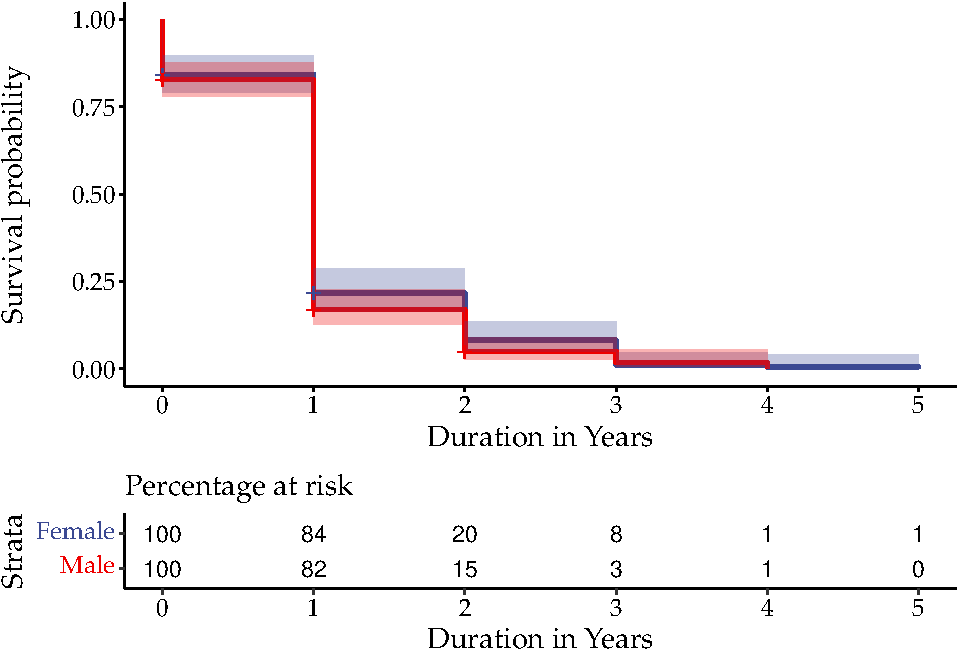
\includegraphics{figures/fig-survival-1} \caption{Survival analysis: duration of transition to first employment}\label{fig:fig-survival}
\end{figure}

\newpage

\hypertarget{survey-appendix-b}{%
\section*{Appendix B}\label{survey-appendix-b}}
\addcontentsline{toc}{section}{Appendix B}

\setcounter{table}{0}
\renewcommand{\thetable}{B\arabic{table}}

\providecommand{\docline}[3]{\noalign{\global\setlength{\arrayrulewidth}{#1}}\arrayrulecolor[HTML]{#2}\cline{#3}}

\setlength{\tabcolsep}{0pt}

\renewcommand*{\arraystretch}{1.25}

\begin{longtable}[c]{|p{0.75in}|p{0.75in}|p{0.75in}|p{0.75in}|p{0.75in}|p{0.75in}|p{0.75in}}

\caption{\textcolor[HTML]{000000}{\fontsize{11}{13}\selectfont{\global\setmainfont{Palatino}{Activity\ transition\ matrix:\ Combined\ data,\ 2013-2021}}}}\label{tab:tbl-fullmatrix}\\

\hhline{~~~~~~~}

\multicolumn{3}{!{\color[HTML]{000000}\vrule width 0pt}>{\raggedright}p{\dimexpr 2.25in+4\tabcolsep+2\arrayrulewidth}}{\textcolor[HTML]{000000}{\fontsize{8}{8}\selectfont{\global\setmainfont{Palatino}{}}}} & \multicolumn{4}{!{\color[HTML]{000000}\vrule width 0pt}>{\raggedright}p{\dimexpr 3in+6\tabcolsep+3\arrayrulewidth}!{\color[HTML]{000000}\vrule width 0pt}}{\textcolor[HTML]{000000}{\fontsize{8}{8}\selectfont{\global\setmainfont{Palatino}{To}}}} \\

\hhline{>{\arrayrulecolor[HTML]{666666}\global\arrayrulewidth=2pt}->{\arrayrulecolor[HTML]{666666}\global\arrayrulewidth=2pt}->{\arrayrulecolor[HTML]{666666}\global\arrayrulewidth=2pt}->{\arrayrulecolor[HTML]{666666}\global\arrayrulewidth=2pt}->{\arrayrulecolor[HTML]{666666}\global\arrayrulewidth=2pt}->{\arrayrulecolor[HTML]{666666}\global\arrayrulewidth=2pt}->{\arrayrulecolor[HTML]{666666}\global\arrayrulewidth=2pt}-}



\multicolumn{1}{!{\color[HTML]{000000}\vrule width 0pt}>{\raggedright}p{\dimexpr 0.75in+0\tabcolsep+0\arrayrulewidth}}{\textcolor[HTML]{000000}{\fontsize{8}{8}\selectfont{\global\setmainfont{Palatino}{From}}}} & \multicolumn{1}{!{\color[HTML]{000000}\vrule width 0pt}>{\raggedright}p{\dimexpr 0.75in+0\tabcolsep+0\arrayrulewidth}}{\textcolor[HTML]{000000}{\fontsize{8}{8}\selectfont{\global\setmainfont{Palatino}{In\ School}}}} & \multicolumn{1}{!{\color[HTML]{000000}\vrule width 0pt}>{\raggedright}p{\dimexpr 0.75in+0\tabcolsep+0\arrayrulewidth}}{\textcolor[HTML]{000000}{\fontsize{8}{8}\selectfont{\global\setmainfont{Palatino}{NEET}}}} & \multicolumn{1}{!{\color[HTML]{000000}\vrule width 0pt}>{\raggedright}p{\dimexpr 0.75in+0\tabcolsep+0\arrayrulewidth}}{\textcolor[HTML]{000000}{\fontsize{8}{8}\selectfont{\global\setmainfont{Palatino}{Self-Employed}}}} & \multicolumn{1}{!{\color[HTML]{000000}\vrule width 0pt}>{\raggedright}p{\dimexpr 0.75in+0\tabcolsep+0\arrayrulewidth}}{\textcolor[HTML]{000000}{\fontsize{8}{8}\selectfont{\global\setmainfont{Palatino}{Employed}}}} & \multicolumn{1}{!{\color[HTML]{000000}\vrule width 0pt}>{\raggedright}p{\dimexpr 0.75in+0\tabcolsep+0\arrayrulewidth}}{\textcolor[HTML]{000000}{\fontsize{8}{8}\selectfont{\global\setmainfont{Palatino}{Apprentice}}}} & \multicolumn{1}{!{\color[HTML]{000000}\vrule width 0pt}>{\raggedright}p{\dimexpr 0.75in+0\tabcolsep+0\arrayrulewidth}!{\color[HTML]{000000}\vrule width 0pt}}{\textcolor[HTML]{000000}{\fontsize{8}{8}\selectfont{\global\setmainfont{Palatino}{Total}}}} \\

\hhline{>{\arrayrulecolor[HTML]{666666}\global\arrayrulewidth=2pt}->{\arrayrulecolor[HTML]{666666}\global\arrayrulewidth=2pt}->{\arrayrulecolor[HTML]{666666}\global\arrayrulewidth=2pt}->{\arrayrulecolor[HTML]{666666}\global\arrayrulewidth=2pt}->{\arrayrulecolor[HTML]{666666}\global\arrayrulewidth=2pt}->{\arrayrulecolor[HTML]{666666}\global\arrayrulewidth=2pt}->{\arrayrulecolor[HTML]{666666}\global\arrayrulewidth=2pt}-}\endhead



\multicolumn{7}{!{\color[HTML]{FFFFFF}\vrule width 0pt}>{\raggedright}p{\dimexpr 5.25in+12\tabcolsep+6\arrayrulewidth}!{\color[HTML]{FFFFFF}\vrule width 0pt}}{\textcolor[HTML]{000000}{\fontsize{8}{8}\selectfont{\global\setmainfont{Palatino}{Row\ \%}}}\textcolor[HTML]{000000}{\fontsize{8}{8}\selectfont{\global\setmainfont{Palatino}{\linebreak }}}\textcolor[HTML]{000000}{\fontsize{8}{8}\selectfont{\global\setmainfont{Palatino}{(Column\ \%)}}}} \\

\endfoot



\multicolumn{1}{!{\color[HTML]{000000}\vrule width 0pt}>{\raggedright}p{\dimexpr 0.75in+0\tabcolsep+0\arrayrulewidth}}{\textcolor[HTML]{000000}{\fontsize{8}{8}\selectfont{\global\setmainfont{Palatino}{In\ School}}}} & \multicolumn{1}{!{\color[HTML]{000000}\vrule width 0pt}>{\raggedright}p{\dimexpr 0.75in+0\tabcolsep+0\arrayrulewidth}}{\textcolor[HTML]{000000}{\fontsize{8}{8}\selectfont{\global\setmainfont{Palatino}{84.51\%}}}\textcolor[HTML]{000000}{\fontsize{8}{8}\selectfont{\global\setmainfont{Palatino}{\linebreak }}}\textcolor[HTML]{000000}{\fontsize{8}{8}\selectfont{\global\setmainfont{Palatino}{(98.78\%)}}}} & \multicolumn{1}{!{\color[HTML]{000000}\vrule width 0pt}>{\raggedright}p{\dimexpr 0.75in+0\tabcolsep+0\arrayrulewidth}}{\textcolor[HTML]{000000}{\fontsize{8}{8}\selectfont{\global\setmainfont{Palatino}{4.07\%}}}\textcolor[HTML]{000000}{\fontsize{8}{8}\selectfont{\global\setmainfont{Palatino}{\linebreak }}}\textcolor[HTML]{000000}{\fontsize{8}{8}\selectfont{\global\setmainfont{Palatino}{(20.96\%)}}}} & \multicolumn{1}{!{\color[HTML]{000000}\vrule width 0pt}>{\raggedright}p{\dimexpr 0.75in+0\tabcolsep+0\arrayrulewidth}}{\textcolor[HTML]{000000}{\fontsize{8}{8}\selectfont{\global\setmainfont{Palatino}{2.83\%}}}\textcolor[HTML]{000000}{\fontsize{8}{8}\selectfont{\global\setmainfont{Palatino}{\linebreak }}}\textcolor[HTML]{000000}{\fontsize{8}{8}\selectfont{\global\setmainfont{Palatino}{(10.69\%)}}}} & \multicolumn{1}{!{\color[HTML]{000000}\vrule width 0pt}>{\raggedright}p{\dimexpr 0.75in+0\tabcolsep+0\arrayrulewidth}}{\textcolor[HTML]{000000}{\fontsize{8}{8}\selectfont{\global\setmainfont{Palatino}{5.57\%}}}\textcolor[HTML]{000000}{\fontsize{8}{8}\selectfont{\global\setmainfont{Palatino}{\linebreak }}}\textcolor[HTML]{000000}{\fontsize{8}{8}\selectfont{\global\setmainfont{Palatino}{(17.63\%)}}}} & \multicolumn{1}{!{\color[HTML]{000000}\vrule width 0pt}>{\raggedright}p{\dimexpr 0.75in+0\tabcolsep+0\arrayrulewidth}}{\textcolor[HTML]{000000}{\fontsize{8}{8}\selectfont{\global\setmainfont{Palatino}{3.02\%}}}\textcolor[HTML]{000000}{\fontsize{8}{8}\selectfont{\global\setmainfont{Palatino}{\linebreak }}}\textcolor[HTML]{000000}{\fontsize{8}{8}\selectfont{\global\setmainfont{Palatino}{(17.03\%)}}}} & \multicolumn{1}{!{\color[HTML]{000000}\vrule width 0pt}>{\raggedright}p{\dimexpr 0.75in+0\tabcolsep+0\arrayrulewidth}!{\color[HTML]{000000}\vrule width 0pt}}{\textcolor[HTML]{000000}{\fontsize{8}{8}\selectfont{\global\setmainfont{Palatino}{100.00\%}}}\textcolor[HTML]{000000}{\fontsize{8}{8}\selectfont{\global\setmainfont{Palatino}{\linebreak }}}\textcolor[HTML]{000000}{\fontsize{8}{8}\selectfont{\global\setmainfont{Palatino}{(165.08\%)}}}} \\





\multicolumn{1}{!{\color[HTML]{000000}\vrule width 0pt}>{\raggedright}p{\dimexpr 0.75in+0\tabcolsep+0\arrayrulewidth}}{\textcolor[HTML]{000000}{\fontsize{8}{8}\selectfont{\global\setmainfont{Palatino}{NEET}}}} & \multicolumn{1}{!{\color[HTML]{000000}\vrule width 0pt}>{\raggedright}p{\dimexpr 0.75in+0\tabcolsep+0\arrayrulewidth}}{\textcolor[HTML]{000000}{\fontsize{8}{8}\selectfont{\global\setmainfont{Palatino}{1.96\%}}}\textcolor[HTML]{000000}{\fontsize{8}{8}\selectfont{\global\setmainfont{Palatino}{\linebreak }}}\textcolor[HTML]{000000}{\fontsize{8}{8}\selectfont{\global\setmainfont{Palatino}{(0.41\%)}}}} & \multicolumn{1}{!{\color[HTML]{000000}\vrule width 0pt}>{\raggedright}p{\dimexpr 0.75in+0\tabcolsep+0\arrayrulewidth}}{\textcolor[HTML]{000000}{\fontsize{8}{8}\selectfont{\global\setmainfont{Palatino}{62.53\%}}}\textcolor[HTML]{000000}{\fontsize{8}{8}\selectfont{\global\setmainfont{Palatino}{\linebreak }}}\textcolor[HTML]{000000}{\fontsize{8}{8}\selectfont{\global\setmainfont{Palatino}{(57.29\%)}}}} & \multicolumn{1}{!{\color[HTML]{000000}\vrule width 0pt}>{\raggedright}p{\dimexpr 0.75in+0\tabcolsep+0\arrayrulewidth}}{\textcolor[HTML]{000000}{\fontsize{8}{8}\selectfont{\global\setmainfont{Palatino}{11.11\%}}}\textcolor[HTML]{000000}{\fontsize{8}{8}\selectfont{\global\setmainfont{Palatino}{\linebreak }}}\textcolor[HTML]{000000}{\fontsize{8}{8}\selectfont{\global\setmainfont{Palatino}{(7.47\%)}}}} & \multicolumn{1}{!{\color[HTML]{000000}\vrule width 0pt}>{\raggedright}p{\dimexpr 0.75in+0\tabcolsep+0\arrayrulewidth}}{\textcolor[HTML]{000000}{\fontsize{8}{8}\selectfont{\global\setmainfont{Palatino}{16.56\%}}}\textcolor[HTML]{000000}{\fontsize{8}{8}\selectfont{\global\setmainfont{Palatino}{\linebreak }}}\textcolor[HTML]{000000}{\fontsize{8}{8}\selectfont{\global\setmainfont{Palatino}{(9.30\%)}}}} & \multicolumn{1}{!{\color[HTML]{000000}\vrule width 0pt}>{\raggedright}p{\dimexpr 0.75in+0\tabcolsep+0\arrayrulewidth}}{\textcolor[HTML]{000000}{\fontsize{8}{8}\selectfont{\global\setmainfont{Palatino}{7.84\%}}}\textcolor[HTML]{000000}{\fontsize{8}{8}\selectfont{\global\setmainfont{Palatino}{\linebreak }}}\textcolor[HTML]{000000}{\fontsize{8}{8}\selectfont{\global\setmainfont{Palatino}{(7.86\%)}}}} & \multicolumn{1}{!{\color[HTML]{000000}\vrule width 0pt}>{\raggedright}p{\dimexpr 0.75in+0\tabcolsep+0\arrayrulewidth}!{\color[HTML]{000000}\vrule width 0pt}}{\textcolor[HTML]{000000}{\fontsize{8}{8}\selectfont{\global\setmainfont{Palatino}{100.00\%}}}\textcolor[HTML]{000000}{\fontsize{8}{8}\selectfont{\global\setmainfont{Palatino}{\linebreak }}}\textcolor[HTML]{000000}{\fontsize{8}{8}\selectfont{\global\setmainfont{Palatino}{(82.32\%)}}}} \\





\multicolumn{1}{!{\color[HTML]{000000}\vrule width 0pt}>{\raggedright}p{\dimexpr 0.75in+0\tabcolsep+0\arrayrulewidth}}{\textcolor[HTML]{000000}{\fontsize{8}{8}\selectfont{\global\setmainfont{Palatino}{Self-Employed}}}} & \multicolumn{1}{!{\color[HTML]{000000}\vrule width 0pt}>{\raggedright}p{\dimexpr 0.75in+0\tabcolsep+0\arrayrulewidth}}{\textcolor[HTML]{000000}{\fontsize{8}{8}\selectfont{\global\setmainfont{Palatino}{1.62\%}}}\textcolor[HTML]{000000}{\fontsize{8}{8}\selectfont{\global\setmainfont{Palatino}{\linebreak }}}\textcolor[HTML]{000000}{\fontsize{8}{8}\selectfont{\global\setmainfont{Palatino}{(0.41\%)}}}} & \multicolumn{1}{!{\color[HTML]{000000}\vrule width 0pt}>{\raggedright}p{\dimexpr 0.75in+0\tabcolsep+0\arrayrulewidth}}{\textcolor[HTML]{000000}{\fontsize{8}{8}\selectfont{\global\setmainfont{Palatino}{5.57\%}}}\textcolor[HTML]{000000}{\fontsize{8}{8}\selectfont{\global\setmainfont{Palatino}{\linebreak }}}\textcolor[HTML]{000000}{\fontsize{8}{8}\selectfont{\global\setmainfont{Palatino}{(6.19\%)}}}} & \multicolumn{1}{!{\color[HTML]{000000}\vrule width 0pt}>{\raggedright}p{\dimexpr 0.75in+0\tabcolsep+0\arrayrulewidth}}{\textcolor[HTML]{000000}{\fontsize{8}{8}\selectfont{\global\setmainfont{Palatino}{87.07\%}}}\textcolor[HTML]{000000}{\fontsize{8}{8}\selectfont{\global\setmainfont{Palatino}{\linebreak }}}\textcolor[HTML]{000000}{\fontsize{8}{8}\selectfont{\global\setmainfont{Palatino}{(71.01\%)}}}} & \multicolumn{1}{!{\color[HTML]{000000}\vrule width 0pt}>{\raggedright}p{\dimexpr 0.75in+0\tabcolsep+0\arrayrulewidth}}{\textcolor[HTML]{000000}{\fontsize{8}{8}\selectfont{\global\setmainfont{Palatino}{3.95\%}}}\textcolor[HTML]{000000}{\fontsize{8}{8}\selectfont{\global\setmainfont{Palatino}{\linebreak }}}\textcolor[HTML]{000000}{\fontsize{8}{8}\selectfont{\global\setmainfont{Palatino}{(2.69\%)}}}} & \multicolumn{1}{!{\color[HTML]{000000}\vrule width 0pt}>{\raggedright}p{\dimexpr 0.75in+0\tabcolsep+0\arrayrulewidth}}{\textcolor[HTML]{000000}{\fontsize{8}{8}\selectfont{\global\setmainfont{Palatino}{1.80\%}}}\textcolor[HTML]{000000}{\fontsize{8}{8}\selectfont{\global\setmainfont{Palatino}{\linebreak }}}\textcolor[HTML]{000000}{\fontsize{8}{8}\selectfont{\global\setmainfont{Palatino}{(2.18\%)}}}} & \multicolumn{1}{!{\color[HTML]{000000}\vrule width 0pt}>{\raggedright}p{\dimexpr 0.75in+0\tabcolsep+0\arrayrulewidth}!{\color[HTML]{000000}\vrule width 0pt}}{\textcolor[HTML]{000000}{\fontsize{8}{8}\selectfont{\global\setmainfont{Palatino}{100.00\%}}}\textcolor[HTML]{000000}{\fontsize{8}{8}\selectfont{\global\setmainfont{Palatino}{\linebreak }}}\textcolor[HTML]{000000}{\fontsize{8}{8}\selectfont{\global\setmainfont{Palatino}{(82.48\%)}}}} \\





\multicolumn{1}{!{\color[HTML]{000000}\vrule width 0pt}>{\raggedright}p{\dimexpr 0.75in+0\tabcolsep+0\arrayrulewidth}}{\textcolor[HTML]{000000}{\fontsize{8}{8}\selectfont{\global\setmainfont{Palatino}{Employed}}}} & \multicolumn{1}{!{\color[HTML]{000000}\vrule width 0pt}>{\raggedright}p{\dimexpr 0.75in+0\tabcolsep+0\arrayrulewidth}}{\textcolor[HTML]{000000}{\fontsize{8}{8}\selectfont{\global\setmainfont{Palatino}{1.30\%}}}\textcolor[HTML]{000000}{\fontsize{8}{8}\selectfont{\global\setmainfont{Palatino}{\linebreak }}}\textcolor[HTML]{000000}{\fontsize{8}{8}\selectfont{\global\setmainfont{Palatino}{(0.36\%)}}}} & \multicolumn{1}{!{\color[HTML]{000000}\vrule width 0pt}>{\raggedright}p{\dimexpr 0.75in+0\tabcolsep+0\arrayrulewidth}}{\textcolor[HTML]{000000}{\fontsize{8}{8}\selectfont{\global\setmainfont{Palatino}{8.10\%}}}\textcolor[HTML]{000000}{\fontsize{8}{8}\selectfont{\global\setmainfont{Palatino}{\linebreak }}}\textcolor[HTML]{000000}{\fontsize{8}{8}\selectfont{\global\setmainfont{Palatino}{(9.98\%)}}}} & \multicolumn{1}{!{\color[HTML]{000000}\vrule width 0pt}>{\raggedright}p{\dimexpr 0.75in+0\tabcolsep+0\arrayrulewidth}}{\textcolor[HTML]{000000}{\fontsize{8}{8}\selectfont{\global\setmainfont{Palatino}{4.70\%}}}\textcolor[HTML]{000000}{\fontsize{8}{8}\selectfont{\global\setmainfont{Palatino}{\linebreak }}}\textcolor[HTML]{000000}{\fontsize{8}{8}\selectfont{\global\setmainfont{Palatino}{(4.25\%)}}}} & \multicolumn{1}{!{\color[HTML]{000000}\vrule width 0pt}>{\raggedright}p{\dimexpr 0.75in+0\tabcolsep+0\arrayrulewidth}}{\textcolor[HTML]{000000}{\fontsize{8}{8}\selectfont{\global\setmainfont{Palatino}{83.95\%}}}\textcolor[HTML]{000000}{\fontsize{8}{8}\selectfont{\global\setmainfont{Palatino}{\linebreak }}}\textcolor[HTML]{000000}{\fontsize{8}{8}\selectfont{\global\setmainfont{Palatino}{(63.40\%)}}}} & \multicolumn{1}{!{\color[HTML]{000000}\vrule width 0pt}>{\raggedright}p{\dimexpr 0.75in+0\tabcolsep+0\arrayrulewidth}}{\textcolor[HTML]{000000}{\fontsize{8}{8}\selectfont{\global\setmainfont{Palatino}{1.94\%}}}\textcolor[HTML]{000000}{\fontsize{8}{8}\selectfont{\global\setmainfont{Palatino}{\linebreak }}}\textcolor[HTML]{000000}{\fontsize{8}{8}\selectfont{\global\setmainfont{Palatino}{(2.62\%)}}}} & \multicolumn{1}{!{\color[HTML]{000000}\vrule width 0pt}>{\raggedright}p{\dimexpr 0.75in+0\tabcolsep+0\arrayrulewidth}!{\color[HTML]{000000}\vrule width 0pt}}{\textcolor[HTML]{000000}{\fontsize{8}{8}\selectfont{\global\setmainfont{Palatino}{100.00\%}}}\textcolor[HTML]{000000}{\fontsize{8}{8}\selectfont{\global\setmainfont{Palatino}{\linebreak }}}\textcolor[HTML]{000000}{\fontsize{8}{8}\selectfont{\global\setmainfont{Palatino}{(80.61\%)}}}} \\





\multicolumn{1}{!{\color[HTML]{000000}\vrule width 0pt}>{\raggedright}p{\dimexpr 0.75in+0\tabcolsep+0\arrayrulewidth}}{\textcolor[HTML]{000000}{\fontsize{8}{8}\selectfont{\global\setmainfont{Palatino}{Apprentice}}}} & \multicolumn{1}{!{\color[HTML]{000000}\vrule width 0pt}>{\raggedright}p{\dimexpr 0.75in+0\tabcolsep+0\arrayrulewidth}}{\textcolor[HTML]{000000}{\fontsize{8}{8}\selectfont{\global\setmainfont{Palatino}{0.22\%}}}\textcolor[HTML]{000000}{\fontsize{8}{8}\selectfont{\global\setmainfont{Palatino}{\linebreak }}}\textcolor[HTML]{000000}{\fontsize{8}{8}\selectfont{\global\setmainfont{Palatino}{(0.05\%)}}}} & \multicolumn{1}{!{\color[HTML]{000000}\vrule width 0pt}>{\raggedright}p{\dimexpr 0.75in+0\tabcolsep+0\arrayrulewidth}}{\textcolor[HTML]{000000}{\fontsize{8}{8}\selectfont{\global\setmainfont{Palatino}{6.18\%}}}\textcolor[HTML]{000000}{\fontsize{8}{8}\selectfont{\global\setmainfont{Palatino}{\linebreak }}}\textcolor[HTML]{000000}{\fontsize{8}{8}\selectfont{\global\setmainfont{Palatino}{(5.59\%)}}}} & \multicolumn{1}{!{\color[HTML]{000000}\vrule width 0pt}>{\raggedright}p{\dimexpr 0.75in+0\tabcolsep+0\arrayrulewidth}}{\textcolor[HTML]{000000}{\fontsize{8}{8}\selectfont{\global\setmainfont{Palatino}{9.93\%}}}\textcolor[HTML]{000000}{\fontsize{8}{8}\selectfont{\global\setmainfont{Palatino}{\linebreak }}}\textcolor[HTML]{000000}{\fontsize{8}{8}\selectfont{\global\setmainfont{Palatino}{(6.59\%)}}}} & \multicolumn{1}{!{\color[HTML]{000000}\vrule width 0pt}>{\raggedright}p{\dimexpr 0.75in+0\tabcolsep+0\arrayrulewidth}}{\textcolor[HTML]{000000}{\fontsize{8}{8}\selectfont{\global\setmainfont{Palatino}{12.58\%}}}\textcolor[HTML]{000000}{\fontsize{8}{8}\selectfont{\global\setmainfont{Palatino}{\linebreak }}}\textcolor[HTML]{000000}{\fontsize{8}{8}\selectfont{\global\setmainfont{Palatino}{(6.98\%)}}}} & \multicolumn{1}{!{\color[HTML]{000000}\vrule width 0pt}>{\raggedright}p{\dimexpr 0.75in+0\tabcolsep+0\arrayrulewidth}}{\textcolor[HTML]{000000}{\fontsize{8}{8}\selectfont{\global\setmainfont{Palatino}{71.08\%}}}\textcolor[HTML]{000000}{\fontsize{8}{8}\selectfont{\global\setmainfont{Palatino}{\linebreak }}}\textcolor[HTML]{000000}{\fontsize{8}{8}\selectfont{\global\setmainfont{Palatino}{(70.31\%)}}}} & \multicolumn{1}{!{\color[HTML]{000000}\vrule width 0pt}>{\raggedright}p{\dimexpr 0.75in+0\tabcolsep+0\arrayrulewidth}!{\color[HTML]{000000}\vrule width 0pt}}{\textcolor[HTML]{000000}{\fontsize{8}{8}\selectfont{\global\setmainfont{Palatino}{100.00\%}}}\textcolor[HTML]{000000}{\fontsize{8}{8}\selectfont{\global\setmainfont{Palatino}{\linebreak }}}\textcolor[HTML]{000000}{\fontsize{8}{8}\selectfont{\global\setmainfont{Palatino}{(89.51\%)}}}} \\





\multicolumn{1}{!{\color[HTML]{000000}\vrule width 0pt}>{\raggedright}p{\dimexpr 0.75in+0\tabcolsep+0\arrayrulewidth}}{\textcolor[HTML]{000000}{\fontsize{8}{8}\selectfont{\global\setmainfont{Palatino}{Total}}}} & \multicolumn{1}{!{\color[HTML]{000000}\vrule width 0pt}>{\raggedright}p{\dimexpr 0.75in+0\tabcolsep+0\arrayrulewidth}}{\textcolor[HTML]{000000}{\fontsize{8}{8}\selectfont{\global\setmainfont{Palatino}{89.61\%}}}\textcolor[HTML]{000000}{\fontsize{8}{8}\selectfont{\global\setmainfont{Palatino}{\linebreak }}}\textcolor[HTML]{000000}{\fontsize{8}{8}\selectfont{\global\setmainfont{Palatino}{(100.00\%)}}}} & \multicolumn{1}{!{\color[HTML]{000000}\vrule width 0pt}>{\raggedright}p{\dimexpr 0.75in+0\tabcolsep+0\arrayrulewidth}}{\textcolor[HTML]{000000}{\fontsize{8}{8}\selectfont{\global\setmainfont{Palatino}{86.44\%}}}\textcolor[HTML]{000000}{\fontsize{8}{8}\selectfont{\global\setmainfont{Palatino}{\linebreak }}}\textcolor[HTML]{000000}{\fontsize{8}{8}\selectfont{\global\setmainfont{Palatino}{(100.00\%)}}}} & \multicolumn{1}{!{\color[HTML]{000000}\vrule width 0pt}>{\raggedright}p{\dimexpr 0.75in+0\tabcolsep+0\arrayrulewidth}}{\textcolor[HTML]{000000}{\fontsize{8}{8}\selectfont{\global\setmainfont{Palatino}{115.64\%}}}\textcolor[HTML]{000000}{\fontsize{8}{8}\selectfont{\global\setmainfont{Palatino}{\linebreak }}}\textcolor[HTML]{000000}{\fontsize{8}{8}\selectfont{\global\setmainfont{Palatino}{(100.00\%)}}}} & \multicolumn{1}{!{\color[HTML]{000000}\vrule width 0pt}>{\raggedright}p{\dimexpr 0.75in+0\tabcolsep+0\arrayrulewidth}}{\textcolor[HTML]{000000}{\fontsize{8}{8}\selectfont{\global\setmainfont{Palatino}{122.62\%}}}\textcolor[HTML]{000000}{\fontsize{8}{8}\selectfont{\global\setmainfont{Palatino}{\linebreak }}}\textcolor[HTML]{000000}{\fontsize{8}{8}\selectfont{\global\setmainfont{Palatino}{(100.00\%)}}}} & \multicolumn{1}{!{\color[HTML]{000000}\vrule width 0pt}>{\raggedright}p{\dimexpr 0.75in+0\tabcolsep+0\arrayrulewidth}}{\textcolor[HTML]{000000}{\fontsize{8}{8}\selectfont{\global\setmainfont{Palatino}{85.68\%}}}\textcolor[HTML]{000000}{\fontsize{8}{8}\selectfont{\global\setmainfont{Palatino}{\linebreak }}}\textcolor[HTML]{000000}{\fontsize{8}{8}\selectfont{\global\setmainfont{Palatino}{(100.00\%)}}}} & \multicolumn{1}{!{\color[HTML]{000000}\vrule width 0pt}>{\raggedright}p{\dimexpr 0.75in+0\tabcolsep+0\arrayrulewidth}!{\color[HTML]{000000}\vrule width 0pt}}{\textcolor[HTML]{000000}{\fontsize{8}{8}\selectfont{\global\setmainfont{Palatino}{}}}} \\

\hhline{>{\arrayrulecolor[HTML]{666666}\global\arrayrulewidth=2pt}->{\arrayrulecolor[HTML]{666666}\global\arrayrulewidth=2pt}->{\arrayrulecolor[HTML]{666666}\global\arrayrulewidth=2pt}->{\arrayrulecolor[HTML]{666666}\global\arrayrulewidth=2pt}->{\arrayrulecolor[HTML]{666666}\global\arrayrulewidth=2pt}->{\arrayrulecolor[HTML]{666666}\global\arrayrulewidth=2pt}->{\arrayrulecolor[HTML]{666666}\global\arrayrulewidth=2pt}-}



\end{longtable}

\providecommand{\docline}[3]{\noalign{\global\setlength{\arrayrulewidth}{#1}}\arrayrulecolor[HTML]{#2}\cline{#3}}

\setlength{\tabcolsep}{0pt}

\renewcommand*{\arraystretch}{1.25}

\begin{longtable}[c]{|p{0.75in}|p{0.75in}|p{0.75in}|p{0.75in}|p{0.75in}|p{0.75in}|p{0.75in}}

\caption{\textcolor[HTML]{000000}{\fontsize{11}{13}\selectfont{\global\setmainfont{Palatino}{Activity\ transition\ matrix:\ Event\ History,\ 2013-2019}}}}\label{tab:tbl-historymatrix}\\

\hhline{~~~~~~~}

\multicolumn{3}{!{\color[HTML]{000000}\vrule width 0pt}>{\raggedright}p{\dimexpr 2.25in+4\tabcolsep+2\arrayrulewidth}}{\textcolor[HTML]{000000}{\fontsize{9}{9}\selectfont{\global\setmainfont{Palatino}{}}}} & \multicolumn{4}{!{\color[HTML]{000000}\vrule width 0pt}>{\raggedright}p{\dimexpr 3in+6\tabcolsep+3\arrayrulewidth}!{\color[HTML]{000000}\vrule width 0pt}}{\textcolor[HTML]{000000}{\fontsize{9}{9}\selectfont{\global\setmainfont{Palatino}{To}}}} \\

\hhline{>{\arrayrulecolor[HTML]{666666}\global\arrayrulewidth=2pt}->{\arrayrulecolor[HTML]{666666}\global\arrayrulewidth=2pt}->{\arrayrulecolor[HTML]{666666}\global\arrayrulewidth=2pt}->{\arrayrulecolor[HTML]{666666}\global\arrayrulewidth=2pt}->{\arrayrulecolor[HTML]{666666}\global\arrayrulewidth=2pt}->{\arrayrulecolor[HTML]{666666}\global\arrayrulewidth=2pt}->{\arrayrulecolor[HTML]{666666}\global\arrayrulewidth=2pt}-}



\multicolumn{1}{!{\color[HTML]{000000}\vrule width 0pt}>{\raggedright}p{\dimexpr 0.75in+0\tabcolsep+0\arrayrulewidth}}{\textcolor[HTML]{000000}{\fontsize{9}{9}\selectfont{\global\setmainfont{Palatino}{From}}}} & \multicolumn{1}{!{\color[HTML]{000000}\vrule width 0pt}>{\raggedright}p{\dimexpr 0.75in+0\tabcolsep+0\arrayrulewidth}}{\textcolor[HTML]{000000}{\fontsize{9}{9}\selectfont{\global\setmainfont{Palatino}{In\ School}}}} & \multicolumn{1}{!{\color[HTML]{000000}\vrule width 0pt}>{\raggedright}p{\dimexpr 0.75in+0\tabcolsep+0\arrayrulewidth}}{\textcolor[HTML]{000000}{\fontsize{9}{9}\selectfont{\global\setmainfont{Palatino}{NEET}}}} & \multicolumn{1}{!{\color[HTML]{000000}\vrule width 0pt}>{\raggedright}p{\dimexpr 0.75in+0\tabcolsep+0\arrayrulewidth}}{\textcolor[HTML]{000000}{\fontsize{9}{9}\selectfont{\global\setmainfont{Palatino}{Self-Employed}}}} & \multicolumn{1}{!{\color[HTML]{000000}\vrule width 0pt}>{\raggedright}p{\dimexpr 0.75in+0\tabcolsep+0\arrayrulewidth}}{\textcolor[HTML]{000000}{\fontsize{9}{9}\selectfont{\global\setmainfont{Palatino}{Employed}}}} & \multicolumn{1}{!{\color[HTML]{000000}\vrule width 0pt}>{\raggedright}p{\dimexpr 0.75in+0\tabcolsep+0\arrayrulewidth}}{\textcolor[HTML]{000000}{\fontsize{9}{9}\selectfont{\global\setmainfont{Palatino}{Apprentice}}}} & \multicolumn{1}{!{\color[HTML]{000000}\vrule width 0pt}>{\raggedright}p{\dimexpr 0.75in+0\tabcolsep+0\arrayrulewidth}!{\color[HTML]{000000}\vrule width 0pt}}{\textcolor[HTML]{000000}{\fontsize{9}{9}\selectfont{\global\setmainfont{Palatino}{Total}}}} \\

\hhline{>{\arrayrulecolor[HTML]{666666}\global\arrayrulewidth=2pt}->{\arrayrulecolor[HTML]{666666}\global\arrayrulewidth=2pt}->{\arrayrulecolor[HTML]{666666}\global\arrayrulewidth=2pt}->{\arrayrulecolor[HTML]{666666}\global\arrayrulewidth=2pt}->{\arrayrulecolor[HTML]{666666}\global\arrayrulewidth=2pt}->{\arrayrulecolor[HTML]{666666}\global\arrayrulewidth=2pt}->{\arrayrulecolor[HTML]{666666}\global\arrayrulewidth=2pt}-}\endhead



\multicolumn{7}{!{\color[HTML]{FFFFFF}\vrule width 0pt}>{\raggedright}p{\dimexpr 5.25in+12\tabcolsep+6\arrayrulewidth}!{\color[HTML]{FFFFFF}\vrule width 0pt}}{\textcolor[HTML]{000000}{\fontsize{9}{9}\selectfont{\global\setmainfont{Palatino}{Row\ \%}}}\textcolor[HTML]{000000}{\fontsize{9}{9}\selectfont{\global\setmainfont{Palatino}{\linebreak }}}\textcolor[HTML]{000000}{\fontsize{9}{9}\selectfont{\global\setmainfont{Palatino}{(Column\ \%)}}}} \\

\endfoot



\multicolumn{1}{!{\color[HTML]{000000}\vrule width 0pt}>{\raggedright}p{\dimexpr 0.75in+0\tabcolsep+0\arrayrulewidth}}{\textcolor[HTML]{000000}{\fontsize{9}{9}\selectfont{\global\setmainfont{Palatino}{In\ School}}}} & \multicolumn{1}{!{\color[HTML]{000000}\vrule width 0pt}>{\raggedright}p{\dimexpr 0.75in+0\tabcolsep+0\arrayrulewidth}}{\textcolor[HTML]{000000}{\fontsize{9}{9}\selectfont{\global\setmainfont{Palatino}{85.68\%}}}\textcolor[HTML]{000000}{\fontsize{9}{9}\selectfont{\global\setmainfont{Palatino}{\linebreak }}}\textcolor[HTML]{000000}{\fontsize{9}{9}\selectfont{\global\setmainfont{Palatino}{(98.91\%)}}}} & \multicolumn{1}{!{\color[HTML]{000000}\vrule width 0pt}>{\raggedright}p{\dimexpr 0.75in+0\tabcolsep+0\arrayrulewidth}}{\textcolor[HTML]{000000}{\fontsize{9}{9}\selectfont{\global\setmainfont{Palatino}{3.85\%}}}\textcolor[HTML]{000000}{\fontsize{9}{9}\selectfont{\global\setmainfont{Palatino}{\linebreak }}}\textcolor[HTML]{000000}{\fontsize{9}{9}\selectfont{\global\setmainfont{Palatino}{(21.74\%)}}}} & \multicolumn{1}{!{\color[HTML]{000000}\vrule width 0pt}>{\raggedright}p{\dimexpr 0.75in+0\tabcolsep+0\arrayrulewidth}}{\textcolor[HTML]{000000}{\fontsize{9}{9}\selectfont{\global\setmainfont{Palatino}{2.61\%}}}\textcolor[HTML]{000000}{\fontsize{9}{9}\selectfont{\global\setmainfont{Palatino}{\linebreak }}}\textcolor[HTML]{000000}{\fontsize{9}{9}\selectfont{\global\setmainfont{Palatino}{(11.36\%)}}}} & \multicolumn{1}{!{\color[HTML]{000000}\vrule width 0pt}>{\raggedright}p{\dimexpr 0.75in+0\tabcolsep+0\arrayrulewidth}}{\textcolor[HTML]{000000}{\fontsize{9}{9}\selectfont{\global\setmainfont{Palatino}{4.92\%}}}\textcolor[HTML]{000000}{\fontsize{9}{9}\selectfont{\global\setmainfont{Palatino}{\linebreak }}}\textcolor[HTML]{000000}{\fontsize{9}{9}\selectfont{\global\setmainfont{Palatino}{(18.40\%)}}}} & \multicolumn{1}{!{\color[HTML]{000000}\vrule width 0pt}>{\raggedright}p{\dimexpr 0.75in+0\tabcolsep+0\arrayrulewidth}}{\textcolor[HTML]{000000}{\fontsize{9}{9}\selectfont{\global\setmainfont{Palatino}{2.95\%}}}\textcolor[HTML]{000000}{\fontsize{9}{9}\selectfont{\global\setmainfont{Palatino}{\linebreak }}}\textcolor[HTML]{000000}{\fontsize{9}{9}\selectfont{\global\setmainfont{Palatino}{(17.25\%)}}}} & \multicolumn{1}{!{\color[HTML]{000000}\vrule width 0pt}>{\raggedright}p{\dimexpr 0.75in+0\tabcolsep+0\arrayrulewidth}!{\color[HTML]{000000}\vrule width 0pt}}{\textcolor[HTML]{000000}{\fontsize{9}{9}\selectfont{\global\setmainfont{Palatino}{100.00\%}}}\textcolor[HTML]{000000}{\fontsize{9}{9}\selectfont{\global\setmainfont{Palatino}{\linebreak }}}\textcolor[HTML]{000000}{\fontsize{9}{9}\selectfont{\global\setmainfont{Palatino}{(167.66\%)}}}} \\





\multicolumn{1}{!{\color[HTML]{000000}\vrule width 0pt}>{\raggedright}p{\dimexpr 0.75in+0\tabcolsep+0\arrayrulewidth}}{\textcolor[HTML]{000000}{\fontsize{9}{9}\selectfont{\global\setmainfont{Palatino}{NEET}}}} & \multicolumn{1}{!{\color[HTML]{000000}\vrule width 0pt}>{\raggedright}p{\dimexpr 0.75in+0\tabcolsep+0\arrayrulewidth}}{\textcolor[HTML]{000000}{\fontsize{9}{9}\selectfont{\global\setmainfont{Palatino}{1.82\%}}}\textcolor[HTML]{000000}{\fontsize{9}{9}\selectfont{\global\setmainfont{Palatino}{\linebreak }}}\textcolor[HTML]{000000}{\fontsize{9}{9}\selectfont{\global\setmainfont{Palatino}{(0.35\%)}}}} & \multicolumn{1}{!{\color[HTML]{000000}\vrule width 0pt}>{\raggedright}p{\dimexpr 0.75in+0\tabcolsep+0\arrayrulewidth}}{\textcolor[HTML]{000000}{\fontsize{9}{9}\selectfont{\global\setmainfont{Palatino}{64.94\%}}}\textcolor[HTML]{000000}{\fontsize{9}{9}\selectfont{\global\setmainfont{Palatino}{\linebreak }}}\textcolor[HTML]{000000}{\fontsize{9}{9}\selectfont{\global\setmainfont{Palatino}{(60.39\%)}}}} & \multicolumn{1}{!{\color[HTML]{000000}\vrule width 0pt}>{\raggedright}p{\dimexpr 0.75in+0\tabcolsep+0\arrayrulewidth}}{\textcolor[HTML]{000000}{\fontsize{9}{9}\selectfont{\global\setmainfont{Palatino}{11.17\%}}}\textcolor[HTML]{000000}{\fontsize{9}{9}\selectfont{\global\setmainfont{Palatino}{\linebreak }}}\textcolor[HTML]{000000}{\fontsize{9}{9}\selectfont{\global\setmainfont{Palatino}{(8.01\%)}}}} & \multicolumn{1}{!{\color[HTML]{000000}\vrule width 0pt}>{\raggedright}p{\dimexpr 0.75in+0\tabcolsep+0\arrayrulewidth}}{\textcolor[HTML]{000000}{\fontsize{9}{9}\selectfont{\global\setmainfont{Palatino}{14.29\%}}}\textcolor[HTML]{000000}{\fontsize{9}{9}\selectfont{\global\setmainfont{Palatino}{\linebreak }}}\textcolor[HTML]{000000}{\fontsize{9}{9}\selectfont{\global\setmainfont{Palatino}{(8.80\%)}}}} & \multicolumn{1}{!{\color[HTML]{000000}\vrule width 0pt}>{\raggedright}p{\dimexpr 0.75in+0\tabcolsep+0\arrayrulewidth}}{\textcolor[HTML]{000000}{\fontsize{9}{9}\selectfont{\global\setmainfont{Palatino}{7.79\%}}}\textcolor[HTML]{000000}{\fontsize{9}{9}\selectfont{\global\setmainfont{Palatino}{\linebreak }}}\textcolor[HTML]{000000}{\fontsize{9}{9}\selectfont{\global\setmainfont{Palatino}{(7.50\%)}}}} & \multicolumn{1}{!{\color[HTML]{000000}\vrule width 0pt}>{\raggedright}p{\dimexpr 0.75in+0\tabcolsep+0\arrayrulewidth}!{\color[HTML]{000000}\vrule width 0pt}}{\textcolor[HTML]{000000}{\fontsize{9}{9}\selectfont{\global\setmainfont{Palatino}{100.00\%}}}\textcolor[HTML]{000000}{\fontsize{9}{9}\selectfont{\global\setmainfont{Palatino}{\linebreak }}}\textcolor[HTML]{000000}{\fontsize{9}{9}\selectfont{\global\setmainfont{Palatino}{(85.04\%)}}}} \\





\multicolumn{1}{!{\color[HTML]{000000}\vrule width 0pt}>{\raggedright}p{\dimexpr 0.75in+0\tabcolsep+0\arrayrulewidth}}{\textcolor[HTML]{000000}{\fontsize{9}{9}\selectfont{\global\setmainfont{Palatino}{Self-Employed}}}} & \multicolumn{1}{!{\color[HTML]{000000}\vrule width 0pt}>{\raggedright}p{\dimexpr 0.75in+0\tabcolsep+0\arrayrulewidth}}{\textcolor[HTML]{000000}{\fontsize{9}{9}\selectfont{\global\setmainfont{Palatino}{1.87\%}}}\textcolor[HTML]{000000}{\fontsize{9}{9}\selectfont{\global\setmainfont{Palatino}{\linebreak }}}\textcolor[HTML]{000000}{\fontsize{9}{9}\selectfont{\global\setmainfont{Palatino}{(0.39\%)}}}} & \multicolumn{1}{!{\color[HTML]{000000}\vrule width 0pt}>{\raggedright}p{\dimexpr 0.75in+0\tabcolsep+0\arrayrulewidth}}{\textcolor[HTML]{000000}{\fontsize{9}{9}\selectfont{\global\setmainfont{Palatino}{4.68\%}}}\textcolor[HTML]{000000}{\fontsize{9}{9}\selectfont{\global\setmainfont{Palatino}{\linebreak }}}\textcolor[HTML]{000000}{\fontsize{9}{9}\selectfont{\global\setmainfont{Palatino}{(4.83\%)}}}} & \multicolumn{1}{!{\color[HTML]{000000}\vrule width 0pt}>{\raggedright}p{\dimexpr 0.75in+0\tabcolsep+0\arrayrulewidth}}{\textcolor[HTML]{000000}{\fontsize{9}{9}\selectfont{\global\setmainfont{Palatino}{87.82\%}}}\textcolor[HTML]{000000}{\fontsize{9}{9}\selectfont{\global\setmainfont{Palatino}{\linebreak }}}\textcolor[HTML]{000000}{\fontsize{9}{9}\selectfont{\global\setmainfont{Palatino}{(69.83\%)}}}} & \multicolumn{1}{!{\color[HTML]{000000}\vrule width 0pt}>{\raggedright}p{\dimexpr 0.75in+0\tabcolsep+0\arrayrulewidth}}{\textcolor[HTML]{000000}{\fontsize{9}{9}\selectfont{\global\setmainfont{Palatino}{3.75\%}}}\textcolor[HTML]{000000}{\fontsize{9}{9}\selectfont{\global\setmainfont{Palatino}{\linebreak }}}\textcolor[HTML]{000000}{\fontsize{9}{9}\selectfont{\global\setmainfont{Palatino}{(2.56\%)}}}} & \multicolumn{1}{!{\color[HTML]{000000}\vrule width 0pt}>{\raggedright}p{\dimexpr 0.75in+0\tabcolsep+0\arrayrulewidth}}{\textcolor[HTML]{000000}{\fontsize{9}{9}\selectfont{\global\setmainfont{Palatino}{1.87\%}}}\textcolor[HTML]{000000}{\fontsize{9}{9}\selectfont{\global\setmainfont{Palatino}{\linebreak }}}\textcolor[HTML]{000000}{\fontsize{9}{9}\selectfont{\global\setmainfont{Palatino}{(2.00\%)}}}} & \multicolumn{1}{!{\color[HTML]{000000}\vrule width 0pt}>{\raggedright}p{\dimexpr 0.75in+0\tabcolsep+0\arrayrulewidth}!{\color[HTML]{000000}\vrule width 0pt}}{\textcolor[HTML]{000000}{\fontsize{9}{9}\selectfont{\global\setmainfont{Palatino}{100.00\%}}}\textcolor[HTML]{000000}{\fontsize{9}{9}\selectfont{\global\setmainfont{Palatino}{\linebreak }}}\textcolor[HTML]{000000}{\fontsize{9}{9}\selectfont{\global\setmainfont{Palatino}{(79.62\%)}}}} \\





\multicolumn{1}{!{\color[HTML]{000000}\vrule width 0pt}>{\raggedright}p{\dimexpr 0.75in+0\tabcolsep+0\arrayrulewidth}}{\textcolor[HTML]{000000}{\fontsize{9}{9}\selectfont{\global\setmainfont{Palatino}{Employed}}}} & \multicolumn{1}{!{\color[HTML]{000000}\vrule width 0pt}>{\raggedright}p{\dimexpr 0.75in+0\tabcolsep+0\arrayrulewidth}}{\textcolor[HTML]{000000}{\fontsize{9}{9}\selectfont{\global\setmainfont{Palatino}{1.28\%}}}\textcolor[HTML]{000000}{\fontsize{9}{9}\selectfont{\global\setmainfont{Palatino}{\linebreak }}}\textcolor[HTML]{000000}{\fontsize{9}{9}\selectfont{\global\setmainfont{Palatino}{(0.30\%)}}}} & \multicolumn{1}{!{\color[HTML]{000000}\vrule width 0pt}>{\raggedright}p{\dimexpr 0.75in+0\tabcolsep+0\arrayrulewidth}}{\textcolor[HTML]{000000}{\fontsize{9}{9}\selectfont{\global\setmainfont{Palatino}{7.23\%}}}\textcolor[HTML]{000000}{\fontsize{9}{9}\selectfont{\global\setmainfont{Palatino}{\linebreak }}}\textcolor[HTML]{000000}{\fontsize{9}{9}\selectfont{\global\setmainfont{Palatino}{(8.21\%)}}}} & \multicolumn{1}{!{\color[HTML]{000000}\vrule width 0pt}>{\raggedright}p{\dimexpr 0.75in+0\tabcolsep+0\arrayrulewidth}}{\textcolor[HTML]{000000}{\fontsize{9}{9}\selectfont{\global\setmainfont{Palatino}{4.68\%}}}\textcolor[HTML]{000000}{\fontsize{9}{9}\selectfont{\global\setmainfont{Palatino}{\linebreak }}}\textcolor[HTML]{000000}{\fontsize{9}{9}\selectfont{\global\setmainfont{Palatino}{(4.10\%)}}}} & \multicolumn{1}{!{\color[HTML]{000000}\vrule width 0pt}>{\raggedright}p{\dimexpr 0.75in+0\tabcolsep+0\arrayrulewidth}}{\textcolor[HTML]{000000}{\fontsize{9}{9}\selectfont{\global\setmainfont{Palatino}{84.89\%}}}\textcolor[HTML]{000000}{\fontsize{9}{9}\selectfont{\global\setmainfont{Palatino}{\linebreak }}}\textcolor[HTML]{000000}{\fontsize{9}{9}\selectfont{\global\setmainfont{Palatino}{(63.84\%)}}}} & \multicolumn{1}{!{\color[HTML]{000000}\vrule width 0pt}>{\raggedright}p{\dimexpr 0.75in+0\tabcolsep+0\arrayrulewidth}}{\textcolor[HTML]{000000}{\fontsize{9}{9}\selectfont{\global\setmainfont{Palatino}{1.91\%}}}\textcolor[HTML]{000000}{\fontsize{9}{9}\selectfont{\global\setmainfont{Palatino}{\linebreak }}}\textcolor[HTML]{000000}{\fontsize{9}{9}\selectfont{\global\setmainfont{Palatino}{(2.25\%)}}}} & \multicolumn{1}{!{\color[HTML]{000000}\vrule width 0pt}>{\raggedright}p{\dimexpr 0.75in+0\tabcolsep+0\arrayrulewidth}!{\color[HTML]{000000}\vrule width 0pt}}{\textcolor[HTML]{000000}{\fontsize{9}{9}\selectfont{\global\setmainfont{Palatino}{100.00\%}}}\textcolor[HTML]{000000}{\fontsize{9}{9}\selectfont{\global\setmainfont{Palatino}{\linebreak }}}\textcolor[HTML]{000000}{\fontsize{9}{9}\selectfont{\global\setmainfont{Palatino}{(78.70\%)}}}} \\





\multicolumn{1}{!{\color[HTML]{000000}\vrule width 0pt}>{\raggedright}p{\dimexpr 0.75in+0\tabcolsep+0\arrayrulewidth}}{\textcolor[HTML]{000000}{\fontsize{9}{9}\selectfont{\global\setmainfont{Palatino}{Apprentice}}}} & \multicolumn{1}{!{\color[HTML]{000000}\vrule width 0pt}>{\raggedright}p{\dimexpr 0.75in+0\tabcolsep+0\arrayrulewidth}}{\textcolor[HTML]{000000}{\fontsize{9}{9}\selectfont{\global\setmainfont{Palatino}{0.26\%}}}\textcolor[HTML]{000000}{\fontsize{9}{9}\selectfont{\global\setmainfont{Palatino}{\linebreak }}}\textcolor[HTML]{000000}{\fontsize{9}{9}\selectfont{\global\setmainfont{Palatino}{(0.05\%)}}}} & \multicolumn{1}{!{\color[HTML]{000000}\vrule width 0pt}>{\raggedright}p{\dimexpr 0.75in+0\tabcolsep+0\arrayrulewidth}}{\textcolor[HTML]{000000}{\fontsize{9}{9}\selectfont{\global\setmainfont{Palatino}{5.25\%}}}\textcolor[HTML]{000000}{\fontsize{9}{9}\selectfont{\global\setmainfont{Palatino}{\linebreak }}}\textcolor[HTML]{000000}{\fontsize{9}{9}\selectfont{\global\setmainfont{Palatino}{(4.83\%)}}}} & \multicolumn{1}{!{\color[HTML]{000000}\vrule width 0pt}>{\raggedright}p{\dimexpr 0.75in+0\tabcolsep+0\arrayrulewidth}}{\textcolor[HTML]{000000}{\fontsize{9}{9}\selectfont{\global\setmainfont{Palatino}{9.45\%}}}\textcolor[HTML]{000000}{\fontsize{9}{9}\selectfont{\global\setmainfont{Palatino}{\linebreak }}}\textcolor[HTML]{000000}{\fontsize{9}{9}\selectfont{\global\setmainfont{Palatino}{(6.70\%)}}}} & \multicolumn{1}{!{\color[HTML]{000000}\vrule width 0pt}>{\raggedright}p{\dimexpr 0.75in+0\tabcolsep+0\arrayrulewidth}}{\textcolor[HTML]{000000}{\fontsize{9}{9}\selectfont{\global\setmainfont{Palatino}{10.50\%}}}\textcolor[HTML]{000000}{\fontsize{9}{9}\selectfont{\global\setmainfont{Palatino}{\linebreak }}}\textcolor[HTML]{000000}{\fontsize{9}{9}\selectfont{\global\setmainfont{Palatino}{(6.40\%)}}}} & \multicolumn{1}{!{\color[HTML]{000000}\vrule width 0pt}>{\raggedright}p{\dimexpr 0.75in+0\tabcolsep+0\arrayrulewidth}}{\textcolor[HTML]{000000}{\fontsize{9}{9}\selectfont{\global\setmainfont{Palatino}{74.54\%}}}\textcolor[HTML]{000000}{\fontsize{9}{9}\selectfont{\global\setmainfont{Palatino}{\linebreak }}}\textcolor[HTML]{000000}{\fontsize{9}{9}\selectfont{\global\setmainfont{Palatino}{(71.00\%)}}}} & \multicolumn{1}{!{\color[HTML]{000000}\vrule width 0pt}>{\raggedright}p{\dimexpr 0.75in+0\tabcolsep+0\arrayrulewidth}!{\color[HTML]{000000}\vrule width 0pt}}{\textcolor[HTML]{000000}{\fontsize{9}{9}\selectfont{\global\setmainfont{Palatino}{100.00\%}}}\textcolor[HTML]{000000}{\fontsize{9}{9}\selectfont{\global\setmainfont{Palatino}{\linebreak }}}\textcolor[HTML]{000000}{\fontsize{9}{9}\selectfont{\global\setmainfont{Palatino}{(88.98\%)}}}} \\





\multicolumn{1}{!{\color[HTML]{000000}\vrule width 0pt}>{\raggedright}p{\dimexpr 0.75in+0\tabcolsep+0\arrayrulewidth}}{\textcolor[HTML]{000000}{\fontsize{9}{9}\selectfont{\global\setmainfont{Palatino}{Total}}}} & \multicolumn{1}{!{\color[HTML]{000000}\vrule width 0pt}>{\raggedright}p{\dimexpr 0.75in+0\tabcolsep+0\arrayrulewidth}}{\textcolor[HTML]{000000}{\fontsize{9}{9}\selectfont{\global\setmainfont{Palatino}{90.91\%}}}\textcolor[HTML]{000000}{\fontsize{9}{9}\selectfont{\global\setmainfont{Palatino}{\linebreak }}}\textcolor[HTML]{000000}{\fontsize{9}{9}\selectfont{\global\setmainfont{Palatino}{(100.00\%)}}}} & \multicolumn{1}{!{\color[HTML]{000000}\vrule width 0pt}>{\raggedright}p{\dimexpr 0.75in+0\tabcolsep+0\arrayrulewidth}}{\textcolor[HTML]{000000}{\fontsize{9}{9}\selectfont{\global\setmainfont{Palatino}{85.95\%}}}\textcolor[HTML]{000000}{\fontsize{9}{9}\selectfont{\global\setmainfont{Palatino}{\linebreak }}}\textcolor[HTML]{000000}{\fontsize{9}{9}\selectfont{\global\setmainfont{Palatino}{(100.00\%)}}}} & \multicolumn{1}{!{\color[HTML]{000000}\vrule width 0pt}>{\raggedright}p{\dimexpr 0.75in+0\tabcolsep+0\arrayrulewidth}}{\textcolor[HTML]{000000}{\fontsize{9}{9}\selectfont{\global\setmainfont{Palatino}{115.73\%}}}\textcolor[HTML]{000000}{\fontsize{9}{9}\selectfont{\global\setmainfont{Palatino}{\linebreak }}}\textcolor[HTML]{000000}{\fontsize{9}{9}\selectfont{\global\setmainfont{Palatino}{(100.00\%)}}}} & \multicolumn{1}{!{\color[HTML]{000000}\vrule width 0pt}>{\raggedright}p{\dimexpr 0.75in+0\tabcolsep+0\arrayrulewidth}}{\textcolor[HTML]{000000}{\fontsize{9}{9}\selectfont{\global\setmainfont{Palatino}{118.34\%}}}\textcolor[HTML]{000000}{\fontsize{9}{9}\selectfont{\global\setmainfont{Palatino}{\linebreak }}}\textcolor[HTML]{000000}{\fontsize{9}{9}\selectfont{\global\setmainfont{Palatino}{(100.00\%)}}}} & \multicolumn{1}{!{\color[HTML]{000000}\vrule width 0pt}>{\raggedright}p{\dimexpr 0.75in+0\tabcolsep+0\arrayrulewidth}}{\textcolor[HTML]{000000}{\fontsize{9}{9}\selectfont{\global\setmainfont{Palatino}{89.07\%}}}\textcolor[HTML]{000000}{\fontsize{9}{9}\selectfont{\global\setmainfont{Palatino}{\linebreak }}}\textcolor[HTML]{000000}{\fontsize{9}{9}\selectfont{\global\setmainfont{Palatino}{(100.00\%)}}}} & \multicolumn{1}{!{\color[HTML]{000000}\vrule width 0pt}>{\raggedright}p{\dimexpr 0.75in+0\tabcolsep+0\arrayrulewidth}!{\color[HTML]{000000}\vrule width 0pt}}{\textcolor[HTML]{000000}{\fontsize{9}{9}\selectfont{\global\setmainfont{Palatino}{}}}} \\

\hhline{>{\arrayrulecolor[HTML]{666666}\global\arrayrulewidth=2pt}->{\arrayrulecolor[HTML]{666666}\global\arrayrulewidth=2pt}->{\arrayrulecolor[HTML]{666666}\global\arrayrulewidth=2pt}->{\arrayrulecolor[HTML]{666666}\global\arrayrulewidth=2pt}->{\arrayrulecolor[HTML]{666666}\global\arrayrulewidth=2pt}->{\arrayrulecolor[HTML]{666666}\global\arrayrulewidth=2pt}->{\arrayrulecolor[HTML]{666666}\global\arrayrulewidth=2pt}-}



\end{longtable}

\newpage

\providecommand{\docline}[3]{\noalign{\global\setlength{\arrayrulewidth}{#1}}\arrayrulecolor[HTML]{#2}\cline{#3}}

\setlength{\tabcolsep}{0pt}

\renewcommand*{\arraystretch}{1.25}

\begin{longtable}[c]{|p{0.75in}|p{0.75in}|p{0.75in}|p{0.75in}|p{0.75in}|p{0.75in}|p{0.75in}}

\caption{\textcolor[HTML]{000000}{\fontsize{11}{13}\selectfont{\global\setmainfont{Palatino}{Activity\ transition\ matrix:\ Panel\ data,\ pooled,\ 2019-2021}}}}\label{tab:tbl-pooledmatrix}\\

\hhline{~~~~~~~}

\multicolumn{3}{!{\color[HTML]{000000}\vrule width 0pt}>{\raggedright}p{\dimexpr 2.25in+4\tabcolsep+2\arrayrulewidth}}{\textcolor[HTML]{000000}{\fontsize{9}{9}\selectfont{\global\setmainfont{Palatino}{}}}} & \multicolumn{4}{!{\color[HTML]{000000}\vrule width 0pt}>{\raggedright}p{\dimexpr 3in+6\tabcolsep+3\arrayrulewidth}!{\color[HTML]{000000}\vrule width 0pt}}{\textcolor[HTML]{000000}{\fontsize{9}{9}\selectfont{\global\setmainfont{Palatino}{To}}}} \\

\hhline{>{\arrayrulecolor[HTML]{666666}\global\arrayrulewidth=2pt}->{\arrayrulecolor[HTML]{666666}\global\arrayrulewidth=2pt}->{\arrayrulecolor[HTML]{666666}\global\arrayrulewidth=2pt}->{\arrayrulecolor[HTML]{666666}\global\arrayrulewidth=2pt}->{\arrayrulecolor[HTML]{666666}\global\arrayrulewidth=2pt}->{\arrayrulecolor[HTML]{666666}\global\arrayrulewidth=2pt}->{\arrayrulecolor[HTML]{666666}\global\arrayrulewidth=2pt}-}



\multicolumn{1}{!{\color[HTML]{000000}\vrule width 0pt}>{\raggedright}p{\dimexpr 0.75in+0\tabcolsep+0\arrayrulewidth}}{\textcolor[HTML]{000000}{\fontsize{9}{9}\selectfont{\global\setmainfont{Palatino}{From}}}} & \multicolumn{1}{!{\color[HTML]{000000}\vrule width 0pt}>{\raggedright}p{\dimexpr 0.75in+0\tabcolsep+0\arrayrulewidth}}{\textcolor[HTML]{000000}{\fontsize{9}{9}\selectfont{\global\setmainfont{Palatino}{In\ School}}}} & \multicolumn{1}{!{\color[HTML]{000000}\vrule width 0pt}>{\raggedright}p{\dimexpr 0.75in+0\tabcolsep+0\arrayrulewidth}}{\textcolor[HTML]{000000}{\fontsize{9}{9}\selectfont{\global\setmainfont{Palatino}{NEET}}}} & \multicolumn{1}{!{\color[HTML]{000000}\vrule width 0pt}>{\raggedright}p{\dimexpr 0.75in+0\tabcolsep+0\arrayrulewidth}}{\textcolor[HTML]{000000}{\fontsize{9}{9}\selectfont{\global\setmainfont{Palatino}{Self-Employed}}}} & \multicolumn{1}{!{\color[HTML]{000000}\vrule width 0pt}>{\raggedright}p{\dimexpr 0.75in+0\tabcolsep+0\arrayrulewidth}}{\textcolor[HTML]{000000}{\fontsize{9}{9}\selectfont{\global\setmainfont{Palatino}{Employed}}}} & \multicolumn{1}{!{\color[HTML]{000000}\vrule width 0pt}>{\raggedright}p{\dimexpr 0.75in+0\tabcolsep+0\arrayrulewidth}}{\textcolor[HTML]{000000}{\fontsize{9}{9}\selectfont{\global\setmainfont{Palatino}{Apprentice}}}} & \multicolumn{1}{!{\color[HTML]{000000}\vrule width 0pt}>{\raggedright}p{\dimexpr 0.75in+0\tabcolsep+0\arrayrulewidth}!{\color[HTML]{000000}\vrule width 0pt}}{\textcolor[HTML]{000000}{\fontsize{9}{9}\selectfont{\global\setmainfont{Palatino}{Total}}}} \\

\hhline{>{\arrayrulecolor[HTML]{666666}\global\arrayrulewidth=2pt}->{\arrayrulecolor[HTML]{666666}\global\arrayrulewidth=2pt}->{\arrayrulecolor[HTML]{666666}\global\arrayrulewidth=2pt}->{\arrayrulecolor[HTML]{666666}\global\arrayrulewidth=2pt}->{\arrayrulecolor[HTML]{666666}\global\arrayrulewidth=2pt}->{\arrayrulecolor[HTML]{666666}\global\arrayrulewidth=2pt}->{\arrayrulecolor[HTML]{666666}\global\arrayrulewidth=2pt}-}\endhead



\multicolumn{7}{!{\color[HTML]{FFFFFF}\vrule width 0pt}>{\raggedright}p{\dimexpr 5.25in+12\tabcolsep+6\arrayrulewidth}!{\color[HTML]{FFFFFF}\vrule width 0pt}}{\textcolor[HTML]{000000}{\fontsize{9}{9}\selectfont{\global\setmainfont{Palatino}{Row\ \%}}}\textcolor[HTML]{000000}{\fontsize{9}{9}\selectfont{\global\setmainfont{Palatino}{\linebreak }}}\textcolor[HTML]{000000}{\fontsize{9}{9}\selectfont{\global\setmainfont{Palatino}{(Column\ \%)}}}} \\

\endfoot



\multicolumn{1}{!{\color[HTML]{000000}\vrule width 0pt}>{\raggedright}p{\dimexpr 0.75in+0\tabcolsep+0\arrayrulewidth}}{\textcolor[HTML]{000000}{\fontsize{9}{9}\selectfont{\global\setmainfont{Palatino}{In\ School}}}} & \multicolumn{1}{!{\color[HTML]{000000}\vrule width 0pt}>{\raggedright}p{\dimexpr 0.75in+0\tabcolsep+0\arrayrulewidth}}{\textcolor[HTML]{000000}{\fontsize{9}{9}\selectfont{\global\setmainfont{Palatino}{63.64\%}}}\textcolor[HTML]{000000}{\fontsize{9}{9}\selectfont{\global\setmainfont{Palatino}{\linebreak }}}\textcolor[HTML]{000000}{\fontsize{9}{9}\selectfont{\global\setmainfont{Palatino}{(78.72\%)}}}} & \multicolumn{1}{!{\color[HTML]{000000}\vrule width 0pt}>{\raggedright}p{\dimexpr 0.75in+0\tabcolsep+0\arrayrulewidth}}{\textcolor[HTML]{000000}{\fontsize{9}{9}\selectfont{\global\setmainfont{Palatino}{16.22\%}}}\textcolor[HTML]{000000}{\fontsize{9}{9}\selectfont{\global\setmainfont{Palatino}{\linebreak }}}\textcolor[HTML]{000000}{\fontsize{9}{9}\selectfont{\global\setmainfont{Palatino}{(11.70\%)}}}} & \multicolumn{1}{!{\color[HTML]{000000}\vrule width 0pt}>{\raggedright}p{\dimexpr 0.75in+0\tabcolsep+0\arrayrulewidth}}{\textcolor[HTML]{000000}{\fontsize{9}{9}\selectfont{\global\setmainfont{Palatino}{5.90\%}}}\textcolor[HTML]{000000}{\fontsize{9}{9}\selectfont{\global\setmainfont{Palatino}{\linebreak }}}\textcolor[HTML]{000000}{\fontsize{9}{9}\selectfont{\global\setmainfont{Palatino}{(5.87\%)}}}} & \multicolumn{1}{!{\color[HTML]{000000}\vrule width 0pt}>{\raggedright}p{\dimexpr 0.75in+0\tabcolsep+0\arrayrulewidth}}{\textcolor[HTML]{000000}{\fontsize{9}{9}\selectfont{\global\setmainfont{Palatino}{12.53\%}}}\textcolor[HTML]{000000}{\fontsize{9}{9}\selectfont{\global\setmainfont{Palatino}{\linebreak }}}\textcolor[HTML]{000000}{\fontsize{9}{9}\selectfont{\global\setmainfont{Palatino}{(8.10\%)}}}} & \multicolumn{1}{!{\color[HTML]{000000}\vrule width 0pt}>{\raggedright}p{\dimexpr 0.75in+0\tabcolsep+0\arrayrulewidth}}{\textcolor[HTML]{000000}{\fontsize{9}{9}\selectfont{\global\setmainfont{Palatino}{1.72\%}}}\textcolor[HTML]{000000}{\fontsize{9}{9}\selectfont{\global\setmainfont{Palatino}{\linebreak }}}\textcolor[HTML]{000000}{\fontsize{9}{9}\selectfont{\global\setmainfont{Palatino}{(5.79\%)}}}} & \multicolumn{1}{!{\color[HTML]{000000}\vrule width 0pt}>{\raggedright}p{\dimexpr 0.75in+0\tabcolsep+0\arrayrulewidth}!{\color[HTML]{000000}\vrule width 0pt}}{\textcolor[HTML]{000000}{\fontsize{9}{9}\selectfont{\global\setmainfont{Palatino}{100.00\%}}}\textcolor[HTML]{000000}{\fontsize{9}{9}\selectfont{\global\setmainfont{Palatino}{\linebreak }}}\textcolor[HTML]{000000}{\fontsize{9}{9}\selectfont{\global\setmainfont{Palatino}{(110.17\%)}}}} \\





\multicolumn{1}{!{\color[HTML]{000000}\vrule width 0pt}>{\raggedright}p{\dimexpr 0.75in+0\tabcolsep+0\arrayrulewidth}}{\textcolor[HTML]{000000}{\fontsize{9}{9}\selectfont{\global\setmainfont{Palatino}{NEET}}}} & \multicolumn{1}{!{\color[HTML]{000000}\vrule width 0pt}>{\raggedright}p{\dimexpr 0.75in+0\tabcolsep+0\arrayrulewidth}}{\textcolor[HTML]{000000}{\fontsize{9}{9}\selectfont{\global\setmainfont{Palatino}{4.85\%}}}\textcolor[HTML]{000000}{\fontsize{9}{9}\selectfont{\global\setmainfont{Palatino}{\linebreak }}}\textcolor[HTML]{000000}{\fontsize{9}{9}\selectfont{\global\setmainfont{Palatino}{(8.51\%)}}}} & \multicolumn{1}{!{\color[HTML]{000000}\vrule width 0pt}>{\raggedright}p{\dimexpr 0.75in+0\tabcolsep+0\arrayrulewidth}}{\textcolor[HTML]{000000}{\fontsize{9}{9}\selectfont{\global\setmainfont{Palatino}{52.34\%}}}\textcolor[HTML]{000000}{\fontsize{9}{9}\selectfont{\global\setmainfont{Palatino}{\linebreak }}}\textcolor[HTML]{000000}{\fontsize{9}{9}\selectfont{\global\setmainfont{Palatino}{(53.55\%)}}}} & \multicolumn{1}{!{\color[HTML]{000000}\vrule width 0pt}>{\raggedright}p{\dimexpr 0.75in+0\tabcolsep+0\arrayrulewidth}}{\textcolor[HTML]{000000}{\fontsize{9}{9}\selectfont{\global\setmainfont{Palatino}{16.81\%}}}\textcolor[HTML]{000000}{\fontsize{9}{9}\selectfont{\global\setmainfont{Palatino}{\linebreak }}}\textcolor[HTML]{000000}{\fontsize{9}{9}\selectfont{\global\setmainfont{Palatino}{(23.72\%)}}}} & \multicolumn{1}{!{\color[HTML]{000000}\vrule width 0pt}>{\raggedright}p{\dimexpr 0.75in+0\tabcolsep+0\arrayrulewidth}}{\textcolor[HTML]{000000}{\fontsize{9}{9}\selectfont{\global\setmainfont{Palatino}{22.18\%}}}\textcolor[HTML]{000000}{\fontsize{9}{9}\selectfont{\global\setmainfont{Palatino}{\linebreak }}}\textcolor[HTML]{000000}{\fontsize{9}{9}\selectfont{\global\setmainfont{Palatino}{(20.32\%)}}}} & \multicolumn{1}{!{\color[HTML]{000000}\vrule width 0pt}>{\raggedright}p{\dimexpr 0.75in+0\tabcolsep+0\arrayrulewidth}}{\textcolor[HTML]{000000}{\fontsize{9}{9}\selectfont{\global\setmainfont{Palatino}{3.81\%}}}\textcolor[HTML]{000000}{\fontsize{9}{9}\selectfont{\global\setmainfont{Palatino}{\linebreak }}}\textcolor[HTML]{000000}{\fontsize{9}{9}\selectfont{\global\setmainfont{Palatino}{(18.18\%)}}}} & \multicolumn{1}{!{\color[HTML]{000000}\vrule width 0pt}>{\raggedright}p{\dimexpr 0.75in+0\tabcolsep+0\arrayrulewidth}!{\color[HTML]{000000}\vrule width 0pt}}{\textcolor[HTML]{000000}{\fontsize{9}{9}\selectfont{\global\setmainfont{Palatino}{100.00\%}}}\textcolor[HTML]{000000}{\fontsize{9}{9}\selectfont{\global\setmainfont{Palatino}{\linebreak }}}\textcolor[HTML]{000000}{\fontsize{9}{9}\selectfont{\global\setmainfont{Palatino}{(124.27\%)}}}} \\





\multicolumn{1}{!{\color[HTML]{000000}\vrule width 0pt}>{\raggedright}p{\dimexpr 0.75in+0\tabcolsep+0\arrayrulewidth}}{\textcolor[HTML]{000000}{\fontsize{9}{9}\selectfont{\global\setmainfont{Palatino}{Self-Employed}}}} & \multicolumn{1}{!{\color[HTML]{000000}\vrule width 0pt}>{\raggedright}p{\dimexpr 0.75in+0\tabcolsep+0\arrayrulewidth}}{\textcolor[HTML]{000000}{\fontsize{9}{9}\selectfont{\global\setmainfont{Palatino}{3.32\%}}}\textcolor[HTML]{000000}{\fontsize{9}{9}\selectfont{\global\setmainfont{Palatino}{\linebreak }}}\textcolor[HTML]{000000}{\fontsize{9}{9}\selectfont{\global\setmainfont{Palatino}{(3.65\%)}}}} & \multicolumn{1}{!{\color[HTML]{000000}\vrule width 0pt}>{\raggedright}p{\dimexpr 0.75in+0\tabcolsep+0\arrayrulewidth}}{\textcolor[HTML]{000000}{\fontsize{9}{9}\selectfont{\global\setmainfont{Palatino}{20.78\%}}}\textcolor[HTML]{000000}{\fontsize{9}{9}\selectfont{\global\setmainfont{Palatino}{\linebreak }}}\textcolor[HTML]{000000}{\fontsize{9}{9}\selectfont{\global\setmainfont{Palatino}{(13.30\%)}}}} & \multicolumn{1}{!{\color[HTML]{000000}\vrule width 0pt}>{\raggedright}p{\dimexpr 0.75in+0\tabcolsep+0\arrayrulewidth}}{\textcolor[HTML]{000000}{\fontsize{9}{9}\selectfont{\global\setmainfont{Palatino}{61.22\%}}}\textcolor[HTML]{000000}{\fontsize{9}{9}\selectfont{\global\setmainfont{Palatino}{\linebreak }}}\textcolor[HTML]{000000}{\fontsize{9}{9}\selectfont{\global\setmainfont{Palatino}{(54.03\%)}}}} & \multicolumn{1}{!{\color[HTML]{000000}\vrule width 0pt}>{\raggedright}p{\dimexpr 0.75in+0\tabcolsep+0\arrayrulewidth}}{\textcolor[HTML]{000000}{\fontsize{9}{9}\selectfont{\global\setmainfont{Palatino}{13.30\%}}}\textcolor[HTML]{000000}{\fontsize{9}{9}\selectfont{\global\setmainfont{Palatino}{\linebreak }}}\textcolor[HTML]{000000}{\fontsize{9}{9}\selectfont{\global\setmainfont{Palatino}{(7.62\%)}}}} & \multicolumn{1}{!{\color[HTML]{000000}\vrule width 0pt}>{\raggedright}p{\dimexpr 0.75in+0\tabcolsep+0\arrayrulewidth}}{\textcolor[HTML]{000000}{\fontsize{9}{9}\selectfont{\global\setmainfont{Palatino}{1.39\%}}}\textcolor[HTML]{000000}{\fontsize{9}{9}\selectfont{\global\setmainfont{Palatino}{\linebreak }}}\textcolor[HTML]{000000}{\fontsize{9}{9}\selectfont{\global\setmainfont{Palatino}{(4.13\%)}}}} & \multicolumn{1}{!{\color[HTML]{000000}\vrule width 0pt}>{\raggedright}p{\dimexpr 0.75in+0\tabcolsep+0\arrayrulewidth}!{\color[HTML]{000000}\vrule width 0pt}}{\textcolor[HTML]{000000}{\fontsize{9}{9}\selectfont{\global\setmainfont{Palatino}{100.00\%}}}\textcolor[HTML]{000000}{\fontsize{9}{9}\selectfont{\global\setmainfont{Palatino}{\linebreak }}}\textcolor[HTML]{000000}{\fontsize{9}{9}\selectfont{\global\setmainfont{Palatino}{(82.73\%)}}}} \\





\multicolumn{1}{!{\color[HTML]{000000}\vrule width 0pt}>{\raggedright}p{\dimexpr 0.75in+0\tabcolsep+0\arrayrulewidth}}{\textcolor[HTML]{000000}{\fontsize{9}{9}\selectfont{\global\setmainfont{Palatino}{Employed}}}} & \multicolumn{1}{!{\color[HTML]{000000}\vrule width 0pt}>{\raggedright}p{\dimexpr 0.75in+0\tabcolsep+0\arrayrulewidth}}{\textcolor[HTML]{000000}{\fontsize{9}{9}\selectfont{\global\setmainfont{Palatino}{3.72\%}}}\textcolor[HTML]{000000}{\fontsize{9}{9}\selectfont{\global\setmainfont{Palatino}{\linebreak }}}\textcolor[HTML]{000000}{\fontsize{9}{9}\selectfont{\global\setmainfont{Palatino}{(6.38\%)}}}} & \multicolumn{1}{!{\color[HTML]{000000}\vrule width 0pt}>{\raggedright}p{\dimexpr 0.75in+0\tabcolsep+0\arrayrulewidth}}{\textcolor[HTML]{000000}{\fontsize{9}{9}\selectfont{\global\setmainfont{Palatino}{16.49\%}}}\textcolor[HTML]{000000}{\fontsize{9}{9}\selectfont{\global\setmainfont{Palatino}{\linebreak }}}\textcolor[HTML]{000000}{\fontsize{9}{9}\selectfont{\global\setmainfont{Palatino}{(16.49\%)}}}} & \multicolumn{1}{!{\color[HTML]{000000}\vrule width 0pt}>{\raggedright}p{\dimexpr 0.75in+0\tabcolsep+0\arrayrulewidth}}{\textcolor[HTML]{000000}{\fontsize{9}{9}\selectfont{\global\setmainfont{Palatino}{9.04\%}}}\textcolor[HTML]{000000}{\fontsize{9}{9}\selectfont{\global\setmainfont{Palatino}{\linebreak }}}\textcolor[HTML]{000000}{\fontsize{9}{9}\selectfont{\global\setmainfont{Palatino}{(12.47\%)}}}} & \multicolumn{1}{!{\color[HTML]{000000}\vrule width 0pt}>{\raggedright}p{\dimexpr 0.75in+0\tabcolsep+0\arrayrulewidth}}{\textcolor[HTML]{000000}{\fontsize{9}{9}\selectfont{\global\setmainfont{Palatino}{68.09\%}}}\textcolor[HTML]{000000}{\fontsize{9}{9}\selectfont{\global\setmainfont{Palatino}{\linebreak }}}\textcolor[HTML]{000000}{\fontsize{9}{9}\selectfont{\global\setmainfont{Palatino}{(60.95\%)}}}} & \multicolumn{1}{!{\color[HTML]{000000}\vrule width 0pt}>{\raggedright}p{\dimexpr 0.75in+0\tabcolsep+0\arrayrulewidth}}{\textcolor[HTML]{000000}{\fontsize{9}{9}\selectfont{\global\setmainfont{Palatino}{2.66\%}}}\textcolor[HTML]{000000}{\fontsize{9}{9}\selectfont{\global\setmainfont{Palatino}{\linebreak }}}\textcolor[HTML]{000000}{\fontsize{9}{9}\selectfont{\global\setmainfont{Palatino}{(12.40\%)}}}} & \multicolumn{1}{!{\color[HTML]{000000}\vrule width 0pt}>{\raggedright}p{\dimexpr 0.75in+0\tabcolsep+0\arrayrulewidth}!{\color[HTML]{000000}\vrule width 0pt}}{\textcolor[HTML]{000000}{\fontsize{9}{9}\selectfont{\global\setmainfont{Palatino}{100.00\%}}}\textcolor[HTML]{000000}{\fontsize{9}{9}\selectfont{\global\setmainfont{Palatino}{\linebreak }}}\textcolor[HTML]{000000}{\fontsize{9}{9}\selectfont{\global\setmainfont{Palatino}{(108.69\%)}}}} \\





\multicolumn{1}{!{\color[HTML]{000000}\vrule width 0pt}>{\raggedright}p{\dimexpr 0.75in+0\tabcolsep+0\arrayrulewidth}}{\textcolor[HTML]{000000}{\fontsize{9}{9}\selectfont{\global\setmainfont{Palatino}{Apprentice}}}} & \multicolumn{1}{!{\color[HTML]{000000}\vrule width 0pt}>{\raggedright}p{\dimexpr 0.75in+0\tabcolsep+0\arrayrulewidth}}{\textcolor[HTML]{000000}{\fontsize{9}{9}\selectfont{\global\setmainfont{Palatino}{6.25\%}}}\textcolor[HTML]{000000}{\fontsize{9}{9}\selectfont{\global\setmainfont{Palatino}{\linebreak }}}\textcolor[HTML]{000000}{\fontsize{9}{9}\selectfont{\global\setmainfont{Palatino}{(2.74\%)}}}} & \multicolumn{1}{!{\color[HTML]{000000}\vrule width 0pt}>{\raggedright}p{\dimexpr 0.75in+0\tabcolsep+0\arrayrulewidth}}{\textcolor[HTML]{000000}{\fontsize{9}{9}\selectfont{\global\setmainfont{Palatino}{19.44\%}}}\textcolor[HTML]{000000}{\fontsize{9}{9}\selectfont{\global\setmainfont{Palatino}{\linebreak }}}\textcolor[HTML]{000000}{\fontsize{9}{9}\selectfont{\global\setmainfont{Palatino}{(4.96\%)}}}} & \multicolumn{1}{!{\color[HTML]{000000}\vrule width 0pt}>{\raggedright}p{\dimexpr 0.75in+0\tabcolsep+0\arrayrulewidth}}{\textcolor[HTML]{000000}{\fontsize{9}{9}\selectfont{\global\setmainfont{Palatino}{11.11\%}}}\textcolor[HTML]{000000}{\fontsize{9}{9}\selectfont{\global\setmainfont{Palatino}{\linebreak }}}\textcolor[HTML]{000000}{\fontsize{9}{9}\selectfont{\global\setmainfont{Palatino}{(3.91\%)}}}} & \multicolumn{1}{!{\color[HTML]{000000}\vrule width 0pt}>{\raggedright}p{\dimexpr 0.75in+0\tabcolsep+0\arrayrulewidth}}{\textcolor[HTML]{000000}{\fontsize{9}{9}\selectfont{\global\setmainfont{Palatino}{13.19\%}}}\textcolor[HTML]{000000}{\fontsize{9}{9}\selectfont{\global\setmainfont{Palatino}{\linebreak }}}\textcolor[HTML]{000000}{\fontsize{9}{9}\selectfont{\global\setmainfont{Palatino}{(3.02\%)}}}} & \multicolumn{1}{!{\color[HTML]{000000}\vrule width 0pt}>{\raggedright}p{\dimexpr 0.75in+0\tabcolsep+0\arrayrulewidth}}{\textcolor[HTML]{000000}{\fontsize{9}{9}\selectfont{\global\setmainfont{Palatino}{50.00\%}}}\textcolor[HTML]{000000}{\fontsize{9}{9}\selectfont{\global\setmainfont{Palatino}{\linebreak }}}\textcolor[HTML]{000000}{\fontsize{9}{9}\selectfont{\global\setmainfont{Palatino}{(59.50\%)}}}} & \multicolumn{1}{!{\color[HTML]{000000}\vrule width 0pt}>{\raggedright}p{\dimexpr 0.75in+0\tabcolsep+0\arrayrulewidth}!{\color[HTML]{000000}\vrule width 0pt}}{\textcolor[HTML]{000000}{\fontsize{9}{9}\selectfont{\global\setmainfont{Palatino}{100.00\%}}}\textcolor[HTML]{000000}{\fontsize{9}{9}\selectfont{\global\setmainfont{Palatino}{\linebreak }}}\textcolor[HTML]{000000}{\fontsize{9}{9}\selectfont{\global\setmainfont{Palatino}{(74.13\%)}}}} \\





\multicolumn{1}{!{\color[HTML]{000000}\vrule width 0pt}>{\raggedright}p{\dimexpr 0.75in+0\tabcolsep+0\arrayrulewidth}}{\textcolor[HTML]{000000}{\fontsize{9}{9}\selectfont{\global\setmainfont{Palatino}{Total}}}} & \multicolumn{1}{!{\color[HTML]{000000}\vrule width 0pt}>{\raggedright}p{\dimexpr 0.75in+0\tabcolsep+0\arrayrulewidth}}{\textcolor[HTML]{000000}{\fontsize{9}{9}\selectfont{\global\setmainfont{Palatino}{81.79\%}}}\textcolor[HTML]{000000}{\fontsize{9}{9}\selectfont{\global\setmainfont{Palatino}{\linebreak }}}\textcolor[HTML]{000000}{\fontsize{9}{9}\selectfont{\global\setmainfont{Palatino}{(100.00\%)}}}} & \multicolumn{1}{!{\color[HTML]{000000}\vrule width 0pt}>{\raggedright}p{\dimexpr 0.75in+0\tabcolsep+0\arrayrulewidth}}{\textcolor[HTML]{000000}{\fontsize{9}{9}\selectfont{\global\setmainfont{Palatino}{125.27\%}}}\textcolor[HTML]{000000}{\fontsize{9}{9}\selectfont{\global\setmainfont{Palatino}{\linebreak }}}\textcolor[HTML]{000000}{\fontsize{9}{9}\selectfont{\global\setmainfont{Palatino}{(100.00\%)}}}} & \multicolumn{1}{!{\color[HTML]{000000}\vrule width 0pt}>{\raggedright}p{\dimexpr 0.75in+0\tabcolsep+0\arrayrulewidth}}{\textcolor[HTML]{000000}{\fontsize{9}{9}\selectfont{\global\setmainfont{Palatino}{104.08\%}}}\textcolor[HTML]{000000}{\fontsize{9}{9}\selectfont{\global\setmainfont{Palatino}{\linebreak }}}\textcolor[HTML]{000000}{\fontsize{9}{9}\selectfont{\global\setmainfont{Palatino}{(100.00\%)}}}} & \multicolumn{1}{!{\color[HTML]{000000}\vrule width 0pt}>{\raggedright}p{\dimexpr 0.75in+0\tabcolsep+0\arrayrulewidth}}{\textcolor[HTML]{000000}{\fontsize{9}{9}\selectfont{\global\setmainfont{Palatino}{129.29\%}}}\textcolor[HTML]{000000}{\fontsize{9}{9}\selectfont{\global\setmainfont{Palatino}{\linebreak }}}\textcolor[HTML]{000000}{\fontsize{9}{9}\selectfont{\global\setmainfont{Palatino}{(100.00\%)}}}} & \multicolumn{1}{!{\color[HTML]{000000}\vrule width 0pt}>{\raggedright}p{\dimexpr 0.75in+0\tabcolsep+0\arrayrulewidth}}{\textcolor[HTML]{000000}{\fontsize{9}{9}\selectfont{\global\setmainfont{Palatino}{59.58\%}}}\textcolor[HTML]{000000}{\fontsize{9}{9}\selectfont{\global\setmainfont{Palatino}{\linebreak }}}\textcolor[HTML]{000000}{\fontsize{9}{9}\selectfont{\global\setmainfont{Palatino}{(100.00\%)}}}} & \multicolumn{1}{!{\color[HTML]{000000}\vrule width 0pt}>{\raggedright}p{\dimexpr 0.75in+0\tabcolsep+0\arrayrulewidth}!{\color[HTML]{000000}\vrule width 0pt}}{\textcolor[HTML]{000000}{\fontsize{9}{9}\selectfont{\global\setmainfont{Palatino}{}}}} \\

\hhline{>{\arrayrulecolor[HTML]{666666}\global\arrayrulewidth=2pt}->{\arrayrulecolor[HTML]{666666}\global\arrayrulewidth=2pt}->{\arrayrulecolor[HTML]{666666}\global\arrayrulewidth=2pt}->{\arrayrulecolor[HTML]{666666}\global\arrayrulewidth=2pt}->{\arrayrulecolor[HTML]{666666}\global\arrayrulewidth=2pt}->{\arrayrulecolor[HTML]{666666}\global\arrayrulewidth=2pt}->{\arrayrulecolor[HTML]{666666}\global\arrayrulewidth=2pt}-}



\end{longtable}

\providecommand{\docline}[3]{\noalign{\global\setlength{\arrayrulewidth}{#1}}\arrayrulecolor[HTML]{#2}\cline{#3}}

\setlength{\tabcolsep}{0pt}

\renewcommand*{\arraystretch}{1.25}

\begin{longtable}[c]{|p{0.75in}|p{0.75in}|p{0.75in}|p{0.75in}|p{0.75in}|p{0.75in}|p{0.75in}}

\caption{\textcolor[HTML]{000000}{\fontsize{11}{13}\selectfont{\global\setmainfont{Palatino}{Activity\ transition\ matrix:\ Baseline\ and\ follow-up\ wave\ 1}}}}\label{tab:tbl-transm01}\\

\hhline{~~~~~~~}

\multicolumn{6}{!{\color[HTML]{000000}\vrule width 0pt}>{\raggedright}p{\dimexpr 4.5in+10\tabcolsep+5\arrayrulewidth}}{\textcolor[HTML]{000000}{\fontsize{9}{9}\selectfont{\global\setmainfont{Palatino}{}}}} & \multicolumn{1}{!{\color[HTML]{000000}\vrule width 0pt}>{\raggedright}p{\dimexpr 0.75in+0\tabcolsep+0\arrayrulewidth}!{\color[HTML]{000000}\vrule width 0pt}}{\textcolor[HTML]{000000}{\fontsize{9}{9}\selectfont{\global\setmainfont{Palatino}{Follow-up\ 1}}}} \\

\hhline{>{\arrayrulecolor[HTML]{666666}\global\arrayrulewidth=2pt}->{\arrayrulecolor[HTML]{666666}\global\arrayrulewidth=2pt}->{\arrayrulecolor[HTML]{666666}\global\arrayrulewidth=2pt}->{\arrayrulecolor[HTML]{666666}\global\arrayrulewidth=2pt}->{\arrayrulecolor[HTML]{666666}\global\arrayrulewidth=2pt}->{\arrayrulecolor[HTML]{666666}\global\arrayrulewidth=2pt}->{\arrayrulecolor[HTML]{666666}\global\arrayrulewidth=2pt}-}



\multicolumn{1}{!{\color[HTML]{000000}\vrule width 0pt}>{\raggedright}p{\dimexpr 0.75in+0\tabcolsep+0\arrayrulewidth}}{\textcolor[HTML]{000000}{\fontsize{9}{9}\selectfont{\global\setmainfont{Palatino}{Baseline}}}} & \multicolumn{1}{!{\color[HTML]{000000}\vrule width 0pt}>{\raggedright}p{\dimexpr 0.75in+0\tabcolsep+0\arrayrulewidth}}{\textcolor[HTML]{000000}{\fontsize{9}{9}\selectfont{\global\setmainfont{Palatino}{In\ School}}}} & \multicolumn{1}{!{\color[HTML]{000000}\vrule width 0pt}>{\raggedright}p{\dimexpr 0.75in+0\tabcolsep+0\arrayrulewidth}}{\textcolor[HTML]{000000}{\fontsize{9}{9}\selectfont{\global\setmainfont{Palatino}{NEET}}}} & \multicolumn{1}{!{\color[HTML]{000000}\vrule width 0pt}>{\raggedright}p{\dimexpr 0.75in+0\tabcolsep+0\arrayrulewidth}}{\textcolor[HTML]{000000}{\fontsize{9}{9}\selectfont{\global\setmainfont{Palatino}{Self-Employed}}}} & \multicolumn{1}{!{\color[HTML]{000000}\vrule width 0pt}>{\raggedright}p{\dimexpr 0.75in+0\tabcolsep+0\arrayrulewidth}}{\textcolor[HTML]{000000}{\fontsize{9}{9}\selectfont{\global\setmainfont{Palatino}{Employed}}}} & \multicolumn{1}{!{\color[HTML]{000000}\vrule width 0pt}>{\raggedright}p{\dimexpr 0.75in+0\tabcolsep+0\arrayrulewidth}}{\textcolor[HTML]{000000}{\fontsize{9}{9}\selectfont{\global\setmainfont{Palatino}{Apprentice}}}} & \multicolumn{1}{!{\color[HTML]{000000}\vrule width 0pt}>{\raggedright}p{\dimexpr 0.75in+0\tabcolsep+0\arrayrulewidth}!{\color[HTML]{000000}\vrule width 0pt}}{\textcolor[HTML]{000000}{\fontsize{9}{9}\selectfont{\global\setmainfont{Palatino}{Total}}}} \\

\hhline{>{\arrayrulecolor[HTML]{666666}\global\arrayrulewidth=2pt}->{\arrayrulecolor[HTML]{666666}\global\arrayrulewidth=2pt}->{\arrayrulecolor[HTML]{666666}\global\arrayrulewidth=2pt}->{\arrayrulecolor[HTML]{666666}\global\arrayrulewidth=2pt}->{\arrayrulecolor[HTML]{666666}\global\arrayrulewidth=2pt}->{\arrayrulecolor[HTML]{666666}\global\arrayrulewidth=2pt}->{\arrayrulecolor[HTML]{666666}\global\arrayrulewidth=2pt}-}\endhead



\multicolumn{7}{!{\color[HTML]{FFFFFF}\vrule width 0pt}>{\raggedright}p{\dimexpr 5.25in+12\tabcolsep+6\arrayrulewidth}!{\color[HTML]{FFFFFF}\vrule width 0pt}}{\textcolor[HTML]{000000}{\fontsize{9}{9}\selectfont{\global\setmainfont{Palatino}{Row\ \%}}}\textcolor[HTML]{000000}{\fontsize{9}{9}\selectfont{\global\setmainfont{Palatino}{\linebreak }}}\textcolor[HTML]{000000}{\fontsize{9}{9}\selectfont{\global\setmainfont{Palatino}{(Column\ \%)}}}} \\

\endfoot



\multicolumn{1}{!{\color[HTML]{000000}\vrule width 0pt}>{\raggedright}p{\dimexpr 0.75in+0\tabcolsep+0\arrayrulewidth}}{\textcolor[HTML]{000000}{\fontsize{9}{9}\selectfont{\global\setmainfont{Palatino}{In\ School}}}} & \multicolumn{1}{!{\color[HTML]{000000}\vrule width 0pt}>{\raggedright}p{\dimexpr 0.75in+0\tabcolsep+0\arrayrulewidth}}{\textcolor[HTML]{000000}{\fontsize{9}{9}\selectfont{\global\setmainfont{Palatino}{62.25\%}}}\textcolor[HTML]{000000}{\fontsize{9}{9}\selectfont{\global\setmainfont{Palatino}{\linebreak }}}\textcolor[HTML]{000000}{\fontsize{9}{9}\selectfont{\global\setmainfont{Palatino}{(75.81\%)}}}} & \multicolumn{1}{!{\color[HTML]{000000}\vrule width 0pt}>{\raggedright}p{\dimexpr 0.75in+0\tabcolsep+0\arrayrulewidth}}{\textcolor[HTML]{000000}{\fontsize{9}{9}\selectfont{\global\setmainfont{Palatino}{19.21\%}}}\textcolor[HTML]{000000}{\fontsize{9}{9}\selectfont{\global\setmainfont{Palatino}{\linebreak }}}\textcolor[HTML]{000000}{\fontsize{9}{9}\selectfont{\global\setmainfont{Palatino}{(16.57\%)}}}} & \multicolumn{1}{!{\color[HTML]{000000}\vrule width 0pt}>{\raggedright}p{\dimexpr 0.75in+0\tabcolsep+0\arrayrulewidth}}{\textcolor[HTML]{000000}{\fontsize{9}{9}\selectfont{\global\setmainfont{Palatino}{8.61\%}}}\textcolor[HTML]{000000}{\fontsize{9}{9}\selectfont{\global\setmainfont{Palatino}{\linebreak }}}\textcolor[HTML]{000000}{\fontsize{9}{9}\selectfont{\global\setmainfont{Palatino}{(8.78\%)}}}} & \multicolumn{1}{!{\color[HTML]{000000}\vrule width 0pt}>{\raggedright}p{\dimexpr 0.75in+0\tabcolsep+0\arrayrulewidth}}{\textcolor[HTML]{000000}{\fontsize{9}{9}\selectfont{\global\setmainfont{Palatino}{6.62\%}}}\textcolor[HTML]{000000}{\fontsize{9}{9}\selectfont{\global\setmainfont{Palatino}{\linebreak }}}\textcolor[HTML]{000000}{\fontsize{9}{9}\selectfont{\global\setmainfont{Palatino}{(5.68\%)}}}} & \multicolumn{1}{!{\color[HTML]{000000}\vrule width 0pt}>{\raggedright}p{\dimexpr 0.75in+0\tabcolsep+0\arrayrulewidth}}{\textcolor[HTML]{000000}{\fontsize{9}{9}\selectfont{\global\setmainfont{Palatino}{3.31\%}}}\textcolor[HTML]{000000}{\fontsize{9}{9}\selectfont{\global\setmainfont{Palatino}{\linebreak }}}\textcolor[HTML]{000000}{\fontsize{9}{9}\selectfont{\global\setmainfont{Palatino}{(12.50\%)}}}} & \multicolumn{1}{!{\color[HTML]{000000}\vrule width 0pt}>{\raggedright}p{\dimexpr 0.75in+0\tabcolsep+0\arrayrulewidth}!{\color[HTML]{000000}\vrule width 0pt}}{\textcolor[HTML]{000000}{\fontsize{9}{9}\selectfont{\global\setmainfont{Palatino}{100.00\%}}}\textcolor[HTML]{000000}{\fontsize{9}{9}\selectfont{\global\setmainfont{Palatino}{\linebreak }}}\textcolor[HTML]{000000}{\fontsize{9}{9}\selectfont{\global\setmainfont{Palatino}{(119.34\%)}}}} \\





\multicolumn{1}{!{\color[HTML]{000000}\vrule width 0pt}>{\raggedright}p{\dimexpr 0.75in+0\tabcolsep+0\arrayrulewidth}}{\textcolor[HTML]{000000}{\fontsize{9}{9}\selectfont{\global\setmainfont{Palatino}{NEET}}}} & \multicolumn{1}{!{\color[HTML]{000000}\vrule width 0pt}>{\raggedright}p{\dimexpr 0.75in+0\tabcolsep+0\arrayrulewidth}}{\textcolor[HTML]{000000}{\fontsize{9}{9}\selectfont{\global\setmainfont{Palatino}{6.83\%}}}\textcolor[HTML]{000000}{\fontsize{9}{9}\selectfont{\global\setmainfont{Palatino}{\linebreak }}}\textcolor[HTML]{000000}{\fontsize{9}{9}\selectfont{\global\setmainfont{Palatino}{(11.29\%)}}}} & \multicolumn{1}{!{\color[HTML]{000000}\vrule width 0pt}>{\raggedright}p{\dimexpr 0.75in+0\tabcolsep+0\arrayrulewidth}}{\textcolor[HTML]{000000}{\fontsize{9}{9}\selectfont{\global\setmainfont{Palatino}{49.27\%}}}\textcolor[HTML]{000000}{\fontsize{9}{9}\selectfont{\global\setmainfont{Palatino}{\linebreak }}}\textcolor[HTML]{000000}{\fontsize{9}{9}\selectfont{\global\setmainfont{Palatino}{(57.71\%)}}}} & \multicolumn{1}{!{\color[HTML]{000000}\vrule width 0pt}>{\raggedright}p{\dimexpr 0.75in+0\tabcolsep+0\arrayrulewidth}}{\textcolor[HTML]{000000}{\fontsize{9}{9}\selectfont{\global\setmainfont{Palatino}{18.05\%}}}\textcolor[HTML]{000000}{\fontsize{9}{9}\selectfont{\global\setmainfont{Palatino}{\linebreak }}}\textcolor[HTML]{000000}{\fontsize{9}{9}\selectfont{\global\setmainfont{Palatino}{(25.00\%)}}}} & \multicolumn{1}{!{\color[HTML]{000000}\vrule width 0pt}>{\raggedright}p{\dimexpr 0.75in+0\tabcolsep+0\arrayrulewidth}}{\textcolor[HTML]{000000}{\fontsize{9}{9}\selectfont{\global\setmainfont{Palatino}{22.44\%}}}\textcolor[HTML]{000000}{\fontsize{9}{9}\selectfont{\global\setmainfont{Palatino}{\linebreak }}}\textcolor[HTML]{000000}{\fontsize{9}{9}\selectfont{\global\setmainfont{Palatino}{(26.14\%)}}}} & \multicolumn{1}{!{\color[HTML]{000000}\vrule width 0pt}>{\raggedright}p{\dimexpr 0.75in+0\tabcolsep+0\arrayrulewidth}}{\textcolor[HTML]{000000}{\fontsize{9}{9}\selectfont{\global\setmainfont{Palatino}{3.41\%}}}\textcolor[HTML]{000000}{\fontsize{9}{9}\selectfont{\global\setmainfont{Palatino}{\linebreak }}}\textcolor[HTML]{000000}{\fontsize{9}{9}\selectfont{\global\setmainfont{Palatino}{(17.50\%)}}}} & \multicolumn{1}{!{\color[HTML]{000000}\vrule width 0pt}>{\raggedright}p{\dimexpr 0.75in+0\tabcolsep+0\arrayrulewidth}!{\color[HTML]{000000}\vrule width 0pt}}{\textcolor[HTML]{000000}{\fontsize{9}{9}\selectfont{\global\setmainfont{Palatino}{100.00\%}}}\textcolor[HTML]{000000}{\fontsize{9}{9}\selectfont{\global\setmainfont{Palatino}{\linebreak }}}\textcolor[HTML]{000000}{\fontsize{9}{9}\selectfont{\global\setmainfont{Palatino}{(137.64\%)}}}} \\





\multicolumn{1}{!{\color[HTML]{000000}\vrule width 0pt}>{\raggedright}p{\dimexpr 0.75in+0\tabcolsep+0\arrayrulewidth}}{\textcolor[HTML]{000000}{\fontsize{9}{9}\selectfont{\global\setmainfont{Palatino}{Self-Employed}}}} & \multicolumn{1}{!{\color[HTML]{000000}\vrule width 0pt}>{\raggedright}p{\dimexpr 0.75in+0\tabcolsep+0\arrayrulewidth}}{\textcolor[HTML]{000000}{\fontsize{9}{9}\selectfont{\global\setmainfont{Palatino}{0.95\%}}}\textcolor[HTML]{000000}{\fontsize{9}{9}\selectfont{\global\setmainfont{Palatino}{\linebreak }}}\textcolor[HTML]{000000}{\fontsize{9}{9}\selectfont{\global\setmainfont{Palatino}{(0.81\%)}}}} & \multicolumn{1}{!{\color[HTML]{000000}\vrule width 0pt}>{\raggedright}p{\dimexpr 0.75in+0\tabcolsep+0\arrayrulewidth}}{\textcolor[HTML]{000000}{\fontsize{9}{9}\selectfont{\global\setmainfont{Palatino}{11.43\%}}}\textcolor[HTML]{000000}{\fontsize{9}{9}\selectfont{\global\setmainfont{Palatino}{\linebreak }}}\textcolor[HTML]{000000}{\fontsize{9}{9}\selectfont{\global\setmainfont{Palatino}{(6.86\%)}}}} & \multicolumn{1}{!{\color[HTML]{000000}\vrule width 0pt}>{\raggedright}p{\dimexpr 0.75in+0\tabcolsep+0\arrayrulewidth}}{\textcolor[HTML]{000000}{\fontsize{9}{9}\selectfont{\global\setmainfont{Palatino}{70.48\%}}}\textcolor[HTML]{000000}{\fontsize{9}{9}\selectfont{\global\setmainfont{Palatino}{\linebreak }}}\textcolor[HTML]{000000}{\fontsize{9}{9}\selectfont{\global\setmainfont{Palatino}{(50.00\%)}}}} & \multicolumn{1}{!{\color[HTML]{000000}\vrule width 0pt}>{\raggedright}p{\dimexpr 0.75in+0\tabcolsep+0\arrayrulewidth}}{\textcolor[HTML]{000000}{\fontsize{9}{9}\selectfont{\global\setmainfont{Palatino}{16.19\%}}}\textcolor[HTML]{000000}{\fontsize{9}{9}\selectfont{\global\setmainfont{Palatino}{\linebreak }}}\textcolor[HTML]{000000}{\fontsize{9}{9}\selectfont{\global\setmainfont{Palatino}{(9.66\%)}}}} & \multicolumn{1}{!{\color[HTML]{000000}\vrule width 0pt}>{\raggedright}p{\dimexpr 0.75in+0\tabcolsep+0\arrayrulewidth}}{\textcolor[HTML]{000000}{\fontsize{9}{9}\selectfont{\global\setmainfont{Palatino}{0.95\%}}}\textcolor[HTML]{000000}{\fontsize{9}{9}\selectfont{\global\setmainfont{Palatino}{\linebreak }}}\textcolor[HTML]{000000}{\fontsize{9}{9}\selectfont{\global\setmainfont{Palatino}{(2.50\%)}}}} & \multicolumn{1}{!{\color[HTML]{000000}\vrule width 0pt}>{\raggedright}p{\dimexpr 0.75in+0\tabcolsep+0\arrayrulewidth}!{\color[HTML]{000000}\vrule width 0pt}}{\textcolor[HTML]{000000}{\fontsize{9}{9}\selectfont{\global\setmainfont{Palatino}{100.00\%}}}\textcolor[HTML]{000000}{\fontsize{9}{9}\selectfont{\global\setmainfont{Palatino}{\linebreak }}}\textcolor[HTML]{000000}{\fontsize{9}{9}\selectfont{\global\setmainfont{Palatino}{(69.82\%)}}}} \\





\multicolumn{1}{!{\color[HTML]{000000}\vrule width 0pt}>{\raggedright}p{\dimexpr 0.75in+0\tabcolsep+0\arrayrulewidth}}{\textcolor[HTML]{000000}{\fontsize{9}{9}\selectfont{\global\setmainfont{Palatino}{Employed}}}} & \multicolumn{1}{!{\color[HTML]{000000}\vrule width 0pt}>{\raggedright}p{\dimexpr 0.75in+0\tabcolsep+0\arrayrulewidth}}{\textcolor[HTML]{000000}{\fontsize{9}{9}\selectfont{\global\setmainfont{Palatino}{7.84\%}}}\textcolor[HTML]{000000}{\fontsize{9}{9}\selectfont{\global\setmainfont{Palatino}{\linebreak }}}\textcolor[HTML]{000000}{\fontsize{9}{9}\selectfont{\global\setmainfont{Palatino}{(9.68\%)}}}} & \multicolumn{1}{!{\color[HTML]{000000}\vrule width 0pt}>{\raggedright}p{\dimexpr 0.75in+0\tabcolsep+0\arrayrulewidth}}{\textcolor[HTML]{000000}{\fontsize{9}{9}\selectfont{\global\setmainfont{Palatino}{13.73\%}}}\textcolor[HTML]{000000}{\fontsize{9}{9}\selectfont{\global\setmainfont{Palatino}{\linebreak }}}\textcolor[HTML]{000000}{\fontsize{9}{9}\selectfont{\global\setmainfont{Palatino}{(12.00\%)}}}} & \multicolumn{1}{!{\color[HTML]{000000}\vrule width 0pt}>{\raggedright}p{\dimexpr 0.75in+0\tabcolsep+0\arrayrulewidth}}{\textcolor[HTML]{000000}{\fontsize{9}{9}\selectfont{\global\setmainfont{Palatino}{12.42\%}}}\textcolor[HTML]{000000}{\fontsize{9}{9}\selectfont{\global\setmainfont{Palatino}{\linebreak }}}\textcolor[HTML]{000000}{\fontsize{9}{9}\selectfont{\global\setmainfont{Palatino}{(12.84\%)}}}} & \multicolumn{1}{!{\color[HTML]{000000}\vrule width 0pt}>{\raggedright}p{\dimexpr 0.75in+0\tabcolsep+0\arrayrulewidth}}{\textcolor[HTML]{000000}{\fontsize{9}{9}\selectfont{\global\setmainfont{Palatino}{63.40\%}}}\textcolor[HTML]{000000}{\fontsize{9}{9}\selectfont{\global\setmainfont{Palatino}{\linebreak }}}\textcolor[HTML]{000000}{\fontsize{9}{9}\selectfont{\global\setmainfont{Palatino}{(55.11\%)}}}} & \multicolumn{1}{!{\color[HTML]{000000}\vrule width 0pt}>{\raggedright}p{\dimexpr 0.75in+0\tabcolsep+0\arrayrulewidth}}{\textcolor[HTML]{000000}{\fontsize{9}{9}\selectfont{\global\setmainfont{Palatino}{2.61\%}}}\textcolor[HTML]{000000}{\fontsize{9}{9}\selectfont{\global\setmainfont{Palatino}{\linebreak }}}\textcolor[HTML]{000000}{\fontsize{9}{9}\selectfont{\global\setmainfont{Palatino}{(10.00\%)}}}} & \multicolumn{1}{!{\color[HTML]{000000}\vrule width 0pt}>{\raggedright}p{\dimexpr 0.75in+0\tabcolsep+0\arrayrulewidth}!{\color[HTML]{000000}\vrule width 0pt}}{\textcolor[HTML]{000000}{\fontsize{9}{9}\selectfont{\global\setmainfont{Palatino}{100.00\%}}}\textcolor[HTML]{000000}{\fontsize{9}{9}\selectfont{\global\setmainfont{Palatino}{\linebreak }}}\textcolor[HTML]{000000}{\fontsize{9}{9}\selectfont{\global\setmainfont{Palatino}{(99.63\%)}}}} \\





\multicolumn{1}{!{\color[HTML]{000000}\vrule width 0pt}>{\raggedright}p{\dimexpr 0.75in+0\tabcolsep+0\arrayrulewidth}}{\textcolor[HTML]{000000}{\fontsize{9}{9}\selectfont{\global\setmainfont{Palatino}{Apprentice}}}} & \multicolumn{1}{!{\color[HTML]{000000}\vrule width 0pt}>{\raggedright}p{\dimexpr 0.75in+0\tabcolsep+0\arrayrulewidth}}{\textcolor[HTML]{000000}{\fontsize{9}{9}\selectfont{\global\setmainfont{Palatino}{6.12\%}}}\textcolor[HTML]{000000}{\fontsize{9}{9}\selectfont{\global\setmainfont{Palatino}{\linebreak }}}\textcolor[HTML]{000000}{\fontsize{9}{9}\selectfont{\global\setmainfont{Palatino}{(2.42\%)}}}} & \multicolumn{1}{!{\color[HTML]{000000}\vrule width 0pt}>{\raggedright}p{\dimexpr 0.75in+0\tabcolsep+0\arrayrulewidth}}{\textcolor[HTML]{000000}{\fontsize{9}{9}\selectfont{\global\setmainfont{Palatino}{24.49\%}}}\textcolor[HTML]{000000}{\fontsize{9}{9}\selectfont{\global\setmainfont{Palatino}{\linebreak }}}\textcolor[HTML]{000000}{\fontsize{9}{9}\selectfont{\global\setmainfont{Palatino}{(6.86\%)}}}} & \multicolumn{1}{!{\color[HTML]{000000}\vrule width 0pt}>{\raggedright}p{\dimexpr 0.75in+0\tabcolsep+0\arrayrulewidth}}{\textcolor[HTML]{000000}{\fontsize{9}{9}\selectfont{\global\setmainfont{Palatino}{10.20\%}}}\textcolor[HTML]{000000}{\fontsize{9}{9}\selectfont{\global\setmainfont{Palatino}{\linebreak }}}\textcolor[HTML]{000000}{\fontsize{9}{9}\selectfont{\global\setmainfont{Palatino}{(3.38\%)}}}} & \multicolumn{1}{!{\color[HTML]{000000}\vrule width 0pt}>{\raggedright}p{\dimexpr 0.75in+0\tabcolsep+0\arrayrulewidth}}{\textcolor[HTML]{000000}{\fontsize{9}{9}\selectfont{\global\setmainfont{Palatino}{12.24\%}}}\textcolor[HTML]{000000}{\fontsize{9}{9}\selectfont{\global\setmainfont{Palatino}{\linebreak }}}\textcolor[HTML]{000000}{\fontsize{9}{9}\selectfont{\global\setmainfont{Palatino}{(3.41\%)}}}} & \multicolumn{1}{!{\color[HTML]{000000}\vrule width 0pt}>{\raggedright}p{\dimexpr 0.75in+0\tabcolsep+0\arrayrulewidth}}{\textcolor[HTML]{000000}{\fontsize{9}{9}\selectfont{\global\setmainfont{Palatino}{46.94\%}}}\textcolor[HTML]{000000}{\fontsize{9}{9}\selectfont{\global\setmainfont{Palatino}{\linebreak }}}\textcolor[HTML]{000000}{\fontsize{9}{9}\selectfont{\global\setmainfont{Palatino}{(57.50\%)}}}} & \multicolumn{1}{!{\color[HTML]{000000}\vrule width 0pt}>{\raggedright}p{\dimexpr 0.75in+0\tabcolsep+0\arrayrulewidth}!{\color[HTML]{000000}\vrule width 0pt}}{\textcolor[HTML]{000000}{\fontsize{9}{9}\selectfont{\global\setmainfont{Palatino}{100.00\%}}}\textcolor[HTML]{000000}{\fontsize{9}{9}\selectfont{\global\setmainfont{Palatino}{\linebreak }}}\textcolor[HTML]{000000}{\fontsize{9}{9}\selectfont{\global\setmainfont{Palatino}{(73.56\%)}}}} \\





\multicolumn{1}{!{\color[HTML]{000000}\vrule width 0pt}>{\raggedright}p{\dimexpr 0.75in+0\tabcolsep+0\arrayrulewidth}}{\textcolor[HTML]{000000}{\fontsize{9}{9}\selectfont{\global\setmainfont{Palatino}{Total}}}} & \multicolumn{1}{!{\color[HTML]{000000}\vrule width 0pt}>{\raggedright}p{\dimexpr 0.75in+0\tabcolsep+0\arrayrulewidth}}{\textcolor[HTML]{000000}{\fontsize{9}{9}\selectfont{\global\setmainfont{Palatino}{84.00\%}}}\textcolor[HTML]{000000}{\fontsize{9}{9}\selectfont{\global\setmainfont{Palatino}{\linebreak }}}\textcolor[HTML]{000000}{\fontsize{9}{9}\selectfont{\global\setmainfont{Palatino}{(100.00\%)}}}} & \multicolumn{1}{!{\color[HTML]{000000}\vrule width 0pt}>{\raggedright}p{\dimexpr 0.75in+0\tabcolsep+0\arrayrulewidth}}{\textcolor[HTML]{000000}{\fontsize{9}{9}\selectfont{\global\setmainfont{Palatino}{118.12\%}}}\textcolor[HTML]{000000}{\fontsize{9}{9}\selectfont{\global\setmainfont{Palatino}{\linebreak }}}\textcolor[HTML]{000000}{\fontsize{9}{9}\selectfont{\global\setmainfont{Palatino}{(100.00\%)}}}} & \multicolumn{1}{!{\color[HTML]{000000}\vrule width 0pt}>{\raggedright}p{\dimexpr 0.75in+0\tabcolsep+0\arrayrulewidth}}{\textcolor[HTML]{000000}{\fontsize{9}{9}\selectfont{\global\setmainfont{Palatino}{119.76\%}}}\textcolor[HTML]{000000}{\fontsize{9}{9}\selectfont{\global\setmainfont{Palatino}{\linebreak }}}\textcolor[HTML]{000000}{\fontsize{9}{9}\selectfont{\global\setmainfont{Palatino}{(100.00\%)}}}} & \multicolumn{1}{!{\color[HTML]{000000}\vrule width 0pt}>{\raggedright}p{\dimexpr 0.75in+0\tabcolsep+0\arrayrulewidth}}{\textcolor[HTML]{000000}{\fontsize{9}{9}\selectfont{\global\setmainfont{Palatino}{120.90\%}}}\textcolor[HTML]{000000}{\fontsize{9}{9}\selectfont{\global\setmainfont{Palatino}{\linebreak }}}\textcolor[HTML]{000000}{\fontsize{9}{9}\selectfont{\global\setmainfont{Palatino}{(100.00\%)}}}} & \multicolumn{1}{!{\color[HTML]{000000}\vrule width 0pt}>{\raggedright}p{\dimexpr 0.75in+0\tabcolsep+0\arrayrulewidth}}{\textcolor[HTML]{000000}{\fontsize{9}{9}\selectfont{\global\setmainfont{Palatino}{57.23\%}}}\textcolor[HTML]{000000}{\fontsize{9}{9}\selectfont{\global\setmainfont{Palatino}{\linebreak }}}\textcolor[HTML]{000000}{\fontsize{9}{9}\selectfont{\global\setmainfont{Palatino}{(100.00\%)}}}} & \multicolumn{1}{!{\color[HTML]{000000}\vrule width 0pt}>{\raggedright}p{\dimexpr 0.75in+0\tabcolsep+0\arrayrulewidth}!{\color[HTML]{000000}\vrule width 0pt}}{\textcolor[HTML]{000000}{\fontsize{9}{9}\selectfont{\global\setmainfont{Palatino}{}}}} \\

\hhline{>{\arrayrulecolor[HTML]{666666}\global\arrayrulewidth=2pt}->{\arrayrulecolor[HTML]{666666}\global\arrayrulewidth=2pt}->{\arrayrulecolor[HTML]{666666}\global\arrayrulewidth=2pt}->{\arrayrulecolor[HTML]{666666}\global\arrayrulewidth=2pt}->{\arrayrulecolor[HTML]{666666}\global\arrayrulewidth=2pt}->{\arrayrulecolor[HTML]{666666}\global\arrayrulewidth=2pt}->{\arrayrulecolor[HTML]{666666}\global\arrayrulewidth=2pt}-}



\end{longtable}

\newpage

\providecommand{\docline}[3]{\noalign{\global\setlength{\arrayrulewidth}{#1}}\arrayrulecolor[HTML]{#2}\cline{#3}}

\setlength{\tabcolsep}{0pt}

\renewcommand*{\arraystretch}{1.25}

\begin{longtable}[c]{|p{0.75in}|p{0.75in}|p{0.75in}|p{0.75in}|p{0.75in}|p{0.75in}|p{0.75in}}

\caption{\textcolor[HTML]{000000}{\fontsize{11}{13}\selectfont{\global\setmainfont{Palatino}{Activity\ transition\ matrix:\ Follow-up\ wave\ 1\ and\ follow-up\ wave\ 2}}}}\label{tab:tbl-transm12}\\

\hhline{~~~~~~~}

\multicolumn{6}{!{\color[HTML]{000000}\vrule width 0pt}>{\raggedright}p{\dimexpr 4.5in+10\tabcolsep+5\arrayrulewidth}}{\textcolor[HTML]{000000}{\fontsize{9}{9}\selectfont{\global\setmainfont{Palatino}{}}}} & \multicolumn{1}{!{\color[HTML]{000000}\vrule width 0pt}>{\raggedright}p{\dimexpr 0.75in+0\tabcolsep+0\arrayrulewidth}!{\color[HTML]{000000}\vrule width 0pt}}{\textcolor[HTML]{000000}{\fontsize{9}{9}\selectfont{\global\setmainfont{Palatino}{Follow-up\ 2}}}} \\

\hhline{>{\arrayrulecolor[HTML]{666666}\global\arrayrulewidth=2pt}->{\arrayrulecolor[HTML]{666666}\global\arrayrulewidth=2pt}->{\arrayrulecolor[HTML]{666666}\global\arrayrulewidth=2pt}->{\arrayrulecolor[HTML]{666666}\global\arrayrulewidth=2pt}->{\arrayrulecolor[HTML]{666666}\global\arrayrulewidth=2pt}->{\arrayrulecolor[HTML]{666666}\global\arrayrulewidth=2pt}->{\arrayrulecolor[HTML]{666666}\global\arrayrulewidth=2pt}-}



\multicolumn{1}{!{\color[HTML]{000000}\vrule width 0pt}>{\raggedright}p{\dimexpr 0.75in+0\tabcolsep+0\arrayrulewidth}}{\textcolor[HTML]{000000}{\fontsize{9}{9}\selectfont{\global\setmainfont{Palatino}{Follow-up\ 1}}}} & \multicolumn{1}{!{\color[HTML]{000000}\vrule width 0pt}>{\raggedright}p{\dimexpr 0.75in+0\tabcolsep+0\arrayrulewidth}}{\textcolor[HTML]{000000}{\fontsize{9}{9}\selectfont{\global\setmainfont{Palatino}{In\ School}}}} & \multicolumn{1}{!{\color[HTML]{000000}\vrule width 0pt}>{\raggedright}p{\dimexpr 0.75in+0\tabcolsep+0\arrayrulewidth}}{\textcolor[HTML]{000000}{\fontsize{9}{9}\selectfont{\global\setmainfont{Palatino}{NEET}}}} & \multicolumn{1}{!{\color[HTML]{000000}\vrule width 0pt}>{\raggedright}p{\dimexpr 0.75in+0\tabcolsep+0\arrayrulewidth}}{\textcolor[HTML]{000000}{\fontsize{9}{9}\selectfont{\global\setmainfont{Palatino}{Self-Employed}}}} & \multicolumn{1}{!{\color[HTML]{000000}\vrule width 0pt}>{\raggedright}p{\dimexpr 0.75in+0\tabcolsep+0\arrayrulewidth}}{\textcolor[HTML]{000000}{\fontsize{9}{9}\selectfont{\global\setmainfont{Palatino}{Employed}}}} & \multicolumn{1}{!{\color[HTML]{000000}\vrule width 0pt}>{\raggedright}p{\dimexpr 0.75in+0\tabcolsep+0\arrayrulewidth}}{\textcolor[HTML]{000000}{\fontsize{9}{9}\selectfont{\global\setmainfont{Palatino}{Apprentice}}}} & \multicolumn{1}{!{\color[HTML]{000000}\vrule width 0pt}>{\raggedright}p{\dimexpr 0.75in+0\tabcolsep+0\arrayrulewidth}!{\color[HTML]{000000}\vrule width 0pt}}{\textcolor[HTML]{000000}{\fontsize{9}{9}\selectfont{\global\setmainfont{Palatino}{Total}}}} \\

\hhline{>{\arrayrulecolor[HTML]{666666}\global\arrayrulewidth=2pt}->{\arrayrulecolor[HTML]{666666}\global\arrayrulewidth=2pt}->{\arrayrulecolor[HTML]{666666}\global\arrayrulewidth=2pt}->{\arrayrulecolor[HTML]{666666}\global\arrayrulewidth=2pt}->{\arrayrulecolor[HTML]{666666}\global\arrayrulewidth=2pt}->{\arrayrulecolor[HTML]{666666}\global\arrayrulewidth=2pt}->{\arrayrulecolor[HTML]{666666}\global\arrayrulewidth=2pt}-}\endhead



\multicolumn{7}{!{\color[HTML]{FFFFFF}\vrule width 0pt}>{\raggedright}p{\dimexpr 5.25in+12\tabcolsep+6\arrayrulewidth}!{\color[HTML]{FFFFFF}\vrule width 0pt}}{\textcolor[HTML]{000000}{\fontsize{9}{9}\selectfont{\global\setmainfont{Palatino}{Row\ \%}}}\textcolor[HTML]{000000}{\fontsize{9}{9}\selectfont{\global\setmainfont{Palatino}{\linebreak }}}\textcolor[HTML]{000000}{\fontsize{9}{9}\selectfont{\global\setmainfont{Palatino}{(Column\ \%)}}}} \\

\endfoot



\multicolumn{1}{!{\color[HTML]{000000}\vrule width 0pt}>{\raggedright}p{\dimexpr 0.75in+0\tabcolsep+0\arrayrulewidth}}{\textcolor[HTML]{000000}{\fontsize{9}{9}\selectfont{\global\setmainfont{Palatino}{In\ School}}}} & \multicolumn{1}{!{\color[HTML]{000000}\vrule width 0pt}>{\raggedright}p{\dimexpr 0.75in+0\tabcolsep+0\arrayrulewidth}}{\textcolor[HTML]{000000}{\fontsize{9}{9}\selectfont{\global\setmainfont{Palatino}{66.00\%}}}\textcolor[HTML]{000000}{\fontsize{9}{9}\selectfont{\global\setmainfont{Palatino}{\linebreak }}}\textcolor[HTML]{000000}{\fontsize{9}{9}\selectfont{\global\setmainfont{Palatino}{(78.57\%)}}}} & \multicolumn{1}{!{\color[HTML]{000000}\vrule width 0pt}>{\raggedright}p{\dimexpr 0.75in+0\tabcolsep+0\arrayrulewidth}}{\textcolor[HTML]{000000}{\fontsize{9}{9}\selectfont{\global\setmainfont{Palatino}{12.00\%}}}\textcolor[HTML]{000000}{\fontsize{9}{9}\selectfont{\global\setmainfont{Palatino}{\linebreak }}}\textcolor[HTML]{000000}{\fontsize{9}{9}\selectfont{\global\setmainfont{Palatino}{(9.68\%)}}}} & \multicolumn{1}{!{\color[HTML]{000000}\vrule width 0pt}>{\raggedright}p{\dimexpr 0.75in+0\tabcolsep+0\arrayrulewidth}}{\textcolor[HTML]{000000}{\fontsize{9}{9}\selectfont{\global\setmainfont{Palatino}{5.00\%}}}\textcolor[HTML]{000000}{\fontsize{9}{9}\selectfont{\global\setmainfont{Palatino}{\linebreak }}}\textcolor[HTML]{000000}{\fontsize{9}{9}\selectfont{\global\setmainfont{Palatino}{(5.00\%)}}}} & \multicolumn{1}{!{\color[HTML]{000000}\vrule width 0pt}>{\raggedright}p{\dimexpr 0.75in+0\tabcolsep+0\arrayrulewidth}}{\textcolor[HTML]{000000}{\fontsize{9}{9}\selectfont{\global\setmainfont{Palatino}{16.00\%}}}\textcolor[HTML]{000000}{\fontsize{9}{9}\selectfont{\global\setmainfont{Palatino}{\linebreak }}}\textcolor[HTML]{000000}{\fontsize{9}{9}\selectfont{\global\setmainfont{Palatino}{(10.19\%)}}}} & \multicolumn{1}{!{\color[HTML]{000000}\vrule width 0pt}>{\raggedright}p{\dimexpr 0.75in+0\tabcolsep+0\arrayrulewidth}}{\textcolor[HTML]{000000}{\fontsize{9}{9}\selectfont{\global\setmainfont{Palatino}{1.00\%}}}\textcolor[HTML]{000000}{\fontsize{9}{9}\selectfont{\global\setmainfont{Palatino}{\linebreak }}}\textcolor[HTML]{000000}{\fontsize{9}{9}\selectfont{\global\setmainfont{Palatino}{(2.63\%)}}}} & \multicolumn{1}{!{\color[HTML]{000000}\vrule width 0pt}>{\raggedright}p{\dimexpr 0.75in+0\tabcolsep+0\arrayrulewidth}!{\color[HTML]{000000}\vrule width 0pt}}{\textcolor[HTML]{000000}{\fontsize{9}{9}\selectfont{\global\setmainfont{Palatino}{100.00\%}}}\textcolor[HTML]{000000}{\fontsize{9}{9}\selectfont{\global\setmainfont{Palatino}{\linebreak }}}\textcolor[HTML]{000000}{\fontsize{9}{9}\selectfont{\global\setmainfont{Palatino}{(106.07\%)}}}} \\





\multicolumn{1}{!{\color[HTML]{000000}\vrule width 0pt}>{\raggedright}p{\dimexpr 0.75in+0\tabcolsep+0\arrayrulewidth}}{\textcolor[HTML]{000000}{\fontsize{9}{9}\selectfont{\global\setmainfont{Palatino}{NEET}}}} & \multicolumn{1}{!{\color[HTML]{000000}\vrule width 0pt}>{\raggedright}p{\dimexpr 0.75in+0\tabcolsep+0\arrayrulewidth}}{\textcolor[HTML]{000000}{\fontsize{9}{9}\selectfont{\global\setmainfont{Palatino}{4.76\%}}}\textcolor[HTML]{000000}{\fontsize{9}{9}\selectfont{\global\setmainfont{Palatino}{\linebreak }}}\textcolor[HTML]{000000}{\fontsize{9}{9}\selectfont{\global\setmainfont{Palatino}{(8.33\%)}}}} & \multicolumn{1}{!{\color[HTML]{000000}\vrule width 0pt}>{\raggedright}p{\dimexpr 0.75in+0\tabcolsep+0\arrayrulewidth}}{\textcolor[HTML]{000000}{\fontsize{9}{9}\selectfont{\global\setmainfont{Palatino}{51.02\%}}}\textcolor[HTML]{000000}{\fontsize{9}{9}\selectfont{\global\setmainfont{Palatino}{\linebreak }}}\textcolor[HTML]{000000}{\fontsize{9}{9}\selectfont{\global\setmainfont{Palatino}{(60.48\%)}}}} & \multicolumn{1}{!{\color[HTML]{000000}\vrule width 0pt}>{\raggedright}p{\dimexpr 0.75in+0\tabcolsep+0\arrayrulewidth}}{\textcolor[HTML]{000000}{\fontsize{9}{9}\selectfont{\global\setmainfont{Palatino}{15.65\%}}}\textcolor[HTML]{000000}{\fontsize{9}{9}\selectfont{\global\setmainfont{Palatino}{\linebreak }}}\textcolor[HTML]{000000}{\fontsize{9}{9}\selectfont{\global\setmainfont{Palatino}{(23.00\%)}}}} & \multicolumn{1}{!{\color[HTML]{000000}\vrule width 0pt}>{\raggedright}p{\dimexpr 0.75in+0\tabcolsep+0\arrayrulewidth}}{\textcolor[HTML]{000000}{\fontsize{9}{9}\selectfont{\global\setmainfont{Palatino}{21.77\%}}}\textcolor[HTML]{000000}{\fontsize{9}{9}\selectfont{\global\setmainfont{Palatino}{\linebreak }}}\textcolor[HTML]{000000}{\fontsize{9}{9}\selectfont{\global\setmainfont{Palatino}{(20.38\%)}}}} & \multicolumn{1}{!{\color[HTML]{000000}\vrule width 0pt}>{\raggedright}p{\dimexpr 0.75in+0\tabcolsep+0\arrayrulewidth}}{\textcolor[HTML]{000000}{\fontsize{9}{9}\selectfont{\global\setmainfont{Palatino}{6.80\%}}}\textcolor[HTML]{000000}{\fontsize{9}{9}\selectfont{\global\setmainfont{Palatino}{\linebreak }}}\textcolor[HTML]{000000}{\fontsize{9}{9}\selectfont{\global\setmainfont{Palatino}{(26.32\%)}}}} & \multicolumn{1}{!{\color[HTML]{000000}\vrule width 0pt}>{\raggedright}p{\dimexpr 0.75in+0\tabcolsep+0\arrayrulewidth}!{\color[HTML]{000000}\vrule width 0pt}}{\textcolor[HTML]{000000}{\fontsize{9}{9}\selectfont{\global\setmainfont{Palatino}{100.00\%}}}\textcolor[HTML]{000000}{\fontsize{9}{9}\selectfont{\global\setmainfont{Palatino}{\linebreak }}}\textcolor[HTML]{000000}{\fontsize{9}{9}\selectfont{\global\setmainfont{Palatino}{(138.52\%)}}}} \\





\multicolumn{1}{!{\color[HTML]{000000}\vrule width 0pt}>{\raggedright}p{\dimexpr 0.75in+0\tabcolsep+0\arrayrulewidth}}{\textcolor[HTML]{000000}{\fontsize{9}{9}\selectfont{\global\setmainfont{Palatino}{Self-Employed}}}} & \multicolumn{1}{!{\color[HTML]{000000}\vrule width 0pt}>{\raggedright}p{\dimexpr 0.75in+0\tabcolsep+0\arrayrulewidth}}{\textcolor[HTML]{000000}{\fontsize{9}{9}\selectfont{\global\setmainfont{Palatino}{8.42\%}}}\textcolor[HTML]{000000}{\fontsize{9}{9}\selectfont{\global\setmainfont{Palatino}{\linebreak }}}\textcolor[HTML]{000000}{\fontsize{9}{9}\selectfont{\global\setmainfont{Palatino}{(9.52\%)}}}} & \multicolumn{1}{!{\color[HTML]{000000}\vrule width 0pt}>{\raggedright}p{\dimexpr 0.75in+0\tabcolsep+0\arrayrulewidth}}{\textcolor[HTML]{000000}{\fontsize{9}{9}\selectfont{\global\setmainfont{Palatino}{15.79\%}}}\textcolor[HTML]{000000}{\fontsize{9}{9}\selectfont{\global\setmainfont{Palatino}{\linebreak }}}\textcolor[HTML]{000000}{\fontsize{9}{9}\selectfont{\global\setmainfont{Palatino}{(12.10\%)}}}} & \multicolumn{1}{!{\color[HTML]{000000}\vrule width 0pt}>{\raggedright}p{\dimexpr 0.75in+0\tabcolsep+0\arrayrulewidth}}{\textcolor[HTML]{000000}{\fontsize{9}{9}\selectfont{\global\setmainfont{Palatino}{56.84\%}}}\textcolor[HTML]{000000}{\fontsize{9}{9}\selectfont{\global\setmainfont{Palatino}{\linebreak }}}\textcolor[HTML]{000000}{\fontsize{9}{9}\selectfont{\global\setmainfont{Palatino}{(54.00\%)}}}} & \multicolumn{1}{!{\color[HTML]{000000}\vrule width 0pt}>{\raggedright}p{\dimexpr 0.75in+0\tabcolsep+0\arrayrulewidth}}{\textcolor[HTML]{000000}{\fontsize{9}{9}\selectfont{\global\setmainfont{Palatino}{15.79\%}}}\textcolor[HTML]{000000}{\fontsize{9}{9}\selectfont{\global\setmainfont{Palatino}{\linebreak }}}\textcolor[HTML]{000000}{\fontsize{9}{9}\selectfont{\global\setmainfont{Palatino}{(9.55\%)}}}} & \multicolumn{1}{!{\color[HTML]{000000}\vrule width 0pt}>{\raggedright}p{\dimexpr 0.75in+0\tabcolsep+0\arrayrulewidth}}{\textcolor[HTML]{000000}{\fontsize{9}{9}\selectfont{\global\setmainfont{Palatino}{3.16\%}}}\textcolor[HTML]{000000}{\fontsize{9}{9}\selectfont{\global\setmainfont{Palatino}{\linebreak }}}\textcolor[HTML]{000000}{\fontsize{9}{9}\selectfont{\global\setmainfont{Palatino}{(7.89\%)}}}} & \multicolumn{1}{!{\color[HTML]{000000}\vrule width 0pt}>{\raggedright}p{\dimexpr 0.75in+0\tabcolsep+0\arrayrulewidth}!{\color[HTML]{000000}\vrule width 0pt}}{\textcolor[HTML]{000000}{\fontsize{9}{9}\selectfont{\global\setmainfont{Palatino}{100.00\%}}}\textcolor[HTML]{000000}{\fontsize{9}{9}\selectfont{\global\setmainfont{Palatino}{\linebreak }}}\textcolor[HTML]{000000}{\fontsize{9}{9}\selectfont{\global\setmainfont{Palatino}{(93.07\%)}}}} \\





\multicolumn{1}{!{\color[HTML]{000000}\vrule width 0pt}>{\raggedright}p{\dimexpr 0.75in+0\tabcolsep+0\arrayrulewidth}}{\textcolor[HTML]{000000}{\fontsize{9}{9}\selectfont{\global\setmainfont{Palatino}{Employed}}}} & \multicolumn{1}{!{\color[HTML]{000000}\vrule width 0pt}>{\raggedright}p{\dimexpr 0.75in+0\tabcolsep+0\arrayrulewidth}}{\textcolor[HTML]{000000}{\fontsize{9}{9}\selectfont{\global\setmainfont{Palatino}{1.59\%}}}\textcolor[HTML]{000000}{\fontsize{9}{9}\selectfont{\global\setmainfont{Palatino}{\linebreak }}}\textcolor[HTML]{000000}{\fontsize{9}{9}\selectfont{\global\setmainfont{Palatino}{(2.38\%)}}}} & \multicolumn{1}{!{\color[HTML]{000000}\vrule width 0pt}>{\raggedright}p{\dimexpr 0.75in+0\tabcolsep+0\arrayrulewidth}}{\textcolor[HTML]{000000}{\fontsize{9}{9}\selectfont{\global\setmainfont{Palatino}{14.29\%}}}\textcolor[HTML]{000000}{\fontsize{9}{9}\selectfont{\global\setmainfont{Palatino}{\linebreak }}}\textcolor[HTML]{000000}{\fontsize{9}{9}\selectfont{\global\setmainfont{Palatino}{(14.52\%)}}}} & \multicolumn{1}{!{\color[HTML]{000000}\vrule width 0pt}>{\raggedright}p{\dimexpr 0.75in+0\tabcolsep+0\arrayrulewidth}}{\textcolor[HTML]{000000}{\fontsize{9}{9}\selectfont{\global\setmainfont{Palatino}{11.11\%}}}\textcolor[HTML]{000000}{\fontsize{9}{9}\selectfont{\global\setmainfont{Palatino}{\linebreak }}}\textcolor[HTML]{000000}{\fontsize{9}{9}\selectfont{\global\setmainfont{Palatino}{(14.00\%)}}}} & \multicolumn{1}{!{\color[HTML]{000000}\vrule width 0pt}>{\raggedright}p{\dimexpr 0.75in+0\tabcolsep+0\arrayrulewidth}}{\textcolor[HTML]{000000}{\fontsize{9}{9}\selectfont{\global\setmainfont{Palatino}{70.63\%}}}\textcolor[HTML]{000000}{\fontsize{9}{9}\selectfont{\global\setmainfont{Palatino}{\linebreak }}}\textcolor[HTML]{000000}{\fontsize{9}{9}\selectfont{\global\setmainfont{Palatino}{(56.69\%)}}}} & \multicolumn{1}{!{\color[HTML]{000000}\vrule width 0pt}>{\raggedright}p{\dimexpr 0.75in+0\tabcolsep+0\arrayrulewidth}}{\textcolor[HTML]{000000}{\fontsize{9}{9}\selectfont{\global\setmainfont{Palatino}{2.38\%}}}\textcolor[HTML]{000000}{\fontsize{9}{9}\selectfont{\global\setmainfont{Palatino}{\linebreak }}}\textcolor[HTML]{000000}{\fontsize{9}{9}\selectfont{\global\setmainfont{Palatino}{(7.89\%)}}}} & \multicolumn{1}{!{\color[HTML]{000000}\vrule width 0pt}>{\raggedright}p{\dimexpr 0.75in+0\tabcolsep+0\arrayrulewidth}!{\color[HTML]{000000}\vrule width 0pt}}{\textcolor[HTML]{000000}{\fontsize{9}{9}\selectfont{\global\setmainfont{Palatino}{100.00\%}}}\textcolor[HTML]{000000}{\fontsize{9}{9}\selectfont{\global\setmainfont{Palatino}{\linebreak }}}\textcolor[HTML]{000000}{\fontsize{9}{9}\selectfont{\global\setmainfont{Palatino}{(95.48\%)}}}} \\





\multicolumn{1}{!{\color[HTML]{000000}\vrule width 0pt}>{\raggedright}p{\dimexpr 0.75in+0\tabcolsep+0\arrayrulewidth}}{\textcolor[HTML]{000000}{\fontsize{9}{9}\selectfont{\global\setmainfont{Palatino}{Apprentice}}}} & \multicolumn{1}{!{\color[HTML]{000000}\vrule width 0pt}>{\raggedright}p{\dimexpr 0.75in+0\tabcolsep+0\arrayrulewidth}}{\textcolor[HTML]{000000}{\fontsize{9}{9}\selectfont{\global\setmainfont{Palatino}{2.86\%}}}\textcolor[HTML]{000000}{\fontsize{9}{9}\selectfont{\global\setmainfont{Palatino}{\linebreak }}}\textcolor[HTML]{000000}{\fontsize{9}{9}\selectfont{\global\setmainfont{Palatino}{(1.19\%)}}}} & \multicolumn{1}{!{\color[HTML]{000000}\vrule width 0pt}>{\raggedright}p{\dimexpr 0.75in+0\tabcolsep+0\arrayrulewidth}}{\textcolor[HTML]{000000}{\fontsize{9}{9}\selectfont{\global\setmainfont{Palatino}{11.43\%}}}\textcolor[HTML]{000000}{\fontsize{9}{9}\selectfont{\global\setmainfont{Palatino}{\linebreak }}}\textcolor[HTML]{000000}{\fontsize{9}{9}\selectfont{\global\setmainfont{Palatino}{(3.23\%)}}}} & \multicolumn{1}{!{\color[HTML]{000000}\vrule width 0pt}>{\raggedright}p{\dimexpr 0.75in+0\tabcolsep+0\arrayrulewidth}}{\textcolor[HTML]{000000}{\fontsize{9}{9}\selectfont{\global\setmainfont{Palatino}{11.43\%}}}\textcolor[HTML]{000000}{\fontsize{9}{9}\selectfont{\global\setmainfont{Palatino}{\linebreak }}}\textcolor[HTML]{000000}{\fontsize{9}{9}\selectfont{\global\setmainfont{Palatino}{(4.00\%)}}}} & \multicolumn{1}{!{\color[HTML]{000000}\vrule width 0pt}>{\raggedright}p{\dimexpr 0.75in+0\tabcolsep+0\arrayrulewidth}}{\textcolor[HTML]{000000}{\fontsize{9}{9}\selectfont{\global\setmainfont{Palatino}{14.29\%}}}\textcolor[HTML]{000000}{\fontsize{9}{9}\selectfont{\global\setmainfont{Palatino}{\linebreak }}}\textcolor[HTML]{000000}{\fontsize{9}{9}\selectfont{\global\setmainfont{Palatino}{(3.18\%)}}}} & \multicolumn{1}{!{\color[HTML]{000000}\vrule width 0pt}>{\raggedright}p{\dimexpr 0.75in+0\tabcolsep+0\arrayrulewidth}}{\textcolor[HTML]{000000}{\fontsize{9}{9}\selectfont{\global\setmainfont{Palatino}{60.00\%}}}\textcolor[HTML]{000000}{\fontsize{9}{9}\selectfont{\global\setmainfont{Palatino}{\linebreak }}}\textcolor[HTML]{000000}{\fontsize{9}{9}\selectfont{\global\setmainfont{Palatino}{(55.26\%)}}}} & \multicolumn{1}{!{\color[HTML]{000000}\vrule width 0pt}>{\raggedright}p{\dimexpr 0.75in+0\tabcolsep+0\arrayrulewidth}!{\color[HTML]{000000}\vrule width 0pt}}{\textcolor[HTML]{000000}{\fontsize{9}{9}\selectfont{\global\setmainfont{Palatino}{100.00\%}}}\textcolor[HTML]{000000}{\fontsize{9}{9}\selectfont{\global\setmainfont{Palatino}{\linebreak }}}\textcolor[HTML]{000000}{\fontsize{9}{9}\selectfont{\global\setmainfont{Palatino}{(66.86\%)}}}} \\





\multicolumn{1}{!{\color[HTML]{000000}\vrule width 0pt}>{\raggedright}p{\dimexpr 0.75in+0\tabcolsep+0\arrayrulewidth}}{\textcolor[HTML]{000000}{\fontsize{9}{9}\selectfont{\global\setmainfont{Palatino}{Total}}}} & \multicolumn{1}{!{\color[HTML]{000000}\vrule width 0pt}>{\raggedright}p{\dimexpr 0.75in+0\tabcolsep+0\arrayrulewidth}}{\textcolor[HTML]{000000}{\fontsize{9}{9}\selectfont{\global\setmainfont{Palatino}{83.63\%}}}\textcolor[HTML]{000000}{\fontsize{9}{9}\selectfont{\global\setmainfont{Palatino}{\linebreak }}}\textcolor[HTML]{000000}{\fontsize{9}{9}\selectfont{\global\setmainfont{Palatino}{(100.00\%)}}}} & \multicolumn{1}{!{\color[HTML]{000000}\vrule width 0pt}>{\raggedright}p{\dimexpr 0.75in+0\tabcolsep+0\arrayrulewidth}}{\textcolor[HTML]{000000}{\fontsize{9}{9}\selectfont{\global\setmainfont{Palatino}{104.52\%}}}\textcolor[HTML]{000000}{\fontsize{9}{9}\selectfont{\global\setmainfont{Palatino}{\linebreak }}}\textcolor[HTML]{000000}{\fontsize{9}{9}\selectfont{\global\setmainfont{Palatino}{(100.00\%)}}}} & \multicolumn{1}{!{\color[HTML]{000000}\vrule width 0pt}>{\raggedright}p{\dimexpr 0.75in+0\tabcolsep+0\arrayrulewidth}}{\textcolor[HTML]{000000}{\fontsize{9}{9}\selectfont{\global\setmainfont{Palatino}{100.03\%}}}\textcolor[HTML]{000000}{\fontsize{9}{9}\selectfont{\global\setmainfont{Palatino}{\linebreak }}}\textcolor[HTML]{000000}{\fontsize{9}{9}\selectfont{\global\setmainfont{Palatino}{(100.00\%)}}}} & \multicolumn{1}{!{\color[HTML]{000000}\vrule width 0pt}>{\raggedright}p{\dimexpr 0.75in+0\tabcolsep+0\arrayrulewidth}}{\textcolor[HTML]{000000}{\fontsize{9}{9}\selectfont{\global\setmainfont{Palatino}{138.48\%}}}\textcolor[HTML]{000000}{\fontsize{9}{9}\selectfont{\global\setmainfont{Palatino}{\linebreak }}}\textcolor[HTML]{000000}{\fontsize{9}{9}\selectfont{\global\setmainfont{Palatino}{(100.00\%)}}}} & \multicolumn{1}{!{\color[HTML]{000000}\vrule width 0pt}>{\raggedright}p{\dimexpr 0.75in+0\tabcolsep+0\arrayrulewidth}}{\textcolor[HTML]{000000}{\fontsize{9}{9}\selectfont{\global\setmainfont{Palatino}{73.34\%}}}\textcolor[HTML]{000000}{\fontsize{9}{9}\selectfont{\global\setmainfont{Palatino}{\linebreak }}}\textcolor[HTML]{000000}{\fontsize{9}{9}\selectfont{\global\setmainfont{Palatino}{(100.00\%)}}}} & \multicolumn{1}{!{\color[HTML]{000000}\vrule width 0pt}>{\raggedright}p{\dimexpr 0.75in+0\tabcolsep+0\arrayrulewidth}!{\color[HTML]{000000}\vrule width 0pt}}{\textcolor[HTML]{000000}{\fontsize{9}{9}\selectfont{\global\setmainfont{Palatino}{}}}} \\

\hhline{>{\arrayrulecolor[HTML]{666666}\global\arrayrulewidth=2pt}->{\arrayrulecolor[HTML]{666666}\global\arrayrulewidth=2pt}->{\arrayrulecolor[HTML]{666666}\global\arrayrulewidth=2pt}->{\arrayrulecolor[HTML]{666666}\global\arrayrulewidth=2pt}->{\arrayrulecolor[HTML]{666666}\global\arrayrulewidth=2pt}->{\arrayrulecolor[HTML]{666666}\global\arrayrulewidth=2pt}->{\arrayrulecolor[HTML]{666666}\global\arrayrulewidth=2pt}-}



\end{longtable}

\providecommand{\docline}[3]{\noalign{\global\setlength{\arrayrulewidth}{#1}}\arrayrulecolor[HTML]{#2}\cline{#3}}

\setlength{\tabcolsep}{0pt}

\renewcommand*{\arraystretch}{1.25}

\begin{longtable}[c]{|p{0.75in}|p{0.75in}|p{0.75in}|p{0.75in}|p{0.75in}|p{0.75in}|p{0.75in}}

\caption{\textcolor[HTML]{000000}{\fontsize{11}{13}\selectfont{\global\setmainfont{Palatino}{Activity\ transition\ matrix:\ Follow-up\ wave\ 2\ and\ follow-up\ wave\ 3}}}}\label{tab:tbl-transm23}\\

\hhline{~~~~~~~}

\multicolumn{6}{!{\color[HTML]{000000}\vrule width 0pt}>{\raggedright}p{\dimexpr 4.5in+10\tabcolsep+5\arrayrulewidth}}{\textcolor[HTML]{000000}{\fontsize{9}{9}\selectfont{\global\setmainfont{Palatino}{}}}} & \multicolumn{1}{!{\color[HTML]{000000}\vrule width 0pt}>{\raggedright}p{\dimexpr 0.75in+0\tabcolsep+0\arrayrulewidth}!{\color[HTML]{000000}\vrule width 0pt}}{\textcolor[HTML]{000000}{\fontsize{9}{9}\selectfont{\global\setmainfont{Palatino}{Follow-up\ 3}}}} \\

\hhline{>{\arrayrulecolor[HTML]{666666}\global\arrayrulewidth=2pt}->{\arrayrulecolor[HTML]{666666}\global\arrayrulewidth=2pt}->{\arrayrulecolor[HTML]{666666}\global\arrayrulewidth=2pt}->{\arrayrulecolor[HTML]{666666}\global\arrayrulewidth=2pt}->{\arrayrulecolor[HTML]{666666}\global\arrayrulewidth=2pt}->{\arrayrulecolor[HTML]{666666}\global\arrayrulewidth=2pt}->{\arrayrulecolor[HTML]{666666}\global\arrayrulewidth=2pt}-}



\multicolumn{1}{!{\color[HTML]{000000}\vrule width 0pt}>{\raggedright}p{\dimexpr 0.75in+0\tabcolsep+0\arrayrulewidth}}{\textcolor[HTML]{000000}{\fontsize{9}{9}\selectfont{\global\setmainfont{Palatino}{Follow-up\ 2}}}} & \multicolumn{1}{!{\color[HTML]{000000}\vrule width 0pt}>{\raggedright}p{\dimexpr 0.75in+0\tabcolsep+0\arrayrulewidth}}{\textcolor[HTML]{000000}{\fontsize{9}{9}\selectfont{\global\setmainfont{Palatino}{In\ School}}}} & \multicolumn{1}{!{\color[HTML]{000000}\vrule width 0pt}>{\raggedright}p{\dimexpr 0.75in+0\tabcolsep+0\arrayrulewidth}}{\textcolor[HTML]{000000}{\fontsize{9}{9}\selectfont{\global\setmainfont{Palatino}{NEET}}}} & \multicolumn{1}{!{\color[HTML]{000000}\vrule width 0pt}>{\raggedright}p{\dimexpr 0.75in+0\tabcolsep+0\arrayrulewidth}}{\textcolor[HTML]{000000}{\fontsize{9}{9}\selectfont{\global\setmainfont{Palatino}{Self-Employed}}}} & \multicolumn{1}{!{\color[HTML]{000000}\vrule width 0pt}>{\raggedright}p{\dimexpr 0.75in+0\tabcolsep+0\arrayrulewidth}}{\textcolor[HTML]{000000}{\fontsize{9}{9}\selectfont{\global\setmainfont{Palatino}{Employed}}}} & \multicolumn{1}{!{\color[HTML]{000000}\vrule width 0pt}>{\raggedright}p{\dimexpr 0.75in+0\tabcolsep+0\arrayrulewidth}}{\textcolor[HTML]{000000}{\fontsize{9}{9}\selectfont{\global\setmainfont{Palatino}{Apprentice}}}} & \multicolumn{1}{!{\color[HTML]{000000}\vrule width 0pt}>{\raggedright}p{\dimexpr 0.75in+0\tabcolsep+0\arrayrulewidth}!{\color[HTML]{000000}\vrule width 0pt}}{\textcolor[HTML]{000000}{\fontsize{9}{9}\selectfont{\global\setmainfont{Palatino}{Total}}}} \\

\hhline{>{\arrayrulecolor[HTML]{666666}\global\arrayrulewidth=2pt}->{\arrayrulecolor[HTML]{666666}\global\arrayrulewidth=2pt}->{\arrayrulecolor[HTML]{666666}\global\arrayrulewidth=2pt}->{\arrayrulecolor[HTML]{666666}\global\arrayrulewidth=2pt}->{\arrayrulecolor[HTML]{666666}\global\arrayrulewidth=2pt}->{\arrayrulecolor[HTML]{666666}\global\arrayrulewidth=2pt}->{\arrayrulecolor[HTML]{666666}\global\arrayrulewidth=2pt}-}\endhead



\multicolumn{7}{!{\color[HTML]{FFFFFF}\vrule width 0pt}>{\raggedright}p{\dimexpr 5.25in+12\tabcolsep+6\arrayrulewidth}!{\color[HTML]{FFFFFF}\vrule width 0pt}}{\textcolor[HTML]{000000}{\fontsize{9}{9}\selectfont{\global\setmainfont{Palatino}{Row\ \%}}}\textcolor[HTML]{000000}{\fontsize{9}{9}\selectfont{\global\setmainfont{Palatino}{\linebreak }}}\textcolor[HTML]{000000}{\fontsize{9}{9}\selectfont{\global\setmainfont{Palatino}{(Column\ \%)}}}} \\

\endfoot



\multicolumn{1}{!{\color[HTML]{000000}\vrule width 0pt}>{\raggedright}p{\dimexpr 0.75in+0\tabcolsep+0\arrayrulewidth}}{\textcolor[HTML]{000000}{\fontsize{9}{9}\selectfont{\global\setmainfont{Palatino}{In\ School}}}} & \multicolumn{1}{!{\color[HTML]{000000}\vrule width 0pt}>{\raggedright}p{\dimexpr 0.75in+0\tabcolsep+0\arrayrulewidth}}{\textcolor[HTML]{000000}{\fontsize{9}{9}\selectfont{\global\setmainfont{Palatino}{67.05\%}}}\textcolor[HTML]{000000}{\fontsize{9}{9}\selectfont{\global\setmainfont{Palatino}{\linebreak }}}\textcolor[HTML]{000000}{\fontsize{9}{9}\selectfont{\global\setmainfont{Palatino}{(83.10\%)}}}} & \multicolumn{1}{!{\color[HTML]{000000}\vrule width 0pt}>{\raggedright}p{\dimexpr 0.75in+0\tabcolsep+0\arrayrulewidth}}{\textcolor[HTML]{000000}{\fontsize{9}{9}\selectfont{\global\setmainfont{Palatino}{13.64\%}}}\textcolor[HTML]{000000}{\fontsize{9}{9}\selectfont{\global\setmainfont{Palatino}{\linebreak }}}\textcolor[HTML]{000000}{\fontsize{9}{9}\selectfont{\global\setmainfont{Palatino}{(9.52\%)}}}} & \multicolumn{1}{!{\color[HTML]{000000}\vrule width 0pt}>{\raggedright}p{\dimexpr 0.75in+0\tabcolsep+0\arrayrulewidth}}{\textcolor[HTML]{000000}{\fontsize{9}{9}\selectfont{\global\setmainfont{Palatino}{4.55\%}}}\textcolor[HTML]{000000}{\fontsize{9}{9}\selectfont{\global\setmainfont{Palatino}{\linebreak }}}\textcolor[HTML]{000000}{\fontsize{9}{9}\selectfont{\global\setmainfont{Palatino}{(4.88\%)}}}} & \multicolumn{1}{!{\color[HTML]{000000}\vrule width 0pt}>{\raggedright}p{\dimexpr 0.75in+0\tabcolsep+0\arrayrulewidth}}{\textcolor[HTML]{000000}{\fontsize{9}{9}\selectfont{\global\setmainfont{Palatino}{14.77\%}}}\textcolor[HTML]{000000}{\fontsize{9}{9}\selectfont{\global\setmainfont{Palatino}{\linebreak }}}\textcolor[HTML]{000000}{\fontsize{9}{9}\selectfont{\global\setmainfont{Palatino}{(8.61\%)}}}} & \multicolumn{1}{!{\color[HTML]{000000}\vrule width 0pt}>{\raggedright}p{\dimexpr 0.75in+0\tabcolsep+0\arrayrulewidth}}{\textcolor[HTML]{000000}{\fontsize{9}{9}\selectfont{\global\setmainfont{Palatino}{0.00\%}}}\textcolor[HTML]{000000}{\fontsize{9}{9}\selectfont{\global\setmainfont{Palatino}{\linebreak }}}\textcolor[HTML]{000000}{\fontsize{9}{9}\selectfont{\global\setmainfont{Palatino}{(0.00\%)}}}} & \multicolumn{1}{!{\color[HTML]{000000}\vrule width 0pt}>{\raggedright}p{\dimexpr 0.75in+0\tabcolsep+0\arrayrulewidth}!{\color[HTML]{000000}\vrule width 0pt}}{\textcolor[HTML]{000000}{\fontsize{9}{9}\selectfont{\global\setmainfont{Palatino}{100.00\%}}}\textcolor[HTML]{000000}{\fontsize{9}{9}\selectfont{\global\setmainfont{Palatino}{\linebreak }}}\textcolor[HTML]{000000}{\fontsize{9}{9}\selectfont{\global\setmainfont{Palatino}{(106.11\%)}}}} \\





\multicolumn{1}{!{\color[HTML]{000000}\vrule width 0pt}>{\raggedright}p{\dimexpr 0.75in+0\tabcolsep+0\arrayrulewidth}}{\textcolor[HTML]{000000}{\fontsize{9}{9}\selectfont{\global\setmainfont{Palatino}{NEET}}}} & \multicolumn{1}{!{\color[HTML]{000000}\vrule width 0pt}>{\raggedright}p{\dimexpr 0.75in+0\tabcolsep+0\arrayrulewidth}}{\textcolor[HTML]{000000}{\fontsize{9}{9}\selectfont{\global\setmainfont{Palatino}{3.74\%}}}\textcolor[HTML]{000000}{\fontsize{9}{9}\selectfont{\global\setmainfont{Palatino}{\linebreak }}}\textcolor[HTML]{000000}{\fontsize{9}{9}\selectfont{\global\setmainfont{Palatino}{(5.63\%)}}}} & \multicolumn{1}{!{\color[HTML]{000000}\vrule width 0pt}>{\raggedright}p{\dimexpr 0.75in+0\tabcolsep+0\arrayrulewidth}}{\textcolor[HTML]{000000}{\fontsize{9}{9}\selectfont{\global\setmainfont{Palatino}{63.55\%}}}\textcolor[HTML]{000000}{\fontsize{9}{9}\selectfont{\global\setmainfont{Palatino}{\linebreak }}}\textcolor[HTML]{000000}{\fontsize{9}{9}\selectfont{\global\setmainfont{Palatino}{(53.97\%)}}}} & \multicolumn{1}{!{\color[HTML]{000000}\vrule width 0pt}>{\raggedright}p{\dimexpr 0.75in+0\tabcolsep+0\arrayrulewidth}}{\textcolor[HTML]{000000}{\fontsize{9}{9}\selectfont{\global\setmainfont{Palatino}{13.08\%}}}\textcolor[HTML]{000000}{\fontsize{9}{9}\selectfont{\global\setmainfont{Palatino}{\linebreak }}}\textcolor[HTML]{000000}{\fontsize{9}{9}\selectfont{\global\setmainfont{Palatino}{(17.07\%)}}}} & \multicolumn{1}{!{\color[HTML]{000000}\vrule width 0pt}>{\raggedright}p{\dimexpr 0.75in+0\tabcolsep+0\arrayrulewidth}}{\textcolor[HTML]{000000}{\fontsize{9}{9}\selectfont{\global\setmainfont{Palatino}{16.82\%}}}\textcolor[HTML]{000000}{\fontsize{9}{9}\selectfont{\global\setmainfont{Palatino}{\linebreak }}}\textcolor[HTML]{000000}{\fontsize{9}{9}\selectfont{\global\setmainfont{Palatino}{(11.92\%)}}}} & \multicolumn{1}{!{\color[HTML]{000000}\vrule width 0pt}>{\raggedright}p{\dimexpr 0.75in+0\tabcolsep+0\arrayrulewidth}}{\textcolor[HTML]{000000}{\fontsize{9}{9}\selectfont{\global\setmainfont{Palatino}{2.80\%}}}\textcolor[HTML]{000000}{\fontsize{9}{9}\selectfont{\global\setmainfont{Palatino}{\linebreak }}}\textcolor[HTML]{000000}{\fontsize{9}{9}\selectfont{\global\setmainfont{Palatino}{(13.04\%)}}}} & \multicolumn{1}{!{\color[HTML]{000000}\vrule width 0pt}>{\raggedright}p{\dimexpr 0.75in+0\tabcolsep+0\arrayrulewidth}!{\color[HTML]{000000}\vrule width 0pt}}{\textcolor[HTML]{000000}{\fontsize{9}{9}\selectfont{\global\setmainfont{Palatino}{100.00\%}}}\textcolor[HTML]{000000}{\fontsize{9}{9}\selectfont{\global\setmainfont{Palatino}{\linebreak }}}\textcolor[HTML]{000000}{\fontsize{9}{9}\selectfont{\global\setmainfont{Palatino}{(101.64\%)}}}} \\





\multicolumn{1}{!{\color[HTML]{000000}\vrule width 0pt}>{\raggedright}p{\dimexpr 0.75in+0\tabcolsep+0\arrayrulewidth}}{\textcolor[HTML]{000000}{\fontsize{9}{9}\selectfont{\global\setmainfont{Palatino}{Self-Employed}}}} & \multicolumn{1}{!{\color[HTML]{000000}\vrule width 0pt}>{\raggedright}p{\dimexpr 0.75in+0\tabcolsep+0\arrayrulewidth}}{\textcolor[HTML]{000000}{\fontsize{9}{9}\selectfont{\global\setmainfont{Palatino}{0.00\%}}}\textcolor[HTML]{000000}{\fontsize{9}{9}\selectfont{\global\setmainfont{Palatino}{\linebreak }}}\textcolor[HTML]{000000}{\fontsize{9}{9}\selectfont{\global\setmainfont{Palatino}{(0.00\%)}}}} & \multicolumn{1}{!{\color[HTML]{000000}\vrule width 0pt}>{\raggedright}p{\dimexpr 0.75in+0\tabcolsep+0\arrayrulewidth}}{\textcolor[HTML]{000000}{\fontsize{9}{9}\selectfont{\global\setmainfont{Palatino}{19.28\%}}}\textcolor[HTML]{000000}{\fontsize{9}{9}\selectfont{\global\setmainfont{Palatino}{\linebreak }}}\textcolor[HTML]{000000}{\fontsize{9}{9}\selectfont{\global\setmainfont{Palatino}{(12.70\%)}}}} & \multicolumn{1}{!{\color[HTML]{000000}\vrule width 0pt}>{\raggedright}p{\dimexpr 0.75in+0\tabcolsep+0\arrayrulewidth}}{\textcolor[HTML]{000000}{\fontsize{9}{9}\selectfont{\global\setmainfont{Palatino}{65.06\%}}}\textcolor[HTML]{000000}{\fontsize{9}{9}\selectfont{\global\setmainfont{Palatino}{\linebreak }}}\textcolor[HTML]{000000}{\fontsize{9}{9}\selectfont{\global\setmainfont{Palatino}{(65.85\%)}}}} & \multicolumn{1}{!{\color[HTML]{000000}\vrule width 0pt}>{\raggedright}p{\dimexpr 0.75in+0\tabcolsep+0\arrayrulewidth}}{\textcolor[HTML]{000000}{\fontsize{9}{9}\selectfont{\global\setmainfont{Palatino}{14.46\%}}}\textcolor[HTML]{000000}{\fontsize{9}{9}\selectfont{\global\setmainfont{Palatino}{\linebreak }}}\textcolor[HTML]{000000}{\fontsize{9}{9}\selectfont{\global\setmainfont{Palatino}{(7.95\%)}}}} & \multicolumn{1}{!{\color[HTML]{000000}\vrule width 0pt}>{\raggedright}p{\dimexpr 0.75in+0\tabcolsep+0\arrayrulewidth}}{\textcolor[HTML]{000000}{\fontsize{9}{9}\selectfont{\global\setmainfont{Palatino}{1.20\%}}}\textcolor[HTML]{000000}{\fontsize{9}{9}\selectfont{\global\setmainfont{Palatino}{\linebreak }}}\textcolor[HTML]{000000}{\fontsize{9}{9}\selectfont{\global\setmainfont{Palatino}{(4.35\%)}}}} & \multicolumn{1}{!{\color[HTML]{000000}\vrule width 0pt}>{\raggedright}p{\dimexpr 0.75in+0\tabcolsep+0\arrayrulewidth}!{\color[HTML]{000000}\vrule width 0pt}}{\textcolor[HTML]{000000}{\fontsize{9}{9}\selectfont{\global\setmainfont{Palatino}{100.00\%}}}\textcolor[HTML]{000000}{\fontsize{9}{9}\selectfont{\global\setmainfont{Palatino}{\linebreak }}}\textcolor[HTML]{000000}{\fontsize{9}{9}\selectfont{\global\setmainfont{Palatino}{(90.85\%)}}}} \\





\multicolumn{1}{!{\color[HTML]{000000}\vrule width 0pt}>{\raggedright}p{\dimexpr 0.75in+0\tabcolsep+0\arrayrulewidth}}{\textcolor[HTML]{000000}{\fontsize{9}{9}\selectfont{\global\setmainfont{Palatino}{Employed}}}} & \multicolumn{1}{!{\color[HTML]{000000}\vrule width 0pt}>{\raggedright}p{\dimexpr 0.75in+0\tabcolsep+0\arrayrulewidth}}{\textcolor[HTML]{000000}{\fontsize{9}{9}\selectfont{\global\setmainfont{Palatino}{2.88\%}}}\textcolor[HTML]{000000}{\fontsize{9}{9}\selectfont{\global\setmainfont{Palatino}{\linebreak }}}\textcolor[HTML]{000000}{\fontsize{9}{9}\selectfont{\global\setmainfont{Palatino}{(5.63\%)}}}} & \multicolumn{1}{!{\color[HTML]{000000}\vrule width 0pt}>{\raggedright}p{\dimexpr 0.75in+0\tabcolsep+0\arrayrulewidth}}{\textcolor[HTML]{000000}{\fontsize{9}{9}\selectfont{\global\setmainfont{Palatino}{17.99\%}}}\textcolor[HTML]{000000}{\fontsize{9}{9}\selectfont{\global\setmainfont{Palatino}{\linebreak }}}\textcolor[HTML]{000000}{\fontsize{9}{9}\selectfont{\global\setmainfont{Palatino}{(19.84\%)}}}} & \multicolumn{1}{!{\color[HTML]{000000}\vrule width 0pt}>{\raggedright}p{\dimexpr 0.75in+0\tabcolsep+0\arrayrulewidth}}{\textcolor[HTML]{000000}{\fontsize{9}{9}\selectfont{\global\setmainfont{Palatino}{4.32\%}}}\textcolor[HTML]{000000}{\fontsize{9}{9}\selectfont{\global\setmainfont{Palatino}{\linebreak }}}\textcolor[HTML]{000000}{\fontsize{9}{9}\selectfont{\global\setmainfont{Palatino}{(7.32\%)}}}} & \multicolumn{1}{!{\color[HTML]{000000}\vrule width 0pt}>{\raggedright}p{\dimexpr 0.75in+0\tabcolsep+0\arrayrulewidth}}{\textcolor[HTML]{000000}{\fontsize{9}{9}\selectfont{\global\setmainfont{Palatino}{71.94\%}}}\textcolor[HTML]{000000}{\fontsize{9}{9}\selectfont{\global\setmainfont{Palatino}{\linebreak }}}\textcolor[HTML]{000000}{\fontsize{9}{9}\selectfont{\global\setmainfont{Palatino}{(66.23\%)}}}} & \multicolumn{1}{!{\color[HTML]{000000}\vrule width 0pt}>{\raggedright}p{\dimexpr 0.75in+0\tabcolsep+0\arrayrulewidth}}{\textcolor[HTML]{000000}{\fontsize{9}{9}\selectfont{\global\setmainfont{Palatino}{2.88\%}}}\textcolor[HTML]{000000}{\fontsize{9}{9}\selectfont{\global\setmainfont{Palatino}{\linebreak }}}\textcolor[HTML]{000000}{\fontsize{9}{9}\selectfont{\global\setmainfont{Palatino}{(17.39\%)}}}} & \multicolumn{1}{!{\color[HTML]{000000}\vrule width 0pt}>{\raggedright}p{\dimexpr 0.75in+0\tabcolsep+0\arrayrulewidth}!{\color[HTML]{000000}\vrule width 0pt}}{\textcolor[HTML]{000000}{\fontsize{9}{9}\selectfont{\global\setmainfont{Palatino}{100.00\%}}}\textcolor[HTML]{000000}{\fontsize{9}{9}\selectfont{\global\setmainfont{Palatino}{\linebreak }}}\textcolor[HTML]{000000}{\fontsize{9}{9}\selectfont{\global\setmainfont{Palatino}{(116.41\%)}}}} \\





\multicolumn{1}{!{\color[HTML]{000000}\vrule width 0pt}>{\raggedright}p{\dimexpr 0.75in+0\tabcolsep+0\arrayrulewidth}}{\textcolor[HTML]{000000}{\fontsize{9}{9}\selectfont{\global\setmainfont{Palatino}{Apprentice}}}} & \multicolumn{1}{!{\color[HTML]{000000}\vrule width 0pt}>{\raggedright}p{\dimexpr 0.75in+0\tabcolsep+0\arrayrulewidth}}{\textcolor[HTML]{000000}{\fontsize{9}{9}\selectfont{\global\setmainfont{Palatino}{11.11\%}}}\textcolor[HTML]{000000}{\fontsize{9}{9}\selectfont{\global\setmainfont{Palatino}{\linebreak }}}\textcolor[HTML]{000000}{\fontsize{9}{9}\selectfont{\global\setmainfont{Palatino}{(5.63\%)}}}} & \multicolumn{1}{!{\color[HTML]{000000}\vrule width 0pt}>{\raggedright}p{\dimexpr 0.75in+0\tabcolsep+0\arrayrulewidth}}{\textcolor[HTML]{000000}{\fontsize{9}{9}\selectfont{\global\setmainfont{Palatino}{13.89\%}}}\textcolor[HTML]{000000}{\fontsize{9}{9}\selectfont{\global\setmainfont{Palatino}{\linebreak }}}\textcolor[HTML]{000000}{\fontsize{9}{9}\selectfont{\global\setmainfont{Palatino}{(3.97\%)}}}} & \multicolumn{1}{!{\color[HTML]{000000}\vrule width 0pt}>{\raggedright}p{\dimexpr 0.75in+0\tabcolsep+0\arrayrulewidth}}{\textcolor[HTML]{000000}{\fontsize{9}{9}\selectfont{\global\setmainfont{Palatino}{11.11\%}}}\textcolor[HTML]{000000}{\fontsize{9}{9}\selectfont{\global\setmainfont{Palatino}{\linebreak }}}\textcolor[HTML]{000000}{\fontsize{9}{9}\selectfont{\global\setmainfont{Palatino}{(4.88\%)}}}} & \multicolumn{1}{!{\color[HTML]{000000}\vrule width 0pt}>{\raggedright}p{\dimexpr 0.75in+0\tabcolsep+0\arrayrulewidth}}{\textcolor[HTML]{000000}{\fontsize{9}{9}\selectfont{\global\setmainfont{Palatino}{22.22\%}}}\textcolor[HTML]{000000}{\fontsize{9}{9}\selectfont{\global\setmainfont{Palatino}{\linebreak }}}\textcolor[HTML]{000000}{\fontsize{9}{9}\selectfont{\global\setmainfont{Palatino}{(5.30\%)}}}} & \multicolumn{1}{!{\color[HTML]{000000}\vrule width 0pt}>{\raggedright}p{\dimexpr 0.75in+0\tabcolsep+0\arrayrulewidth}}{\textcolor[HTML]{000000}{\fontsize{9}{9}\selectfont{\global\setmainfont{Palatino}{41.67\%}}}\textcolor[HTML]{000000}{\fontsize{9}{9}\selectfont{\global\setmainfont{Palatino}{\linebreak }}}\textcolor[HTML]{000000}{\fontsize{9}{9}\selectfont{\global\setmainfont{Palatino}{(65.22\%)}}}} & \multicolumn{1}{!{\color[HTML]{000000}\vrule width 0pt}>{\raggedright}p{\dimexpr 0.75in+0\tabcolsep+0\arrayrulewidth}!{\color[HTML]{000000}\vrule width 0pt}}{\textcolor[HTML]{000000}{\fontsize{9}{9}\selectfont{\global\setmainfont{Palatino}{100.00\%}}}\textcolor[HTML]{000000}{\fontsize{9}{9}\selectfont{\global\setmainfont{Palatino}{\linebreak }}}\textcolor[HTML]{000000}{\fontsize{9}{9}\selectfont{\global\setmainfont{Palatino}{(85.00\%)}}}} \\





\multicolumn{1}{!{\color[HTML]{000000}\vrule width 0pt}>{\raggedright}p{\dimexpr 0.75in+0\tabcolsep+0\arrayrulewidth}}{\textcolor[HTML]{000000}{\fontsize{9}{9}\selectfont{\global\setmainfont{Palatino}{Total}}}} & \multicolumn{1}{!{\color[HTML]{000000}\vrule width 0pt}>{\raggedright}p{\dimexpr 0.75in+0\tabcolsep+0\arrayrulewidth}}{\textcolor[HTML]{000000}{\fontsize{9}{9}\selectfont{\global\setmainfont{Palatino}{84.77\%}}}\textcolor[HTML]{000000}{\fontsize{9}{9}\selectfont{\global\setmainfont{Palatino}{\linebreak }}}\textcolor[HTML]{000000}{\fontsize{9}{9}\selectfont{\global\setmainfont{Palatino}{(100.00\%)}}}} & \multicolumn{1}{!{\color[HTML]{000000}\vrule width 0pt}>{\raggedright}p{\dimexpr 0.75in+0\tabcolsep+0\arrayrulewidth}}{\textcolor[HTML]{000000}{\fontsize{9}{9}\selectfont{\global\setmainfont{Palatino}{128.34\%}}}\textcolor[HTML]{000000}{\fontsize{9}{9}\selectfont{\global\setmainfont{Palatino}{\linebreak }}}\textcolor[HTML]{000000}{\fontsize{9}{9}\selectfont{\global\setmainfont{Palatino}{(100.00\%)}}}} & \multicolumn{1}{!{\color[HTML]{000000}\vrule width 0pt}>{\raggedright}p{\dimexpr 0.75in+0\tabcolsep+0\arrayrulewidth}}{\textcolor[HTML]{000000}{\fontsize{9}{9}\selectfont{\global\setmainfont{Palatino}{98.12\%}}}\textcolor[HTML]{000000}{\fontsize{9}{9}\selectfont{\global\setmainfont{Palatino}{\linebreak }}}\textcolor[HTML]{000000}{\fontsize{9}{9}\selectfont{\global\setmainfont{Palatino}{(100.00\%)}}}} & \multicolumn{1}{!{\color[HTML]{000000}\vrule width 0pt}>{\raggedright}p{\dimexpr 0.75in+0\tabcolsep+0\arrayrulewidth}}{\textcolor[HTML]{000000}{\fontsize{9}{9}\selectfont{\global\setmainfont{Palatino}{140.22\%}}}\textcolor[HTML]{000000}{\fontsize{9}{9}\selectfont{\global\setmainfont{Palatino}{\linebreak }}}\textcolor[HTML]{000000}{\fontsize{9}{9}\selectfont{\global\setmainfont{Palatino}{(100.00\%)}}}} & \multicolumn{1}{!{\color[HTML]{000000}\vrule width 0pt}>{\raggedright}p{\dimexpr 0.75in+0\tabcolsep+0\arrayrulewidth}}{\textcolor[HTML]{000000}{\fontsize{9}{9}\selectfont{\global\setmainfont{Palatino}{48.55\%}}}\textcolor[HTML]{000000}{\fontsize{9}{9}\selectfont{\global\setmainfont{Palatino}{\linebreak }}}\textcolor[HTML]{000000}{\fontsize{9}{9}\selectfont{\global\setmainfont{Palatino}{(100.00\%)}}}} & \multicolumn{1}{!{\color[HTML]{000000}\vrule width 0pt}>{\raggedright}p{\dimexpr 0.75in+0\tabcolsep+0\arrayrulewidth}!{\color[HTML]{000000}\vrule width 0pt}}{\textcolor[HTML]{000000}{\fontsize{9}{9}\selectfont{\global\setmainfont{Palatino}{}}}} \\

\hhline{>{\arrayrulecolor[HTML]{666666}\global\arrayrulewidth=2pt}->{\arrayrulecolor[HTML]{666666}\global\arrayrulewidth=2pt}->{\arrayrulecolor[HTML]{666666}\global\arrayrulewidth=2pt}->{\arrayrulecolor[HTML]{666666}\global\arrayrulewidth=2pt}->{\arrayrulecolor[HTML]{666666}\global\arrayrulewidth=2pt}->{\arrayrulecolor[HTML]{666666}\global\arrayrulewidth=2pt}->{\arrayrulecolor[HTML]{666666}\global\arrayrulewidth=2pt}-}



\end{longtable}

\newpage

\providecommand{\docline}[3]{\noalign{\global\setlength{\arrayrulewidth}{#1}}\arrayrulecolor[HTML]{#2}\cline{#3}}

\setlength{\tabcolsep}{0pt}

\renewcommand*{\arraystretch}{1.25}

\begin{longtable}[c]{|p{0.75in}|p{0.75in}|p{0.75in}|p{0.75in}|p{0.75in}|p{0.75in}|p{0.75in}}

\caption{\textcolor[HTML]{000000}{\fontsize{11}{13}\selectfont{\global\setmainfont{Palatino}{Activity\ transition\ matrix:\ Follow-up\ wave\ 3\ and\ endline}}}}\label{tab:tbl-transm34}\\

\hhline{~~~~~~~}

\multicolumn{6}{!{\color[HTML]{000000}\vrule width 0pt}>{\raggedright}p{\dimexpr 4.5in+10\tabcolsep+5\arrayrulewidth}}{\textcolor[HTML]{000000}{\fontsize{9}{9}\selectfont{\global\setmainfont{Palatino}{}}}} & \multicolumn{1}{!{\color[HTML]{000000}\vrule width 0pt}>{\raggedright}p{\dimexpr 0.75in+0\tabcolsep+0\arrayrulewidth}!{\color[HTML]{000000}\vrule width 0pt}}{\textcolor[HTML]{000000}{\fontsize{9}{9}\selectfont{\global\setmainfont{Palatino}{Endline}}}} \\

\hhline{>{\arrayrulecolor[HTML]{666666}\global\arrayrulewidth=2pt}->{\arrayrulecolor[HTML]{666666}\global\arrayrulewidth=2pt}->{\arrayrulecolor[HTML]{666666}\global\arrayrulewidth=2pt}->{\arrayrulecolor[HTML]{666666}\global\arrayrulewidth=2pt}->{\arrayrulecolor[HTML]{666666}\global\arrayrulewidth=2pt}->{\arrayrulecolor[HTML]{666666}\global\arrayrulewidth=2pt}->{\arrayrulecolor[HTML]{666666}\global\arrayrulewidth=2pt}-}



\multicolumn{1}{!{\color[HTML]{000000}\vrule width 0pt}>{\raggedright}p{\dimexpr 0.75in+0\tabcolsep+0\arrayrulewidth}}{\textcolor[HTML]{000000}{\fontsize{9}{9}\selectfont{\global\setmainfont{Palatino}{Follow-up}}}\textcolor[HTML]{000000}{\fontsize{9}{9}\selectfont{\global\setmainfont{Palatino}{\linebreak }}}\textcolor[HTML]{000000}{\fontsize{9}{9}\selectfont{\global\setmainfont{Palatino}{3}}}} & \multicolumn{1}{!{\color[HTML]{000000}\vrule width 0pt}>{\raggedright}p{\dimexpr 0.75in+0\tabcolsep+0\arrayrulewidth}}{\textcolor[HTML]{000000}{\fontsize{9}{9}\selectfont{\global\setmainfont{Palatino}{In\ School}}}} & \multicolumn{1}{!{\color[HTML]{000000}\vrule width 0pt}>{\raggedright}p{\dimexpr 0.75in+0\tabcolsep+0\arrayrulewidth}}{\textcolor[HTML]{000000}{\fontsize{9}{9}\selectfont{\global\setmainfont{Palatino}{NEET}}}} & \multicolumn{1}{!{\color[HTML]{000000}\vrule width 0pt}>{\raggedright}p{\dimexpr 0.75in+0\tabcolsep+0\arrayrulewidth}}{\textcolor[HTML]{000000}{\fontsize{9}{9}\selectfont{\global\setmainfont{Palatino}{Self-Employed}}}} & \multicolumn{1}{!{\color[HTML]{000000}\vrule width 0pt}>{\raggedright}p{\dimexpr 0.75in+0\tabcolsep+0\arrayrulewidth}}{\textcolor[HTML]{000000}{\fontsize{9}{9}\selectfont{\global\setmainfont{Palatino}{Employed}}}} & \multicolumn{1}{!{\color[HTML]{000000}\vrule width 0pt}>{\raggedright}p{\dimexpr 0.75in+0\tabcolsep+0\arrayrulewidth}}{\textcolor[HTML]{000000}{\fontsize{9}{9}\selectfont{\global\setmainfont{Palatino}{Apprentice}}}} & \multicolumn{1}{!{\color[HTML]{000000}\vrule width 0pt}>{\raggedright}p{\dimexpr 0.75in+0\tabcolsep+0\arrayrulewidth}!{\color[HTML]{000000}\vrule width 0pt}}{\textcolor[HTML]{000000}{\fontsize{9}{9}\selectfont{\global\setmainfont{Palatino}{Total}}}} \\

\hhline{>{\arrayrulecolor[HTML]{666666}\global\arrayrulewidth=2pt}->{\arrayrulecolor[HTML]{666666}\global\arrayrulewidth=2pt}->{\arrayrulecolor[HTML]{666666}\global\arrayrulewidth=2pt}->{\arrayrulecolor[HTML]{666666}\global\arrayrulewidth=2pt}->{\arrayrulecolor[HTML]{666666}\global\arrayrulewidth=2pt}->{\arrayrulecolor[HTML]{666666}\global\arrayrulewidth=2pt}->{\arrayrulecolor[HTML]{666666}\global\arrayrulewidth=2pt}-}\endhead



\multicolumn{7}{!{\color[HTML]{FFFFFF}\vrule width 0pt}>{\raggedright}p{\dimexpr 5.25in+12\tabcolsep+6\arrayrulewidth}!{\color[HTML]{FFFFFF}\vrule width 0pt}}{\textcolor[HTML]{000000}{\fontsize{9}{9}\selectfont{\global\setmainfont{Palatino}{Row\ \%}}}\textcolor[HTML]{000000}{\fontsize{9}{9}\selectfont{\global\setmainfont{Palatino}{\linebreak }}}\textcolor[HTML]{000000}{\fontsize{9}{9}\selectfont{\global\setmainfont{Palatino}{(Column\ \%)}}}} \\

\endfoot



\multicolumn{1}{!{\color[HTML]{000000}\vrule width 0pt}>{\raggedright}p{\dimexpr 0.75in+0\tabcolsep+0\arrayrulewidth}}{\textcolor[HTML]{000000}{\fontsize{9}{9}\selectfont{\global\setmainfont{Palatino}{In\ School}}}} & \multicolumn{1}{!{\color[HTML]{000000}\vrule width 0pt}>{\raggedright}p{\dimexpr 0.75in+0\tabcolsep+0\arrayrulewidth}}{\textcolor[HTML]{000000}{\fontsize{9}{9}\selectfont{\global\setmainfont{Palatino}{58.82\%}}}\textcolor[HTML]{000000}{\fontsize{9}{9}\selectfont{\global\setmainfont{Palatino}{\linebreak }}}\textcolor[HTML]{000000}{\fontsize{9}{9}\selectfont{\global\setmainfont{Palatino}{(80.00\%)}}}} & \multicolumn{1}{!{\color[HTML]{000000}\vrule width 0pt}>{\raggedright}p{\dimexpr 0.75in+0\tabcolsep+0\arrayrulewidth}}{\textcolor[HTML]{000000}{\fontsize{9}{9}\selectfont{\global\setmainfont{Palatino}{19.12\%}}}\textcolor[HTML]{000000}{\fontsize{9}{9}\selectfont{\global\setmainfont{Palatino}{\linebreak }}}\textcolor[HTML]{000000}{\fontsize{9}{9}\selectfont{\global\setmainfont{Palatino}{(9.35\%)}}}} & \multicolumn{1}{!{\color[HTML]{000000}\vrule width 0pt}>{\raggedright}p{\dimexpr 0.75in+0\tabcolsep+0\arrayrulewidth}}{\textcolor[HTML]{000000}{\fontsize{9}{9}\selectfont{\global\setmainfont{Palatino}{2.94\%}}}\textcolor[HTML]{000000}{\fontsize{9}{9}\selectfont{\global\setmainfont{Palatino}{\linebreak }}}\textcolor[HTML]{000000}{\fontsize{9}{9}\selectfont{\global\setmainfont{Palatino}{(2.53\%)}}}} & \multicolumn{1}{!{\color[HTML]{000000}\vrule width 0pt}>{\raggedright}p{\dimexpr 0.75in+0\tabcolsep+0\arrayrulewidth}}{\textcolor[HTML]{000000}{\fontsize{9}{9}\selectfont{\global\setmainfont{Palatino}{17.65\%}}}\textcolor[HTML]{000000}{\fontsize{9}{9}\selectfont{\global\setmainfont{Palatino}{\linebreak }}}\textcolor[HTML]{000000}{\fontsize{9}{9}\selectfont{\global\setmainfont{Palatino}{(8.22\%)}}}} & \multicolumn{1}{!{\color[HTML]{000000}\vrule width 0pt}>{\raggedright}p{\dimexpr 0.75in+0\tabcolsep+0\arrayrulewidth}}{\textcolor[HTML]{000000}{\fontsize{9}{9}\selectfont{\global\setmainfont{Palatino}{1.47\%}}}\textcolor[HTML]{000000}{\fontsize{9}{9}\selectfont{\global\setmainfont{Palatino}{\linebreak }}}\textcolor[HTML]{000000}{\fontsize{9}{9}\selectfont{\global\setmainfont{Palatino}{(5.00\%)}}}} & \multicolumn{1}{!{\color[HTML]{000000}\vrule width 0pt}>{\raggedright}p{\dimexpr 0.75in+0\tabcolsep+0\arrayrulewidth}!{\color[HTML]{000000}\vrule width 0pt}}{\textcolor[HTML]{000000}{\fontsize{9}{9}\selectfont{\global\setmainfont{Palatino}{100.00\%}}}\textcolor[HTML]{000000}{\fontsize{9}{9}\selectfont{\global\setmainfont{Palatino}{\linebreak }}}\textcolor[HTML]{000000}{\fontsize{9}{9}\selectfont{\global\setmainfont{Palatino}{(105.10\%)}}}} \\





\multicolumn{1}{!{\color[HTML]{000000}\vrule width 0pt}>{\raggedright}p{\dimexpr 0.75in+0\tabcolsep+0\arrayrulewidth}}{\textcolor[HTML]{000000}{\fontsize{9}{9}\selectfont{\global\setmainfont{Palatino}{NEET}}}} & \multicolumn{1}{!{\color[HTML]{000000}\vrule width 0pt}>{\raggedright}p{\dimexpr 0.75in+0\tabcolsep+0\arrayrulewidth}}{\textcolor[HTML]{000000}{\fontsize{9}{9}\selectfont{\global\setmainfont{Palatino}{2.54\%}}}\textcolor[HTML]{000000}{\fontsize{9}{9}\selectfont{\global\setmainfont{Palatino}{\linebreak }}}\textcolor[HTML]{000000}{\fontsize{9}{9}\selectfont{\global\setmainfont{Palatino}{(6.00\%)}}}} & \multicolumn{1}{!{\color[HTML]{000000}\vrule width 0pt}>{\raggedright}p{\dimexpr 0.75in+0\tabcolsep+0\arrayrulewidth}}{\textcolor[HTML]{000000}{\fontsize{9}{9}\selectfont{\global\setmainfont{Palatino}{49.15\%}}}\textcolor[HTML]{000000}{\fontsize{9}{9}\selectfont{\global\setmainfont{Palatino}{\linebreak }}}\textcolor[HTML]{000000}{\fontsize{9}{9}\selectfont{\global\setmainfont{Palatino}{(41.73\%)}}}} & \multicolumn{1}{!{\color[HTML]{000000}\vrule width 0pt}>{\raggedright}p{\dimexpr 0.75in+0\tabcolsep+0\arrayrulewidth}}{\textcolor[HTML]{000000}{\fontsize{9}{9}\selectfont{\global\setmainfont{Palatino}{19.49\%}}}\textcolor[HTML]{000000}{\fontsize{9}{9}\selectfont{\global\setmainfont{Palatino}{\linebreak }}}\textcolor[HTML]{000000}{\fontsize{9}{9}\selectfont{\global\setmainfont{Palatino}{(29.11\%)}}}} & \multicolumn{1}{!{\color[HTML]{000000}\vrule width 0pt}>{\raggedright}p{\dimexpr 0.75in+0\tabcolsep+0\arrayrulewidth}}{\textcolor[HTML]{000000}{\fontsize{9}{9}\selectfont{\global\setmainfont{Palatino}{27.12\%}}}\textcolor[HTML]{000000}{\fontsize{9}{9}\selectfont{\global\setmainfont{Palatino}{\linebreak }}}\textcolor[HTML]{000000}{\fontsize{9}{9}\selectfont{\global\setmainfont{Palatino}{(21.92\%)}}}} & \multicolumn{1}{!{\color[HTML]{000000}\vrule width 0pt}>{\raggedright}p{\dimexpr 0.75in+0\tabcolsep+0\arrayrulewidth}}{\textcolor[HTML]{000000}{\fontsize{9}{9}\selectfont{\global\setmainfont{Palatino}{1.69\%}}}\textcolor[HTML]{000000}{\fontsize{9}{9}\selectfont{\global\setmainfont{Palatino}{\linebreak }}}\textcolor[HTML]{000000}{\fontsize{9}{9}\selectfont{\global\setmainfont{Palatino}{(10.00\%)}}}} & \multicolumn{1}{!{\color[HTML]{000000}\vrule width 0pt}>{\raggedright}p{\dimexpr 0.75in+0\tabcolsep+0\arrayrulewidth}!{\color[HTML]{000000}\vrule width 0pt}}{\textcolor[HTML]{000000}{\fontsize{9}{9}\selectfont{\global\setmainfont{Palatino}{100.00\%}}}\textcolor[HTML]{000000}{\fontsize{9}{9}\selectfont{\global\setmainfont{Palatino}{\linebreak }}}\textcolor[HTML]{000000}{\fontsize{9}{9}\selectfont{\global\setmainfont{Palatino}{(108.76\%)}}}} \\





\multicolumn{1}{!{\color[HTML]{000000}\vrule width 0pt}>{\raggedright}p{\dimexpr 0.75in+0\tabcolsep+0\arrayrulewidth}}{\textcolor[HTML]{000000}{\fontsize{9}{9}\selectfont{\global\setmainfont{Palatino}{Self-Employed}}}} & \multicolumn{1}{!{\color[HTML]{000000}\vrule width 0pt}>{\raggedright}p{\dimexpr 0.75in+0\tabcolsep+0\arrayrulewidth}}{\textcolor[HTML]{000000}{\fontsize{9}{9}\selectfont{\global\setmainfont{Palatino}{3.85\%}}}\textcolor[HTML]{000000}{\fontsize{9}{9}\selectfont{\global\setmainfont{Palatino}{\linebreak }}}\textcolor[HTML]{000000}{\fontsize{9}{9}\selectfont{\global\setmainfont{Palatino}{(6.00\%)}}}} & \multicolumn{1}{!{\color[HTML]{000000}\vrule width 0pt}>{\raggedright}p{\dimexpr 0.75in+0\tabcolsep+0\arrayrulewidth}}{\textcolor[HTML]{000000}{\fontsize{9}{9}\selectfont{\global\setmainfont{Palatino}{41.03\%}}}\textcolor[HTML]{000000}{\fontsize{9}{9}\selectfont{\global\setmainfont{Palatino}{\linebreak }}}\textcolor[HTML]{000000}{\fontsize{9}{9}\selectfont{\global\setmainfont{Palatino}{(23.02\%)}}}} & \multicolumn{1}{!{\color[HTML]{000000}\vrule width 0pt}>{\raggedright}p{\dimexpr 0.75in+0\tabcolsep+0\arrayrulewidth}}{\textcolor[HTML]{000000}{\fontsize{9}{9}\selectfont{\global\setmainfont{Palatino}{50.00\%}}}\textcolor[HTML]{000000}{\fontsize{9}{9}\selectfont{\global\setmainfont{Palatino}{\linebreak }}}\textcolor[HTML]{000000}{\fontsize{9}{9}\selectfont{\global\setmainfont{Palatino}{(49.37\%)}}}} & \multicolumn{1}{!{\color[HTML]{000000}\vrule width 0pt}>{\raggedright}p{\dimexpr 0.75in+0\tabcolsep+0\arrayrulewidth}}{\textcolor[HTML]{000000}{\fontsize{9}{9}\selectfont{\global\setmainfont{Palatino}{5.13\%}}}\textcolor[HTML]{000000}{\fontsize{9}{9}\selectfont{\global\setmainfont{Palatino}{\linebreak }}}\textcolor[HTML]{000000}{\fontsize{9}{9}\selectfont{\global\setmainfont{Palatino}{(2.74\%)}}}} & \multicolumn{1}{!{\color[HTML]{000000}\vrule width 0pt}>{\raggedright}p{\dimexpr 0.75in+0\tabcolsep+0\arrayrulewidth}}{\textcolor[HTML]{000000}{\fontsize{9}{9}\selectfont{\global\setmainfont{Palatino}{0.00\%}}}\textcolor[HTML]{000000}{\fontsize{9}{9}\selectfont{\global\setmainfont{Palatino}{\linebreak }}}\textcolor[HTML]{000000}{\fontsize{9}{9}\selectfont{\global\setmainfont{Palatino}{(0.00\%)}}}} & \multicolumn{1}{!{\color[HTML]{000000}\vrule width 0pt}>{\raggedright}p{\dimexpr 0.75in+0\tabcolsep+0\arrayrulewidth}!{\color[HTML]{000000}\vrule width 0pt}}{\textcolor[HTML]{000000}{\fontsize{9}{9}\selectfont{\global\setmainfont{Palatino}{100.00\%}}}\textcolor[HTML]{000000}{\fontsize{9}{9}\selectfont{\global\setmainfont{Palatino}{\linebreak }}}\textcolor[HTML]{000000}{\fontsize{9}{9}\selectfont{\global\setmainfont{Palatino}{(81.13\%)}}}} \\





\multicolumn{1}{!{\color[HTML]{000000}\vrule width 0pt}>{\raggedright}p{\dimexpr 0.75in+0\tabcolsep+0\arrayrulewidth}}{\textcolor[HTML]{000000}{\fontsize{9}{9}\selectfont{\global\setmainfont{Palatino}{Employed}}}} & \multicolumn{1}{!{\color[HTML]{000000}\vrule width 0pt}>{\raggedright}p{\dimexpr 0.75in+0\tabcolsep+0\arrayrulewidth}}{\textcolor[HTML]{000000}{\fontsize{9}{9}\selectfont{\global\setmainfont{Palatino}{2.05\%}}}\textcolor[HTML]{000000}{\fontsize{9}{9}\selectfont{\global\setmainfont{Palatino}{\linebreak }}}\textcolor[HTML]{000000}{\fontsize{9}{9}\selectfont{\global\setmainfont{Palatino}{(6.00\%)}}}} & \multicolumn{1}{!{\color[HTML]{000000}\vrule width 0pt}>{\raggedright}p{\dimexpr 0.75in+0\tabcolsep+0\arrayrulewidth}}{\textcolor[HTML]{000000}{\fontsize{9}{9}\selectfont{\global\setmainfont{Palatino}{19.86\%}}}\textcolor[HTML]{000000}{\fontsize{9}{9}\selectfont{\global\setmainfont{Palatino}{\linebreak }}}\textcolor[HTML]{000000}{\fontsize{9}{9}\selectfont{\global\setmainfont{Palatino}{(20.86\%)}}}} & \multicolumn{1}{!{\color[HTML]{000000}\vrule width 0pt}>{\raggedright}p{\dimexpr 0.75in+0\tabcolsep+0\arrayrulewidth}}{\textcolor[HTML]{000000}{\fontsize{9}{9}\selectfont{\global\setmainfont{Palatino}{8.22\%}}}\textcolor[HTML]{000000}{\fontsize{9}{9}\selectfont{\global\setmainfont{Palatino}{\linebreak }}}\textcolor[HTML]{000000}{\fontsize{9}{9}\selectfont{\global\setmainfont{Palatino}{(15.19\%)}}}} & \multicolumn{1}{!{\color[HTML]{000000}\vrule width 0pt}>{\raggedright}p{\dimexpr 0.75in+0\tabcolsep+0\arrayrulewidth}}{\textcolor[HTML]{000000}{\fontsize{9}{9}\selectfont{\global\setmainfont{Palatino}{67.12\%}}}\textcolor[HTML]{000000}{\fontsize{9}{9}\selectfont{\global\setmainfont{Palatino}{\linebreak }}}\textcolor[HTML]{000000}{\fontsize{9}{9}\selectfont{\global\setmainfont{Palatino}{(67.12\%)}}}} & \multicolumn{1}{!{\color[HTML]{000000}\vrule width 0pt}>{\raggedright}p{\dimexpr 0.75in+0\tabcolsep+0\arrayrulewidth}}{\textcolor[HTML]{000000}{\fontsize{9}{9}\selectfont{\global\setmainfont{Palatino}{2.74\%}}}\textcolor[HTML]{000000}{\fontsize{9}{9}\selectfont{\global\setmainfont{Palatino}{\linebreak }}}\textcolor[HTML]{000000}{\fontsize{9}{9}\selectfont{\global\setmainfont{Palatino}{(20.00\%)}}}} & \multicolumn{1}{!{\color[HTML]{000000}\vrule width 0pt}>{\raggedright}p{\dimexpr 0.75in+0\tabcolsep+0\arrayrulewidth}!{\color[HTML]{000000}\vrule width 0pt}}{\textcolor[HTML]{000000}{\fontsize{9}{9}\selectfont{\global\setmainfont{Palatino}{100.00\%}}}\textcolor[HTML]{000000}{\fontsize{9}{9}\selectfont{\global\setmainfont{Palatino}{\linebreak }}}\textcolor[HTML]{000000}{\fontsize{9}{9}\selectfont{\global\setmainfont{Palatino}{(129.18\%)}}}} \\





\multicolumn{1}{!{\color[HTML]{000000}\vrule width 0pt}>{\raggedright}p{\dimexpr 0.75in+0\tabcolsep+0\arrayrulewidth}}{\textcolor[HTML]{000000}{\fontsize{9}{9}\selectfont{\global\setmainfont{Palatino}{Apprentice}}}} & \multicolumn{1}{!{\color[HTML]{000000}\vrule width 0pt}>{\raggedright}p{\dimexpr 0.75in+0\tabcolsep+0\arrayrulewidth}}{\textcolor[HTML]{000000}{\fontsize{9}{9}\selectfont{\global\setmainfont{Palatino}{4.17\%}}}\textcolor[HTML]{000000}{\fontsize{9}{9}\selectfont{\global\setmainfont{Palatino}{\linebreak }}}\textcolor[HTML]{000000}{\fontsize{9}{9}\selectfont{\global\setmainfont{Palatino}{(2.00\%)}}}} & \multicolumn{1}{!{\color[HTML]{000000}\vrule width 0pt}>{\raggedright}p{\dimexpr 0.75in+0\tabcolsep+0\arrayrulewidth}}{\textcolor[HTML]{000000}{\fontsize{9}{9}\selectfont{\global\setmainfont{Palatino}{29.17\%}}}\textcolor[HTML]{000000}{\fontsize{9}{9}\selectfont{\global\setmainfont{Palatino}{\linebreak }}}\textcolor[HTML]{000000}{\fontsize{9}{9}\selectfont{\global\setmainfont{Palatino}{(5.04\%)}}}} & \multicolumn{1}{!{\color[HTML]{000000}\vrule width 0pt}>{\raggedright}p{\dimexpr 0.75in+0\tabcolsep+0\arrayrulewidth}}{\textcolor[HTML]{000000}{\fontsize{9}{9}\selectfont{\global\setmainfont{Palatino}{12.50\%}}}\textcolor[HTML]{000000}{\fontsize{9}{9}\selectfont{\global\setmainfont{Palatino}{\linebreak }}}\textcolor[HTML]{000000}{\fontsize{9}{9}\selectfont{\global\setmainfont{Palatino}{(3.80\%)}}}} & \multicolumn{1}{!{\color[HTML]{000000}\vrule width 0pt}>{\raggedright}p{\dimexpr 0.75in+0\tabcolsep+0\arrayrulewidth}}{\textcolor[HTML]{000000}{\fontsize{9}{9}\selectfont{\global\setmainfont{Palatino}{0.00\%}}}\textcolor[HTML]{000000}{\fontsize{9}{9}\selectfont{\global\setmainfont{Palatino}{\linebreak }}}\textcolor[HTML]{000000}{\fontsize{9}{9}\selectfont{\global\setmainfont{Palatino}{(0.00\%)}}}} & \multicolumn{1}{!{\color[HTML]{000000}\vrule width 0pt}>{\raggedright}p{\dimexpr 0.75in+0\tabcolsep+0\arrayrulewidth}}{\textcolor[HTML]{000000}{\fontsize{9}{9}\selectfont{\global\setmainfont{Palatino}{54.17\%}}}\textcolor[HTML]{000000}{\fontsize{9}{9}\selectfont{\global\setmainfont{Palatino}{\linebreak }}}\textcolor[HTML]{000000}{\fontsize{9}{9}\selectfont{\global\setmainfont{Palatino}{(65.00\%)}}}} & \multicolumn{1}{!{\color[HTML]{000000}\vrule width 0pt}>{\raggedright}p{\dimexpr 0.75in+0\tabcolsep+0\arrayrulewidth}!{\color[HTML]{000000}\vrule width 0pt}}{\textcolor[HTML]{000000}{\fontsize{9}{9}\selectfont{\global\setmainfont{Palatino}{100.00\%}}}\textcolor[HTML]{000000}{\fontsize{9}{9}\selectfont{\global\setmainfont{Palatino}{\linebreak }}}\textcolor[HTML]{000000}{\fontsize{9}{9}\selectfont{\global\setmainfont{Palatino}{(75.83\%)}}}} \\





\multicolumn{1}{!{\color[HTML]{000000}\vrule width 0pt}>{\raggedright}p{\dimexpr 0.75in+0\tabcolsep+0\arrayrulewidth}}{\textcolor[HTML]{000000}{\fontsize{9}{9}\selectfont{\global\setmainfont{Palatino}{Total}}}} & \multicolumn{1}{!{\color[HTML]{000000}\vrule width 0pt}>{\raggedright}p{\dimexpr 0.75in+0\tabcolsep+0\arrayrulewidth}}{\textcolor[HTML]{000000}{\fontsize{9}{9}\selectfont{\global\setmainfont{Palatino}{71.43\%}}}\textcolor[HTML]{000000}{\fontsize{9}{9}\selectfont{\global\setmainfont{Palatino}{\linebreak }}}\textcolor[HTML]{000000}{\fontsize{9}{9}\selectfont{\global\setmainfont{Palatino}{(100.00\%)}}}} & \multicolumn{1}{!{\color[HTML]{000000}\vrule width 0pt}>{\raggedright}p{\dimexpr 0.75in+0\tabcolsep+0\arrayrulewidth}}{\textcolor[HTML]{000000}{\fontsize{9}{9}\selectfont{\global\setmainfont{Palatino}{158.33\%}}}\textcolor[HTML]{000000}{\fontsize{9}{9}\selectfont{\global\setmainfont{Palatino}{\linebreak }}}\textcolor[HTML]{000000}{\fontsize{9}{9}\selectfont{\global\setmainfont{Palatino}{(100.00\%)}}}} & \multicolumn{1}{!{\color[HTML]{000000}\vrule width 0pt}>{\raggedright}p{\dimexpr 0.75in+0\tabcolsep+0\arrayrulewidth}}{\textcolor[HTML]{000000}{\fontsize{9}{9}\selectfont{\global\setmainfont{Palatino}{93.15\%}}}\textcolor[HTML]{000000}{\fontsize{9}{9}\selectfont{\global\setmainfont{Palatino}{\linebreak }}}\textcolor[HTML]{000000}{\fontsize{9}{9}\selectfont{\global\setmainfont{Palatino}{(100.00\%)}}}} & \multicolumn{1}{!{\color[HTML]{000000}\vrule width 0pt}>{\raggedright}p{\dimexpr 0.75in+0\tabcolsep+0\arrayrulewidth}}{\textcolor[HTML]{000000}{\fontsize{9}{9}\selectfont{\global\setmainfont{Palatino}{117.02\%}}}\textcolor[HTML]{000000}{\fontsize{9}{9}\selectfont{\global\setmainfont{Palatino}{\linebreak }}}\textcolor[HTML]{000000}{\fontsize{9}{9}\selectfont{\global\setmainfont{Palatino}{(100.00\%)}}}} & \multicolumn{1}{!{\color[HTML]{000000}\vrule width 0pt}>{\raggedright}p{\dimexpr 0.75in+0\tabcolsep+0\arrayrulewidth}}{\textcolor[HTML]{000000}{\fontsize{9}{9}\selectfont{\global\setmainfont{Palatino}{60.07\%}}}\textcolor[HTML]{000000}{\fontsize{9}{9}\selectfont{\global\setmainfont{Palatino}{\linebreak }}}\textcolor[HTML]{000000}{\fontsize{9}{9}\selectfont{\global\setmainfont{Palatino}{(100.00\%)}}}} & \multicolumn{1}{!{\color[HTML]{000000}\vrule width 0pt}>{\raggedright}p{\dimexpr 0.75in+0\tabcolsep+0\arrayrulewidth}!{\color[HTML]{000000}\vrule width 0pt}}{\textcolor[HTML]{000000}{\fontsize{9}{9}\selectfont{\global\setmainfont{Palatino}{}}}} \\

\hhline{>{\arrayrulecolor[HTML]{666666}\global\arrayrulewidth=2pt}->{\arrayrulecolor[HTML]{666666}\global\arrayrulewidth=2pt}->{\arrayrulecolor[HTML]{666666}\global\arrayrulewidth=2pt}->{\arrayrulecolor[HTML]{666666}\global\arrayrulewidth=2pt}->{\arrayrulecolor[HTML]{666666}\global\arrayrulewidth=2pt}->{\arrayrulecolor[HTML]{666666}\global\arrayrulewidth=2pt}->{\arrayrulecolor[HTML]{666666}\global\arrayrulewidth=2pt}-}



\end{longtable}

\providecommand{\docline}[3]{\noalign{\global\setlength{\arrayrulewidth}{#1}}\arrayrulecolor[HTML]{#2}\cline{#3}}

\setlength{\tabcolsep}{0pt}

\renewcommand*{\arraystretch}{1.25}

\begin{longtable}[c]{|p{0.75in}|p{0.75in}|p{0.75in}|p{0.75in}|p{0.75in}|p{0.75in}|p{0.75in}}

\caption{\textcolor[HTML]{000000}{\fontsize{11}{13}\selectfont{\global\setmainfont{Palatino}{Activity\ transition\ matrix:\ Baseline\ and\ endline}}}}\label{tab:tbl-transm04}\\

\hhline{~~~~~~~}

\multicolumn{6}{!{\color[HTML]{000000}\vrule width 0pt}>{\raggedright}p{\dimexpr 4.5in+10\tabcolsep+5\arrayrulewidth}}{\textcolor[HTML]{000000}{\fontsize{9}{9}\selectfont{\global\setmainfont{Palatino}{}}}} & \multicolumn{1}{!{\color[HTML]{000000}\vrule width 0pt}>{\raggedright}p{\dimexpr 0.75in+0\tabcolsep+0\arrayrulewidth}!{\color[HTML]{000000}\vrule width 0pt}}{\textcolor[HTML]{000000}{\fontsize{9}{9}\selectfont{\global\setmainfont{Palatino}{Endline}}}} \\

\hhline{>{\arrayrulecolor[HTML]{666666}\global\arrayrulewidth=2pt}->{\arrayrulecolor[HTML]{666666}\global\arrayrulewidth=2pt}->{\arrayrulecolor[HTML]{666666}\global\arrayrulewidth=2pt}->{\arrayrulecolor[HTML]{666666}\global\arrayrulewidth=2pt}->{\arrayrulecolor[HTML]{666666}\global\arrayrulewidth=2pt}->{\arrayrulecolor[HTML]{666666}\global\arrayrulewidth=2pt}->{\arrayrulecolor[HTML]{666666}\global\arrayrulewidth=2pt}-}



\multicolumn{1}{!{\color[HTML]{000000}\vrule width 0pt}>{\raggedright}p{\dimexpr 0.75in+0\tabcolsep+0\arrayrulewidth}}{\textcolor[HTML]{000000}{\fontsize{9}{9}\selectfont{\global\setmainfont{Palatino}{Baseline}}}} & \multicolumn{1}{!{\color[HTML]{000000}\vrule width 0pt}>{\raggedright}p{\dimexpr 0.75in+0\tabcolsep+0\arrayrulewidth}}{\textcolor[HTML]{000000}{\fontsize{9}{9}\selectfont{\global\setmainfont{Palatino}{In\ School}}}} & \multicolumn{1}{!{\color[HTML]{000000}\vrule width 0pt}>{\raggedright}p{\dimexpr 0.75in+0\tabcolsep+0\arrayrulewidth}}{\textcolor[HTML]{000000}{\fontsize{9}{9}\selectfont{\global\setmainfont{Palatino}{NEET}}}} & \multicolumn{1}{!{\color[HTML]{000000}\vrule width 0pt}>{\raggedright}p{\dimexpr 0.75in+0\tabcolsep+0\arrayrulewidth}}{\textcolor[HTML]{000000}{\fontsize{9}{9}\selectfont{\global\setmainfont{Palatino}{Self-Employed}}}} & \multicolumn{1}{!{\color[HTML]{000000}\vrule width 0pt}>{\raggedright}p{\dimexpr 0.75in+0\tabcolsep+0\arrayrulewidth}}{\textcolor[HTML]{000000}{\fontsize{9}{9}\selectfont{\global\setmainfont{Palatino}{Employed}}}} & \multicolumn{1}{!{\color[HTML]{000000}\vrule width 0pt}>{\raggedright}p{\dimexpr 0.75in+0\tabcolsep+0\arrayrulewidth}}{\textcolor[HTML]{000000}{\fontsize{9}{9}\selectfont{\global\setmainfont{Palatino}{Apprentice}}}} & \multicolumn{1}{!{\color[HTML]{000000}\vrule width 0pt}>{\raggedright}p{\dimexpr 0.75in+0\tabcolsep+0\arrayrulewidth}!{\color[HTML]{000000}\vrule width 0pt}}{\textcolor[HTML]{000000}{\fontsize{9}{9}\selectfont{\global\setmainfont{Palatino}{Total}}}} \\

\hhline{>{\arrayrulecolor[HTML]{666666}\global\arrayrulewidth=2pt}->{\arrayrulecolor[HTML]{666666}\global\arrayrulewidth=2pt}->{\arrayrulecolor[HTML]{666666}\global\arrayrulewidth=2pt}->{\arrayrulecolor[HTML]{666666}\global\arrayrulewidth=2pt}->{\arrayrulecolor[HTML]{666666}\global\arrayrulewidth=2pt}->{\arrayrulecolor[HTML]{666666}\global\arrayrulewidth=2pt}->{\arrayrulecolor[HTML]{666666}\global\arrayrulewidth=2pt}-}\endhead



\multicolumn{7}{!{\color[HTML]{FFFFFF}\vrule width 0pt}>{\raggedright}p{\dimexpr 5.25in+12\tabcolsep+6\arrayrulewidth}!{\color[HTML]{FFFFFF}\vrule width 0pt}}{\textcolor[HTML]{000000}{\fontsize{9}{9}\selectfont{\global\setmainfont{Palatino}{Row\ \%}}}\textcolor[HTML]{000000}{\fontsize{9}{9}\selectfont{\global\setmainfont{Palatino}{\linebreak }}}\textcolor[HTML]{000000}{\fontsize{9}{9}\selectfont{\global\setmainfont{Palatino}{(Column\ \%)}}}} \\

\endfoot



\multicolumn{1}{!{\color[HTML]{000000}\vrule width 0pt}>{\raggedright}p{\dimexpr 0.75in+0\tabcolsep+0\arrayrulewidth}}{\textcolor[HTML]{000000}{\fontsize{9}{9}\selectfont{\global\setmainfont{Palatino}{In\ School}}}} & \multicolumn{1}{!{\color[HTML]{000000}\vrule width 0pt}>{\raggedright}p{\dimexpr 0.75in+0\tabcolsep+0\arrayrulewidth}}{\textcolor[HTML]{000000}{\fontsize{9}{9}\selectfont{\global\setmainfont{Palatino}{31.25\%}}}\textcolor[HTML]{000000}{\fontsize{9}{9}\selectfont{\global\setmainfont{Palatino}{\linebreak }}}\textcolor[HTML]{000000}{\fontsize{9}{9}\selectfont{\global\setmainfont{Palatino}{(75.00\%)}}}} & \multicolumn{1}{!{\color[HTML]{000000}\vrule width 0pt}>{\raggedright}p{\dimexpr 0.75in+0\tabcolsep+0\arrayrulewidth}}{\textcolor[HTML]{000000}{\fontsize{9}{9}\selectfont{\global\setmainfont{Palatino}{18.75\%}}}\textcolor[HTML]{000000}{\fontsize{9}{9}\selectfont{\global\setmainfont{Palatino}{\linebreak }}}\textcolor[HTML]{000000}{\fontsize{9}{9}\selectfont{\global\setmainfont{Palatino}{(15.61\%)}}}} & \multicolumn{1}{!{\color[HTML]{000000}\vrule width 0pt}>{\raggedright}p{\dimexpr 0.75in+0\tabcolsep+0\arrayrulewidth}}{\textcolor[HTML]{000000}{\fontsize{9}{9}\selectfont{\global\setmainfont{Palatino}{18.06\%}}}\textcolor[HTML]{000000}{\fontsize{9}{9}\selectfont{\global\setmainfont{Palatino}{\linebreak }}}\textcolor[HTML]{000000}{\fontsize{9}{9}\selectfont{\global\setmainfont{Palatino}{(19.26\%)}}}} & \multicolumn{1}{!{\color[HTML]{000000}\vrule width 0pt}>{\raggedright}p{\dimexpr 0.75in+0\tabcolsep+0\arrayrulewidth}}{\textcolor[HTML]{000000}{\fontsize{9}{9}\selectfont{\global\setmainfont{Palatino}{30.56\%}}}\textcolor[HTML]{000000}{\fontsize{9}{9}\selectfont{\global\setmainfont{Palatino}{\linebreak }}}\textcolor[HTML]{000000}{\fontsize{9}{9}\selectfont{\global\setmainfont{Palatino}{(23.78\%)}}}} & \multicolumn{1}{!{\color[HTML]{000000}\vrule width 0pt}>{\raggedright}p{\dimexpr 0.75in+0\tabcolsep+0\arrayrulewidth}}{\textcolor[HTML]{000000}{\fontsize{9}{9}\selectfont{\global\setmainfont{Palatino}{1.39\%}}}\textcolor[HTML]{000000}{\fontsize{9}{9}\selectfont{\global\setmainfont{Palatino}{\linebreak }}}\textcolor[HTML]{000000}{\fontsize{9}{9}\selectfont{\global\setmainfont{Palatino}{(9.52\%)}}}} & \multicolumn{1}{!{\color[HTML]{000000}\vrule width 0pt}>{\raggedright}p{\dimexpr 0.75in+0\tabcolsep+0\arrayrulewidth}!{\color[HTML]{000000}\vrule width 0pt}}{\textcolor[HTML]{000000}{\fontsize{9}{9}\selectfont{\global\setmainfont{Palatino}{100.00\%}}}\textcolor[HTML]{000000}{\fontsize{9}{9}\selectfont{\global\setmainfont{Palatino}{\linebreak }}}\textcolor[HTML]{000000}{\fontsize{9}{9}\selectfont{\global\setmainfont{Palatino}{(143.17\%)}}}} \\





\multicolumn{1}{!{\color[HTML]{000000}\vrule width 0pt}>{\raggedright}p{\dimexpr 0.75in+0\tabcolsep+0\arrayrulewidth}}{\textcolor[HTML]{000000}{\fontsize{9}{9}\selectfont{\global\setmainfont{Palatino}{NEET}}}} & \multicolumn{1}{!{\color[HTML]{000000}\vrule width 0pt}>{\raggedright}p{\dimexpr 0.75in+0\tabcolsep+0\arrayrulewidth}}{\textcolor[HTML]{000000}{\fontsize{9}{9}\selectfont{\global\setmainfont{Palatino}{4.35\%}}}\textcolor[HTML]{000000}{\fontsize{9}{9}\selectfont{\global\setmainfont{Palatino}{\linebreak }}}\textcolor[HTML]{000000}{\fontsize{9}{9}\selectfont{\global\setmainfont{Palatino}{(11.67\%)}}}} & \multicolumn{1}{!{\color[HTML]{000000}\vrule width 0pt}>{\raggedright}p{\dimexpr 0.75in+0\tabcolsep+0\arrayrulewidth}}{\textcolor[HTML]{000000}{\fontsize{9}{9}\selectfont{\global\setmainfont{Palatino}{37.27\%}}}\textcolor[HTML]{000000}{\fontsize{9}{9}\selectfont{\global\setmainfont{Palatino}{\linebreak }}}\textcolor[HTML]{000000}{\fontsize{9}{9}\selectfont{\global\setmainfont{Palatino}{(34.68\%)}}}} & \multicolumn{1}{!{\color[HTML]{000000}\vrule width 0pt}>{\raggedright}p{\dimexpr 0.75in+0\tabcolsep+0\arrayrulewidth}}{\textcolor[HTML]{000000}{\fontsize{9}{9}\selectfont{\global\setmainfont{Palatino}{31.68\%}}}\textcolor[HTML]{000000}{\fontsize{9}{9}\selectfont{\global\setmainfont{Palatino}{\linebreak }}}\textcolor[HTML]{000000}{\fontsize{9}{9}\selectfont{\global\setmainfont{Palatino}{(37.78\%)}}}} & \multicolumn{1}{!{\color[HTML]{000000}\vrule width 0pt}>{\raggedright}p{\dimexpr 0.75in+0\tabcolsep+0\arrayrulewidth}}{\textcolor[HTML]{000000}{\fontsize{9}{9}\selectfont{\global\setmainfont{Palatino}{25.47\%}}}\textcolor[HTML]{000000}{\fontsize{9}{9}\selectfont{\global\setmainfont{Palatino}{\linebreak }}}\textcolor[HTML]{000000}{\fontsize{9}{9}\selectfont{\global\setmainfont{Palatino}{(22.16\%)}}}} & \multicolumn{1}{!{\color[HTML]{000000}\vrule width 0pt}>{\raggedright}p{\dimexpr 0.75in+0\tabcolsep+0\arrayrulewidth}}{\textcolor[HTML]{000000}{\fontsize{9}{9}\selectfont{\global\setmainfont{Palatino}{1.24\%}}}\textcolor[HTML]{000000}{\fontsize{9}{9}\selectfont{\global\setmainfont{Palatino}{\linebreak }}}\textcolor[HTML]{000000}{\fontsize{9}{9}\selectfont{\global\setmainfont{Palatino}{(9.52\%)}}}} & \multicolumn{1}{!{\color[HTML]{000000}\vrule width 0pt}>{\raggedright}p{\dimexpr 0.75in+0\tabcolsep+0\arrayrulewidth}!{\color[HTML]{000000}\vrule width 0pt}}{\textcolor[HTML]{000000}{\fontsize{9}{9}\selectfont{\global\setmainfont{Palatino}{100.00\%}}}\textcolor[HTML]{000000}{\fontsize{9}{9}\selectfont{\global\setmainfont{Palatino}{\linebreak }}}\textcolor[HTML]{000000}{\fontsize{9}{9}\selectfont{\global\setmainfont{Palatino}{(115.81\%)}}}} \\





\multicolumn{1}{!{\color[HTML]{000000}\vrule width 0pt}>{\raggedright}p{\dimexpr 0.75in+0\tabcolsep+0\arrayrulewidth}}{\textcolor[HTML]{000000}{\fontsize{9}{9}\selectfont{\global\setmainfont{Palatino}{Self-Employed}}}} & \multicolumn{1}{!{\color[HTML]{000000}\vrule width 0pt}>{\raggedright}p{\dimexpr 0.75in+0\tabcolsep+0\arrayrulewidth}}{\textcolor[HTML]{000000}{\fontsize{9}{9}\selectfont{\global\setmainfont{Palatino}{3.19\%}}}\textcolor[HTML]{000000}{\fontsize{9}{9}\selectfont{\global\setmainfont{Palatino}{\linebreak }}}\textcolor[HTML]{000000}{\fontsize{9}{9}\selectfont{\global\setmainfont{Palatino}{(5.00\%)}}}} & \multicolumn{1}{!{\color[HTML]{000000}\vrule width 0pt}>{\raggedright}p{\dimexpr 0.75in+0\tabcolsep+0\arrayrulewidth}}{\textcolor[HTML]{000000}{\fontsize{9}{9}\selectfont{\global\setmainfont{Palatino}{42.55\%}}}\textcolor[HTML]{000000}{\fontsize{9}{9}\selectfont{\global\setmainfont{Palatino}{\linebreak }}}\textcolor[HTML]{000000}{\fontsize{9}{9}\selectfont{\global\setmainfont{Palatino}{(23.12\%)}}}} & \multicolumn{1}{!{\color[HTML]{000000}\vrule width 0pt}>{\raggedright}p{\dimexpr 0.75in+0\tabcolsep+0\arrayrulewidth}}{\textcolor[HTML]{000000}{\fontsize{9}{9}\selectfont{\global\setmainfont{Palatino}{32.98\%}}}\textcolor[HTML]{000000}{\fontsize{9}{9}\selectfont{\global\setmainfont{Palatino}{\linebreak }}}\textcolor[HTML]{000000}{\fontsize{9}{9}\selectfont{\global\setmainfont{Palatino}{(22.96\%)}}}} & \multicolumn{1}{!{\color[HTML]{000000}\vrule width 0pt}>{\raggedright}p{\dimexpr 0.75in+0\tabcolsep+0\arrayrulewidth}}{\textcolor[HTML]{000000}{\fontsize{9}{9}\selectfont{\global\setmainfont{Palatino}{21.28\%}}}\textcolor[HTML]{000000}{\fontsize{9}{9}\selectfont{\global\setmainfont{Palatino}{\linebreak }}}\textcolor[HTML]{000000}{\fontsize{9}{9}\selectfont{\global\setmainfont{Palatino}{(10.81\%)}}}} & \multicolumn{1}{!{\color[HTML]{000000}\vrule width 0pt}>{\raggedright}p{\dimexpr 0.75in+0\tabcolsep+0\arrayrulewidth}}{\textcolor[HTML]{000000}{\fontsize{9}{9}\selectfont{\global\setmainfont{Palatino}{0.00\%}}}\textcolor[HTML]{000000}{\fontsize{9}{9}\selectfont{\global\setmainfont{Palatino}{\linebreak }}}\textcolor[HTML]{000000}{\fontsize{9}{9}\selectfont{\global\setmainfont{Palatino}{(0.00\%)}}}} & \multicolumn{1}{!{\color[HTML]{000000}\vrule width 0pt}>{\raggedright}p{\dimexpr 0.75in+0\tabcolsep+0\arrayrulewidth}!{\color[HTML]{000000}\vrule width 0pt}}{\textcolor[HTML]{000000}{\fontsize{9}{9}\selectfont{\global\setmainfont{Palatino}{100.00\%}}}\textcolor[HTML]{000000}{\fontsize{9}{9}\selectfont{\global\setmainfont{Palatino}{\linebreak }}}\textcolor[HTML]{000000}{\fontsize{9}{9}\selectfont{\global\setmainfont{Palatino}{(61.90\%)}}}} \\





\multicolumn{1}{!{\color[HTML]{000000}\vrule width 0pt}>{\raggedright}p{\dimexpr 0.75in+0\tabcolsep+0\arrayrulewidth}}{\textcolor[HTML]{000000}{\fontsize{9}{9}\selectfont{\global\setmainfont{Palatino}{Employed}}}} & \multicolumn{1}{!{\color[HTML]{000000}\vrule width 0pt}>{\raggedright}p{\dimexpr 0.75in+0\tabcolsep+0\arrayrulewidth}}{\textcolor[HTML]{000000}{\fontsize{9}{9}\selectfont{\global\setmainfont{Palatino}{3.23\%}}}\textcolor[HTML]{000000}{\fontsize{9}{9}\selectfont{\global\setmainfont{Palatino}{\linebreak }}}\textcolor[HTML]{000000}{\fontsize{9}{9}\selectfont{\global\setmainfont{Palatino}{(6.67\%)}}}} & \multicolumn{1}{!{\color[HTML]{000000}\vrule width 0pt}>{\raggedright}p{\dimexpr 0.75in+0\tabcolsep+0\arrayrulewidth}}{\textcolor[HTML]{000000}{\fontsize{9}{9}\selectfont{\global\setmainfont{Palatino}{18.55\%}}}\textcolor[HTML]{000000}{\fontsize{9}{9}\selectfont{\global\setmainfont{Palatino}{\linebreak }}}\textcolor[HTML]{000000}{\fontsize{9}{9}\selectfont{\global\setmainfont{Palatino}{(13.29\%)}}}} & \multicolumn{1}{!{\color[HTML]{000000}\vrule width 0pt}>{\raggedright}p{\dimexpr 0.75in+0\tabcolsep+0\arrayrulewidth}}{\textcolor[HTML]{000000}{\fontsize{9}{9}\selectfont{\global\setmainfont{Palatino}{17.74\%}}}\textcolor[HTML]{000000}{\fontsize{9}{9}\selectfont{\global\setmainfont{Palatino}{\linebreak }}}\textcolor[HTML]{000000}{\fontsize{9}{9}\selectfont{\global\setmainfont{Palatino}{(16.30\%)}}}} & \multicolumn{1}{!{\color[HTML]{000000}\vrule width 0pt}>{\raggedright}p{\dimexpr 0.75in+0\tabcolsep+0\arrayrulewidth}}{\textcolor[HTML]{000000}{\fontsize{9}{9}\selectfont{\global\setmainfont{Palatino}{58.06\%}}}\textcolor[HTML]{000000}{\fontsize{9}{9}\selectfont{\global\setmainfont{Palatino}{\linebreak }}}\textcolor[HTML]{000000}{\fontsize{9}{9}\selectfont{\global\setmainfont{Palatino}{(38.92\%)}}}} & \multicolumn{1}{!{\color[HTML]{000000}\vrule width 0pt}>{\raggedright}p{\dimexpr 0.75in+0\tabcolsep+0\arrayrulewidth}}{\textcolor[HTML]{000000}{\fontsize{9}{9}\selectfont{\global\setmainfont{Palatino}{2.42\%}}}\textcolor[HTML]{000000}{\fontsize{9}{9}\selectfont{\global\setmainfont{Palatino}{\linebreak }}}\textcolor[HTML]{000000}{\fontsize{9}{9}\selectfont{\global\setmainfont{Palatino}{(14.29\%)}}}} & \multicolumn{1}{!{\color[HTML]{000000}\vrule width 0pt}>{\raggedright}p{\dimexpr 0.75in+0\tabcolsep+0\arrayrulewidth}!{\color[HTML]{000000}\vrule width 0pt}}{\textcolor[HTML]{000000}{\fontsize{9}{9}\selectfont{\global\setmainfont{Palatino}{100.00\%}}}\textcolor[HTML]{000000}{\fontsize{9}{9}\selectfont{\global\setmainfont{Palatino}{\linebreak }}}\textcolor[HTML]{000000}{\fontsize{9}{9}\selectfont{\global\setmainfont{Palatino}{(89.46\%)}}}} \\





\multicolumn{1}{!{\color[HTML]{000000}\vrule width 0pt}>{\raggedright}p{\dimexpr 0.75in+0\tabcolsep+0\arrayrulewidth}}{\textcolor[HTML]{000000}{\fontsize{9}{9}\selectfont{\global\setmainfont{Palatino}{Apprentice}}}} & \multicolumn{1}{!{\color[HTML]{000000}\vrule width 0pt}>{\raggedright}p{\dimexpr 0.75in+0\tabcolsep+0\arrayrulewidth}}{\textcolor[HTML]{000000}{\fontsize{9}{9}\selectfont{\global\setmainfont{Palatino}{1.96\%}}}\textcolor[HTML]{000000}{\fontsize{9}{9}\selectfont{\global\setmainfont{Palatino}{\linebreak }}}\textcolor[HTML]{000000}{\fontsize{9}{9}\selectfont{\global\setmainfont{Palatino}{(1.67\%)}}}} & \multicolumn{1}{!{\color[HTML]{000000}\vrule width 0pt}>{\raggedright}p{\dimexpr 0.75in+0\tabcolsep+0\arrayrulewidth}}{\textcolor[HTML]{000000}{\fontsize{9}{9}\selectfont{\global\setmainfont{Palatino}{45.10\%}}}\textcolor[HTML]{000000}{\fontsize{9}{9}\selectfont{\global\setmainfont{Palatino}{\linebreak }}}\textcolor[HTML]{000000}{\fontsize{9}{9}\selectfont{\global\setmainfont{Palatino}{(13.29\%)}}}} & \multicolumn{1}{!{\color[HTML]{000000}\vrule width 0pt}>{\raggedright}p{\dimexpr 0.75in+0\tabcolsep+0\arrayrulewidth}}{\textcolor[HTML]{000000}{\fontsize{9}{9}\selectfont{\global\setmainfont{Palatino}{9.80\%}}}\textcolor[HTML]{000000}{\fontsize{9}{9}\selectfont{\global\setmainfont{Palatino}{\linebreak }}}\textcolor[HTML]{000000}{\fontsize{9}{9}\selectfont{\global\setmainfont{Palatino}{(3.70\%)}}}} & \multicolumn{1}{!{\color[HTML]{000000}\vrule width 0pt}>{\raggedright}p{\dimexpr 0.75in+0\tabcolsep+0\arrayrulewidth}}{\textcolor[HTML]{000000}{\fontsize{9}{9}\selectfont{\global\setmainfont{Palatino}{15.69\%}}}\textcolor[HTML]{000000}{\fontsize{9}{9}\selectfont{\global\setmainfont{Palatino}{\linebreak }}}\textcolor[HTML]{000000}{\fontsize{9}{9}\selectfont{\global\setmainfont{Palatino}{(4.32\%)}}}} & \multicolumn{1}{!{\color[HTML]{000000}\vrule width 0pt}>{\raggedright}p{\dimexpr 0.75in+0\tabcolsep+0\arrayrulewidth}}{\textcolor[HTML]{000000}{\fontsize{9}{9}\selectfont{\global\setmainfont{Palatino}{27.45\%}}}\textcolor[HTML]{000000}{\fontsize{9}{9}\selectfont{\global\setmainfont{Palatino}{\linebreak }}}\textcolor[HTML]{000000}{\fontsize{9}{9}\selectfont{\global\setmainfont{Palatino}{(66.67\%)}}}} & \multicolumn{1}{!{\color[HTML]{000000}\vrule width 0pt}>{\raggedright}p{\dimexpr 0.75in+0\tabcolsep+0\arrayrulewidth}!{\color[HTML]{000000}\vrule width 0pt}}{\textcolor[HTML]{000000}{\fontsize{9}{9}\selectfont{\global\setmainfont{Palatino}{100.00\%}}}\textcolor[HTML]{000000}{\fontsize{9}{9}\selectfont{\global\setmainfont{Palatino}{\linebreak }}}\textcolor[HTML]{000000}{\fontsize{9}{9}\selectfont{\global\setmainfont{Palatino}{(89.66\%)}}}} \\





\multicolumn{1}{!{\color[HTML]{000000}\vrule width 0pt}>{\raggedright}p{\dimexpr 0.75in+0\tabcolsep+0\arrayrulewidth}}{\textcolor[HTML]{000000}{\fontsize{9}{9}\selectfont{\global\setmainfont{Palatino}{Total}}}} & \multicolumn{1}{!{\color[HTML]{000000}\vrule width 0pt}>{\raggedright}p{\dimexpr 0.75in+0\tabcolsep+0\arrayrulewidth}}{\textcolor[HTML]{000000}{\fontsize{9}{9}\selectfont{\global\setmainfont{Palatino}{43.98\%}}}\textcolor[HTML]{000000}{\fontsize{9}{9}\selectfont{\global\setmainfont{Palatino}{\linebreak }}}\textcolor[HTML]{000000}{\fontsize{9}{9}\selectfont{\global\setmainfont{Palatino}{(100.00\%)}}}} & \multicolumn{1}{!{\color[HTML]{000000}\vrule width 0pt}>{\raggedright}p{\dimexpr 0.75in+0\tabcolsep+0\arrayrulewidth}}{\textcolor[HTML]{000000}{\fontsize{9}{9}\selectfont{\global\setmainfont{Palatino}{162.22\%}}}\textcolor[HTML]{000000}{\fontsize{9}{9}\selectfont{\global\setmainfont{Palatino}{\linebreak }}}\textcolor[HTML]{000000}{\fontsize{9}{9}\selectfont{\global\setmainfont{Palatino}{(100.00\%)}}}} & \multicolumn{1}{!{\color[HTML]{000000}\vrule width 0pt}>{\raggedright}p{\dimexpr 0.75in+0\tabcolsep+0\arrayrulewidth}}{\textcolor[HTML]{000000}{\fontsize{9}{9}\selectfont{\global\setmainfont{Palatino}{110.26\%}}}\textcolor[HTML]{000000}{\fontsize{9}{9}\selectfont{\global\setmainfont{Palatino}{\linebreak }}}\textcolor[HTML]{000000}{\fontsize{9}{9}\selectfont{\global\setmainfont{Palatino}{(100.00\%)}}}} & \multicolumn{1}{!{\color[HTML]{000000}\vrule width 0pt}>{\raggedright}p{\dimexpr 0.75in+0\tabcolsep+0\arrayrulewidth}}{\textcolor[HTML]{000000}{\fontsize{9}{9}\selectfont{\global\setmainfont{Palatino}{151.05\%}}}\textcolor[HTML]{000000}{\fontsize{9}{9}\selectfont{\global\setmainfont{Palatino}{\linebreak }}}\textcolor[HTML]{000000}{\fontsize{9}{9}\selectfont{\global\setmainfont{Palatino}{(100.00\%)}}}} & \multicolumn{1}{!{\color[HTML]{000000}\vrule width 0pt}>{\raggedright}p{\dimexpr 0.75in+0\tabcolsep+0\arrayrulewidth}}{\textcolor[HTML]{000000}{\fontsize{9}{9}\selectfont{\global\setmainfont{Palatino}{32.50\%}}}\textcolor[HTML]{000000}{\fontsize{9}{9}\selectfont{\global\setmainfont{Palatino}{\linebreak }}}\textcolor[HTML]{000000}{\fontsize{9}{9}\selectfont{\global\setmainfont{Palatino}{(100.00\%)}}}} & \multicolumn{1}{!{\color[HTML]{000000}\vrule width 0pt}>{\raggedright}p{\dimexpr 0.75in+0\tabcolsep+0\arrayrulewidth}!{\color[HTML]{000000}\vrule width 0pt}}{\textcolor[HTML]{000000}{\fontsize{9}{9}\selectfont{\global\setmainfont{Palatino}{}}}} \\

\hhline{>{\arrayrulecolor[HTML]{666666}\global\arrayrulewidth=2pt}->{\arrayrulecolor[HTML]{666666}\global\arrayrulewidth=2pt}->{\arrayrulecolor[HTML]{666666}\global\arrayrulewidth=2pt}->{\arrayrulecolor[HTML]{666666}\global\arrayrulewidth=2pt}->{\arrayrulecolor[HTML]{666666}\global\arrayrulewidth=2pt}->{\arrayrulecolor[HTML]{666666}\global\arrayrulewidth=2pt}->{\arrayrulecolor[HTML]{666666}\global\arrayrulewidth=2pt}-}



\end{longtable}

\end{document}
